\documentclass[a4paper,12pt]{article}
\usepackage[italian]{babel}
\usepackage[T1]{fontenc}
\usepackage[utf8]{inputenc}
\usepackage[italian]{babel}
\usepackage{todonotes}
\usepackage{caption}
\usepackage{subfig}
\usepackage[version=3]{mhchem}
\usepackage{textcomp}
\usepackage{float}
%\DeclareGraphicsExtensions{.jpg}
\captionsetup{format=hang,labelfont={sf,bf}}
\usepackage{amsmath,amssymb}
\usepackage{xspace}
\usepackage[hidelinks]{hyperref}

\newcommand{\freccia}{\ensuremath{\rightarrow}}
\newcommand{\lfreccia}{\ensuremath{\longrightarrow}}
\newcommand{\gradi}{\textcelsius\xspace}

\begin{document}
\author{Elisa Nerli}
\title{Fisiologia generale}
\maketitle
\newpage
\tableofcontents
\newpage
\listoftodos

(30.09.2014)
Mario Pellegrino: via S.zeno 31 tel 0502213523 marpell@dfb.unipi.it
ricevimento su appuntamento

Laboratori a maggio (3 settimane, 3 pomeriggi, 2 ore a pomeriggio)
libri: - Taglietti, Casella: Principi di fisiologia e biofisica della cellula (vol 2) 	
	   - Silverthorn: fisiologia umana
Servono entrambe!

\section{Introduzione}
Compariamo un sistema vivente, come un topo, ad un sistema termodinamico non vivente, come un motore. Un organismo animale è un \emph{sistema termodinamico}. 

Un modo per capire subito la differenza fondamentale tra i sistemi viventi e i non viventi, pur essendo entrambi termodinamici, è il fatto che noi possiamo cimentarli in una condizione particolare: il \emph{sistema isolato}, in cui non si scambia energia o materia con l'ambiente circostante. 

Se mettiamo in una scatola chiusa, con un pezzetto di formaggio, un topo e mettiamo in un'altra scatola chiusa un motore e poi aspettiamo del tempo, immaginando che i movimenti del topo siano così piccoli da non compiere granché lavoro:
\begin{equation*}
\centering
\Delta L = 0 
\end{equation*}

Vediamo notevoli differenze tra i due sistemi.

Se prendiamo il dispositivo non vivente e mettiamo del carburante, quello ricomincia a funzionare come funzionava prima dell'attesa. Finito il formaggio il sistema chiuso uccide il topo; non solo lo uccide, ma disorganizza le sue parti per gradi e possiamo assistere ad un progressivo disfacimento di quello che era organizzazione.

Cosa manca al sistema del motore che quello del topo non richiede? Questo sistema richiede l'intervento dall'esterno con l'apporto di carburante per compiere lavoro ma \emph{non richiede energia} per \emph{esistere} come tale. . Identicamente nel caso del topo, esso ha bisogno di energia per compiere lavoro, come gli alimenti, ma esiste un'altra quota di energia che è necessaria per mantenere le sue parti nelle relazioni specifiche ed in un grado di disomogeneità necessari per mantenere la vita.

L'energia serve proprio al sistema per esistere come tale.

I due sistemi differiscono essenzialmente non nella proprietà di richiedere energia per compiere lavoro, ma nel fatto che il sistema vivente richiede energia per esistere come tale. Il sistema termodinamico vivente è un sistema aperto che ha bisogno di un scambio energetico in entrata ed in uscita e necessita inoltre di scambio di materiale. L'energia richiesta dal sistema vivente ha due quote:
\begin{itemize}
\item{Una quota serve per l'esecuzione di lavoro}
\item{Una quota per esistere come tale (non richiesta dal sistema non vivente, indispensabile per quello vivente)}
\end{itemize}

Vediamo il perché partendo dal concetto di diffusione libera.

\section{Diffusione libera}
Ogni volta che prendiamo una frazione qualsiasi di un organismo animale, ci troviamo in presenza di una soluzione che contiene molecole o ioni (soluto) che possono essere soggette ad \emph{agitazione termica}. Queste particelle hanno una concentrazione tale per cui possiamo applicare quelle che sono le leggi delle soluzioni ideali. Non sono fisse, ma traslano con un \emph{moto uniforme} (se da sole). In realtà, la presenza di altre molecole intorno fa si che il movimento sia spezzato dalle \emph{collisioni}.

\begin{figure}[H]
\centering
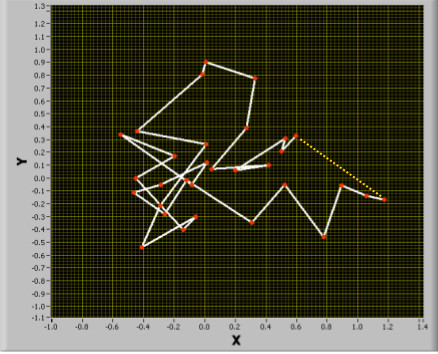
\includegraphics[scale=0.6]{immagine/spezzata.jpg}
\caption{Movimento di una particella nel tempo}
\end{figure}
Abbiamo un programma che simula il movimento di una particella siffatta mediante l'attribuzione di una certa costante di diffusione.
I punti sulla traiettoria spezzata sono le posizioni assunte dalla particella ogni 10 millisecondi. Ogni movimento non tende linearmente ad allontanarsi rispetto al punto di origine e possiamo avere addirittura un ritorno sulla posizione iniziale; le deviazioni sono date dalle collisioni ed esse fanno sì che se noi delimitiamo uno spazio e ci chiediamo la probabilità che la particella esca da questa area è bassissima. Al più dei casi infatti la particella ne rimane all'interno e se vediamo la distanza tra il punto finale ed il punto di partenza, si nota che spesso è molto breve.

Questo processo si chiama \emph{collisione libera} perché non c'è alcuna barriera a facilitarla o ad ostacolarla. Distinguiamo un percorso medio netto, quello tratteggiato in giallo, che unisce inizio e fine. Se noi andassimo a tutti i percorsi singoli invece, avremo una distanza percorsa molto più grande.

Come sono legati spazio e tempo? Data una certa distanza, quant'è il tempo necessario per fare un percorso netto di quella lunghezza? 
Albert Einstein studiò questo fenomeno e produsse questa relazione: il tempo necessario a percorrere lo spazio in 3 dimensioni (ecco perchè 6) è dato da:

\begin{equation}
\centering
t=\frac{s^{2}}{6D}
\end{equation}

dove D è la \emph{costante di diffusione} ($\frac{cm^{2}}{s}$): dipende dalla \emph{dimensione della particella}, dall'ingombro che l'oggetto incontra nel traslare nell'acqua : D in questo caso è equivalente all'ingombro creato da una sfera di pari diametro del nostro oggetto. Questa particella è piccolissima (anione proteico o uno ione potassio) e può avere dimensioni diverse e in più, oltre alla dimensione, noi possiamo avere diverse caratteristiche peculiari. 
Relativamente alla diffusione libera, qual è l'ingombro che questo oggetto incontra a traslare nell'acqua?

Siccome una proteina può ruotare, è come se fosse una sfera. A parità di agitazione termica, un oggetto come lo ione va più lontano rispetto ad uno come una proteina, che ruota.
Quando noi definiamo costante di diffusione ci riferiamo alla \emph{facilità di traslare all'interno del solvente}.
Oggetti più piccoli hanno costante di diffusione maggiore. 

es. Potassio: $2e^{-5}$ ; Proteine: $1e^{-7}$

Stimando invece una membrana di una cellula, la \emph{distanza tra parte interna ed esterna} è di 70 \AA, ovvero 7 nm.
Il \emph{diametro} della cellula è circa 40 $\mu m $, e la distanza massima tra una cellula e un capillare sanguigno è circa $1 mm$.
Proviamo a vedere di calcolare, attraverso il programma e la formula, quanto è il tempo di attraversamento della membrana con la \emph{diffusione libera} e troviamo che è circa $4 ns$.
 È molto basso, quindi attraverso questo meccanismo è molto facile il movimento dato dalla semplice agitazione termica. Se mettiamo 40 nm di distanza invece di 7, servono centinaia di millisecondi! Questo spiega perchè nel citoplasma è difficile creare differenze di potenziale. Se mettiamo 1000 nm, si passa ai minuti!
\begin{figure}[H]
\centering
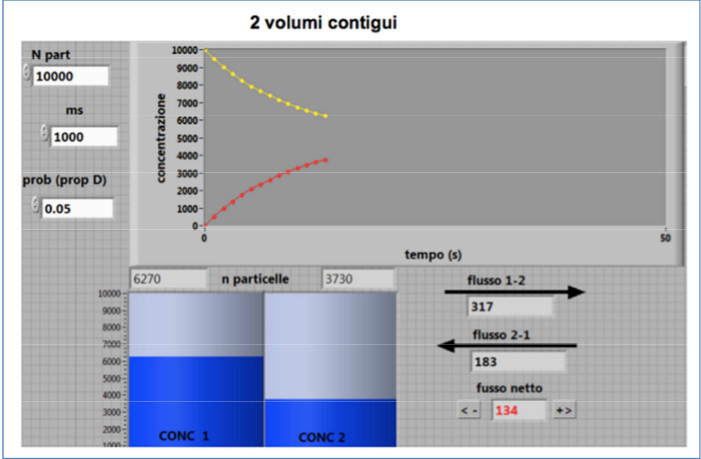
\includegraphics[scale=0.5]{immagine/diff.jpg}
\caption{Coefficiente di diffusione}
\end{figure}

Notiamo dunque che per questo processo è molto efficace il movimento dovuto alla diffusione libera.
Se invece mettiamo una distanza pari al diametro cellulare vediamo che uno ione potassio impiega 133 millisecondi ad attraversarla.
Cosa succede se mettiamo 1000 micrometri? otteniamo 3 minuti per passare da una cellula ad un capillare. Se invece andiamo oltre con 10 millimetri otteniamo 2 ore.
Se invece cambiamo il coefficiente di diffusione (ad esempio per una proteina), abbiamo 26 s. Cosa vuol dire?

Le vaire molecole e ioni differiscono per la loro \emph{motilità} (costante di diffusione). Se una sostanza è molto mobile come il K, basta incrementare lo spazio per avere una relazione \emph{esponenziale}.
Concludiamo che i sistemi di diffusione sono importantissimi perchè, unicamente affidati all'agitazione termica\footnote{quindi praticamente spontanei a certe temperature}, garantiscono la traslocazione di molecole o ioni che, se in spazi limitati, è efficentissima, ma se superiamo certi spazi, spessori, il sistema assume esponenzialmente un ritardo tale da essere incompatibile con la vita. 


L'impulso nervoso viene realizzato in 2 ms. Ogni impulso fa passare delle picomoli di ioni attraverso la membrana: ciò è possibile sfruttando l'energia termica, purchè le distanze siano brevi. Man a mano che esse crescono, questo fenomeno diventa sempre più limitato.

\paragraph{Esperimento}
Beker con dentro acqua, ci mettiamo una massa di sostanza colorata. Supponiamo che la sostanza si composta da molecole non cariche: la sostanza si idrata, si dissocia. Ciò che osserviamo dipende dal tempo:
\begin{itemize}
\item{All'inizio tutto bianco}
\item{Man a mano la colorazione aumenta}
\item{All'equilibrio abbiamo una \emph{situazione stazionaria}: ciò è dovuto alla \emph{diffusione libera}}
\end{itemize}

Questo fenomeno è dovuto alla \emph{diffusione libera}.


Immaginiamo di isolare un sistema con due compartimenti, inizialmente divisi: da una parte solo solvente, dall'altra anche il soluto ad una certa concentrazione. Al tempo 0 togliamo la separazione: le particelle passano dalla zona a concentrazione maggiore a quella a concentrazione minore ed i livelli tendono ad eguagliarsi fino ad arrivare ad una situazione di equilibrio.
Consideriamo che c'è un flusso da entrambe le parti.

Questo processo avviene perchè le molecole di colorante si comportano come la particella della quale parlavamo prima.

Il flusso netto all'equilibrio diventa anche negativo, perchè il numero delle particelle dalle due parti non è proprio ugale, simile ma non uguale. A volte prevale una concentrazione, a volte l'altra. Questo è un tipo di \emph{equilibrio dinamico}.


\paragraph{Perché se mettiamo in un distretto del sistema una quantità di particelle, si assiste al passaggio di particelle dal distretto più concentrato al meno concentrato?}
È una questione di statistica. . Se assegniamo ad una particella la probabilità di passare da un distretto all'altro e viceversa e questa è uguale per ogni particella, è chiaro che il numero di particelle, a parità di probabilità, che passerà da un compartimento in cui sono più numerose a uno in cui sono di meno, sarà maggiore del numero di particelle che passerà dal compartimento a concentrazione minore a quello a concentrazione maggiore. Questo è fondamentale e ci fa capire perché si insista tanto sulla diffusione libera.

\paragraph{}
La diffusione libera è un motore naturale di straordinaria potenza perché apparentemente non costa nulla, costa solo la temperatura. La temperatura di un sistema produce il processo di diffusione libera, la quale diffusione libera, se siamo in condizione di salto di concentrazione, crea proprio un potenziale capace di compiere lavoro. Il lavoro che compiamo in questo caso è il trasferimento delle particelle.

Non c'è un vettore \emph{forza}: le particelle sentono la temperatura, agitano termicamente e diffondono, tendendo statistaticamente ad occupare il massimo dello spazio.

Se siamo in condizioni di una salto di concentrazione, la diffusione libera crea un vero e proprio \emph{potenziale} : energia potenziale capace di compiere lavoro, che è il trasferimento delle particelle in questo caso.
Non ci sono forze che spingono la particella a passare da un lato all'altro! Le particelle sentono la temperatura, si agitano termicamente e diffondono, tendendo ad occupare il massimo dello spazio.
\subsection{Flusso}
Definiamo i concetti di:
\begin{itemize}
\item{Flusso unidirezionale: sposta particelle in un'unica direzione (1 \lfreccia 2 o 2 \lfreccia 1)}
\item{Flusso netto: differenza tra i flussi unidirezionali}
\end{itemize}

Il flusso unidirezionale dipende dalle \emph{concentrazioni assolute}, mentre quello netto dalla \emph{differenza di concentrazione} tra le due parti.

\textbf{Recapitolando} \ldots

Esiste un motore naturale dato dall'\emph{agitazione termica} che crea spostamento di materia in una soluzione e può compiere lavoro. Il lavoro compiuto è più efficace se realizzato su percorsi brevi.

Il trasferimento di ioni avviene in una direzione in dipendenza dalla concentrazione del compartimento di origine.
I flussi sono due, uno decresce e uno cresce, fino ad equalizzarsi a livello statistico. Il flusso 1-2 direzionale dipende direttamente dalla concentrazione di 1.

Abbiamo considerato due regioni contigue di una soluzione in cui una delle regioni presenta una concentrazione maggiore di soluto che per ora consideriamo generico (cioè carico o non carico). Facciamo un esempio semplice di un soluto non carico:
\begin{figure}[H]
\centering
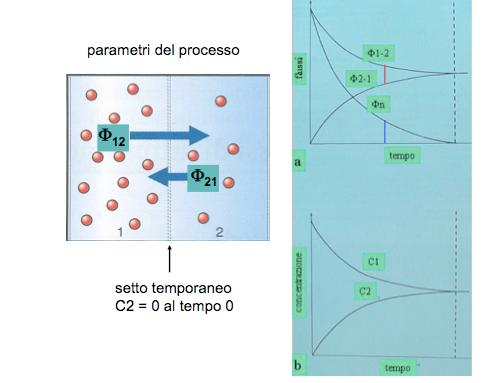
\includegraphics[scale=0.5]{immagine/potenziale.jpg}
\caption{}
\end{figure}

Abbiamo visto qual è la condizione della diffusione sotto forma di due flussi identificabili: 
\begin{enumerate}
\item{Flusso unidirezionale dal primo al secondo compartimento}
\item{Flusso unidirezionale dal secondo al primo compartimento}
\end{enumerate}

e poi un \emph{flusso netto}, ciò non fa che riassumere quello che si è già detto identificando i flussi con questi vettori in cui il modulo è proporzionale all' intensità del flusso.

La cosa da ricordare è che la dipendenza del flusso 1-2 unidirezionale è direttamente proporzionale alla concentrazione $C_{1}$ del compartimento di partenza, così come il flusso 2-1 dipende dalla concentrazione $C_{2}$ soltanto.
Quindi i flussi unidirezionali dipendono unicamente dalla concentrazione di origine mentre il flusso netto,  inizialmente molto alto, tende ad azzerarsi in media quando lo fanno anche i due flussi unidirezionali. Quindi la differenza fra $C_{1}$ e $C_{2}$ si riduce.

\begin{figure}[H]
\centering
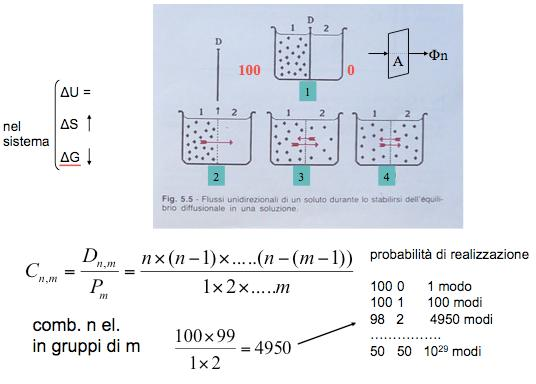
\includegraphics[scale=0.4]{immagine/combinatorio.jpg}
\caption{}
\label{img:comb}
\end{figure}


\paragraph{$\Delta U$: Energia interna}
Per capire bene i fenomeni alla base della fisiologia animale consideriamo un sistema termodinamico in cui l'energia interna\footnote{legata cioè all'agitazione termica e al potenziale chimico} nell' intero sistema non cambia, perché abbiamo un energia interna che passa da 1 a 2, ma l'intero sistema non la vede cambiare.

\paragraph{$\Delta S$: Entropia}
è un concetto ampio usato in molti modi diversi. Termodinamicamente parlando è una variabile definita sempre come differenziale, che è associata allo stato di ordine o disordine del sistema.
In un sistema lasciato a sé, l'entropia tende ad aumentare (si è già visto nell'esempio del topo con il formaggio).
Durante il differenziamento cellulare del topo, alcuni blastomeri non sono identici ad altri ma differenti e col passare del tempo questa differenza andrà a sfociare nella formazione di \emph{tessuti diversi}. Così facendo si crea un disordine del sistema: ma questo significa che durante lo sviluppo un sistema vivente lavora contro la tendenza entropica, che tenderebbe a rimescolare tutto.
Se un sistema viene lasciato a sé, spontaneamente viene portato al disordine.
Non fa eccezione il sistema in figura \ref{img:comb} cui possiamo vedere l'ordine tutto a sinistra (oppure ognuno dove vuole) e a destra il disordine. Se il sistema è in moto abbiamo che l'entropia aumenta.

\paragraph{$\Delta G$: energia libera di Gibbs}
Un sistema termodinamico può variare poiché l'energia interna, entalpia ed entropia e consumo netto di queste variazioni si ripercuote in un cambio di energia libera:
\begin{equation*}
\centering
dU=-TdS 
\end{equation*}

Significa che, definite queste variazioni, so come cambia l'energia libera.

L' energia libera è la \emph{capacità di compiere lavoro}.
Un sistema può compiere lavoro se ha un'energia libera a cui attingere. Se invece degrada al minimo valore l'energia libera, non può più compiere lavoro.

\paragraph{Esempio} il sistema in figura \ref{img:comb} allo stadio in cui vediamo il setto divisorio fra 1 e 2 è un sistema capace di compiere lavoro. la cellula utilizza queste differenze di concentrazione per spostare i soluti o nella stessa direzione della riduzione di concentrazione o in senso opposto, il che significa che capire bene come funzionano questi meccanismi è importante per capire come la cellula sfrutti questo motore cellulare, che per brevi percorsi è di importanza vitale.

L'energia libera da un massimo passa poi ad un intermedio ed arriva ad un minimo. Il lavoro che l'energia libera compie è quello di spostare soluti.
La forza che spinge le particelle non è un vettore, come sarebbe se le particelle fossero cariche e noi mettessimo un campo elettrico come nell'elettrolisi (in quel caso il vettore campo elettrico si applica ad un a particella carica), ma è un \emph{fenomeno statistico}.
Se da una parte abbiamo più particelle e dall’altra meno e le particelle hanno la stessa probabilità di diffondere in un certo tratto, ho più probabilità che il maggior numero di particelle si spostino verso la concentrazione minore di particelle.

\subsection{Potenziale chimico}
Consideriamo il sistema come se fosse termodinamico:
l'energia interna, legata all'agitazione termica e al potenziale chimico, non cambia nell'intero sistema, perchè si "travasa " da 1 a 2; cambia però la componente entropica.

Ci possiamo chiedere perché la situazione 2 in figura \ref{img:comb} è instabile e la 4 è fortemente stazionaria, e lo possiamo risolvere in termini statistici.

Supponiamo di avere 100 particelle e 2 posizioni: se impostiamo il problema in termini combinatori, dobbiamo calcolare la combinazione di N elementi in gruppi di N:
\begin{equation*}
\centering
C_{n,m}=\frac{D_{n,m}}{P_{m}}=\frac{n * (n-1) \ldots *(n-(m-1) }{1*2 \ldots *m}
\end{equation*}

Se abbiamo 100 particelle da una parte e 0 dall'altra abbiamo un solo modo di realizzare questa configurazione, mentre abbiamo 100 modi se vogliamo metterne 99 particelle da una parte e 1 dall'altra perché una può essere permutata da tutte e 100 e così via.
Se invece abbiamo 50 particelle da una parte e 50 da un'altra, ottengo $10^{29}$ combinazioni possibili.

Quindi un sistema stazionario è un sistema che ha alta probabilità di permutazione, mentre più è ordinato più si discosta da questa. Da ciò deriva che se voglio spostare un sistema che spontaneamente andrebbe verso una parte, dalla parte opposta reversibilmente, devo applicare energia, devo lavorare contro questa tendenza spontanea.
Tutti i sistemi tendono spontaneamente ad aumentare l'entropia e a ridurre l'energia libera.

Vediamo formalmente come si definisce questa capacità di compiere lavoro legata alla concentrazione e dipendente dal processo di diffusione libera.
\begin{figure}[H]
\centering
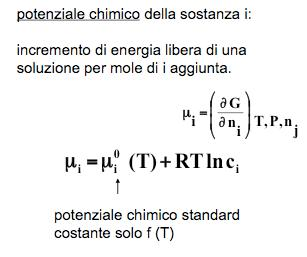
\includegraphics[scale=0.4]{immagine/pot_chimico.jpg}
\caption{}
\end{figure}

Chiamiamo \emph{potenziale chimico} l'espressione nella slide $\mu_{i}$ :
\begin{equation}
\centering
\mu_{i}=(\frac{\delta G}{\delta n_{i}}) T, P, n_{j}
\end{equation}

(dove i è la sostanza i-esima contenuta in una soluzione con altre specie). 

Chiamiamo $\mu_{i}$ l’incremento di energia libera di una soluzione per mole di $i$ aggiunta mantenendo le altre J-esime specie chimiche uguali e tenendo T e P costanti.
Se calcolo il cambio di energia libera in funzione di una mole aggiunta ho $\mu$ di una specie i esima.

Non abbiamo quindi un $\mu_{i}$ assoluto ma relativo.
Tutte le specie hanno un potenziale standard proprio.
Saputa la sostanza $\mu_{i}$ si mette in funzione della temperatura:
\begin{equation}
\centering
\mu_{i}=\mu_{1}^{0} RT ln c_{i}
\end{equation}

Quindi il potenziale chimico dipende da una costante per la relazione logaritmica con la concentrazione della sostanza.
Il flusso lo possiamo indicare con $\Phi$, siccome abbiamo scelto un certo divisorio con una certa area, il flusso dipenderà da questa.
\begin{figure}[H]
\centering
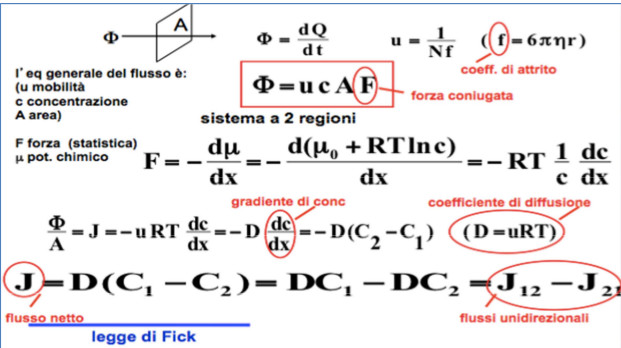
\includegraphics[scale=0.5]{immagine/conti.jpg}
\caption{Come ricavare la legge di Fick}
\end{figure}
Allora chiamiamo flusso la quantità spostata nell'unita di tempo e quindi: 
\begin{equation}
\centering
\Phi=\frac{dQ}{dT}
\end{equation}

Guardiamo la relazione di $\Phi$ (in altro al centro inquadrata di rosso) la legge che regola la dipendenza fra flusso e la forza statistica che muove le particelle: è una legge generale che io potrei scrivere: $i = fC$.
  
Facendo un esempio: ricordando la legge Ohm $V=i R$ (V= differenza di potenziale , i = corrente , R= resistenza), la resistenza fa si che il cambio di voltaggio produca una corrente inversamente proporzionale. È come dire che se abbiamo una batteria con due poli, fino a che questi sono aperti noi non abbiamo corrente; se poi costringiamo i due poli con un conduttore, questa legge ci dice che la corrente che fluisce è inversamente proporzionale alla resistenza del conduttore.

Ciò significa che \emph{l'impedimento al passaggio delle cariche che il conduttore offre condiziona il flusso}.
\begin{equation}
\centering
I=G \Delta V
\end{equation}
è la legge di Ohm scritta in termini generalizzati.

La ritroveremo in molti altri casi di flussi in questa forma :
\begin{equation}
\centering
F=\frac{1}{R} PV 
\end{equation}

Abbiamo una equazione equivalente che descrive il flusso di un fluido, tralasciando la resistenza del condotto, in dipendenza dalla differenza di pressione ai due capi del condensatore (PV).
Allora la differenza di pressione ai due capi è un’\emph{energia potenziale}.

Il flusso è un flusso di carica e di acqua, questo permette di generalizzare e dire che c'è un \emph{equazione generale di Teorell}: un qualsiasi flusso lo posso generalizzare dicendo che dipende dalla F coniugata a meno della resistenza.
\begin{equation}
\centering
\Phi= u c A F
\end{equation}

Con $u$ (mobilità) si vuole descrivere il fatto che ogni cosa che si muove sotto questi gradienti avrà una facilità o difficoltà a muoversi.

Con questa equazione centrale diciamo che il flusso è dato dalla concentrazione e da distinzioni della superficie di scambio in funzione della mobilità della sostanza.
\begin{figure}[H]
\centering
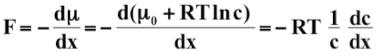
\includegraphics[scale=0.55]{immagine/F.jpg}
\caption{}
\end{figure}

Se esplicitiamo F (forza coniugata), vediamo che in questo caso è data dal salto di concentrazione.
La concentrazione ha come indicatore il potenziale chimico $\Delta \mu$ ecco che noi diciamo che f sarà il potenziale chimico in funzione dello spazio $\Delta X$ , perché il nostro compartimento vede cambiare la concentrazione nello spazio.
Notiamo un segno – : esso viene perché la forza premente che spinge va in direzione opposta a come aumenta in gradiente di concentrazione.
\begin{figure}[H]
\centering
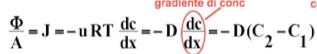
\includegraphics[scale=0.6]{immagine/fi.jpg}
\caption{}
\end{figure}

dove D è il coefficiente di diffusione ed è uguale a $uRT$.

Quindi ottengo in somma sintesi che J, il flusso netto, è uguale:
\begin{equation}
\centering
J=\frac{- \Delta C}{\Delta X} 
\end{equation} 
che è il \emph{gradiente di concentrazione}.

Esplicitando, J è esprimibile così: 
\begin{equation}
\centering
J=D (C_{2}-C_{1})
\end{equation}

Questa è la \textbf{legge di Fick}.

L'ultima parte dell'ultima equazione non sono altro che i flussi unidirezionali che dipendono unicamente dalla concentrazione del compartimento di origine.

\emph{Per quale motivo viene anche descritta in funzione della distanza?}

In realtà, il gradiente di concentrazione, espresso come differenza, può essere visto in due modi: se abbiamo un certo ambiente acquoso e da una parte una grande concentrazione e dall'altra una minore, il potenziale elettrochimico sarà in funzione della distanza tra i due punti. Il gradiente di concentrazione ha quindi un valore diverso nei due punti. Prendiamo due volumi isopotenziali (uniformemente distribuiti) e stabiliamo attraverso un'area A quanto scambiano. La legge si considera quindi per area di scambio unitaria e per distanza unitaria.

\section{Elettrodiffusione, compartimenti e barriere}
Fin'ora abbiamo trattato di soluti non carichi (come il saccarosio); se consideriamo uno \emph{ione}, esso è anche suscettibile ad un \emph{campo elettrico}, poichè possiede una carica. Se abbiamo una ddp tra due punti e degli ioni interposti, gli anioni verranno attratti dal polo positivo ed i cationi dal polo negativo.

Se mettiamo in soluzione e consideriamo i compartimenti come fatto finora, ma non più per un soluto non carico, dobbiamo aggiungere alla descrizione della legge di Fick una parte che ha attinenza col \emph{comportamento elettrico}.

Così come abbiamo descritto un \emph{potenziale chimico} per le sostanze cariche e non cariche, per quelle cariche dobbiamo introdurre un \emph{potenziale elettrochimico}:
\begin{equation}
\centering
\mu= \mu_{i}^{0}(T) + RTlnc + z_{i}F\psi
\end{equation}\todo{metti mu soprasegnato}
				
dove $z_{i}F\psi$ è il \emph{potenziale elettrico}. Dato che si tratta di ioni dobbiamo considerare che i coulomb trasportati da ogni mole di ione monovalente è uguale alla costante di faraday per la valenza ($z_{i}$ è la valenza dello ione, $\psi$ è l'energia potenziale elettrica espressa in J/C e F la costante di Faraday).
Rispetto al potenziale chimico, per calcolare il potenziale elettrochimico ($\mu$ barrato) di uno ione aggiungiamo questo fattore $z_{i}F\psi$.

Se nei due compartimenti considerati nella scorsa lezione anziché del saccarosio mettiamo uno ione, se è presente un campo elettrico tra le regioni 1 e 2, la legge di Fick diventa:
\begin{equation}
\centering
J_{A} = D(C_{1}-C_{2}) + z_{i}k(V_{1}-V_{2}) 		
\end{equation}

dove c'è un elemento permissivo che è la conduttività della soluzione ($z_{i}k$). Il flusso netto fra i due compartimenti sarà pari ad un addendo relativo alla legge di Fick e un altro che è la legge di Ohm.

Questa è l'\emph{equazione di elettrodiffusione di Nernst-Plank} e ci permette di calcolare un flusso tra due compartimenti che differiscono per:
\begin{enumerate}
\item{Concentrazione della specie che consideriamo}
\item{Differenza di potenziale elettrico tra le due zone}
\end{enumerate}

\paragraph{Caso 1}
Se mettiamo due molecole non cariche in due compartimenti a concentrazione diversa, c'è già un potenziale che compete allo spostamento di queste particelle da un'area a maggior concentrazione ad una a minor concentrazione,  e quindi
si considera nell’equazione J solo il primo temine (Fick).

\paragraph{Caso 2}
Se questa specie è carica possono succedere tre cose:
\begin{enumerate}
\item{Fra i due compartimenti non ci sono differenze di potenziale chimico pur essendo la specie carica (legge di Fick)}
\item{Fra i due compartimenti non ci sono differenze di potenziale chimico, ma c’è una differenza di potenziale elettrico. Le cariche sono distribuite ugualmente nei due compartimenti.
Esempio: nel compartimento 1 ho 3 particelle con valenza 2+ ciascuna, nel 2 ho sempre 3
particelle ma con valenza 1+.
Quindi in questo caso nell’equazione J considero solo il secondo termine (Ohm)}
\item{Se abbiamo tutte e due: equazione di elettrodiffusione di Nernst-Planck}
\end{enumerate}

Se conosciamo nei due compartimenti le concentrazioni di una specie, la carica e la differenza di  potenziale elettrico tra i due compartimenti, possiamo calcolare il flusso conoscendo la costante di diffusione libera, la valenza e la costante k che dà la conduttività.

\subsection{Come si introduce in un contesto biologico?}

Nella cellula animale:

\begin{itemize}
\item{Ambiente interno : soluzione nella quale sono immerse le cellule , il \emph{liquido interstiziale o extracellulare}}
\item{Compartimento intracellulare}
\end{itemize} 

\paragraph{Compartimento} è uno spazio delimitato da \emph{barriere}, le quali sono strutture capaci di interferire con il passagio di soluti tra compartimenti. Es endotelio capillare (separa liquido plasmatico da liquido extracellulare), la membrana cellulare. La barriera è capace di interferire col libero passaggio delle sostanze tra compartimenti diversi in modo selettivo o non selettivo.
\paragraph{}
Assumiamo che tutte le barriere siano permeabili all'acqua, in modo maggiore o minore. Ci sono 2 diversi meccanismi che permettono alle molecole d'acqua di passare da un compartimento all'altro: 
\begin{enumerate}
\item{Dato dalla temporanea inconsistenza del doppio strato lipidico, quindi una membrana che è tra le più selettive barriere che consciamo, può permettere a causa dell'agitazione termica che tende a scollare molecole del doppio strato lipidico \lfreccia qualche  molecola d'acqua può passare}
\item{Far passare acqua attraverso delle strutture persistenti, i \emph{canali ionici}, porosità molecolari della membrana riempite costantemente di acqua. Per quanto sia una permeabilità misurabile, ha un'efficienza piuttosto bassa. Le barriere che vedremo in organi che regolano la permeabilitò dell'acqua, come il rene, in aggiunta a questo varco inseriscono le \emph{acquaporine}, ad alta efficienza per il passaggio di acqua}
\end{enumerate}
 
L'interferenza della barriera al passaggio dei soluti può presentare diversi gradi di selettività:
\begin{itemize}
\item{Membrana plasmatica: selettività altissima. Fa passare bene il K, non così il Na. Sono entrambe monovalenti, per questo selettività altissima}
\item{Una barriera può distinguere cationi da anioni, i bivalenti rispetto ai monovalenti, ioni di tipo salino da ioni proteici (selettività inferiore)}
\end{itemize}

Quanti compartimenti abbiamo in una cellula relativamente all'ambiente interno? 

Diversi e di diversa natura. L'interferenza della barriera al passaggio dei soluti può essere più selettiva o meno selettiva.
Quello che vediamo è quindi:
\begin{itemize}
\item{Spazio delimitato dalla membrana}
\item{Spazio intracellulare, che contiene vari sistemi membranosi: membrana nucleare, RE, AG, mitocondri\footnote{selettività per ioni bivalenti} ecc. Ognuno di questi organelli è delimitato da una membrana, quindi ciascun liquido luminale\footnote{relativo al lume dell'organello} è separato dal citosol tramite una membrana. Ogni volta che identifichiamo un organello delimitato da membrana, distinguiamo un \emph{compartimento luminale} e un \emph{compartimento citosolico}}
\end{itemize}

La caratteristica generale di un compartimento è quella di presentare, mediamente (in un lungo tempo di osservazione), una \emph{composizione costante}, a meno di variazioni della permeabilità delle barriere o della concentrazione di uno dei due compartimenti. Questo perchè, ad esempio nel liquido extracellulare, se si creasse una variazione di concentrazione locale, immediatamente la diffusione libera  annullerebbe questo potenziale chimico.

Tra i compartimenti intracellulare ed extracellulare osserviamo invece \emph{differenze di composizione} dovute alla diversa \emph{selettività delle barriere}.

In una stessa regione consideriamo la concentrazione costante, perciò si parla di \emph{comportamento isopotenziale}.

Per capire questo facciamo un passo indietro: cos'è una differenza di potenziale elettrico? È una situazione in cui due cariche sono separate, ovviamente serve lavoro. Supponiamo quindi che si crei una differenza di potenziale tra due punti del compartimento : può essere annullata dallo \emph{spostamento di cariche} o dalla variazione di concentrazione, poichè siamo nello stesso compartimento e non ci sono barriere.

Il flusso ripristina l'omogeneità, così se c'è un cambio di potenziale elettrico, immediatamente viene annullato con spostamento di cariche (ioni). Immaginiamo che la differenza di potenziale si crei all'interno di uno stesso compartimento perchè ioni negativi si accumulano in un certo punto: questo è statisticamente molto improbabile perchè ciò creerebbe una ddp e una differenza di concentrazione \lfreccia l'equazione di nerst e planck si annullerebbe. \emph{Isopotenzialità} significa che se mettiamo in due punti qualsiasi dello stesso compartimento due elettrodi, che tentino di misurare la ddp troviamo ddp = 0.


\subsubsection{Barriere}
Ogni cellula si colloca ad una distanza < 1mm da un capillare\footnote{Parte del sistema circolatorio deputata agli scambi con i tessuti}, perchè la diffusione libera, il \emph{motore degli scambi}, ha efficienza fino a queste distanze.


\paragraph{Endotelio capillare}
La prima barriera che delimita il capillare, caratterizzata da cellule endoteliali giustapposte, ma non saldate. Tra esse si creano degli spazi intercellulari, che nel nostro organismo sono più o meno ampi.
\begin{figure}[H]
\centering
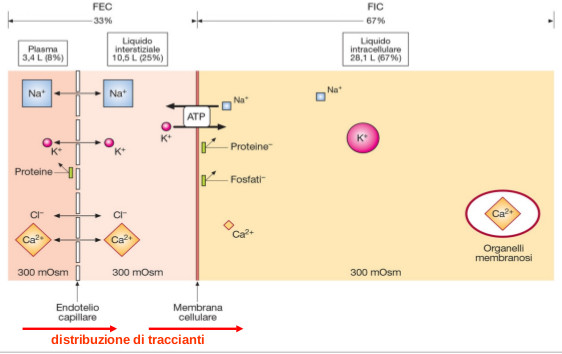
\includegraphics[scale=0.45]{immagine/endotelio.jpg}
\caption{Schema rappresentativo delle barriere endotelio capillare e membrana cellulare}
\label{img:endo}
\end{figure}

Possono essere molto stretti come ad esempio nel nostro encefalo (parla di barriera ematoencefalica, riduzione di permissività di passaggio di molecole che ha lo scopo di proteggere la stanza dei bottoni dell'encefalo dall'inquinamento con molecole estranee), oppure possono essere dei pori che sono più o meno ampi e li troviamo in varie regioni; in tutte però esiste una condizione per cui, attraverso questi pori, possoo passare non solo acqua ma anche tutti i soluti sia carichi che non.
Si parla in questi casi di \emph{flusso di massa}, vale a dire che fra queste due regioni può passare non glucosio attraverso una via e sodio attraverso un’altra ma tutta la soluzione con tutti i sui soluti e solventi. La ricaduta di questa condizione la vediamo analizzando la \emph{composizione} dei due compartimenti.

Il liquido intracellulare è circa il 67\% del liquido totale e questi due compartimenti sono l'8\% e il 25\%: questa distribuzione dei liquidi (plasma, liquido interstziale e liquido intracellulare) si valuta grazie a traccianti che passano una barriera, ma non l'altra. Ogni componente nella figura \ref{img:endo} ha un simbolo, più grande o più piccolo, che si riferisce alla concentrazione, maggiore o minore. Il Na ha due quadrati della stessa entità: se ne titoliamo la quantità nel plasma, la troviamo identica a quela nel liquido extracellulare. Nei liquidi intracellulari\footnote{delimitati dalla membrana plasmatica} invece c'è una caduta brusca della concentrazione di Na: è una \emph{situazione stazionaria}, la cellula non è stimolata \lfreccia la barriera tra liquido interstiziale e intracellulare non è selettiva per il Na, per il K, per il Cl e per il Ca. 

Le uniche specie interdette sono le \emph{proteine}, presenti nel plasma sanguigno ma pressoché assenti nel liquido extracellulare.

\paragraph{Membrana palsmatica}

Il calcio libero nel citosol ha una caduta di concentrazione enorme (non tutto, infatti se titoliamo troviamo grandissime quantità di calcio che poi sono sequestrate da RE e mitocondri). Se facessimo una titolazione di \emph{tutto il Ca}, troveremmo una quantità enorme, che viene catturata all'interno di organelli come il RE ed i mitocondri. 

Di Cl all'interno ce n'è poco, ma vi troviamo anioni proteici e anioni fosfato.

Se misuriamo la \emph{osmolarità}\footnote{L'osmolarità è la pressione osmotica generata dai soluti presenti in 1 L di solvente} di un compartimento, definiamo sia la composizione in concentrazione di ogni componente, sia la valenza osmotica (sommando tutti i componenti).

La proprietà di una soluzione di \emph{generare pressione osmotica} è legata alla osmolarità, non alla concentrazione.

Prendiamo una soluzione di NaCl 1 M: quanto sarà l'osmolarità?
Dato che questo sale in soluzione è completamente dissociato avrò osmolarità 2 osmoli. Se andiamo a misurare l'osmolarità ad esempio della soluzione fisiologica che è NaCl 150 M, significa che vale 300 mosm.

Tutti i soluti salini in questione vaglono 300 mOsm (perchè si trovano in soluzione fisiologica, che è 150 mmoli), per le proteine si valuta invece la \emph{pressione oncotica}\footnote{dovuta sia alle proteine che agli ioni salini}.

All'interno delle cellule c'è la stessa osmolarità: l'acqua infatti passa liberamente e se ci fosse un salto osmolare, avremmo o una perdita continua di acqua o un'acquisizione continua di acqua, visto che la membrana è permeabile alla grande. \emph{Nei tre compartimenti analizzati abbiamo quindi composizioni diverse, ma circa la stessa valenza osmotica}. Si può quindi dire che i soluti sono in forte squilibrio qualitativo ma l'acqua ha una distribuzione uniforme dal momento in cui si muove unicamente per \emph{sollecitazione osmotica} che non è altro che un particolare caso di diffusione libera.

Anche la presenza del $K^{+}$ nella cellula ha tantissima valenza funzionale, così come il salto di K e Na nella direzione opposta: ciò permette i fenomeni di \emph{eccitabilità} ed altri feomeni importanti.

\subsubsection{Distribuzione degli ioni}

La concentrazione dei vari ioni nel liquido extracellulare e intracellulare è diversa, così come lo sono le concentrazioni nelle varie cellule: questo dipende infatti dalla selettività della propria membrana. La membrana è infatti una \emph{barriera a selettività specifica} per ogni tipo cellulare e condiziona la quantità di soluti all'interno.

Fissiamo a 140 mmoli la concentrazione del liquido extracellulare. Per il K abbiamo 4/5 mmoli/L di K nel liquido extracellulare e all'interno 120 mmoli/L. Per il Na all'interno abbiamo 14 mmoli/L e 140 all'esterno.
Quindi, o la membrana è impermeabile al K o permette poco passaggio della specie ionica: nel lungo tempo però dovrebbe avere il tempo di uniformare le due concentrazioni all'interno e all'esterno.

In realtà, anche se la membrana è selettiva, deve esserci un altro fattore che tende ad accumulare certe specie e a favorire l'uscita di altre: è il fenomeno dell'\emph{equilibrio di Gibbs-Donnan}. La distribuzione diversa di ioni ubbidisce quindi a 2 proprietà:
\begin{itemize}
\item{Diversa permeabilità della membrana alle diverse specie : altamente permeabile al K, meno al Na}
\item{Equilibrio di Gibbs Donnan}
\end{itemize}

\subsubsection{Permeabilità}
All'esterno domina NaCl, all'interno fosfati e proteinati di K.

\paragraph{$Ca^{2+}$}
Il calcio compie un salto grandissio tra l'esterno e l'interno della cellula: nel plasma circa 2,5 mmoli/L, nella cellula circa 100 nmoli/L.

Nel citosol ce n'è così poco perchè dei meccanismi attivi tendono a trattenere il $Ca^{2+}$ nel RE e nel mitocondrio, lasciandone pochissimo nel citosol; se cio non avviene, si ha un innalzamento dei livelli di $Ca^{2+}$ nel citosol che, se prolungato, è tossico per la cellula. Alcune proteasi vengono infatti attivate dal $Ca^{2+}$ ed iniziano a tagliare enzimi, proteine di membrana \lfreccia attivazione di una cascata di eventi, \emph{apoptosi}, che tende a distruggere il DNA\footnote{il significato biologico è di non disperdere nell'ambiente molecole che danno informazioni}, con conseguente morte cellulare.

Un altro meccanismo per tenere basso il Ca nel citoplasma è di \emph{farlo uscire} dal citoplasma verso il liquido extracellulare.

\paragraph{pH}

Acidificazione del citosol rispetto all'ambiente extracellulare. Questa acidità è dovuta al metabolismo intermedio, che tende a \emph{produrre acido}. Il valore è 7.1-7.2 (rispetto a 7.4 extracellulare).

Queste diverse composizioni non possono derivare solo dalla diversa permeabilità della membrana ai diversi ioni: ciò non garantirebbe infatti la \emph{disomogeneità}, garantita più che altro dall'\emph{equilibrio di Gibbs-Donnan} e, in seconda battuta, dalla permeabilità diversa. Per mantenere la diversa composizione di ioni, dobbiamo quindi \emph{spendere lavoro}\footnote{altimenti alla lunga i sistemi si equilibrerebbero}: nello spessore della membrana esiste un'\emph{ATPasi}, o pompa ionica, che porta il $Na^{+}$ verso l'esterno e il $K^{+}$ verso l'interno, opponendosi al flusso diffusivo, a costo di spesa di ATP.

\subsubsection{Equilibrio di  Gibbs-Donnan}
Visto che nella cellula le proteine predominano come \emph{anioni proteici}, se avessimo solo ioni diffusibili ($Na^{+}$, $K^{+}$, $Ca^{2+}$), al di là dei processi attivi nessun altro fenomeno potrebbe segregare concentrazioni diverse. Se invece abbiamo \emph{anioni intracellulari} che non possono passare attraverso la membrana (anioni proteici e fosfati), essi tenderanno a trattenere cationi diffusibili e permeabili : la membrana è quindi invogliata a trattenere il $K^{+}$, poichè è memo permeabile an $Na^{+}$, che resta all'esterno e trattiene il $Cl^{-}$.

Ecco perchè all'esterno della cellula c'è molto NaCl e all'interno c'è molto K e proteato di K.

Per mantenere la distribuzione dei soluti descritta, la cellula deve compiere lavoro. È fondamentale l'azione delle pompe. Questo si può provare \emph{avvelenando metabolicamente la cellula}: il cianuro interferisce con la fosforilazione ossidativa e la produzione di ATP, oppure veleni come la ouabaina, che interferiscono con l'attività di ATPasi \lfreccia  distribuzione di ioni sempre più omogenizzata.

La disomogeneità del sistema, in termini di entropia, viene mantenuta bassa con spesa di energia (è una situazione di maggiore ordine rispetto a quella in cui le concentrazioni sono più omogenee).


\subsection{Organizzazione di una tipica barriera: la membrana plasmatica}
Vediamo l'organizzazione a livello \emph{sopramolecolare}, poi descriveremo le molecole funzionali che la caratterizzano. È a questo livello che distinguiamo i vari corredi di molecole funzionali dei vari tipi di cellule. Vedremo come funzionano e poi faremo un riepilogo del \emph{traffico delle proteine}: questa struttura non è infatti statica, ma frutto di processi dinamici.

Se vediamo il neurone con degli anticorpi verso certe proteine, possiamo determinare le varie parti del neurone (dendriti, soma, colletto assonico, assone).

\subsubsection{Organizzazione sopramolecolare}
\begin{figure}[H]
\centering
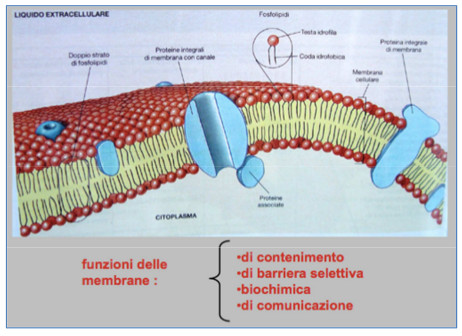
\includegraphics[scale=0.4]{immagine/sopramolecolare.jpg}
\caption{Organizzazione della membrana plasmatica}
\end{figure}

La membrana è composta da un \emph{supporto oleoso} che sono i doppi strati lipidici : è la conformazione termodinamicamente più stabile, per la disposizione dei lipidi. Non ci sono legami tra i fosfolipidi: la posizione è dovuta solo alla repulsione delle code nei confronti dell'acqua.

Immerse parzialmente o totalmente nella membrana vediamo delle \emph{zolle glicoproteiche}, che possono determinare un poro al centro oppure no:
\begin{itemize}
\item{Proteine integrali di membrana: gli aa dell'involucro esterno devono essere \emph{liposolubili}, mentre quelli che guardano l'interno devono essere idrofilici. Possono avere un poro o meno}
\item{Proteine associate: associate alle integrali. Devono avere \emph{adesività}, ovvero dei gruppi che riconoscono le integrali. La tendenza all'associazione è un primo meccanismo di \emph{targeting}.}
\end{itemize}

Anche se associata ad una certa funzione, nella realtà della membrana quella proteina non potrebbe funzionare come tale se non avesse una serie di proteine associate, che ne modulano il livello di attività. I \emph{complessi proteici} sono l'unità funzionali.

Tutte queste proteine devono ovviamente avere \emph{relazioni con il citoscheletro}, legami reversibili non covalenti, che superano la sollecitazione dell'energia termica, ma si formano e disfano più e più volte: proteine di un certo tipo sono nello stesso posto perchè il numero di legami con il citoscheletro in quella regione è statisticamente più alto.

\paragraph{Funzioni della membrana}
\begin{enumerate}
\item{Funzione meccanica, di contenimento: la membrana è una struttura tenuta da minimi energetici, non da legami. Tutte le altre conformazioni di questo sistema sarebbero legate ad un'energia più alta (e quindi meno stabili). Per rompere questo legame, basta azionare una forza meccanica: quella del citosol però non è abbastanza e la membrana diventa un dispositivo di contenimento.  Entro una certa misura la membrana riesce anche a contenere delle reazioni osmotiche: se la cellula è messa in ambiente ipotonico tende ad assumere acqua e quindi a rigonfiarsi. Se il fenomeno però è troppo grande, si ha lisi : al microscopio a contrasto di fase vediamo una bolla, un sacchetto di gel che fuoriesce}
\item{Funzione di barriera selettiva : avendo molecole particolari, la densità nell'unità di superficie dei canali per le varie specie condiziona la permeabilità della membrana alle varie specie}
\item{Funzione biochimica : nella fosforilazione ossidativa\footnote{rivedi in biochimica}, le molecole sono una accanto all'altra in cascata, quindi la probabilità di incontrare un reagente è più alta\footnote{come per i complessi enzimatici}. Una reazione è efficace o meno se avviene in ambito spaziale ristretto o meno}
\item{Funzione di comunicazione: cellule diverse devono poter comunicare. Cellule utilizzatrici devono comunicare il grado di utilizzo di certe risorse, quelle produttrici devono comunicare il grado di produzione. Le due modalità di comunicazione sono quella \emph{nervosa} o \emph{endocrina} (chimica): sono equivalenti a livello evolutivo, ed hanno in comune l'interazione di molecole con membrane (es recettori). Ecco che il \emph{dove disporre} e il \emph{cosa disporre} sulla membrana, la rende \emph{competente a leggere un centro tipo di messaggio}: la noradrenalina è una sostanza prodotta fin quando l'organismo è sollecitato da stimoli associati all'aggressione e alla fuga\footnote{come quando fai l'esame! Il pericolo del professore è invece che si abbassa la noradrenalina (non ci sono ancora casi in cui il professore si sia addormentato)}. Essa va in determinate cellule cardiache e respiratorie e viene letta da quelle cellule, non dall'epatocita ecc. Se quella cellula ha un recettore specifico per quella sostanza risponde; se ne ha molti risponde molto e viceversa}
\end{enumerate}

L'effetto di sostanze endogene (farmaci o droghe) è sempre minore ,via via che si assumono più volte, a parità di concentrazione. Questo è legato al fatto che le cellule lentamente riducono, se è presente frequentemente la sostanza, il numero di recettori.
Nel caso del nervoso i motoneuroni producono neurotrasmettitore, l'acetilcolina, che letta dal versante cellulare da recettori acetilcolinici.
Dobbiamo quindi considerare la membrana come un \emph{fulcro} nella funzione di comunicazione.

Di recente si è inoltre scoperto che il doppio strato lipidico non è un supporto alle poteine, ma anche la parte lipidica ha una sua biochimica: esistono enzimi nella membrana, le \emph{fosfolipasi}, che possono andare su certe componenti dello strato lipidico e dissociarle \lfreccia le molecole prodotte inducono risposte all'interno della cellula.

\subsubsection{Come si muovono le molecole all'interno della membrana?}
L'organizzazione molecolare descrive i componenti: i fosfolipidi, le proteine accessorie etc..
l'organizzazione sopra molecolare invece riguarda l'organizzazione ad un livello superiore.
In genere comunque le interazioni tra queste molecole le troviamo stazionariamente operanti anche se spesso sono legate ad interazioni deboli, nonché vicine e quindi abbiamo una stabilizzazione statistica, fatta di attacchi e di distacchi.

Le \textbf{molecole lipidiche} possono liberamente ruotare, diffondere lateralmente mantenendosi ordinatamente disposte o traslare. Il flip flop è invece è raro se non improbabile: la testa, pur essendo idrofila, dovrebbe attraversare la regione idrofoba. 

Questi cambiamenti di posizione sono tuttavia responsabili della possibilità del passaggio di una molecola d'acqua e testimoniano la tendenza del doppio strato a staccarsi, se sollecitato ulteriormente.


Le \textbf{proteine} non possono muoversi proprio liberamente. Esse possono muoversi \emph{lateralmente}, la torsione invece è vincolata moltissimo perchè tutte le interazioni conferiscono alle proteine pochi gradi di libertà. Il flip-flop per loro non esiste.

L'entità del movimento invece dipende dalla proteina e dipende dalla cellula: ciascuna molecola proteica differisce per essere integrale, accessoria o altro, e il numero e la tipologia degli ancoraggi al citoscheletro e ad altri elementi della membrana differisce da proteina a proteina. 

Ci sono proteine molto ben ancorate sia al citoscheletro sia ad altri componenti della membrana, ed invece altre che hanno mobilità maggiore. Come si studia questo grado di movimento laterale?

\paragraph{FRAP}
Questa tecnica ricorre alla microscopia a fluorescenza\footnote{Una molecola fluorescente, se irradiata ad una certa lunghezza d'onda $\lambda$, emette energia sotto forma di fotoni. La molecola di eccita, poi decade e nel decadere emette fotoni ad una $\lambda$ maggiore rispetto a quella utilizzata. Dopo si tratta la membrana e si vedono le molecole proteiche saturate di linker fluorescente}. È possibile marcare una proteina con un \emph{anticorpo fluorescente}, o far esprimerne una certa fluorescenza ad un gruppo.

\begin{figure}[H]
\centering
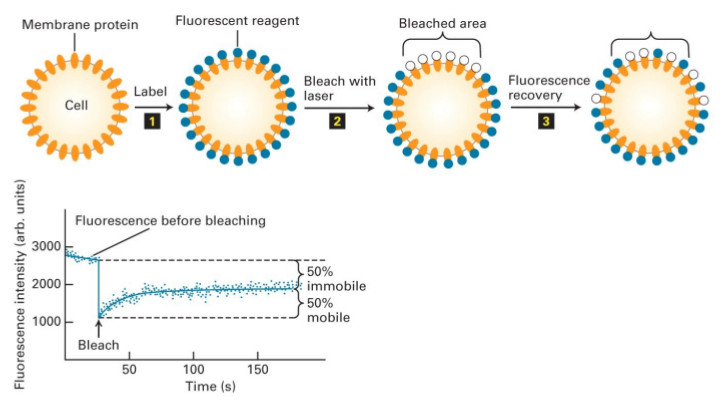
\includegraphics[scale=0.4]{immagine/frap.jpg}
\caption{Tecnica FRAP (fluorescence recovery after photobleaching)}
\end{figure}

Bombardando le molecole fluorescenti con un raggio laser molto intenso e per un certo tempo (fotobleaching), la molecola è incapace di rifare il ciclo di eccitazione, e si \emph{"acceca" o fotodecompone}, dopodiché non partecipa più al ciclo di eccitazione e dove era presente avremo una zona buia. Se misuriamo la fluorescenza in quella zona, o non ricompare o ricompare\footnote{Il photobleaching è irreversibile: una molecola accecata non può riprendere ad emettere}. Se la fluorescenza ricompare, ciò non può che derivare da un \emph{movimento di traslazione} delle proteine.

Se iniziamo con l'avere un certo segnale fluorescente sulla membrana e poi bleachamo in un punto, il segnale cessa di esistere nella zona bleachata ma si avrà poi un recupero della fluorescina che può essere completo: in tal caso mobilità 100\%, può però anche non avvenire assolutamente e in questo caso si parla di immobilità, o si può aver un intermedio, come nel nostro caso, in cui abbiamo un 50\% di mobilità.

Se ripetiamo questo su diverse proteine, scopriamo che proteine diverse hanno mobilità diversa, non solo, scopriamo anche che se noi trattiamo la matrice extracellulare o il citoscheletro con dei distruttori di legami, vediamo che proteine precedentemente poco mobili diventano molto più mobili, dimostrando crucialmente che sia la matrice extra cellulare, (che è una trama abbastanza strutturata), sia il citoscheletro (più strutturato), hanno dei legami importantissimi con le proteine.


Proteine diverse hanno mobilità diverse. Se trattiamo la matrice extracellulare o il citoscheletro con distruttori di legami, le proteine prima poco  mobili adesso lo sono molto di più: ciò dimostra  che sia la matrice extra cellulare, (che è una trama abbastanza strutturata), sia il citoscheletro (più strutturato), hanno dei legami importantissimi con le proteine.
L'importanza di questi legami è rilevante in alcune malattie: il complesso della \emph{distrofina} è importante per conferire al muscolo scheletrico la capacità di non strappare la membrana sotto sollecitazione meccanica. Tutto ciò è possibile se il complesso della distrofina è integro e lega da una parte la matrice e dall'altra il citoscheletro; quando è difettoso (di solito per problemi genetici) si hanno le distrofie muscolari, che progressivamente distruggono i muscoli tanto più quelli lavorano.

\subsubsection{Doppio strato lipidico}
Nel doppio strato, i fosfolipidi sono affiancati da altre molecole lipidiche: \emph{glicolipidi} (sfingomielina) e \emph{colesterolo}. 

\begin{figure}[H]
\centering
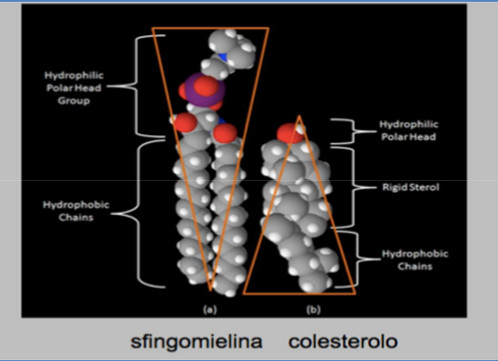
\includegraphics[scale=0.5]{immagine/sfingomielina.jpg}
\caption{Struttura di sfingomielina e colesterolo}
\end{figure}

Esse si inseriscono nella membrana in modi particolari: negli studi di biochimica, per estrarre proteine usiamo dei solubilizzanti della componente lipidica. Se li usiamo per dissociare le proteine dai lipidI vediamo che, utilizzando molecole meno aggressive, otteniamo una frazione proteica molto ricca, ma che porta con sé una grande quantità di lipidi, in particolare proprio colesterolo e sfingomielina: la  membrana è quindi organizzata in maniera \emph{discreta}. Le proteine sono aggregate in regioni speciali, o \emph{RAFT} (zattere). Questa idea nasce dal fatto che queste zone resistono alla dissociazione rispetto alle regioni non raft. Le strutture del RAFT sono interconnesse. Le RAFT sono mobili nell'intero doppio strato, a meno di ancoraggi citoscheletrici.

\emph{Perchè la struttura RAFT è importante?}

La suddivisione della membrana in zone raft e non raft ha a che fare con la funzione di \emph{comunicazione} delle membrane, perchè la limitazione data dalla velocità di diffusione libera pone un problema: se due molecole, A e B, devono interagire e si trovano ad una distanza variabile, prima di dare il prodotto servirà molto tempo, tanto più quanto è grande la loro distanza (relazione esponenziale).
Questo significa che un dispositivo senza zattere produrrebbe risposte variabili o addirittura impossibili. Quindi la limitazione che impone la diffusione esige che i prodotti vengano forniti quando i reagenti siano ad una distanza minima possibile.

Inoltre, una cellula quasi mai ha esigenza di comunicazione ed attività biochimica \emph{uniforme} in tutta la membrana.
\paragraph{Esempio: livelli di calcio}
In alcuni fenomeni cellulari è importante che si elevi transitoriamente la concentrazione di calcio intracellulare, come nei fenomeni secretori (ad esempio secrezione di neurotrasmettitori).
Se per innalzarne il livello nella cellula dovessimo tappezzare la membrana di canali adduttori di calcio, la cellula sarebbe facilmente esposta all'\emph{overload di calcio}\footnote{eccesso di Ca, che è tossico}.
È meglio collocare i canali calcio solo nelle zone in cui serve il calcio, mentre nel resto della membrana no.

\paragraph{}
L'organizzazione discreta della membrana riflette due esigenze:
\begin{enumerate}
\item{Continuità di gruppi funzionali}
\item{Regionalizzazione di funzioni diverse in zone diverse della stessa membrana}
\end{enumerate}

La membrana è organizzata in zone raft e non raft. Le zone raft si riconoscono perchè lì dove si verifica l'inserimento di lipidi speciali, esiste una quantità di molecole proteiche caratteristiche di queste zone, e funzionano come \emph{indirizzatori} delle varie proteine che fanno parte di uno specifico raft.

\emph{Il raft è quindi un centro di reclutamento di proteine devolute a funzioni associate}.

Ci sono 2 tipi di raft:
\begin{enumerate}
\item{Raft planare: le proteine prendono contatti con ormeggi citoscheletrici che assicurano questo l'ancoraggio è
dato da queste relazioni.}
\item{Raft invaginato: invaginazione (caveola) che presenta molecole proteiche particolari, le \emph{caveoline}, che inducono la piegatura}
\end{enumerate}

Le caveoline, per come legano le molecole, inducono una piegatura, quindi sono i \emph{sagomatori della caveola}. Se usiamo dei veleni che distruggono il citoscheletro, le caveole si liberano di questa forma incavata e divetano planari.
\begin{figure}[H]
\centering
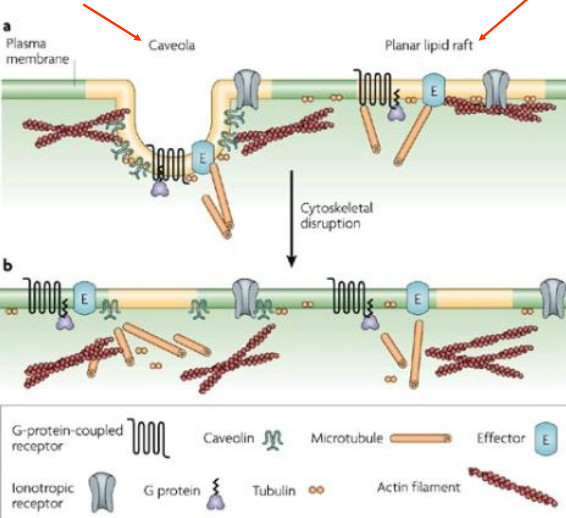
\includegraphics[scale=0.5]{immagine/raft1.jpg}
\caption{I due tipi di raft: invaginato (a) e planare (b), ottenuto dal trattamento dell'invaginato con veleni che distruggono il citoscheletro.}
\end{figure}
In che cosa una caveola può essere diversa funzionalmente da un raft lipidico planare? 

Le caveole possono essere di diversi ordini e possono anche essere degli incavi piuttosto estesi: quanto più si estendono, tanto più avremo delimitato uno spazio che diventa \emph{segregato}. Qui l'immissione di molecole ha un effetto diverso dall'immissione nel liquido extracellulare di una molecola prodotta nella cellula:a parità di molecole prodotte, avremmo un volume di soluzione che le accoglie diverso. Se la cellula secerne fuori da una caveola, l'elevazione della concentrazione sarà modesta; se immessa nella caveola invece, l'aumento della concentrazione sarà enorme. Viene quindi compartimentata la sostanza e si creano degli spazi confinati da cui sfuggire risulta difficoltoso.

Si fanno i conti con la diffusione: in uno spazio piccolo come la caveola è difficile che la diffusione faccia compiere movimenti indirizzati esclusivamente all'uscita; si crea così una concentrazione estremamente elevata di una sostanza al suo interno.

Ad esempio, i fenomeni autocrini in cui le cellule producono delle molecole e poi hanno i recettori per leggerli, non è un attività folle della cellula, in realtà le cellule fanno questo quando associano la produzione di qualcosa all'effettuarsi di certe risposte.


Nel terminale sinaptico, l'esocitosi del neurotrasmettitore viene associata alla secrezione di ATP: esso viene idrolizzato e l'adenosina collabora con i propri recettori. La cellula sta comunicando a se stessa l'entità del fenomeno di secrezione: quanto più è attivo il terminale sinaptico, tanto più ATP viene prodotto. Non stupisce che la risposta di questi recettori sia quella di depotenziare il processo di secrezione: questo diventa un sistema di \emph{autoregolazione}.

\paragraph{Signalplex}

Un raft è una buona base per costituire il \emph{signalplex}: è un \emph{complesso di segnalazione}. Quando analizziamo la funzione di comunicazione, il signalplex raggiunge il grado di aggregazione più alto: vi troviamo molecole con funzione ben definita, come canali ionici\footnote{funzione di fare transizioni conformazionali. Alcune conformazioni permettono il passaggio di ioni, altre lo impediscono}, enzimi. Essi, essendo modulabili, possono esplorare la membrana in varia maniera perchè ci sono modificazioni che ne modulano l'attività e la cinetica, e quindi la funzione. 

\begin{figure}[H]
\centering
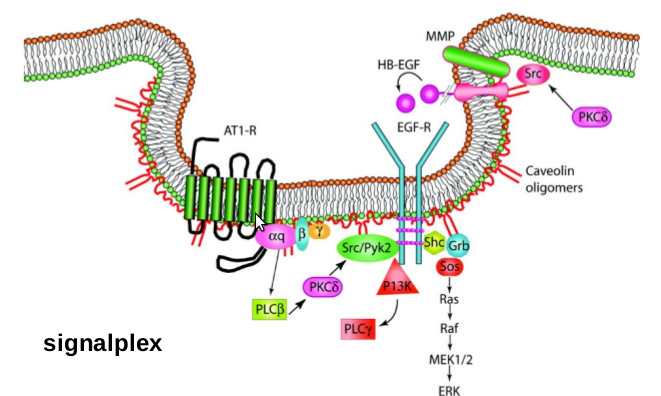
\includegraphics[scale=0.4]{immagine/plex.jpg}
\caption{Struttura di un signalplex}
\end{figure}

La molecola proteica sintetizzata potrebbe assumere molte conformazioni, in realtà poi i sistemi di ripiegatura ordinata ne determinano una certa struttura: attorno ad essa, i vari gruppi oscillano, si contraggono, si rilasciano. Tutti questi movimenti sono indotti dall'energia termica.
Ogni tanto il sistema, sollecitato in maniera vantaggiosa, cambia conformazione alterando o non la sua funzione ad esempio canale ionico aperto o chiuso o enzima respinge o no il sito al substrato.

Questa dinamica può essere descritta come se fosse un panorama collinare o montano in cui vediamo picchi e valli: i picchi significano energia libera maggiore e le valli minori. La proteina quindi si muove spinta dall'energia termica fra questi minimi, che sono più stabili. Un enzima o un canale ionico non hanno un modo unico di \emph{esplorare il panorama}, ma lo possono fare in diverse maniere perché ad esempio la fosforilazione, attaccando un fosfato su un residuo amminoacidico, li modifica.

In genere vengono selezionati processi di modificazione che influenzano una zona particolare di una proteina. Quando un certo gruppo si lega, il rispondere all'energia termica casuale fa attraversare prevalentemente certi minimi. Se i minimi sono associati o con l'aumento o con la diminuzione della funzione primaria, ecco che, attraverso questo, abbiamo modulato la cinetica e quindi la funzione della molecola.

Nel signalplex troviamo spesso recettori, canali ionici, delle chinasi associate (A, C). Il grado di complessità è elevato. Lo studio funzionale di regioni di membrana di questo tipo, tanto che si può studiare come sitema isolato una regiore ricca di molecole di segnalazione mettendole in una pipetta di vetro e portandole via dalla membrana. Negli eritrociti umani abbiamo canali per il potassio di tipo E-K: possiamo leggere la corrente in pA attravero la membrana modulabili attravero l'aggiunta di molecole che fosforilano/defosforilano i canali.

Un signalplex è l'ambiente ideale per far lavorare enzimi e molecole funzionali perchè risolve il problema della continuità e della regionalizzazione. Inoltre fa si che il grado di complessità funzionale che la molecola può esprimere, arrivi a massimo livello.

L'acquisizione di un'organizzazione di questo tipo è funzionale al \emph{realizzarsi di risposte variabili}: non avremo più uno stato zero e uno stato uno (funziona o non funziona) ma avremo dei livelli di funzionamento molteplici. In questo modo realizziamo una risposta complessa ed è ciò che distingue un sistema vivente da un sistema artificiale.

(14.10.14)
\section{Meccanismi di permeazione, canali ionici e trasportatori di membrana}

La membrana è regionalizzata in diverse aree, che posseggono specifici elementi molecolari proteici che determinano varie \emph{funzioni}, espresse da specifiche proteine funzionali : danno alla cellula la competenza a svolgere queste funzioni modulando tre attributi, qualità, densità e localizzazione delle molecole.

\paragraph{Qualità e densità}
una cellula è caratterizzata fenotipicamente dal fatto che esprime specifiche proteine funzionali.
Una cellula che risponde ad un ormone deve avere una competenza per esprimere molecole proteiche recettrici per quella determinata molecola segnale, inoltre la risposta sarà più o meno responsiva all’ormone a seconda della densità delle molecole recettrici piazzate sulla membrana. Non ci stupirà sapere quindi che la sensibilità ad un certo ormone può essere modulata mediante la sintesi di un numero cospicuo o meno di recettori. 


\paragraph{Localizzazione} fa sì che una cellula abbia una sensibilità particolare a certi stimoli in regioni particolari della membrana. Oltre ad avere un fenotipo generico, essa può avere dunque regioni specializzate per svolgere determinate funzioni. L'esempio tipico è quello di una cellula neuronale: essa esprime al massimo grado il differenziamento regionale, essendo la regione dei terminali diversa per funzioni rispetto al colletto assonico ed ad altre porzioni, come il dendrite.
Il fenotipo nervoso esprimerà una certa quantità di proteine funzionali e inoltre la loro localizzazione specifica in determinate regioni fa sì che il dendrite sia un apparato di recezione, il colletto assonico sia un punto decisionale che decide se la cellula sarà eccitata o no e il teminale sinaptico sia un effettore, perché in grado di produrre un effetto, ovvero il rilascio del neurotrasmettitore per creare uno stimolo che passerà alla cellula contigua.


\subsection{Trasporti transepiteliali}
Le barriere sono di diversa natura: più o meno selettive, ad esempio come un epitelio (sistema renale, sistema gastroenterico) e a giunzioni strette, le quali impediscono il passaggio di soluti tra cellula e cellula.

Queste cellule normalmente si interfacciano con un fluido extracellulare ed un capillare, caratterizzato da un \emph{endotelio non serrato}, ma lasso, che permette porosità più o meno ampie tra cellula e cellula delimitante. Mentre i soluti potranno passare per flusso di massa (acqua più tutti i soluti, senza distinzione o selettività), il passaggio di soluti attraverso l’epitelio stretto non avviene così.

Attraverso l'  \emph{epitelio stretto}, il flusso intercellulare è impedito dalle giunzioni strette e l’unica possibilità di una sostanza per passare è quella di attraversare la barriera costituita dalla membrana plasmatica.

La membrana plasmatica consta di due porzioni: la prima è quella \emph{fosfolipidica} che è a sua volta una barriera, perché selettiva, la seconda è costituita da alcune \emph{formazioni molecolari proteiche} che si organizzano a canale o a trasportatore e che permettono un passaggio di tipo diverso da quello lipidico.
Affrontare il problema della permeazione attraverso la membrana significa trattare due cose distinte: il passaggio di alcuni soluti attraverso il doppio strato lipidico e il passaggio di altri attraverso delle strutture proteiche.


\paragraph{Come si comportano le sostanze nei confronti del doppio strato lipidico?}
\begin{itemize}
\item{Gas di interesse respiratorio: $CO_{2}$, $N_{2}$, $0_{2}$ passano il doppio strato lipidico}
\item{Piccole molecole polari non cariche : (urea, etanolo) passano il doppio strato}
\item{$H_{2}O$ : incapace di passare se non in quantità irrilevanti}
\item{Molecole grandi polari non cariche : glucosio, non passano}
\item{Sostanze cariche (ioni): non passano}
\item{Molecole polari non cariche (aa): non passano}
\end{itemize}

I trasporti transmembranari si distinguono in:
\begin{itemize}
\item{In forma libera: per le molecole che diffondono nel doppio strato}
\item{Tramite proteine transmembranarie: per le altre molecole}
\end{itemize}
\begin{figure}[H]
\centering
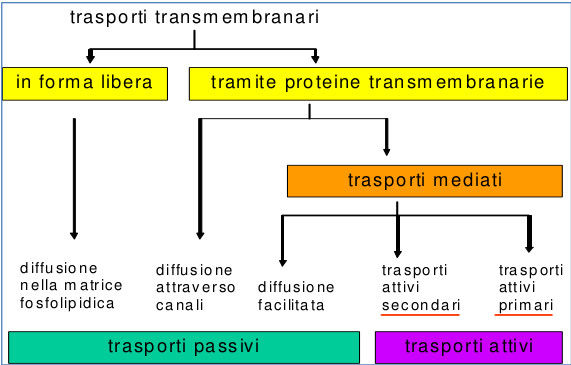
\includegraphics[scale=0.5]{immagine/riepilogo.jpg}
\caption{Trasporti transmembranari}
\end{figure}

Tutti i trasporti necessitano di energia sotto forma di \emph{gradiente} (trasporto passivo): quelli che hanno bisogno di energia spesa dalla cellula, spendono energia metabolica. Il gradiente è a spesa energetica nulla per la cellula.

\subsection{Proteine transmembranarie}
Un passaggio che impiega una proteina ma non implica spesa di energia è la \emph{diffusione attraverso canali}.
Gli ioni ad esempio hanno una via preferenziale costituita dai canali ionici. Questi, permettono il passaggio di ioni utilizzando il potenziale elettrochimico (in quanto molecole cariche).

I trasporti mediati sono trasporti in cui la molecola proteica funziona da \emph{trasportatore}.
Abbiamo poi i trasporti attivo primario e secondario, che avvengono fino a che la cellula può idrolizzare ATP; nel momento in cui avveleniamo la cellula essa non farà
più questi due tipi di trasporto.

I primari sono mediati da molecole proteiche, pompe, che direttamente idrolizzano ATP (ATPasi) e permettono il passaggio di ioni in maniera congiunta. 

I secondari non utilizzano direttamente ATP, ma vengono utilizzati i gradienti costruiti dalle pompe per accoppiare altri trasporti.

Ad esempio, se la pompa sodio potassio mantiene un gradiente in cui il sodio viene estruso e il potassio viene rimesso in cellula, un’altra molecola può usare questo gradiente per accoppiare un trasporto. Le seconde utilizzano dunque il risultato delle prime. Perché si usa questo termine che può confondere? Perché li chiamiamo attivi lo stesso? Entrambi appaiono attivi perché se noi blocchiamo l’ATP entrambi si bloccano.

\subsection{Diffusione libera}
Attraverso il doppio strato: determiniamo la concentrazione nel mezzo acquoso della sostanza di interesse per la diffusione (nella fase oleosa non si può misurare la concentrazione).
Quello che possiamo determinare in una situazione del genere, è la concentrazione nel mezzo acquoso della sostanza di cui vogliamo studiare la permeazione.
Ci troviamo di fronte ad un passaggio di fase: acquosa-oleosa, oleosa-acquosa e abbiamo uno spessore. È un problema applicare la legge di Fick, perchè si applica al mezzo acquoso : possiamo però calcolare la concentrazione nel mezzo acquoso e poi ricavarci quella nel mezzo oleoso\footnote{quella che interessa a noi}, tramite il \emph{coefficiente di ripartizione}: si usa un pallone di separazione, che separa i lipidi dal mezzo acquoso, si mette la molecola della quale si vuole stabilire il coefficiente di ripartizione, si agita e attendiamo: si ha \emph{separazione della fase} e parte della molecola sarà in quella oleosa, parte in quella acquosa. Si preleva prima una fase, poi l'altra, si analizza il contenuto e a parità di concentraizone di partenza possiamo vedere la frazione che sta nella parte oleosa e quella nella fase acquosa, tramite il coefficiente di ripartizione, definito come:
		\begin{equation}
		\centering
				K =\frac{C^{m}}{C^{aq}}  
		\end{equation}		
				  
dove $C^{m}$ è la concentrazione nella fase oleosa e $C^{aq}$ la concentrazione nella fase acquosa.
K indica la frazione di molecole che troviamo nella parte oleosa rispetto a quelle nella parte acquosa. Se la molecola si distribuisce egualmente la K è uguale a 0,5. Se invece è poco liposolubile avremo 1/10: 9 parti all’acquosa e 1 parte all’oleosa.

Sapendo ciò, riscriviamo l'eq di Fick corretta:
\begin{equation}
\centering
\frac{dn}{dt} = \frac{KD}{x} A(C^{aq}_{1} - C^{aq}_{2})
\end{equation}

e definiamo $P = \frac{KD}{x}$ il coefficiente di permeabilità.
Questo ci permette di concludere che se vogliamo stabilire il flusso di una sostanza che passa il doppio strato, co-
noscendo la sua mobilità, tabulata, e conoscendo la concentrazione delle due fasi acquosa (stabilita da noi in laboratorio) e oleosa, non possiamo esprimere tutto in termini di legge di Fick se non la correggiamo prima
col coefficiente di ripartizione. Per un saggio quindi dobbiamo fare riferimento anche alle concentrazioni nella
fase oleosa.

Possiamo correlare quindi il fatto che una sostanza passi meglio o peggio attraverso la membrana o se è più grande o più piccola con il fatto che abbia maggiore o minore coefficiente di ripartizione.

Se vogliamo calcolare il flusso, si stabilisce una certa differenza di concentrazione e si valuta il flusso per unità di salto di concentrazione. Il coefficiente di permeabilità è quindi una caratteristica di una barriera che possiamo sperimentalmente determinare.
\begin{equation}
\centering
J = P \Delta C
\end{equation}

Se misuriamo il P di diverse molecole che differiscono per la costante D o per K coefficiente di ripartizione, e le mettiamo in correlazione con K\footnote{correlare due paramentri significa stabilire quanto i due parametri interdipendono tra loro}: 
\begin{figure}[H]
\centering
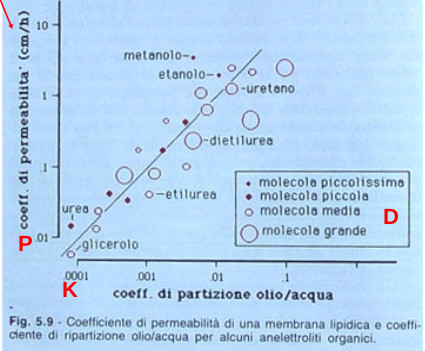
\includegraphics[scale=0.5]{immagine/ripartizione.jpg}
\caption{Grafico di P in funzione di K}
\end{figure}

Si possono avere 3 casi:
\begin{enumerate}
\item{Grafico x/y in cui non c'è correlazione. I punti sono dispersi e K=0}
\item{Grafico x/y in cui c’è parziale correlazione. I punti si avvicinano ad una retta ma senza sovrapporvisi. 0<K<1}
\item{Grafico x/y in cui c’è correlazione totale. I punti sono su una retta in modo preciso. K=1 o K=-1}
\end{enumerate} 

I punti possono anche orientarsi su una retta decrescente : si ha alta correlazione inversa. Le varie sostanze si allineano perfettamente facendo una correlazione KP alla retta di regressione = -1.

La più importante caratteristica di una molecola di soluto perché possa essere permeata attraverso il doppio strato lipidico è il suo \emph{coefficiente di ripartizione}. Tanto più si ripartisce bene nei lipidi (o tanto più è liposolubile) tanto più passa bene.
Molecole grandi e piccole le troviamo in egual modo con alta permeabilità e con bassa permeabilità. Pesa pochissimo, per la bontà del passaggio attraverso la membrana, l'ingombro e la costante di diffusione D, ma pesa moltissimo la liposolubilità o coefficiente di ripartizione.

\subsection{Canali e trasportatori}
Distinguiamo due tipi di molecole: canali e trasportatori (entrambe attivi).

Il \emph{Canale ionico} è un edificio molecolare che stabilisce un canale acquoso persistente. La membrana è forellata da questi canali che contengono acqua, la separano dal doppio strato: l'acqua ha una seconda modalità di passare, che è fisiologicamente rilevante. 

Il \emph{trasportatore} è un edificio molecolare proteico che non sagoma un poro, ma può attraverso cambi conformazionale, prendere contatto, esporre una parte interna alternativamente alla faccia esterna o a quella interna della membrana.
Es, membrana con un canale e due tipi di trasportatore, e supponiamo di poterli attivare alternativamente: mettiamo un elettrodo da una parte della membrana e uno dall'altra, e facciamo passare la corrente: se attiviamo i canali ionici, la corrente passerà, se invece attiviamo i trasportatori la corrente non passerà. Nel canale ionico quindi possono passare cariche da una parte all'altra, nel trasportatore no: tuttavia, i canali possono esistere in conformazioni diverse perchè possono sagomarsi in modo da lasciar passare ioni o in modo da NON lasciarli passare: si parla di CANALI APERTI e CANALI CHIUSI. Se il canale è inattivo, è chiuso. Se è attivo (come descritto prima), è aperto.

I trasportatori possono trasportare da $10^{2}$ a $10^{4}$ molecole per secondo.
Una pompa ionica  (trasportatore pimario) va da 10 a 1000 ioni per secondo.
I canali ionici da $10^{7}$ a $10^{8}$ ioni al secondo.

I TRASPORTATORI possono essre:
1. semplici
2. accoppiati nella stesas direzione
3. accoppiati nella direzione opposta.

Come le molecole proteiche possono svolgere funzioni associate alla onformazione della molecola?
Le conformazioni possono essere più o meno stabili: minore è l'energia libera, più è stabile la conformazione (vedi slides grafici): la probabilità di soggiornare in un minimo energetico dipende dall'energia di attivazione pr passare all'altra conformazione.
Come descriviamo il panorama energetico di una molecola proteica?
PIcchi e minimi: l'agitazione termica sposta la molecola proteica tra i vari minimi. Una proteina ha uno schema cinetico di funzionamento, visitando in tempi diversi divrsi minimi. Se è una molecola di trasporto, come una canale ionico, può essere in due conformazione: chiusa o aperta. Cosa fa aprire/chiudere i canali? La differenza di potenziale non apre/chiude i  canali, ma aumenta/diminuisce la probabilità della molecola di trovarsi in uno dei due minimi che corrispondono alla situazine chiuso/aperto. Ciò che regola apertura è chiusiura è l'AGITAZIONE TERMICA. 
Se alla molecola attacco un fosfato, il panorama cambia: impongo alla molecola un nuovo minimo.

Quando un soluto lega il sito della proteina, transitoriamente farà parte della molecola proteica --> interferisce nel panorama energetico, e può determinare un cambio conformazionale (ciò che accade nei trasportatori): ciò può determinare anche un cambio di affinità con un certo soluto.
L'accesso del soluto nel trasportatore può avvenire da entrambe le facce della membrana.

Trasportatori: uniporto, simporto e antiporto.
Canali: passivi, voltaggio attivati, chimmicamente attivati, meccanidamente attivati. tutti i canali ionici sono di questi quattro tipi (es i fotoni determinano un'attivazione chimica).

Anche se una membrana non viene stimolata, la permeabilità deve essere garantita: ciò è ad opera dei canali PASSIVI.

I TRASPORTI MEDIATI hanno caratterestiche:
- specificità : la molecola trasportata è compatibile con il sito recettoriale della molecola trasortatrice. Passano unicamente attraverso quel veicolo le molecole fatte in un certo modo. Ci osno i canali più o meno specifici.
- saturazione :  data la bassa efficienza dei trasportatori, trasportanto tante più molecole quanto più è alta la loro concentrazione. Se saturiamo, ad un certo punto tutto si blocca.
- competizione : se abbiamo molecole che riconoscono il sito del trasportatore, queste verranno trasportate al posto della specie di riferimento. Possiamo avere un'inibizione del trasoprto per via competitiva o ...?

DIFFUSIONE FACILITATA
due conformazioni della moelcola trasportatrice: T1 e T2
Se il glucosio è presente, lega la molecola e impone un cambio di conformazione (T2). Quando viene rilasciato, si ha di nuovo la conformazioe iniziale T1. Siffatto sistema funziona dominato dal salto di concentrazione: se cambio il gradiente, il trasporto si inverte.
Sono molecole che hanno un gran numero di alpha-eliche (es GLUT-1) e che devono essere inserite nel modo corretto nella membrana. In genenre delimitano uno spazio interno, che non è un canale ionico, ma una struttura capace di presentare una regione cava che può essere esposta sulle due facce. La FLORETINA è un famraco che blocca il legame alla molecola segnale.
Il lucosio rappresenta anche, per alcune cellule come le neuronali (a cui si riferisce la curva superiore) o le cellule del pancreas (inferiore):
La relazione tra glicemia e flusso attraverso il trasportatore, entrambe le curve crescono al crescere della molecola, e tendono a saturare, ma nel neurone, che deve solo utilizzare il glucosio, nella concentraizoen in cui la glicemia oscilla, c'è già un plateau ---> se i lglucosio cresce o meno nel plasma, il neurone prende e basta, non segnala; nelle cellule del pancreas si ha invece variazione di captazione che risente della concentraizone del glucosio nel plasma.
Entrmabe le cellule hanno GLUT1, ma la densità di questi e la localizzazion fanno si che la diffusione differisca.

Se la molecola trasortatrice fa variare anche l'affinità oltre alla concentrazione, la struttura avrà un comportamento più sofisticato:
- Pompe
- trasporti attivi secondari.
Differiscono dalla diffusione facilitata proprio perchè oltre alla concentrazione fanno variare l'affinità.
il ligando lega il sito recettoriale secondo una Kd. Mentre in un trasporto mediato semplice la concentrazione intracellulare non ecced equella extracellulare, in questo tipo di trasporto la concentrazione puiò essere più alta all'esterno.

- TRASPORTO ATTIVO SECONDARIO: SGLUT1 (sodio-glucosio trasportatore), coopera con il gradiente di Na oltre che con quello di glucosio; se bassa [glucosio] all'esterno e alta di Na (pompa na-K), la molecola utilizza questo gradiente di Na creato spendendo ATp da parte della poma primaria. Na si lega e crea un sito di legame per il glucosio: legame glucosio, poi cambio conformazionale e rilascio delle due molecole nel lume cellulare. (COTRASPORTO)
L'energia viene da:
- idrolisi ATp delle pompe
- pot elettrochimico del Na 

-POMPE IONICHE (TRASPORTI ATTIVI PRIMARI): hanno due domini, uno catalitico (ATPasi) e uno di trasporto.
Classe V e classe F --> pompe protoniche
Classe P ---> pompe ioniche
4 subunità, due alpha e due beta. Abbiao due conformazioni, E1 ed E2.
Es. POMPA Na/K (classe P)
E1 : abbiamo l'ATP legato alla molecola e i siti per il sodio esposti intermìnamente; tre Na si legano e questo facilita la fosforilazione, che cambia la conformaione e l'affinità della molecola, per cui passiamo alla configurazione E2.
E2 : Na rilasciato e legamo del K, che induce la defosforilaizone, e si torna ad E1.
N.B. non è generale!!
Questa pompa, spendendo ATP, crea un gradiente alettrochimico per Na e K. Crea inoltre:
- Elettrogenesi: se andiamo a vedere quanto Na e K sono spostati, 3 Na vengono estrusi contro 2 K ---> potenziale di membrna, piccolo ma significativo.
- Ipotonicità: sposta sodio ed immette meno potassio

POMPE CALCIO
Sono ATPasi che spostano solo calcio. 2 tipologie:
- PMCA :associate a membana. Spostano Ca dal citosol al liquido extracellulare
- SERCA : associate al RE, catturano Ca citosolico all'interno del lume del RE. Il RE è un DEPOSITO di calcio, perchè sia sulla membrana plasmatica che sulla membrana del reticol oabbiamo canali ionici pr il Ca che, se aperti, producono l'influsso di calcio (da fuori verso la membrana) o il rilascio (dal reticolo verso il citosol). 
Il Ca ha il ruolo di messaggero intracellulare \lfreccia ecco perchè è mantenuto  concentraizone molto bassa fiuori dal RE.

POLARIZZAZIONE DEI SISTEMI DI TRASPORTO
Es cellule ossintiche nell'organo gastrico, responsabili della produzione di HCl: c'è un apompa protonica sulla membrana luminare (che vede il lume gastrico) per il K, poi due trasportatori, uno sulla membrana baso-laterale e uno sulla luminare per il Cl.

Il passaggio privilegiato dell'acqua avviene attraverso canali speciali, le ACQUAPORINE, caratterizzati da sequenze di Ans, Pro, Ala. Le molecole di acqua passano ruotando in maniera particolare: l'asse cambia orientamento e così riescono a passare con moltissima efficienza. Non possono passare altri ioni!
Esperimento. ovpociti di rana con e senza acquaporine: con, l'acqua entra e la forma si scompone perchè non c'è omogeneità nella struttura citoscheletrica.

(15.10.2014)

PROTEIN TAGETING E TRAFFITING
Traffiting \lfreccia traffico nella cellula delle molecole proteiche
Targeting \lfreccia raggiungere target ben precisi.

Circa 20000 proteine vengono prodote da una cellula e sono l'espressione del fenotipo cellulare. Vengon prodotte in:
- Mitocondri : ecco perchè alcune malattie genetiche hanno divrsa incidenza se si considera la provenienza materna o paterna;
- Ribosomi liberi
- ribosomi associati al RE : vengono prodotte più che altro proteine secretorie e integrali di membrana.
Specificità del sito di sintesi dipende dalla natura della proteina.
Nel sistema di sintesi nei ribosomi liberi, la lettura dell'mRNa sui traduce in un polipeptide immesso direttamente nel citosol; solo dopo che è stato tradotto, le rpoteine vengon inserite negli organelli.
Nei ribosomi associati al RE, la produzione del polipeptide avviene all'interno del lume del RE, in una modalità legata alla membrana plasmatica \lfreccia importazione cotraslazionale: traduzione ed inserimento nel doppio strato sono simultanei.

Nel doppio strato troviamo le alpha-eliche: il peptide può essere gran parte all'esterno o all'interno, e il dominio carbossi all'interno o all'esterno \lfreccia INSERIMENTO VETTORIALE: spesso le regioni terminali ammino/carbossi hanno funzione ben precisa nella proteina ed è importante che stiano dove devono stare (all'interno o all'esterno).
Come fanno proteine diverse ad essere orientante diversamente nella membrna?
L'inserimento se lo portano dietro per tutte le fasi successive a quella dell'inserimento nello strato lipidico e traduzione.

PROTEINE SECRETORIE: 
Esiston ocomplessi SRP (riconoscimento segnale) che riconoscono la regione iniziale amminica del polipeptide; anche recettori sulla membrana el RE risconoscono SRP.
nell'interno del lume esistono gli chaperoni, che assistono il folding.

Es. Insulina: eliminata la prima parte segnale, proteina svolta all'interno fino all'incontro di una sequenza di stop, un'alpha-elica, a partire dalla quale il resto del peptide viene svolto all'esterno.

Es. asialoglicoproteina: la prima sequenza segnale viene mantenuta, la proteina viene svolta fino alla sequenza di stop, poi svolta all'interno-

Es. Citocromo P450: sequenza stop molto precoce, protenina tutta nel citosol.
Es. Glucosio strasportatore: molte alpha-eliche transmembrana. L'alpha elica cambia l'oroentamento dello svolgimento della proteina.

La tipologia di proteine tradotte condiziona il posizionamento dlele alpha-eliche. È importante stabilire la posizione in fase di sintesi, perchè poi l'orientamento viene mantenuto. (vescicole ???)
qualsiasi membrana interna può fare invaginazione:
- pinocitosi : curvature della membrana che si creano perchè si realizzano forze di trazione a partire dal citoscheletro. La vesciocola contiene tutto il liquido extracellulare. Usato per la veicolazione dei farmaci.
- endocitosi indotta da recettore : il ligando recluta molecole come la clatrina, si forma una vescicola rivestita di clatrina: essa dà la curvatura alla vescicola (sistema più specifico). La cellula sceglie il cargo da importare: le proteine che riconoscono le molecole saranno incluse nell'invaginazione. Due livelli di decisione:
1. recettore
2. molecole da internalizzare

Processo opposto è la GEMMAZIONE: la membnrana estroflette. Ci sono sempre molecole specifiche (recettori cargo, adattine). Dopo l'involucro viene perso ---> vescicole NUDE che vagano per la cellula.

Una vescicola può rifondersi con una membrana: 
- Attracco : la vescicola porta molecole rpoteiche precise che sono GTPasi Rab e le V-SNARE.
- Ormeggio
- Fusione

Le GTPasi sono di due tipi: monomeriche e trimeriche.
1. GTPasi TRIMERICHE: ho un recettore con legata una proteina alpha-beta-gamma. Il legame del GTP permette il distacco di una subunità che va ad agire su un'enzima (es Adenilati ciclasi) e produrrà una certa sostanza (in questo caso, il cAMP).
2. GTPasi MONOMERICHE: legano GTP, se attivate, e producono un effeto spesso legato all'attivaizone di una chinasi 8o di un enzima in generale). Tipiche sono la famiglia RAS (proliferaizone cellualre), Rho Racn (controllo citoscheletro)e Rab (regolatore del traffico vescicolare). A cascata attivano il processo a valle.

La vescicola presenta questa Rab che, se attivata, attiva la "proteina di attracco", o EFFETTORE DI RAB. L'ormeggio prevede l'attivazione dell T-SNARE, che levano le V-SNARE. Poi, per processi Ca-dipendenti, abbiamo una fusione della vescicola ormeggiata (il contenuto viene rilasciato).
QUesti processi di esocitosi avvengono in congiunzione con l'endocitosi per mantenere le dimensioni cellulari e l'omeostasi.

Ci sono dei GEF, fattori proteici che dipendono dai Rab e inducono l'attivaizone di Rab; Rab attiva la chinasi, che recluta effettori rab e proteine filamentose ---> assemblaggio di molti elementi proteici.
Prendendo due organelli, possiamo avere gemmazione in un organenllo e attracco nell'altro ---> trasferimento dei cargo da un lume ad un altro ---> TRAFFICO VESCICOLARE.
Il traffico vescicolare genera i processi di comunicazione intracellulare:
1. funzione secretoria : molecole sintetizzate nel RE trasferite al AG e poi alla membrana
2. Via endocitica : dalla membrana all'interno. Le impalcature proteiche possono subire danni da parte di radicali.

Il Golgi ospita un'inizio di glicosilazione ---> da proteina a GLICOPROTEINA (vedi citologia). C'è una selezione intelligente delle proteine cargo!
Ogni proteina ha un traffico TIPICO: la proteina subisce queste traslocazioni dopo essere stat aimmessa nella membrana: o viene reimmessa, o rimpiazzata. 
Esiste un pool di molecole mantenute in posizione sottomembranale: es canali per il calcio TRP che, se inseriti in memnbrana, la rendono permeabile al calcio. Devono essere pochi! I TRP vengo assunti per un scopo, ad esempio stimolaizione da parte di un fattore di crescita, poi eliminati: è un meccanismo di segnalazione estremamente localizzato in prossimità del recettore attivato dal ligando specifico, e può elevare la densità dei canali molto repentinamente ---> competenza spaziale e temporale ben contingentata. 

(21-10-14)

Prendiamo in esame la matrice extracellulare e il citoscheletro.
Lo spazio extracellulare è strutturato grazie alle interazioni tra molecole proteiche di membrana e molecole proteiche libere nella MEC (Esso rappresenta un pool di molecole di adesione che si ancorano a integrine).
Le integrino collegano la MEC al citoscheletro.

L'impalcatura creata fa in modo dissipare la forza dei movimenti della cellula, non scaricandola tutta sulla membrana.

CITOSCHELETRO.
L'agitazione termica determina i movimenti dei componenti cellulari sul citoscheletro.
Esso è un'intelaiatura meccanica che conferisce la forma alla cellula.

Funzione di ancoraggio
Esempio cellula neuronale: esso avrà citoscheletro caratterizzato da proteine di adesione specifiche per certe altre proteine di membrana. In particolari regioni della cellula devono trovare la loro locazione proteine specifiche, nonostante siano state sintetizzate nello stesso compartimento.
Passaggio dei globuli rossi nei capillari. Essi passano in singola fila e vengono deformati nei capillari della milza. I globuli rossi performanti resistono alla tensione meccanica, quelli vecchi invece collassano.
Le cellule riescono a sopportare deformazioni. Ciò è dovuto al citoscheletro corticale che prende interazioni particolari con proteine di membrana e proteine libere che formano nel complesso tensiostrutture.
Le tensiostrutture distribuiscono sollecitazioni meccaniche con un gradiente su tutta la struttura.

Visualizzazione citoscheletro. Esso è formato da tre aggregazioni proteiche: filamenti intermedi, microfilamenti e microtubuli.
Si usano anticorpi coniugati con composti fluorescenti in modo da visualizzare un componente. Possiamo inoltre utilizzare diversi fluorocromi che rispondono a una stessa lunghezze d'onda per visualizzare contemporaneamente le tre componenti.

ACTINA. Struttura. Costituiscono fibre da stress. 


Sollecitazione fibroblasto. Marchiamo l'actina. Essa è organizzata in fibre che vanno ad identificare le linee di forza a cui è sottoposta la cellula.
Cellule in coltura su un tappetino elastico disposte in modo random. Tiriamo il tappetino in due direzioni lungo una retta ed osserviamo che le fibre, nonché le cellule, si dispongono lungo la linea di tensione. Se cambiamo lo stimolo le cellule cambiano orientamento.
Adesioni focali. In esse è presente la vinculina che sono collegate con le fibre da stress.


TUBULINA. Struttura. Dimensione. Locazione.
Tutta la cellula è percorsa da questi binari su cui si trovano dei motori capaci di traslocare strutture interne. Esempio del fuso mitotico.

FILAMENTI SECONDARI. Dimensione. Strutture.
Sono gli elementi che connettono i tubuli a componenti strutturali ad esempio.

Il citoscheletro ci rimanda alla dinamica. Il citoscheletro è specializzatissimo nel movimento. Tutti i componenti del citoscheletro vanno incontro a fenomeni di polimerizzazione e depolimerizzazione in concomitanza alla spesa di energia ATP o GTP. La polimerizzazione è facilitata quando si raggiunge un'aggregazione di almeno 3 molecole proteiche. 
Fase di latenza. Fase di crescita molto veloce che inizia con la formazione dei trimeri. Fase di equilibrio. A questo punto l'addizione del l'actina globulare dipende dalla concentrazione residua.

L'aggiunta ha un sito preferenziale in cui non è necessario un cambio conformazionale del filamento per l'attacco. Sono distinte estremità più e meno.

Un altro fenomeno a cui sono soggetti i filamenti esalta la differenza tra le estremità.
In vitro. A concentrazioni minori di 0,6 avremo aggiunta maggiore di subunità all'estremità più. Il polimero crea un mulinello per cui si sposta la struttura a monte di un residuo marcato al tempo zero.
Un filamento si accresce o decresce nelle due direzioni possibili a diverse velocità. La dinamica molecolare della cellula è legata ai fenomeni di polimerizzazione e depolimerizzazione.

In vivo. Abbiamo cicli di velocizzazione dati da cofilina, profilina e timosina. La loro attività spiega la differenza di velocità dei fenomeni di polimerizzazione dei filamenti in vitro e in vivo.


Proteine accessorie si legano al citoscheletro e permettono la diversificazione delle forme cellulari mediante l'associazione in particolari conformazioni. 
Le proteine accessorie determinano una organizzazione sopra molecolare del polimero.
Si formano reti, fasci etc..

Motori molecolari o proteine capaci di cinetica.
MIOSINE classificate. Quelle di classe 2 la troviamo nei filamenti spesso del muscolo.
Quelle di classe 1 le troviamo con funzione di ATPasi a collegare, durante la contrazione del muscolo, l'actina. Quelle di classe 5 si trovano a collegare le vescicole permettendone la migrazione.
Nella muscolo, la cinetica della miosina avviene con attacco (movimento) cambio e distacco. La cinetica della miosina per lo spostamento delle vescicole avviene invece per attacco e movimento continuo senza distacco completo.


 Trappola ottica. Illuminiamo una sferetta con un raggio laser intrappolandola al centro del fuoco. Più è forte l'energia del laser, più si intrappola bene.
 Se sollecito la sferetta a muoversi, essa di muoverà in proporzione all'intensità del raggio. 
 Situazione in figura in alto a sinistra.
 Ogni volta che la miosina crea un colpo, le palline si sposteranno insieme alll'actina. Come? La miosina del muscolo tira e rilascia e il movimento appare in figura a destra in alto. La miosina di movimento delle vescicole invece non rilascia ma si sposta insieme all'actina mantenendo le sue due teste teste attaccate in modo alternato.


Riguardati la parte dei microtubili 


I MT costituiscono dei binari. L'estremità più va in periferia e la meno verso il centro di organizzazione. Si distinguono il percorso centrifugo e centrifugo.

Chinesine vanno verso più e le dineina verso meno secondo lo stesso schema di movimento.

Slide.
In termini elettrici il nostro organismo è costituito da soluzioni con molecole cariche e non cariche. 
Def. conduttori primari (elettroni portatori di carica e corrente)Def. corrente. Def. conduttori secondari (ioni portatori di carica e corrente).
Gli ioni possono passare con flusso di massa, ovvero liberamente, oppure possono passare selettivamente, attraverso una membrana a patto che ci siano i propri specifici canali. Inoltre uno ione può rimanere fermo su uno dei due lati della membrana.
Ogni compartimento è isopotenziale perché gli ioni vi si distribuiscono in modo omogeneo. Se noi vogliamo creare una differenza di potenziale, ovvero separare cariche, dovremmo spendere energia.
Ora ragioniamo tra due compartimenti. La membrana rappresenta due elementi circuitari: RESISTENZA, conduttore che ci dà facilità o difficoltà della corrente di attraversarlo, nel nostro caso sono i canali ionici. , CONDENSATORI: la matrice lipidica la rappresenta perché impedisce alla cariche di passare.

Slide.
Nel "punto di congiunzione" delle code dei fosfolipidi si ha il punto più debole in cui è possibile separare i due foglietti della membrana. Freeze-fracture. 
Lo spessore della membrana senza raft è di 5 nanometri. Qual'è il valore di capacità che rappresenta? Quante cariche può trattenere? Abbiamo la formula in figura. Epsilon è la costante dielettrica dei lipidi.
Ripassiamo un po' di fisica. Ceramica conduttiva fabbricata in modo da essere più o meno resistente. Il conduttore è ideale è fatto di rame.
 Nelle resistenze in serie, la resistenza totale è la somma delle resistenze.
 Nelle resistenze in parallelo, la G conduttanza, reciproco della resistenza, è la somma delle G delle singole resistenze.
 A naso, le resistenze in parallelo hanno più permissività di passaggio di cariche.
Esempio numerico.
Se nella membrana abbiamo diversi canali ionici, sarà più facile far passare corrente nella membrana. La membrana aumenta la sua conduttanza significa che aprirà i suoi canali ionici.

Leggi di kirchoff. 
Sx. Ho una batteria. Le cariche positive fluiscono. La corrente va dal polo più al polo meno ed è il flusso di cariche per secondo. Se entra in A, quello che esce deve essere uguale a quello che entra: corrente in A uguale a corrente in B.
Dx. Il voltaggio totale deve essere uguale alla somma dei voltaggi in 1 ed in 2.

(22.10.2014)
(la parte delle membrana non va fatta sul silverthorn!)
Precisazioni:
la membrana può essere considerata come un circuito resistenza-capacità in parallelo: applicando una ddp ai due capi, abbiamo flusso di ioni. Quali problemi ci sono?

1. Metodo di registrazione e visualizzazione dei segnali che vogliamo derivare. Questi segnali sono di bassa intensità (max 100mV) ed estreammente rapidi nel variare (anche 2msecondi). Serve un sistema che amplifichi la durata ddel sengale(?)
2. Non possiamo usare i sistemi classici come l'amperometro; serve un sistema che possa captare questi segnali, ovvero che utilizzi un ago magnetico che non ha inerzia \freccia OSCILLOMETRO: raggio elettronico (pennello elettronico) che può essere deviato da campi elettrici. Al contrario del sistema meccanico non ha inerzia. Tuboo di vetro con un catodo che viene riscaldato e, per effetto termoionico, emette elettroni; gli elettroni sono accelerati da un anodo e protiettati puntiformi sullo schermo anteriore. Lo schermo è trattato cn materiale luminescnete: quando gli elettroni impattano, creano un punto luminoso.
Il pennello elettronico può essere deflesso con due piastre che possono essere caricate, una + e una meno: gli elettron vanno verso la più e poi tornano indietro.
Per la dimensione temporale, usiamo due placche tra le quali applichiamo un segnale \emph{a dente di sega}. In questo modo osserviamo che il raggio va da sinistra verso destra. Per percorrere tutto quanto lo schermo, questo segnlae a dente di sega impiega un certo tempo.
Un altro problema è la grandezza dei segnali: l'oscillometro legge bene i Volt, tutto ciò che è inferiore deve essere prima amplificato.
Bisogna andare all'interno della membrana con elettrodi speciali, ma senza perforarla. L'elettrodo deve poter essere sigillato dalla membrana, perchè sennò non potremmo leggere il corretto potenziale: se l'elettrodo infatti ci stesse largo, ioni potrebbero entrare/uscire. Il vetro è un ottimo materiale per fare gli ultramicroelettrodi, perchè aderisce alla membrana. (?)
Riempio l'elettrodo con un elettrolita forte, perchè la resistenza che ho è condizionata molto dal poco spazion che c'è per passare corrente; deve essere compatibile col citoplasma ma, date le dimensioni, il flusso possibile tra elettrodo e citoplasma è minimo, trascurabile.
Possiamo leggere la ddp tra esterno ed interno della membrana. Tutto questo viene amplificato e valutato con l'oscillometro: - all'interno, + all'esterno SEMPRE! Il segno è quello, ma il valore assoluto può variare:
- muscolo scheletrico: -90 mV
- eritrocita: -10 mV
Ciò dipende dalla composizione interna del citoplasma.

Come possiamo sollecitare la membrana per misurarne resistenza e capacità?
Facciamo passare una corrente tra un lato e l'altro e vediamo come varia il potenziale. Se ddp è 0 e forzo una corrente, dove vanno più cariche positive, diventerà positivo rispetto all'altra faccia e viceversa. In questo modo, se la corrente la facciamo entrare, iperpolarizziamo la membrana, se la facciamo uscire depolarizziamo la membrana.
Per fare ciò devo avere uno STIMOLATORE, un generatore di variazioni di corrente. Esso genere una forma d'onda: posso far passare corrente o in maniera uscente (depolarizzato) o entrante (iperpolarizzato). È indispensabile che la variazione di corrente sia ISTANTANEA \freccia IMPULSO DI CORRENTE, parte da un elettrodo e torna all'altro istantaneamente e con la stessa intensità.

(28.10.2014)
\section{Circuito RC fisico}
Riconducibile alle proprietà passive delle membrane.
(immagine da inserire)
Circuito in parallelo con capacità e resistenza: connettiamo teerminale A e B ad un generatore di corrente. Corrente forzata a passare nel circuito da A verso B: i due rami del circuito si comporteranno in maniera diversa (il condensatore non permette passaggio di cariche da un piatto all'altro, riesce solo ad accumulare cariche, fino a quando, siccome cresce la carica globale positiva, si ha repulsione massima e la piasta è satura). Il comportamento del condensatore è tempo-dipendente: inizialmente accoglie facilmente le cariche, e progressivamente sempre meno fino a rifiutarle.
LE cariche, nel primo nodo a partire da A, si dividono in due rami: Ir(passa attraverso la resistenza) e Ic(passa al condensatore). Il generatore garantisce che fra A e B in ogni istante ci sia un dato valore di corrente COSTANTE.Di questa corrente, le cariche si troveranno inizialmente a caricare il condensatore, fino ad azzerarsi: progressivamente le cariche, invece di andare verso il condensatore, fluiranno verso la resistenza, che che fa passare solo dopo che nel condensatore si è istaurata repulsione.
Le cariche che vanno verso il condensatore, non lo attraversano e quindi non attraversano la membrana, non contribuendo al potenziale tra A e B. 
La corrente Ir è inzialmente 0, aumenta man a mano che il condensatore rifiuta le cariche. La somma di Ic ed Ir punto a punto ci dà la corrente totale (Itot).

In un sistema fisico, sull'oscillografo misuriamo sia la ddp, sia una corrente. Cambiando l'impostazione del generatore, varia l'ampiezza e la durata dell'impulso di corrente. 
Aumentando la corrente, aumenterà il voltaggio.

In \emph{una cellula} \dots
Possiamo effettuare correnti uscenti o entranti attraverso la membrana (vedi due lezioni fa). La membrana normalmente è polarizzata, quindi avremo - all'interno e + all'esterno. 
Chiamiano correnti uscenti quelle che RIDUCONO la polarizzazione (valenza depolaeizzante).
Chiamiamo correnti entranti quelle che ACCENTUANO la polarizzazione (valenza iperpolarizzante).
Se con un'altra coppia di elettrodie leggiamo il potenziale 
interno (lo stesso ovunque io metta la punta perchè il liquindo è isopotenziale) e l'esterno della membrana: avremo corrente di membrana Im. Il generatore a corrente costante garantisce che essa non vari nel tempo. Osserviamo esattamente ciò che osserviamo nel circuito fisico.

Qual è il significato della relazione corrente-voltaggio?
Se misuriamo ai plateau dove non cambia il segnale il valore di I e V e li mettiamo in un grafico, otteniamo una retta. Poniamo il potenziale di membrana come 0 virtuale e vediamo come varia al passaggio delle varie correnti.
Questa misura ci dice quanto è la resistenza di membrana: la corrente che attraversa la membrana sarà tanto più bassa quanti più canali ionici aperti ci sono (i canali ionici sono le RESISTENZE). 
Possiamo, per esprimere questo parametro:
- ignorare la geometria della cellula: a parità di densità dei canali ionici (numero di canali per unità di superficie $\mu^{2}$), una cellula più grande dimostrerà minor resistenza di una cellula più piccola.

					Rm = Ri x S
Dove Rm è la resistenza di membrana, Ri la resistenza di ingresso e S la superficie.

					Ri = $\delta$V / I

Ciò ci permette di confrontare cellule diverse.

Il calcolo della superficie non è sempre semplice: le cellule possono essere di varie forme, e la membrana a livello microscopico presenta delle ripiegature.
Per misurarla, sfruttiamo il parametro CAPACITÀ: il segnale di voltaggio è ritardato rispetto a quello della corrente e questo ritardo si chiama \emph{costante di tempo} o $\tau$.

$\tau$ è un parametro di tempo e troviamo che:
				
					$\tau$ = Rm x Cm

In questo modo, possiamo trovare il parametro Cm: otteniamo 1 $\mu F/cm^{2}$, che avevamo già trovato teoricamente (vedi lezioni precendenti). 
Conoscendo C, conosciamo l'estensione della membrana che misuriamo.
Mentre il valore di Rm ci dice la densità dei canali ionici, Cm ci è utile per stabilire la vera superficie di membrana della cellula che stiamo considerando.

Quali sono i flussi di ioni in grado di far variare il potenziale di membrana?
Possiamo stabilire che tra il potenziale di membrana spontaneo e il massimo segnale prodotto dalla cellula più eccitabile: \textbf{100mV}.
Con la relazione q = C x V, possiao calcolare la carica q. (per questa parte studia bene le slides)
La capacità delle membrane è ottimizzata per far si che per un valore modesto di flusso di cariche, abbiamo un grande rendimento in potenziale, significativo per la comunicazione intercellulare.

\section{Omeostasi e retroazione o feedback}

EFFETTORE: un dispositivo (biologico o fisico) che consuma energia libera per produrre un effetto es. \emph{muscolo o cellula muscolare singola}.
FATTORE: variazione di parametri che produce effetti attraverso un effettore es \emph{temperatura, composizione ionica, stimolo}.
Il muscolo, stimolato dai vari fattori, viene indotto a produrre un \emph{effetto}. 

Un meccanismo ha due tipi di energia da spendere:
- \underline{energia di comando}
- \underline{energia di esecuzione}

Se andiamo a gradi di complessità via via maggiori, abbiamo un'azione programmata: un prefattore, detto PROGRAMMA, dà ai fattori nel tempo determinati valori \lfreccia effetto programmato.
Si può avere autoregolazione sotto forma di:
- \textbf{interazione} : un sistema che vede i fattori comunicare fra loro. È un sistema di autoregolazione efficace ma ha un difetto enorme: se per qualche motivo non dipendente da questi fattori l'effetto varia di molto, il sistema non se ne accorge. 
- \textbf{retroazione} :  Si tiene conto dell'effetto, viene letto continuamente da un rivelatore e retroagisce su uno o più dei fattori. Può essere continua e discontinua: se discontinua, l'effetto viene letto ogni tanto; se continua, l'effetto viene letto continuamente.

Chiamiamo AZIONE la funzione che l'effetto realizza sul fattore o sui fattori. Il segno del fattore si vede valutando la crescita o meno dell'effetto. 

La retroazione R prende il segno che risulta dalla combinazione dei segni di effetto, fattore e azione. Una retroazione negtiva ci mantiene il parametro intorno al valore di riferimento \lfreccia è perfetto per il mantenimento delle omeostasi.

Es. di retroazione NEGATIVA.
Effettore = sistema circolatorio. Tra gli effetti, produce pressione nelle arterie. I barocettori retroagiscono su due paramentri: pompa cardiaca e vasodilatazione. 
La pressione arteriosa si mantiene intorno a 80 e 120 mmHg.

Es. di retroazione POSITIVA.
Il parametro si impenna, ha risposta esplosiva. In biologia, la troviamo nell'emostasi, la coagulazione e nel sistema nervoso (depolarizzazione e apertura dei canali, che favorisce l'apertura di quelli vicini ecc). 

(29.10.2014)
Se abbiamo un sistema di comunificazione, identifichiamo:
-sorgente
-messaggio : di tipo chimico o fisico.
-canale di comunicazione : supporto verso cui il messaggio viaggia, può essere di due tipi: dedicato o comune. Quello dedicato ha la certezza di indirizzare i messaggi ad un ricevitore prescelto, ma deve essere stabilita una cablatura. Quello comune presenta uno spazio comune a tutti i ricevitori ma occorre un sistema di decodifica: solo i ricevitori competenti a ricevere il messaggio.
-ricevitore.

In fisiologia:
- messaggio : di tipo chimico (ormoni, molecole che possono esser ormoni, neurotrasmettitori) e di tipo fisico (bioelettrico, differenza di potenziale tra esterno ed interno della membrana). Le perturbazioni transitorie del pot di membrana possono scorrere lungo determinati cavi. la clablatura è data dalle reti connessioni tra i diversi elementi neuronali. Vengono emessi dei prolungamenti che prendono rapporti fra loro.
Il sistema endocrino presenta una cellula in grado di secernere una sostanza, che può agire sulla stessa cellula (autorecettori), su cellule contigue o su cellule lontane. Non c'è però una cablatura dedicata: la cellula secerne o fuori dalla membrana plasmatica o può immettere il secreto in una rete capillare. La differenza tra la cablatura nervosa e quella vascolare è che la vascolare riguarda TUTTE le cellule!

Quali sono le cellule che rispondono alle determinate sostanze?
Solo quelle che hanno decoder specifici (recettori specifici) per quelle sostanze. Il sistema nervoso utilizza messaggi di tippo fisico per la grande distanza e messaggi chimici per la breve distanza (terminali presinaptici).
Trascurando la parte mediata dal messaggio fisico, si ha la stesso cosa che avviene nel sistema endocrino: si è tentati di dire che un sistema è più progredito dell'altro, perhè il nervoso ha evoluto anche una cablatura per la lunga distanza. 
Se parliamo di velocità di comunicazione, è vero; tuttavia, non è immaginabile un organismo che ha solo il sistema nervoso, perchè i due sistemi sono entrambe evoluti ed entrambe necessari!
Il sistema nervoso reagisce molto velocemente agli stimoli.

RIFLESSO PATELLARE: tipo di risposta identico in tutti gli individui della stessa specie. Circuito nervoso semplice, in cui un nervoso sensorio parla con un motoneurone e questo informa la cellula muscolare. Con una sola sinapsi centrale (circuito MONOSINAPTICO CENTRALE), abbiamo l'intero circuito.

RIFLESSO ENDOCRINO: es calo di glucosio nel sangue. Ci sono cellule endocrine del pancreas che, in funzione di ciò, secernono insulina, un ormone, che attiva un effettore.

Questi sono i due estremi, nel mezzo abbiamo molti casi:
- neuroormone rilasciato dalla sinapsi direttamente nel circolo sanguigno (es secrezione del latte).
- una serie di stimoli ambientali si traducono in fattori di rilascio, peptidi che vengon immessi nel circolo; il circolo va ad irrorare direttamente l'iposifi, alla quale arrivano i fattori di rilasio. Le cellule ipofisarie ripondono con ormoni per il controllo trofico delle ghiandole endocrine. C'è una catena di eventi ghiandolari che ricorda molto quelli del sistema nervoso.

I due sistemi hanno caratteristiche diverse, sono integrabili ed entambi necessari all'organismo animale; non lavorano separati, ma hanno vari punti di integrazione.

2 tipi di molecole che possono funzionare da messaggio:
\begin{itemize}
    \item{molecole LIPOPOTICHE : non passano atrtaverso il doppio strato, necessitano di un recettore;}
    \item{molecole LIPOFILE : utilizzano un recettore citoplasmatico o nucleare, e passano il doppio strato lipdico.}
    \end{itemize}
Anche le molecole che vengono secrete ed hanno una possibilità di attraversare le membrane, possono informare recettori che hanno sulla membrana.(?) Normalmente sono complessate con altre proteine nel circolo sanguigno.


\section{Trasduzione del segnale}
Meccanismi che permettono di tradurre un messaggio extracellulare (neurotrasmettotore o ormone) in una risposta cellulare.
LA risposta cellulare a partire dai recettori è varia: 
\begin{itemize}
    \item{recettori TIROSiNA-CHINASI : associati ad attività chinasica, si attaccano P sui residui tirosinici. Il legame trasnitorio con la molecola al recettore abilita l'attivaizone della chinasi. Questo tipo di risposta ha un modesto livello di amplificazione: una molecola segnale viene tradotta in una proteina fosforilata in tirosina. Se la proteina fosforilata è un enzima, avrà vari cicli e produrrà prodotti più numerosi che una singola molecola.}
     \item{Recettori associate a proteine G trimeriche: se la molecola extracellulare persiste legata al recettore, esso cambia conformazione. La proteina G è strettamente aassociata ad esso e viene attivata, si dissocia la subunità $\alpha$ che va ad attivare l'adenilato ciclasi, un \emph{enzima amplificatore} che produce cAMP, un messaggero intracellulare. Ecco che è avvenuta la trasduzione. Questo è un \emph{sistema amplificatore} perchè cAMP attiva la proteina chinasi A, che va a fosforilare un certo numero di proteine; se queste a loro volta sono enzimi, produrranno anch'essi una cascata di eventi \lfreccia meccanismo responsabile delle risposte endocrine.}
\end{itemize}

\subsection{Attivazione di proteine motrici}
Calcio, attività enzimatica, depositare o mobilitare glucosio \lfreccia modulazione dei meccanismi di permeazione: possiamo velocizzare o rallentare.

\subsection{Attivazione canali ionici}
Direttamente da parte di molecole extracellulare, come molti neurotrasmettitori. I canali sono glicoproteine che hanno la parte competente al riconoscimento di ioni e una parte che riconosce un neurotrasmettitore (\emph{canali IONITROPICI}.
Indirettamente se il neurotrasmettitore si lega ad un recettore che attiva una proteina G che attiva il canale ionico (canali \emph{canali METABOTROPICI}.

Il passaggio di ioni produce un segnale elettrico: nelle cellule eccitabili, il potenziale della cellula non è costante ma varia perchè varia l'attivazione dei canali ionici.

Il calcio citosolico  è molto basso (100 nM): ci sono pompe che, spendendo ATP, lo fanno uscire; alcune sono anche sulla membrana del RE \lfreccia il RE diventa un \emph{serbatoio} di calcio, o magazzino intracellulare.
I magazzini intracellulari possono essere riversati nel citosol : la maggior parte del Ca citosolico deriva proprio dal riversamento del RE. MOlecole come IP3 stimolano questo rilascio, così come i flussi ionici: rilascio di calcio calcio-indotto ( se entra Ca, Ca viene rilasciato).

Le chinasi C mostrano calcio-dipendenza e sono simili alla proteina chinasi A, cioè vengono attivate quando il Ca si eleva o quando viene prodotto il diacil-glicerolo.

\subsection{Traffico di informazione nel sistema endocrino}
Per quanto riguarda il riflesso endocrino, se il Ca plasmatico si riduce, la ghiandola paratiroidea, che ha celule sensibili al livello di calcio plasmatico, produce a livello di queste cellulen il \emph{paratormone}, secreto nel circolo sanguigno. Le cellule reccettrici per questo ormone sono nell'osso e nel rene. 

L'osso è infatti un importante deposito di calcio e quanto è presente il paratormone viene demolito un po' d'osso e viene rilasciato il calcio. 

Il rene filtra il plasma ed aggiunge o toglie alcuni componenti : il riassorbimento di calcio cresce se ce n'è bisogno.

Questo riflesso è regolato da \emph{feedback negativo}: se la concentrazione di Ca nel plasma aumenta, il filesso va ad inibile la produzione di paratormone.

\section{Sistema nervoso}
Richiede un cablaggio.
I neroblasti vengono indotti ad emettere prolungamenti che diffondono e vanno a cercare target. La cellula che sta differenziando, nella parte terminale presenta una regione detta \emph{cono di crescita}, con altezze di circa 50 nm nel lamellipodio (la parte terminale del cono, con poco citoplasma) : ha una struttura citoscheletrica actinica, a rete, la cui attività motoria viene regolata dai flussi di calcio. Queste strutture hanno insieme la caratteristica di organelli motori e di organelli sensori. Se sperimentalmente separo la fibra, isolando il cono di accrescimento, e ne seguo il movimento, scopro che per diverse ore l'accrescimento continua.

Sul versante \textbf{sensorio}, si ha risposta a \emph{stimoli di tipo chimico (fattori di crescita)} secondo gradienti che dipendono da questi fattori; riconoscono anche molecole del substrato, fisse sulla matrice, o su altre cellule \lfreccia ecco perchè durante lo sviluppo una fibra (fibra pioniera), dopo aver percorso un canale di comunicazione, viene contattata da tutti i prolungamenti delle altre cellule. La fibra pioniera ha sulla superficie molecole che vengono riconosciute dai coni di crescita di cellule simili. 

Il cono di crescita è sensibile anche a \emph{stimoli fisici}, che fanno crecsere il cono in una certa direzione: appena dietro il cono si forma della fibra nervosa. La navigazione del cono di crescita determina quindi il percorso delle fibre. 

All'inizio dello sviluppo si produce un gran numero di cellule nervose cablate, terminali che vanno a riconoscere molti elementi post-sinaptici; dopo molte di esse vengono eliminate per lasciare la cablatura pesente nell'adulto.

Quali sono le leggi attraverso cui queste fibre sopravvivono o no?

\textbf{Morte programmata} : i target producono \emph{fattori di crescita} e vengono rilasciati in piccolissime quantità \lfreccia competizione altissima ad appropriarsi di questi fattori. Ciò che premia un cono rispetto ad un altro è proprio la quantità di fattori di crescita che riesce ad internalizzare (ci sono recettori di membrana).
L'internalizzaizone è connessa al \emph{livello di attività} della cellula: se è molto attiva secerne molto neurotrasmettitore per esocitosi; deve esserci quindi anche molta endocitosi compensatoria per mantenere la superficie della membrana \lfreccia ecco che il fattore di crescita nel liquido extracelllare viene internalizzato e, se è molto, la cellula sopravvive.

Il sistema nervoso è un effettore sul quale gli stimoli operano. Il sistema è caratterizzato da:
\begin{enumerate}
\item{Recezione \lfreccia affidata a cellule sensorie}
\item{Integrazione \lfreccia affidata agli interneuroni}
\item{Azione effettrice \lfreccia affidata a cellule effettrici (es ghiandolari e muscolari)}
\end{enumerate}

\subsection{Il neurone}
Nel singolo neurone, lo schema è lo stesso:

\begin{enumerate}
\item{Recezione \lfreccia nei dendriti e soma. Le cellule ricevono le informazioni derivanti da una cellula nervosa a monte.}
\item{Integrazione \lfreccia nella regione del colletto assonico.}
\item{Azione effettrice \lfreccia prodotto a livello dei terminali sinaptici, con secrezione dei neurotrasmettitori.}
\end{enumerate}

La cablatura è anche intesa come organizzazione dei campi recettivi degli ingressi sinaptici da parte della cellula post-sinaptica. Una volta che è completato lo sviluppo c'è un'\emph{arborizzazione dendritica}; la regione è ricca di proteine ed è specializzata a leggere quello che i terminali propinano : i \emph{neurotrasmettitori}.

Il corpo cellulare è privo di queste strutture proteiche; l'assone invece ha un corredo proteico che consiste di canali:
\begin{itemize}
\item{Voltaggio-dipendenti : fanno variare il potenziale di membrana e possono essere passivi. Sono repsonsabili della permeabilità basale}
\item{Meccano-sensibili}
\item{Chimicamente attivati: la loro dinamica viene aumentata quando la concentrazione della sostanza aumenta}
\end{itemize}

Nella parte dendritica abbondano i chimicamente attivati e assenti i voltaggio-dipendenti; i meccano-sensibili sono ubiquitari.

Nel colletto assonico abbiamo un picco di densità dei voltaggio-dipendenti: è il primo punto che può essere eccitato (\emph{zona trigger}).

Nell'assone sono assenti canali chimicamente attivati.

Nei terminali abbiamo sempre più canali che controllano il $Ca^{2+}$ intracellulare.

Sulla membrana dendritica esistono recettori specifici per i neurotrasmettitori che vi si producono.

\subsection{Istologia delle cellule nervose}
Ci sono vari tipi di cellule nervose:
\begin{itemize}
\item{Sensoriali : possono essere \emph{unipolari} o \emph{pseudounipolari}, hanno comunque un solo assone, l'altro è un prolungamento dendritico. Possono essere nudi o rivestiti di mielina. Quanto più grandi sono le fibra di diametro, tanto più velocemente conducono (nel calamaro, fibra gigante da 1mm di diametro). La velocità delle fibre nude è comunque più bassa rispetto a quella delle fibre rivestite da mielina}
\item{Interneuroni : presentano molti dendriti, (es cellule di purkinje). Le fibre percorrono regioni predefinite dell'impalcatura dendritica. Il primo segnale prodotto dal terminale presinaptico sulla membrana post-sinaptica è un messaggio che si estingue a breve distanza: se facciamo entrare un segnale uguale in due regioni diverse, una lontana e una vicina al corpo cellulare, la variazione sarà rispettivamente minore e maggiore. La cablatura non esiste solo come ricerca dei target, ma anche come organizzazione della ricezione degli imput}
\item{Cellule effettrici : sono i classici motoneuroni}
\end{itemize}

Le cellule non neuronali possono complicare la regione dei dendriti: le cellule dette \emph{recettori} si interpongono tra il segnale e i dendriti. Esse trasducono il segnale e poi informano la cellula sensoria (come i fotorecettori), detta \emph{cellula secondaria}.

La regione dendritica di un neurone centrale (sinapsi neuro-neuronale) presenta una gran quantità di bottoni sinaptici; nei motoneuroni troviamo la placca motrice, una singola placca su una cellula muscolare. Anche se è molto ampio, è un solo contatto sinaptico!
Se vediamo la sinapsi neuro-neuronale, vediamo moltissimi contatti.

La \emph{cellula muscolare} riceve solo dal proprio motoneurone; nei neuroni centrali, ogni neurone riceve da più neuroni. Essa deve assicurare una rapida ed efficace trasmissione. 

Se il motoneurone viene eccitato, per ogni impulso abbiamo una contrazione elementare (scossa semplice) nel muscolo: se il motoneurone è attivo, il muscolo è attivo un attimo dopo. È una \emph{sinapsi a guadagno enorme}.Può solo ubbidire allo stimolo. Poco modulabile.

Nella \emph{sinapsi neuro-neuronale} è diverso: affinchè la cellula nervosa produca impulso, deve sommare un numero di attivazioni dei bottoni sinaptici di un certo numero; inoltre questi possono essere inibitori o eccitatori. Possiamo avere molti \emph{pattern di attivazione}: basta una sola cellula presinaptica che attivi tutti i suoi bottoni per far partire un segnale. Qui il neurone può essere eccitato in molte situazioni divese. MOOOOLTO modulabile (plasticità, memoria, apprendimento).

\subsubsection{Complesso sinaptico}
A livello del polo effettore abbiamo il \emph{complesso sinaptico}: membrana presinaptica e regione giunzionale della membrana della cellula post-sinaptica, ed in mezzo a bassissima resistenza che le separa, lo spazio sinaptico.

Le vescicole di neurotrasmettitore, quando arriva il potenziale di azione e si aprono i canali del calcio, vengono legate dal calcio e dal complesso SNARE alla membrana presinaptica, e poi vengono esocitate.

Come interagiscono i riflessi eccitatori ed inibitori?

Un imput sinaptico eccitatorio spinge il potenziale polarizzato della cellula in direzione depolarizzante (lo avvicina alla soglia); l'inibizione è il contrario.
Questi due effetti sono algebricamente sommabili, anche nella scala temporale: si sommano nella zona trigger. 

(manca una lezione \lfreccia chiedi alla Mares)

(11.11.14)

\subsection{Tipi di segnale che operano nel sistema nervoso}
L'attività motoria può essere:
\begin{itemize}
\item{Motoria riflessa : stereotipata}
\item{Motoria automatica : ci fa eseguire movimenti più articolati, come la respirazione, la masticazione, la deglutizione. Non coinvolgono l'intento cosciente di eseguire il movimento. Alla base esistono cablature precise tra precisi elementi eccitabili. L'intensità dei vari muscoli può essere modulata. Sono coinvolte le regioni più basse dell'encefalo.}
\item{Motoria volontaria : siamo nella corteccia.}
\end{itemize}

Propriocezione \lfreccia meccanismi che trasducono stimoli generati nel corpo al nostro cervello per la posizione nello spazio.
Una classe di propriocettori riguarda i muscoli.

Istante per istante sono cosciente di quanto è ruotato il mio corpo, della posizione degli altri \lfreccia attività sensoriale fornita dal sistema del\todo{senti la sbobinatura} ..?, poi dall'orecchio interno nella porzione vestibolare. 

Esiste una serie di recettori sparsi nelle articolazioni, tendini e muscoli: sono \emph{recettori muscolari} o meccanocettori, ma anche propriocettori muscolari. Sono i responsabili del \textbf{tono muscolare}, ovvero la postura, che condiziona e determina la posizione del corpo anche quando non ci muoviamo. Per misurarlo, consideriamo anche il minimo grado di contrazione che i muscoli hanno quando siamo fermi.

Ogni articolazione è formata da due muscoli antagonisti (es. flessore ed estensore - bicipite e tricipite).

Un \emph{estensore fisiologico} è antigravitario : si oppone all'azione della forza di gravità (es il ginocchio, nel quale l'estensore fisiologico è il quadricipite). La loro attività ha un ruolo importantissimo nella postura. Essi sono responsabili di attività motoria riflessa, volontaria e automatica (es massentere della mandibola?\todo{sbobinatura}).

\subsection{Arco riflesso del ginocchio}
Riflesso miotattico, in particolare l'articolazione del ginocchio : si chiama \emph{riflesso patellare}. 
I recettori meccanici (propriocettori) si attivano quando il muscolo si stende. Il neurone sensorio entra nella parte del midollo spinale dalle corna posteriori e va a fare sinapsi direttamente sul motoneurone $\alpha$. Se i propriocettori sono attivati, eccitano in motoneurone attraverso questo percorso \lfreccia aumento dell'attività muscolare.

Flettendo l'articolazione, il sistema reagisce aumentando la tensione muscolare. Sistema a \emph{feedback negativo} che riguarda l'effetto posizione: se la posizione si modifica, il sistema la riaggiusta.

Questo è il più semplice circuito nervoso: viene definito anche \emph{riflesso monosinaptico} (si considerano solo quelle che avvengono nel SNC, non quelle in periferia).

Nel midollo spinale troviamo, nella parte centrale, un interneurone. L'interneurone va ad inibire il motoneurone del muscolo antagonista. 

Questi recettori, detti \emph{fusi}, sono diposti in parallelo rispetto alla fibra muscolare. Questi recettori sono fibre muscolari modificate, non hanno molti sarcomi, ma sono in grado di modificare la lunghezza del fuso: ciò permette al fuso di essere sia motorio che sensorio.

\subsubsection{Controllo efferente della sensibilità}
Esistono strutture che modulano la sensibilità del recettore: ci sono dei \emph{motoneuroni $\gamma$} che innervano la struttura del fuso.

I segnali possono essere:
\begin{enumerate}
\item{Digitali : es 0-1 (computer)}
\item{Analogici}
\end{enumerate}

Più un segnale è rumoroso, più oscillerà intorno al valore medio. Se volessi convertire un segnale analogico in digitale, dovrei interporre un disositivo che "campiona". Chiamiamo \emph{analogico} ciò che \emph{varia in intensità} e \emph{digitale} quello che \emph{va per salti discreti}.

\paragraph{Quanti tipi di segnali operano nel sistema nervoso?}

Sia segnali analogici che digitali, e il sistema digitale opera proprio in base 0-1 (il segnale di impulso o c'è o non c'è).
Questi segnali sono in grado di codificare l'attività nervosa in maniera diversa.

Se ci poniamo nel colletto assonico, operando una progressiva depolarizzazione di membrana, vediamo un certo numero di impulsi intervallati. Se depolarizzo la membrana, la variazione dell'intervallo tra due impulsi sarà sempre minore \lfreccia tanto più depolarizzo, tanto più il neurone trasmette impulsi tutti uguali e ravvicinati.

Un \textbf{segnale analogico} può misurare e codificare le \emph{intensità di uno stimolo}: l'ampiezza sarà proporzionale all'intensità del segnale.I segnali analogici si sommano.

Un \textbf{segnale digitale} invece indica la \emph{frequenza del segnale} (encoder di frequenza), che comunque rappresenta l'intensità dello stimolo.

Posso convertire la frequenza di scarico dei segnali presinaptici (segnale digitale) in ampiezza del segnale presinaptico (segnale analogico): se ho due impulsi lontani, entrambe i segnali postsinaptici riusciranno a "terminare" ; se i due impulsi sono più vicini, il secondo segnale post sinaptico "monterà sopra" il primo segnale. 

Affichè questi due tipi di segnale operino in un sistema di segnale, devono essere \emph{interconvertibili}, ovvero da ampiezza si deve poter passare a frequenza. 
Nel sistema nervoso abbiamo infatti segnali analogici quando i recettori delle cellule sensorie codificano l'intensità dello stimolo : \emph{potenziale di recettore}. 

Nel nostro arco riflesso del ginocchio, ai recettori nel muscolo arrivano segnali digitali, ma a livello della fibra presinaptica riscontriamo un problema: il segnale analogico può viaggiare pochissimo lungo la membrana, perchè si \emph{attenua}: non può quindi viaggiare da un punto lontano all'altro nella fibra \lfreccia serve un segnale digitale, che se nel colletto assonico ha ampiezza di 80 mV, al terminale sinaptico è sempre della stessa ampiezza: esso infatti \emph{non si attenua}.

Questo viaggiare immutato nasconde che il segnale digitale non è lo stesso prodotto nel segnale assonico : viene \emph{ripetizione} punto per punto nella fibra, ma si spende tanta energia per ripeterlo in tutti i punti successivi (viene proprio rigenerato identico a se stesso).

La fibra ha proprietà di \textbf{convertitore ampiezza-frequenza}. La frequenza generata è proporzionale all'ampiezza dello stimolo.

Si ha poi una conversione digitale-analogico a livello della sinapsi, e una nuova conversione analogico-digitale nel colletto assonico della fibra post-sinaptica. Se il segnale analogico supera la soglia di eccitazione per far partire lo stimolo, il convertitore converte il segnale in digitale. A livello del muscolo il segnale torna di nuovo analogico.

(18.11.2014)

\section{Meccanismi che realizzano i potenziali stazionari e dinamici}

Distinguiamo \emph{cellule eccitabili e non eccitabili}: le eccitabili operano una variazione più o meno rapida del potenziale di membrana (graduati o tutto o nulla).

Come è possibile creare ai due lati di una membrana biologica un potenziale?
Parliamo di:
\begin{itemize}
\item{Potenziale di equilibrio: es misura del pH}
\item{Potenziale di diffusione}
\end{itemize}

\subsection{Potenziale di equilibrio}

Lo analizziamo in un sistema artificiale,e poi trasferiamo le osservazioni fatte su questo tipo di sistema al campo biologico.

Dobbiamo avere due camere con soluzioni con 2 ioni, separate da una membrana impermeabile ad una specie ionica e permeabile all’altra. Serve una concentrazione ineguale ai due lati. Nel tempo si raggiunge un equilibrio elettrochimico. Il flusso netto attraverso questa membrana sarà 0.

Mettiamo NaCl e KCl 0,15 M ai due lati, e interponiamo una membrana permeabile al K e non al Na e al Cl. Nel tempo, avremo che il K sarà maggiore nel compartimento 2 rispetto al 1 \lfreccia flusso netto da 2 a 1 ($J_{kn 2-1}$). Il potenziale in 1 diventerà meggiore di quello in 2: il K verrà riattratto nel compartimento 2 e respinto parzialmente dal compartimento 1 \lfreccia flusso di K da 1 a 2 ($J_{kn 1-2}$). Il \emph{potenziale chimico} spinge K da 2 a 1, il \emph{potenziale elettrico} nella direzione contraria.

Il potenziale raggiunto all’equilibrio di K è detto \emph{potenziale di equilibrio di K} ($E_{K}$). Non dipende dalla permeabilità della membrana, perchè la premeabilità vale sia in andata che in ritorno per il K e può solo rallentare il raggiungimento dell’equilibrio, non impedire la distribuzione. Il flusso netto di K è 0.

Valutiamo ($E_{K}$): $W_{e}$=$W_{c}$ (vedi slides)

Che sono rispettivamente il lavoro elettrico e quello chimico.

L'equazione di Nerst: 
\begin{equation}
E_{k}=0,058 \frac{log k_{+1}}{k_{+2}}
\end{equation}

Questa equazione ci permette di prevedere il valore del potenziale di equilibrio.

Per il Na avremmo un potenziale di segno opposto.

Possiamo avere un potenziale stazionario che dipende dalla concentrazione dello ione diffusibile ai due lati della membrana. Natura bivalente/monovalente/anionica/cationica definiscono il segno del potenziale.

\paragraph{Come facciamo a vedere se il potenziale stazionario di una cellula è il potenziale di equilibrio?}

Misuriamo il potenziale di membrana, poi facciamo un \emph{saggio chimico analitico} che ci permette di misurare le concentrazioni degli ioni ai due lati della membrana e poi calcoliamo il potenziale di equilibrio.

Nel globulo rosso, il potenziale stazionario è identico al potenziale di equilibrio del Cl (-10 mV). Saremmo tentati di dire che il pot di membrana altro non è che quello di equilibrio del cloro. 

In realtà ci sono differenze costanti negli altri tipi di cellule: es nell’assone gigante di Loligo, che è -70 mV, nessuno ione ha questo potenziale.

Quello del globulo rosso è quindi un’eccezione: per le altre cellule il potenziale di membrana si colloca a varie distanze da quello di equilibrio degli ioni.

Possiamo \emph{marcare uno ione con un isotopo} e, dopo qualche ora di incubazione, andare a vedere quanto di quello ione messo all’esterno a contatto con la cellula è penetrato. Tutte le membrane biologiche sono permeabili a più di uno ione!

Pur essendo la membrana del globulo rosso permeabile ai cationi, lo è pochissimo rispetto a quanto lo è per il cloro. Le permeabilità sono quindi talmente a vantaggio del cloro che esso quasi si comporta come una specie che passa.

Perche se misuriamo la concentrazione dei vari ioni troviamo una concentrazione ineguale ai due lati della membrana?

Esiste un meccanismo che distorce la concentrazione di ioni ai lati della membrana: è la presenza nel sistema di \emph{anioni} in uno dei due campi. Il campo è quello intracellulare e \emph{gli anioni sono proteici}, che non possono passare e quindi sequestrano gli ioni +.

\paragraph{Esperimento}
Membrana permeabile a Cl e K. Soluzione con Cl, K  da una parte e K e Pr- (proteinato) dall’altra in due compartimenti chiusi e sigillati (perchè il passaggio d’acqua comprometterebbe l’istaurarsi dell’equilibrio) a volume costante.

Questo  l’equilibrio di Gibbs-Donnan.

Il potenziale chimico del Cl spinge flusso netto da 1 verso 2: ciò rende il pot 1 maggiore del 2, e riporta Cl da 2 verso 1.

Il K, che si trova in entrambe le soluzioni, porta subito ad un flusso bidirezionale \lfreccia alla fine abbiamo due flussi bidirezionali, sia quello di K che quello di Cl. Ciascuno ione tenderebbe a raggiungere un suo pot di equilibrio. In un sistema come questo, il pot finale potrà essere solo un compremesso tra i due ioni: potenziale elettrico che è dello stesso valore che si stabilisce per l’equilibrio di Cl e di K.

Parte del controione negativo all’interno viene assunto dal proteinato e permette di accumulare Cl all’esterno e K all’interno. All’esterno i proteinato non c’è e quindi i due ioni hanno la stessa concentrazione.

Nel lato 2, quello che contiene il proteinato, si creano queste situazioni:

Cl è in concentrazione minore perchè parte della funzione di controione è svolta dal proteinato:

K è in concentrazione maggiore

Gli ioni diffusibili in concentrazione sino maggiori rispetto al compartimento 1.

Sommando il proteinato, anche gli ionitotali sono in concentrazione maggiore \lfreccia pressione osmotica che dovrebbe favorire l’ingresso di acqua nella cellula e creare il turgore cellulare.

Possiamo ora calcolare il potenziale di equilibrio calcolando il rapporto tra le concentrazioni esterne ed interne dei due ioni. Questo rapporto è uguale(0,50)!

Per misurare il poteniale di equilibrio mi bast quindi considerare uno dei due ioni e mettere nell’equaizone di Nerst.

Il fenomeno di Gibbs Donnan esiste nelle membrane biologiche, ma da solo non basta a giustificare la situazione di una cellula.

Nella cellula il volume è costante perchè la pressione osmotica $\Pi$ è bilanciata dal fatto che il Na, che è esterno, viene considerato un perturbatore extracellulare che ha carica positiva, quindi consente un equilibrio di Gibbs donnan come quello generato dal proteinato : produce un accumulo di ioni all’esterno che bilancia quasi esattamente $\Pi$.

Esisitono quindi 2 equilibri di Gibb donnan: il primo è del proteinato all’interno, il secondo del Na all’esterno che trattiene il Cl.

Se cambiassi la concentrazione di Na con K, non succederebbe la stessa cosa: la cellula si gonfierebbe e scoppierebbe.

Il potenziale di membrana è generato da:

Distribuzione non uniforme di ioni ai due lati, che a sua volta dipende dalla presenza di proteinato all’interno e di Na all’esterno della membrana (data la bassissima permeabilità della membrana al Na).

\subsection{Potenziale di diffusione}

Il potenziale di membrana può essere creato anche da una diversa permeabilità per le dierse specie ioniche.

Prevede uno squilibrio elettrochimico e non  persistente, ma si nota solo fino a quando il “salto” di concentrazione permane.

Due compartimenti, e consideriamo lo spessore della membrana: a sx NaCl 0,1 M e a dx NaCl 0,01 M. C’è un salto di concentrazione e sia Na che Cl passeranno da sx verso dx. Se consideriamo la mobilità degli ioni nello spessore della membrana, il Cl si muove meglio del Na e quindi si accumula Cl sul lato dx e Na sul lato sx. appena le cariche emergono, rieguagliano i flussi.

Il pot all’interno della membrana accelera il Na e ritarda il Cl: ecco perchè a dx avremo lo stesso potenziale per le due specie.

Valutiamo direttamente ciò atraverso l’equazione di Henderson\todo{aggiungi equazione di henderson}.

Supponendo che uno degli u (mobilità) fosse zero, si avrebbe l’equazione di Nerst.

Avremmo la stessa cosa se passassimo ad un sistema con una membrana di separazione che ha permeabilità diversa ai due diversi ioni. Si avrebbe un flusso ineguale locale degli ioni nello spessore della membrana.

(25.11.2014)
\subsubsection{Per capire meglio il potenziale di diffusione}
Membrana permeabile in modo diverso a diverse specie ioniche, che sono così concentrate inegualmente ai due lati.

2 soluzioni di concentrazione diversa ai due lati (0,1M e 0,01M). Le specie ioniche Na e Cl sono diversamente permeabili \lfreccia differenza di potenziale che si mantiene fino a che c'è differenza di concentrazione. Si applicano le stesse equaizoni trovate per il potenziale della scorsa lezione.

In condiizoni ideali possiamo analizzare anche un sistema che contiene due soluzioni ugual in concentrazioni saline (0,1 M), ma diverse in composizione (una ha NaCl e l'altra KCl). Parliamo quindi di \emph{permeabilità} della membrana: $P_{Cl}$ > $P_{Na}$ e $P_{K}$ > $P_{Na}$.

Il potenziale di diffusione è presente ogni volta che abbiamo \emph{concentrazioni diverse} e \emph{permeabilità diverse}. Per le concentrazioni diverse vediamo se c'è equilibrio di Gibbs Donnan. Per la permeabilità, marchiamo gli ioni con isotopi radiattivi, mettiamo delle cellule ecc. La permeabilità dipende anche dalla capacità di una specie ionica di attraversare i canali ionici: ogni membrana infatti esprime un fenotipo diverso di canali ionici.

Abbiamo quindi il materiale per poter prevedere numericamente il potenziale di membrana. 
Tutti i potenziali di membrana non equivalgono nessun potenziale di equilibrio di uno ione. Se uno ione non è al suo potenziale di equilibrio, non può avere un flusso netto 0, quindi fluiranno attraverso la membrana secondo il potenziale di diffusione.

Per calcolare il potenziale di membrana, partiamo dall'equazione di Nerst-Plank, passando per la teoria del campo costante (considera lo spessore della membrana attraversato uniformemente dalla stessa ddp). Si giunge all'equaizone di Goldman\todo{aggiungi equazione}. Queste equazione ci dà la misura \emph{stazionaria} del potenziale di membrana (quindi quello misurato in un dato istante), conosciuti concentrazione e permeabilità dei vari ioni.

Il valore assunto dal potenziale di membrana è intermedio ai valori assunti dai vari ioni \lfreccia essendo ciascuno ione lontano dal suo potenziale di equilibrio, questo ione alimenterà un flusso attraverso la membrana.
Possiamo dire che $I_{i}= G(V_{m} - Ei)$, dove G=I/R (conduttanza) ed Ei è uguale a $\mu$, e il termine nelle parentesi è la \emph{forza motrice} e la conduttanza esprime la permeabilità della membrana a quello ione.

Se $V_{m}$ è più positivo di Ei, avremo una corrente di direnzione +, se invece è meno positiva avremo una corrente di direzione opposta.

Una membrana che voglia cambiare potenziale deve variare una o più permeabilità: deve avere dei canali ionici capaci di mostrare diverse probabilità di apertura. Ad esempio se vuole depolarizzarsi, dovrebbe facilitare la permeabilità di Na. 

Dato l'\emph{equilibrio di Gibbs-Donnan} e date alcune permeabilità stabilmente ad un valore per i vari ioni, automaticamente abbiamo il potenziale di membrana.
Le membrane possono:
\begin{enumerate}
\item{Presentare un potenziale di membrana costante}
\item{Presentare variazioni del potenziale di membrana (\emph{cellule eccitabili}}
\end{enumerate}

Ogni permeabilità dipende dal numero di canali aperti specifici per lo ione.

Facciamo un circuito, con due resistenze una per K e una per Na, inversamente proporzionale alla conduttanza, ed una batteria. Date le concentraizone esterne ed interne dei due ioni, troviamo i potenziali di equilibrio dei due ioni. Applicando l'equazione di Goldman, troviamo il potenziale di membrana, che si trova più vicino a quello di equilibrio del potassio \lfreccia la permeabilità al potassio è maggiore.

Supponiamo di aumentare il potassio extracellulare: dovrei depolarizzare la cellula.  Vm mi aumenta. Se azzero la permeabilità di Na e diminuisco la concentraizone di K, Vm diventa molto molto negativo ed il grafico di Vm in funzione della concentrazione di K diventa quasi lineare: abbiamo però una curva piuttosto che una retta perchè il potenziale di membrana è un potenziale di diffusione. A valori fisiologici di K, si ha pià depolarizzazione.

Se una cellula è non eccitabile, non perturbata, se vediamo se la membrana è percorsa dalla corrente ionica, la risposta è SI! Ci sarà comunque flusso ionico, anche in condizione di riposo.

Flusso netto = Forza netta x permeabilità ($I_{i}= G(V_{m} - Ei)$).

Come fa il potenziale di membrana a rimanere stazionario, se non è un potenziale di equilibrio?

Se il sistema fa passare Na verso l'interno e K verso l'esterno, i rapporti per questi due ioni nell'equazione di Goldman si avvicinerebbero a 1. Interviene la pompa Na/K!

\subsection{Pompa $Na^{+}/K^{+}$}
Butta fuori $3 Na^{+}$ e dentro $2 K^{+}$ per ogni ATP idrolizzato \lfreccia si genera una corrente, equivalente ad 1 catione Na buttato fuori. Usando \emph{uabaina}, la pompa si blocca.

Il Na intracellulare è il reagente e il Na extracellulare è il prodotto. è come una reazione enzimatica.

Come possiamo verificare la funzione della pompa?

\paragraph{Esperimento di Thomas}
Neurone di lumaca, che ha un diametro molto grande e può accettare molti elettrodi che trafiggono la membrana. 2 elettrodi leggono il potenziale di membrana rispetto ad un elettrodo esterno. Poi un'elettrodo sensibile al Na, che permette di leggere in un punto la quantità di sodio nella membrana; un altro elettrodo riempito con \emph{litio cloruro} e un altro con \emph{NaCl}. Entrambe questi elettrodi sono all'interno: generare corrente significa quindi far passare corrente tra un elettrodo e l'altro, non tra l'interno e l'esterno della membrana.

Inietto Na: uso come catodo l'elettrodo contenente Na. Na entra nel citoplasma \lfreccia rapida iperpolarizzazione e poi lentamente si torna al livello precedente.

Se faccio la stessa cosa, ma facendo entrare ioni Li, il fenomeno non si ripete: è il fatto che è entrato Na che genera iperpolarizzazione, non la carica dello ione (che è uguale tra Li ed Na). Sembra quindi che \emph{l'entrata di sodio aumenti l'attività della pompa Na/K}.

Se applico uabaina ed inietto Na, si ha una risposta, ma debole: \emph{è quindi implicata la pompa Na/K nella risposta}.

Ripeto: inietto Na \lfreccia risposta normale. 

Se lavoro in K=0 all'esterno ed inietto Na \lfreccia non accada nulla.

Se inietto anche K \lfreccia il sistema risponde.

Ciò significa \emph{che la pompa Na/K è l'attore principale nella risposta, che lo ione Na non può essere rimpiazzato da un altro ione, e che mi serve del K all'esterno}. 


\paragraph{Esperimento}
Prendo un neurone e metto un elettrodo che mi valuti il potenziale di membrana. Quando si verifica un impulso, l'impulso vede la fase ascendente all'entrata di Na nella membrana e la fase di caduta all'uscita di K. Se produco un certo numero di scariche nella membrana, sarò nella stessa situazione di iniettare Na: avrò dopo gli impulsi una iperpolarizzazione. Dopo un po' di tempo, il potenziale torna al livello iniziale. 

Cosa accade?

Se entra Na, la pompa accelera. Entrando più Na che K, la pompa tende ad iperpolarizzare la membrana.

Producendo una seconda scarica, il Na si riduce all'interno: ecco perchè la pompa perde dopo un pochino la sua attività e il potenziale si ristabilisce al valore iniziale. L'indice della funzionalità della pompa si riduce sempre di più!

Se le permeabilità sono costanti nel tempo \lfreccia membrana \emph{elettricamente ineccitabile}. Esprime canali che non variano la loro probabilità di apertura ($C_{P}$).

Se la permeabilità ai vari ioni è variabile \lfreccia membrana \emph{elettricamente eccitabile}. Permeabilità varia al variare del potenziale di membrana (canali $C_{V}$).

Una membrana \emph{chimicamente eccitabile} esprime canali che variano la probabilità di apertura quando legano molecole o ioni ($C_{C}$).

Una membrana \emph{meccanicamente eccitabile}  esprime canali che variano la loro probabilitàdi apertura al variare della tensione meccanica della membrana ($C_{M}$).

(2.12.2014)
\section{Eccitabilità}
Caratteristica della membrana di poter variare una o più permeabilità. 

Visto che le permeabilità sono messe in relazione col corredo dei canali ionici, conoscendone 4 categorie, una membrana eccitabile ed elettricamente eccitabile deve possedere canali ionici capaci di \emph{cambiare la probabilità di apertura in funzione del valore del potenziale di membrana}: aumenta se la membrana è depolarizzata (anche se esistono eccezioni).

Il primo sistema per studiare l'eccitabilità elettrica è un elettrodo che regista il potenziale rispetto ad uno extracellulare, ed uno connesso ad un generatore di impulsi che fa passare corrente attraverso la membrana. Osserviamo un iniziale potenziale negativo che poi si avvicina rapidamente allo zero e cade esponenzialmente (sollecito la membrana in maniera passiva). Se aumento piano piano l'intensità degli stimoli, e quindi l'ampiezza della depolarizzazione, la caduta non è più un'esponenziale, ma fa un'iniziale gobbetta. Se aumentiamo ancora la soglia di eccitabilità elettrica, si ha una grande depolarizzazione con conseguente iperpolarizzazione (una salita ripida ed una successiva discesa esponenziale fino ad un livello minore: è una riposta di un circuito RC in parallelo). 

Cosa produce un tal evento?

La risposta passiva esponenziale è generata dall'\emph{energia dello stimolo}. In questo caso invece non riflette l'energia dello stimolo: deve essere qualcosa che la membrana crea e produce al suo interno. L'energia in questo caso è solo \emph{l'innesco}. Portare la membrana al livello di soglia e superarla anche di poco (ma stessa cosa accade se si supera di molto) innesca qualche processo interno della membrana, la quale non esprime passivamente l'energia dello stimolo, ma ne genera da un'altra sorgente.

La sorgente è una \emph{batteria}: le batterie sono i \emph{potenziali elettrochimici dei vari ioni}. Se nello spostare il potenziale di membrana fino al valore soglia innescassi una variazione di permeabilità, ad esempio aprendo i canali voltaggio dipendenti del $Na^{+}$, ciò depolarizzerebbe la membrana nel modo che abbiamo visto.

Quindi, sotto soglia la membrana si comporta passivamente. Se la superiamo, di poco o di molto, la risposta è quella con il picco vista (depolarizzazione e iperpolarizzazione), e non aumenta se si supera di più la soglia \lfreccia si ha un \emph{impulso}.

\paragraph{Impulso}
Ha una fase di ascesa rapidissima, esplosiva, che non solo neutralizza la polarizzazione esistente a riposo, ma inverte l'interno della membrana da negativo a +40 mV. La membrana non può oltrepassare i massimi valori di potenziali di equilibrio degli ioni (quindi in senso depolarizzante non supera +45 mV e in senso iperpolarizzante -90/-100 mV).

Raggiunto un certo valore, il potenziale inverte la sua corsa (prima di arrivare a +40 mV) e ridiscende, eccedendo il valore iniziale per poi riportarsi a quel valore.

Si parla di \emph{eccedenza positiva} il valore di potenziale da 0 al valore max, ed \emph{eccedenza negativa} quella dal potenziale negativo più basso al potenziale negativo iniziale.\todo{allega immagine slides}

È un potenziale \emph{tutto o nulla}. 

\paragraph{La membrana può produrre un impulso subito dopo o deve trascorrere un minimo tempo?}

Diamo diversi impulsi di corrente che raggiungano la soglia e vediamo la risposta della membrana in funzione dell'intervallo tra lo stimolo iniziale, che chiamiamo \emph{condizionante}, e il secondo impulso. Vediamo quindi quanto tempo dobbiamo attendere.

Se cerchiamo di produrre un impulso molto dopo, la membrana è \emph{refrattaria} ad essere rieccitata: si parla di \emph{periodo di refrattarietà}, che può essere forzato innalzando l'intensità del secondo stimolo \lfreccia per un periodo, comunque sia intensa la stimolazione, la membrana non risponde: \emph{periodo di refrattarietà assoluta} \lfreccia se insistiamo, produciamo una risposta che avrà bisogno sempre di una intensità di stimolazione affinchè sia prodotta la risposta, minore (\emph{periodo di refrattarietà relativa}.
\begin{figure}[H]
\centering
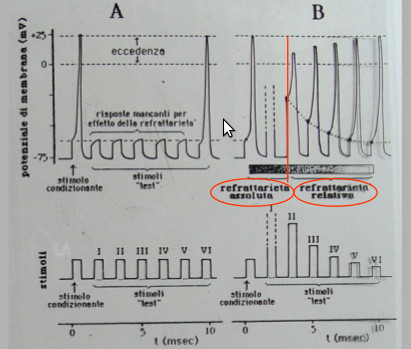
\includegraphics[scale=0.5]{immagine/refrattarieta.jpg}
\caption{B: immediatamente dopo un potenziale di azione, si parla di \emph{refrattarietà assoluta} per cui uno stimolo di qualsiasi intensità è inefficace. Successivamente si parla di \emph{refrattarietà relativa}: lo stimolo test deve essere sufficientemente elevato. In questa fase la soglia, partendo da un valore infinitamente elevato, torna gradualmente al livello di riposo}
\end{figure}

Il periodo refrattario è il tempo in cui la membrana non risponde a stimoli della stessa intensità. si divide in:
\begin{enumerate}
\item{Refrattarietà assoluta: la soglia è all'infinito}
\item{Refrattarietà relativa: si genera un impulso innalzando l'intensità del secondo. La soglia ha un decadimento esponenziale che riflette il fenomeno visto}
\end{enumerate}

La durata della refrattarietà assoluta è correlata alla durata del potenziale di azione, quindi è molto diversa nelle cellule eccitabili di diverso tipo.

\subsection{Fenotipo elettrofisiologico}
Perchè l'impulso è diverso in vari tessuti?

Confrontiamo neurone, fibra muscolare scheletrica e fibra miocardica. Lo stimolo bifasico appena visto per il neurone, non c'è per gli altri due.

Anche la durata è diversa:l'impulso nervoso è il più breve (2 ms), quello muscolare è intermedio (5 ms) e quello cardiaco presenta addirittura un plateau (200 ms). Se dobbiamo stimolare il miocardio infatti dobbiamo deprimere o elevare il plateau!

Ci sono vari farmaci per regolarizzare l'attività cardiaca che entrano in azione in diverse fasi dell'impulso.
Il fenotipo elettrico cambia quindi a seconda dell'uso che ne fa la cellula. 
Per ogni tipo di canali voltaggio-dipendenti, il genoma umano ha un numero di geni multiplo rispetto alla funzione, che codifica per i diversi sottotipi che compaiono nei vari tessuti!

\paragraph{Quanto viaggia un impulso?}

Quanto vuole. Esso percorre tutta la strada della membrana fino alla sinapsi: ad esempio quello generato nel colletto assonico di un motoneurone viaggia \emph{inalterato} fino alla placca motrice. È un apparente paradosso, perchè si dissipa energia e si dovrebbe avere una caduta dell'ampiezza dell'impulso: la membrana produce però il potenziale d'azione attingendo ad una \emph{sua} energia  (potenziali elettrochimici)! Ogni area della membrana quindi ripete il fenomeno dell'impulso \lfreccia grosso dispendio di energia.

I \emph{potenziali di tipo graduato} invece dove vengono generati, gradualmente si estinguono. Devono quindi essere tradotti in potenziali di azioni.

\subsection{Conduzione di un segnale graduato}
Avanzamento di un segnale attraverso la membrana. 

Procediamo in questo modo: utilizziamo una fibra nervosa, generiamo in un certo punto $x_{0}$ un potenziale graduato e poi mettere un elettrodo registrante progressivamente a distanza maggiore dal punto $x_{0}$. Se viene generato in quel punto un segnale di ampiezza $V_{0}$, lo misuriamo nei punti successivi (x1, x2..). Osserviamo un \emph{decadimento esponenziale} del segnale: infatti se generiamo una ddp nel punto $x_{0}$, avendop a riposo -70 mV e dopo il potenziale -60 mV, abbiamo un impulso di 10 mV. Stiamo quindi riducendo la densità di cariche negative all'interno della membrana per un ammontare di 10 mV \lfreccia è come generare una batteria di 10 mV con il polo positivo al lato esterno della membrana e il polo negativo all'interno. La batteria mantiene il suo valore se tra i due poli non passa corrente. 
 
Supponiamo che la mebrana nella regione di $X_{0}$ non abbia resistenza, il segnale procederebbe all'infinito e la batteria non dura! Se invece la resistenza è altissima, il segnale viaggerà pochissimo e la batteria si mantiene.

Quanto lontano posso quindi trovare i 10 mV? Dipende da quanta corrente sfugge lungo la membrana e quanto potrà avanzare lungo la via resistiva dell'assoplasma.

A che distanza il segnale da 10 mV diventerà 1/3? Posso spostarmi molto se la membrana ha alta resistenza (Rm alta) e poco se la membrana perde.

Questo comportamento è definito dalla \emph{costante di spazio}, definita come:
\begin{equation}
\centering
V_{x}=V_{0} e^{\frac{-x}{\lambda}}
\end{equation}

dove $\lambda =\sqrt{\frac{R_{m}}{R_{ass}}}$ è la costante di spazio.\\

Se prendiamo un punto qualsiasi della membrana possiamo quindi valutare quanto un segnale dato in quel punto è risentito nello spazio (costante di spazio) e per quanto tempo (costante di tempo). 

\subsection{Propagazione dell'impulso}
Cos'è che punto per punto scatena l'impulso?

Supponiamo di avere una fibra e produciamo un potenziale di azione in una parte della membrana: cosa dice alla parte successiva della membrana che a sua volta deve produrre un potenziale di azione?

Il potenziale di azione, nella prima fase è una depolarizzazione ampia, che è in grado di sollecitare la parte adiacente in senso depolarizzante. Il potenziale d'azione è quindi risentito come una \emph{corrente depolarizzante} dalla parte adiacente della membrana.

\subsection{Assone gigante}
Come studiamo la permeabilità su questo assone?

Quando inneschiamo un potenziale d'azione, inneschiamo un fenomeno che dipende dal valore del potenziale e dal tempo.

Se vario il potenziale di membrana da un punto ad un altro e lo mentengo a quel valore, qual è la permeabilità della membrana? E se sposto rapidamente il potenziale tra due valori qualsiasi, quanto prontamente la membrana cambia permeabilità?

L'equazione di Goldmann non ci descrive le variazioni di conduttanza, perchè le permeabilità sono costanti: per sapere come varia la permeabilità in funzione del tempo, si è creata una tecnica di registrazione particolare.

\subsection{Current-clamp}
Il metodo consiste nel misurare la differenza di potenziale generata a cavallo della membrana di una cellula (immersa in un mezzo conduttore) dal passaggio di una corrente di intensità nota, ottenuta da un generatore esterno regolabile di \emph{corrente costante}.

Il generatore di corrente ha un feedback interno per cui se la resistenza dell'elettrodo cambia un po' nel tempo, il sistema la compensa \lfreccia \emph{corrente costante} (current clamp).

\begin{figure}[H]
\centering
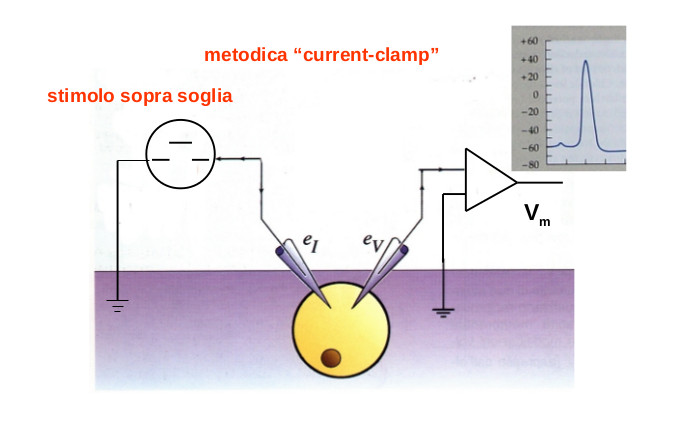
\includegraphics[scale=0.4]{immagine/cc.jpg}
\caption{Rappresentazione schematica del metodo \emph{current clamp}. Il microelettrodo $e_{v}$ permette di misurare le variazioni del potenziale di membrana al passaggio di un impulso di corrente $I_{m}$ iniettato nella cellula tramite l'elettrodo $e_{1}$}
\end{figure}
Usiamo due elettrodi e connettiamo ad uno un \emph{amplificatore operazionale}: esso riceve due ingressi, uno lo chiama + e l'altro -. Ha un morsetto di uscita. In quelli di ingresso entrano due valori di potenziali e in quello di uscita esce una corrente. La corrente è proporzionale al $\Delta V$.

Se registriamo il potenziale di membrana $V_{m}$, registriamo l'impulso.

Ragionando in termini di corrente, notiamo che in corrispondenza dello \emph{step on} di ogni impulso, le variazioni di potenziale non si istaurano istantaneamente, ma raggiungono il loro valore definitivo con \emph{legge esponenziale}.
Questo comportamento equivale a quello di un \emph{circuito RC}: ad una resistenza $R_{m}$ è colegato in parallelo un condensatore $C_{m}$. La corrente erogata dal generatore $I_{g}$ si divide in due componenti:
\begin{itemize}
\item{Componente resistiva $I_{R}$ : percorre la resistenza $R_{m}$ e determina la variazione di potenziale ai suoi capi}
\item{Componente capacitiva $I_{C}$ : va a caricare il condensatore $C_{m}$}
\end{itemize}

Allo step-on dell'impulso, tutte le cariche portate dalla corrente andranno a caricare la capacità $C_{m}$, quindi $I_{C}$ sarà massima e $I_{R}$ nulla. In seguito, mano a mano che il condensatore si carica, la componente capacitiva si riduce e quella resistiva aumenta \lfreccia la differenza di potenziale ai due capi della membrana aumenta.

Quando il condensatore sarà completamente caricato, tutta la corrente passerà attraverso la resistenza e $V_{m}$ raggiungerà un valore finale stazionario.
Questo era in una membrana \emph{ineccitabile}\todo{Sicura? controlla sbobinatura}.

\subsection{Voltage-clamp}
Invece di far passare attravero la membrana correnti di intensità costante e registrare le variazioni del otenziale di membrana (come si fa nel current-clamp), la membrana viene portata a potenziali di clamp prestabiliti, $V_{cl}$, e si registrano le correnti $I_{m}$ necessarie per mantenerla \emph{bloccata} a questi potenziali.

\begin{figure}[H]
\centering
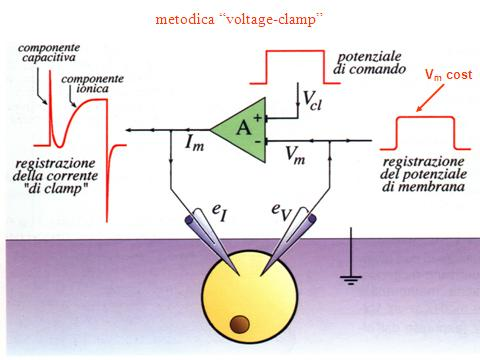
\includegraphics[scale=0.5]{immagine/img1.jpg}
\caption{Sistema Voltage Clamp}
\end{figure}
$V_{cl}$ è erogato da un generatore regolabile in impulsi, di volta in volta predisposto al valore al quale si desidera bloccare il potenziale di membrana.

Se i due potenziali dell'amplificatore, $V_{m}$ e $V_{cl}$, sono uguali, la corrente sarà pari a 0.

Se $V_{m}$ cambia (e $V_{cl}$ costante), a seconda di dove cambia, se è in senso depolarizzante fluirà corrente iperpolarizzante, se è in senso iperpolarizzante la corrente sarà depolarizzante \lfreccia ecco perchè è un sistema a feedback : il sistema riposta sempre il valore di $V_{m}$ verso quello di $V_{cl}$.

Se $V_{cl}$ cambia, fluirà una corrente che tende a spostare $V_{m}$ a quel valore e continuerà a fluire fino a che quel valore deve essere mantenuto. 

\paragraph{Esempio}
Supponiamo di avere $V_{m}$ = -70 mV e $V_{cl}$ = -60 mV. Uscirà una corrente che porta la membrana a -60 mV: questa corrente deve fluire per tutto il tempo durante il quale voglio mantenere questo potenziale di -60 mV. Chiamiamo questa corrente \emph{corrente di correzione}.

Facciamo quindi diventare il potenziale di comando, che ho scelto io, il potenziale di membrana.

Se iperpolarizzo, avrò una corrente attraverso il condensatore che si estingue esponenzialmente: mi rimane il valore di corrente che mantiene $V_{cl}$.

Se depolarizzo, succede il contrario.

Se voglio mantenere un voltaggio maggiore, mi serve una corrente maggiore. Giustifico il tutto con un circuito RC. Il potenziale di comando viene quindi variato istantaneamente e mantenuto nel tempo.

Se ho una \emph{membrana eccitabile}, se $V_{cl}$  è superiore alla soglia, vedo sia la \emph{corrente capacitiva} che quella data dalla \emph{componente ionica}, cosa che non vedo sotto soglia o in senso iperpolarizzante perchè in questo caso fluiscono gli ioni! Vedo quindi la corrente che entra nella membrana e quella che esce, ed entrambe sono correnti attive. Il picco in basso (caduta della corrente dopo la componente ionica) è dovuto alla scarica del condensatore.

Il vantaggio del metodo \emph{voltage clamp} è che possiamo \emph{misurare la componente ionica della corrente transmembranaria separatamente dalla componente capacitiva}. Anche le correnti di clamp infatti sono formate da due tipi di corrente:
\begin{itemize}
\item{Corrente capacitiva $I_{C}$}
\item{Corrente ionica $I_{i}$}
\end{itemize}

Nel momento in cui viene imposto il potenziale di comando $V_{cl}$, la capacità $C_{m}$ viene caricata in modo \emph{istantaneo} \lfreccia la corrente capacitiva è molto intensa ma di breve durata, quindi va estinguendosi velocemente.

Il decorso temporale della corrente ionica quindi potrà essere analizzato correttamente perchè cronologicamente separato da quello della corrente capacitiva.
La corrente capacitiva ha la possibilità di andare a 0 esponenzialmente.

La corrente passiva si forma attraverso i canali passivi.

La corrente ionica è data da ioni che la membrana fa passare perchè i canali voltaggio-sensibili sono stati aperti dal raggiungimento della soglia.

Noi stiamo quindi spostando il valore di $V_{m}$ e vedendo quali sono le correnti che entrano in gioco. Durante il otenziale di comando, non cambia il valore ma cambia il tempo: descriviamo quindi le conduttanze in funzione del tempo a voltaggio costante. Possiamo descrivere questo fenomeno semplicemente misurando le correnti.

(3.10.2014)
 \todo{finisci lezione}.
  
\paragraph{Esperimento}

La membrana come l’abbiamo descritta è sede di un suo potenziale che chiamiamo Rest. A riposo, esso è dato non da un potenziale di equilibrio ma da uno di \emph{diffusione}, quindi nella nostra situazione abbiamo un valore di -70 mV che significa che stanno fluendo almeno due correnti: \emph{sta entrando sodio ed uscendo potassio}.

Entra sodio perché il potenziale di membrana è -70 mV e il potenziale del sodio, è -45 mV: essi sono diversi e così il sodio è spinto ad entrare; esce invece il potassio perché il  potenziale -70 mV, è più depolarizzato rispetto al suo potenziale di equilibrio e il potassio esce. 

Questo flusso continuo viene compensato dalla \emph{pompa sodio potassio}. Se vogliamo spostare il valore del potenziale di membrana, che in condizione stazionaria rimarrebbe a -70 mV, per la legge di Goldmann dobbiamo muovere la corrente attraverso la membrana: è infatti l’unico modo per cambiare la densità di carica ai due lati di essa. Ecco perché quando sia in senso depolarizzante che in senso iperpolarizzante (potassio iperpolarizzante) la corrente fluisce, per tutto il tempo che mantengo a -90 mV, fluisce all’interno. 

Facendo l’opposto: se vado a -50 mV avrò corrente che inverte di direzione ma fluirà fino a quando mantengo il potenziale di membrana a -50 mV. 

\paragraph{Esperimento}

Facciamo variare nel tempo il potenziale di comando, per fare questo ricorriamo al secondo programma. Tutto è come prima tranne che il potenziale di comando (in questo caso faremo l’esempio di una depolarizzazione) cambierà di 10 millivolt in senso depolarizzante, da -70 mV andremo a -60 mV e registreremo la corrente come prima. 
Vedremo che il potenziale di comando andrà da una variazione di 0 a una di 10 mV in senso depolarizzante. Dunque da -70 mV andremo a -60 mV per ritornare a -70 mV, tutto ciò per un certo numero di volte. Quindi nello schermo a destra vediamo come varia il potenziale di comando e a sinistra come si comporta la corrente in funzione del tempo. 
A destra il potenziale si sposta in alto e in basso alternativamente. Quando è in alto avremo -60 e quando in basso -70. A sinistra la corrente varierà da 0 ad 1 nanoAmpère per tutto il tempo in cui viene mantenuto il potenziale di comando a -60.
Ingrandiamo i transitori ( grafici gialli su sfondo nero). In quello di sinistra vediamo la corrente che fa una transizione da zero a 1 depolarizzante, il voltaggio a destra, è istantaneamente cambiato. La corrente va incontro ad una carica istantanea del condensatore, una caduta esponenziale e poi si setta ad un valore che misuriamo che è 1 nA (A = ampère).

\paragraph{}
Se la membrana è ineccitabile o se in una membrana eccitabile non facciamo tendere ad aprirsi maggiormente i canali voltaggio dipendenti, vediamo che la prima fase del fenomeno è caratterizzata dalla corrente di capacità o capacitiva (la corrente capacitiva è quella che va a caricare il condensatore ovvero fa accumulare cariche su una faccia della matrice lipidica) e per sua proprietà subito dopo lo va a scaricare. Ad cui si somma una seconda corrente che è la resistiva ed è rettangolare (corrente resistiva è la corrente che percorre la resistenza ovvero i canali ionici). 

\subsubsection{Forma delle correnti}
\begin{figure}[H]
\centering
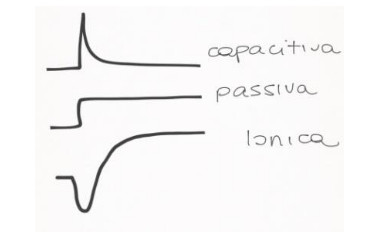
\includegraphics[scale=0.5]{immagine/correnti.jpg}
\caption{Schema delle correnti in \emph{voltage clamp}}
\end{figure}

La \emph{corrente capacitiva} ha il picco; allo stato stazionario,la corrente è chiamata è chiamata \emph{di perdita o passiva} ed è rettangolare.
La prima corrente non attraversa la membrana ma carica o scarica i piatti del condensatore; la seconda passerà, in una membrana ineccitabile, attraverso i \emph{canali passivi}. 

La fase rapida esponenziale della corrente capacitiva, poi con decadimento altrettanto veloce, serve quindi a caricare i piatti del condensatore prima di far fluire la corrente di perdita attraverso i canali passivi. Se non abbiamo stimolato i canali voltaggio dipendenti la resistenza non cambia.

Una volta caricato il condensatore, la corrente fluisce attraverso la resistenza (i canali passivi in questo caso). Tutto ciò se parliamo di cellule ineccitabili o di cellule eccitabili nelle quali non attiviamo i canali voltaggio dipendenti, che restano inattivi perché siamo sotto soglia. 

Supponiamo invece di depolarizzare sopra soglia una \emph{membrana eccitabile}: quando portiamo il potenziale sopra la soglia, si apriranno i canali voltaggio dipendenti.

Se avessimo un circuito aperto, ovvero senza la possibilità di operare manipolazioni da parte del potenziale di comando, registreremo il potenziale d’azione, ma la membrana non può produrlo perché quando la membrana tende a depolarizzare, il sistema di clamp la blocca. I flussi di corrente, generati dai canali ionici voltaggio dipendenti, vanno corretti: ecco per quale motivo andiamo a registrare, oltre alla corrente di capacità e alla corrente di perdita passiva, una corrente entrante ed una uscente. Queste due, per il fatto stesso che si manifestano solo in membrane eccitabili al di sopra di soglia, sono le \emph{correnti attive} che attraversano i canali voltaggio dipendenti responsabili dell’eccitabilità elettrica.

\paragraph{Correnti entranti ed uscenti}

Le correnti si definiscono \emph{entranti} o \emph{uscenti}, non in relazione ai due elettrodi, ma in relazione alla membrana. 

Una \emph{corrente uscente} è una corrente che \emph{depolarizza} perché le cariche positive andranno a neutralizzare parzialmente le cariche negative interne della membrana. 

Per la ragione opposta, una \emph{corrente entrante} nella membrana sarà \emph{iperpolarizzante} perché le cariche positive usciranno dalla cellula.

\begin{figure}[H]
\centering
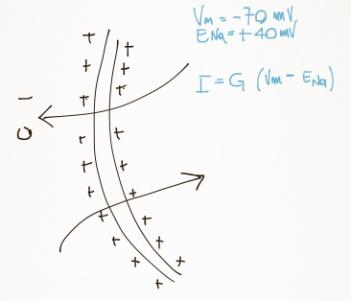
\includegraphics[scale=0.5]{immagine/cerr.jpg}
\end{figure}

Supponiamo quindi ora di aprire canali per il sodio, esso dovrebbe entrare perché il potenziale di membrana è in genere negativo e il potenziale di equilibrio del sodio è +40/45, lontanissimo (in figura vediamo il calcolo).

La differenza tra $V_{m}$ ed $E_{a}$ è molto grande pechè $V_{m}$ è molto negativa ed $E_{a}$ è molto positiva. Inoltre il sodio entra perchè carico positivamente, quindi viene attratto all’interno; è più concentrato all'esterno \lfreccia sia la forza elettrica che la forza chimica fanno entrare il sodio.

Se cambiassimo la concentrazione del sodio, ovvero mettendo più sodio all'interno della cellula, vedremmo, all'apertura dei canali, uscire il sodio. Potrei progettare una concentrazione interna tale per cui se apro i canali, il sodio esce fuori, per esempio levando sodio extracellulare e mettendo 300-400 mmoli all’interno.

\paragraph{Come si ottiene la forma delle correnti?}

Supponiamo di avere la membrana nella sua situazione stazionaria: negativa all’interno, flusso di sodio verso l’interno verso l’interno e uscita di potassio (modeste!!!), valore di potenziale -70 mV stazionario.

Se vogliamo cambiare il potenziale di membrana dobbiamo distribuire diversamente le cariche, ciò significa che dovrò ad esempio avere un eccesso di carica negativa all’interno rispetto alla faccia esterna. 

Se il sistema non è eccitabile, le permeabilità sono costanti e così basterà generare una corrente capacitiva ed una passiva, ovvero resistiva, per variare il valore del potenziale. Se nel fare questo mi variano altre permeabilità io dovrò far fronte anche anche a quelle, facendo fluire delle correnti in aggiunta in altre direzioni: entranti ed uscenti. 

Quando si genera un \emph{potenziale d’azione}, c’è una massiccia entrata di sodio, molto maggiore di quella che normalmente avviene allo stato stazionario, seguita da un’uscita di potassio. Per contrastare queste e mantenere costante il potenziale, siccome il potenziale è soprasoglia, il sistema che è chiuso, non fa realizzare il potenziale di azione come variazione di voltaggio ma le correnti ioniche del potenziale d’azione fluiscono e io le ho tamponate col sistema del voltage clamp. 
Dunque il potenziale d’azione si realizza sotto forma di flussi ionici ma io li “tampono” facendo fluire corrente.

\subsubsection{Come misuro il flusso ionico?}
Il voltaggio o differenza di potenziale è una condizione potenziale come lo è la pressione in un sistema idraulico.

Pressione sta a voltaggio e flusso di un fluido sta a corrente. 

Prendiamo un pallone e lo insuffliamo con un flusso di aria costante. Questo pallone ha alcuni forellini e sempre quelli, in cui l'aria potrà uscire parzialmente. Altra aria tenderà ad entrare cercando di mantenere la pressione costante del pallone. Questa situazione è simile allo \emph{stato stazionario della membrana}: abbiamo continuamente ingresso di aria, nel nostro caso è dato delle \emph{pompe}, e poi abbiamo delle fughe passive che mantengono il potenziale ad un certo valore. Se voglio cambiare questo valore devo insufflare altra aria, che oltre a mantenere il valore di P mi deve portare ad un valore maggiore per contrastare l’effetto di uscita. Perché devo continuare a far fluire? perchè se no le perdite tenderanno a far andare la pressione ad un valore non desiderato dal potenziale di comando.
Data una resistenza, una perdita, devo dare un surplus per mantenere costante la pressione ad un valore maggiore.
Supponiamo che si abbia ora un così detto diavoletto che, quando legge la pressione più alta, apre un foro. Per mantenere P costante, a livello alto, dovrei dare ancora più pressione, è quello che accade in questa situazione se il flusso d’aria viene sostituito dal flusso di corrente. 

\emph{Una volta che il potenziale di membrana ha raggiunto il valore del potenziale di comando, la corrente smette di fluire?}
 
Il sistema di controllo deve avere la caratteristica dell’\emph{estrema velocità}: come il potenziale di membrana tende a variare, la corrente immediatamente spenge la variazione. 
Il profilo del potenziale di comando lo troviamo ripetuto al livello del voltaggio di membrana, in altri termini, il potenziale di membrana, come si sposta di poco, viene riportato al valore desiderato. 
In basso nel grafico, avevamo solo i canali passivi aperti, in alto nel grafico si aprono anche i canali attivi, che fanno passare il potassio. Quando questi ultimi si aprono, io dovrò dare un’extracorrente per neutralizzare il fenomeno. 
\todo{manca quel pezzo incomprensibile}

\subsubsection{Attribuire identità ionica alle varie correnti}

Per capire quale ione è responsabile di quale corrente ionica posso fare esperimenti in cui cambio la concentrazione di uno ione alla volta all'interno o all'esterno della membrana.
 
\begin{figure}[H]
\centering
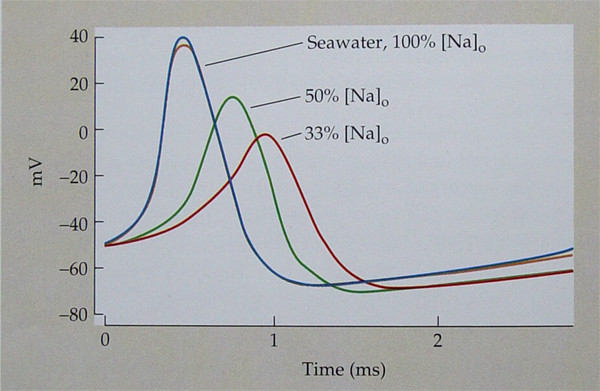
\includegraphics[scale=0.4]{immagine/cor.jpg}
\end{figure}

Supponiamo di metter meno sodio o niente sodio all'esterno: vediamo il fenomeno in figura. Abbiamo l’assone di calamaro, un potenziale d’azione normale in acqua artificiale (ricordo che l’ambiente interno di questi animali marini è conforme all’acqua di mare) \lfreccia con 100 \% di sodio ho un certo potenziale, se lo porto al 50 \% avrò un potenziale di azione  ritardato ed attenuato, se porto il sodio al 33 \% ancora di più, se metto zero sodio all'esterno il potenziale d'azione scompare. 

\emph{Come faccio dunque ad attribuire alle correnti il ruolo dei vari ioni?}

Ricordando la formula che descrive la corrente in funzione della conduttanza e delle forza elettromotrice, $I_{i} = G_{i}  (V_{m} - E_{i})$, \emph{la FEM è data dal potenziale di membrana che misuro e dal potenziale di equilibrio}. Quest’ultimo dipende dall’\emph{equazione di Nernst} e dal salto di concentrazione interna ed esterna dello ione preso in esame. Se vario le concentrazioni, allora deve variare la corrente.

Andiamo a vedere allora cosa succede se registro le correnti ioniche isolate dalla componente capacitiva di linkage, che sono correnti verso l’interno e verso l’esterno. 
Sostituisco il sodio cloruro col cloruro di colina, esso non passa come il sodio attraverso il canali del sodio, così l'influsso del sodio non può manifestarsi, anzi paradossalmente ho un rovesciamento della corrente precoce: il sodio anziché entrare, esce, perché aprendosi i canali, il sodio è tutto dentro. La situazione non è un’alterazione del sistema perché se ritorno alla concentrazione iniziale di sodio il sistema torna alla normalità.

Siccome se faccio la stessa operazione col \emph{potassio} il fenomeno non accade, siamo autorizzati a dire che \emph{la corrente precoce, siccome segue il potenziale elettrochimico del sodio e richiede che all’esterno ci sia il sodio, è portata dagli ioni sodio}.

Per confermare questo posso lasciare $E_{i}$ stazionaria come è naturalmente, quindi con il sodio extracellulare nelle solite condizioni, e modificare il potenziale di comando. Se vado a modificarlo dovrei avere secondo l’equazione che, se porto il potenziale di comando al valore del potenziale di equilibrio del sodio, dovrò dare corrente 0 (Vm=Ea) qualsiasi sia G perché non ho più forza premente:

\begin{figure}[H]
\centering
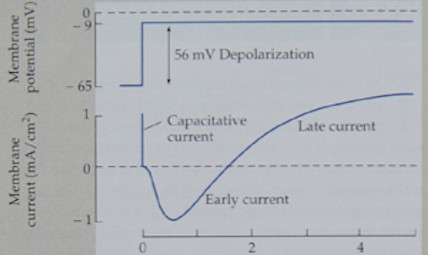
\includegraphics[scale=0.5]{immagine/potassio.jpg}
\end{figure}

Ho diversi potenziali di comando in slide. Se vado a +52, che è il potenziale di equilibrio del calamaro gigante, scompare la corrente entrante:

\begin{figure}[H]
\centering
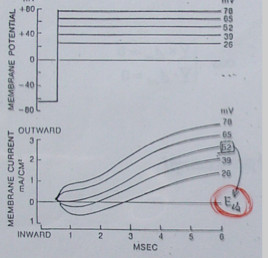
\includegraphics[scale=0.5]{immagine/52.jpg}
\end{figure}
 
Questo ci dice esplicitamente che la forza premente è esattamente corrispondente a quanto si discosta il potenziale di membrana dal potenziale di equilibrio del sodio.
Se sposto Vm oltre il potenziale di equilibrio il segno della differenza cambia e cambia il segno della corrente.


(9.12.2014)

\subsubsection{Qual è il significato delle correnti ioniche legate al voltage clamp?}

Suddividiamo le correnti capacitive e di perdita in passive ed attive (le passive sono le B della slide dei voltage clamp con tutti i grafici, le attive sono la C e la D)\todo{allega slide: senti mares}.

\paragraph{Correnti passive}

Se in una cellula non eccitabile inseriamo potenziali iperpolarizzanti o depolarizzanti otterremo correnti che servono a portare ad un dato voltaggio una membrana che ha una certa resistenza. Sono le correnti che il sistema biofisico associa all'assone gigante. Queste correnti fluiscono attraverso canali passivi, la cui probabilità di apertura non cambia al variare di parametri esterni. Nella cellula eccitabile abbiamo anche una corrente bifasica aggiuntiva: sono \emph{correnti attive}.

\paragraph{Correnti attive}
Una corrente di ioni Cl verso l'esterno depolarizza la membrana \lfreccia genera nei canali attivi voltaggio dipendente una corrente \emph{bifasica}. Quali sono gli ioni e i canali coinvolti?

Abbiamo una corrente \emph{precoce} ed una \emph{tardiva}: la precoce è entrante, la tardiva  è uscente. PEr identificare gli ioni coinvolti, sapendo che una corrente è prodotta da una condurttanza (permeabilità) moltiplicata per una ddp (voltaggio di comando), troviamo il potenziale di equilibrio dell ione, che dipende dall'equazione di Nerst. Variando le concentrazioni ioniche, possiamo vedere se una corrente risente di questa variazione. Si sapeva già che esistevano permeabilità selettive per Na e K.

\subsubsection{Quali ioni sono coinvolti?}
Se si taglia il Na extracellulare, il picco dei mV ritarda e diventa più attenuato. 
\paragraph{Esperimento}
Se sottraiamo le stimolazioni speculari generate dalle correnti e sostituiamo il Na extracellulare con il cloruro di colina, la corrente precoce si rovescia di polarità (Il sistema è reversibile). Perturbando quindi il otenziale di equilibrio del Na, la corrente precoce ne risente: deve quindi consistere in un passaggio di sodio. L'inversione della polarità è data dal fatto che la differenza $V_{m} - E_{i}$ si inverte di segno.
\paragraph{Esperimento}
Possiamo altenrativamente giovare sul potenziale di comando $V_{m}$: se esso raggiunge il potenziale di equilibrio $E_{i}$, la corrente si annulla. Se mettiamo il potenziale di comando a vari valori, attorno a +52 osserviame che: sotto, vediamo ancora una corrente entrante ed una uscente; a +52 non vediamo più la corrente precoce; sopra +52 vediamo una corrente precoce invertita di direzione.

La corrente precoce consiste quindi in un ingresso di Na attraverso canali voltaggio di dipendente.

\paragraph{Esprerimento}
Diamo potenziali di comando progressivamente più ampi: vediamo una famiglia di curve. Se depolarizziamo poco (primo gradino), osserviamo una curva con una piccola e lenta corrente entrante ed una quasi nulla corrente uscente. Se aumentiamo, la corrente entrante diventa sempre più ampia, fino a ridursi di ampiezza e rovesciarsi.

Man a mano che depolarizzo, aumento la probagilità di apertura dei canali di Na (G); se aumento ancora, mi avvicino al potenziale di equilibrio, quindi aumento si la permeabilità ma diminuisce la forza motrice.

\subsubsection{Quali sono i canali coinvolti?}

\paragraph{Tossine di veleni}

Con l'uso di tossine di veleni, sostanze che alcune specie esprimono ed applicano per difesa. Queste sostanze sono altamente specifiche, e colpiscono selettivamente determinate molecole funzionali. Una tossina applicata ad un sistema vivente riesce anche a bloccare i movimenti, l'eccitabilità e la trasmissione sinaptica.

Ad esmepio la \emph{tetrodotossina} si lega al canale voltaggio dipendente e lo blocca: dopo aver fatto registrazioni di controllo, somministrando la tossina rimangono solo le correnti uscenti ripulite completamente dalle correnti entranti.

Il \emph{tetrotilammonio} invece fa sparire completamente le correnti uscenti.

Se sostituiamo gran parte del potassio intracellulare ad esempio con del cesio, presentiamo una forza elettromotrice pari a 0 per K (o Na) e si annullano le correnti tardive.

\paragraph{}
Le correnti entranti ed uscenti, sulla stessa scala temporale, appaiono sfasate; inoltre le correnti tardive permangono nonostante venga mantenuto il potenziale di comando depolarizzato, le precoci invece scompaiono.

Il fatto che i canali Na non vengono mantenuti aperti per tutto il tempo del potenziale di comando è detto \emph{fenomeno di intattivazione}. Chiamiamo \emph{fase di attivazione} l'aumento della probabilità di apertura di una classe di canali; \emph{fase di deattivazione} il decadimento esponenziale di una corrente. Questo per la corrente K.

Per la corrente Na, la corrente va ad un picco e poi anzichè mantenenrsi come la corrente K, ritorna a 0. Abbiamo quindi la fase di \emph{inattivazione}, diversa dalla deattvazione che è una riduzione della permmeabilità al valore iniziale dovuta al fatto che cessa lo stimolo. L'inattivazione è una riduzione di permeabilità che avviene \emph{durante} la persistenza dello stimolo.

L'inattivazione ci suggerisce che il canale per Na deve avere delle proprietà diverse, aggiuntive rispetto al canale K: mentre attivaizone e deattivazione le goiustifichiamo immaginando che il canale abbia dei gruppi funzionali che fanno da dipoli (separazione di cariche) che al cambiare del potenziale di membrana possono orientarsi diversamente causando la variaizone di permeabilità (fa da \emph{cancello}). L'inattivazione invece non si giustifica con l'esistenza di un semplice \emph{cancello}: dobbiamo aggiungere un secondo meccanismo, preannunciato da un esperimento.

\paragraph{Esperimento di perfusione con pronasi \todo{chiedi a ricevimento}}
Chiarisce che le porzioni di canali responsabili di attivazione/deattivazione e inattivazione, vediamo che sono 2 porzioni diverse.

\begin{figure}[H]
\centering
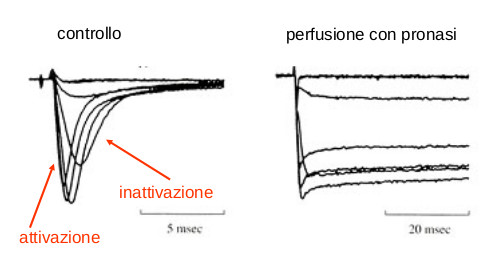
\includegraphics[scale=0.4]{immagine/pronasi.jpg}
\caption{Perfusione con pronasi}
\end{figure}
Quindi attaccando con un enzima proteolitico (pronasi) il canale, una parte del canale attaccata mi rimuove il fenomeno di inattivazione, ma non quello di attivazione-deattivazione, l'altra fa il contrario.
L'inattivaizone è una risposta voltaggio dipendente.

\paragraph{Esperimento}
Stimolo test che dà una corrente entrante-uscente. Lo ripeto altre volte, ma prima di fare lo stimolo test che arriva allo stesso livello di depolarizzazione, iperpolarizzo o depolarizzo a diversi valori (stimolo condizionante). 

\begin{figure}[H]
\centering
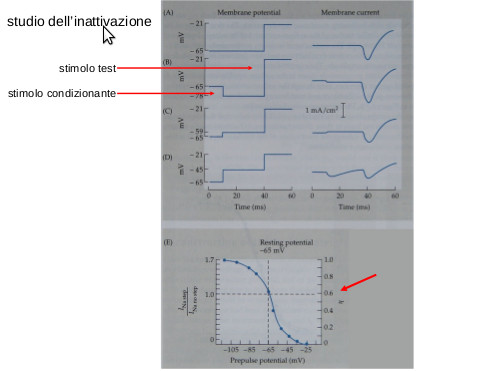
\includegraphics[scale=0.6]{immagine/inatt.jpg}
\end{figure}

Se iperpolarizzo prima dello stimolo test, la corrente Na aumenta fino ad un massimo (-110 mV) (rapporto 1,7).

Se depolarizzo prima dello stimolo test, la corrente Na si riduce fino ad azzerarsi (-25 mV) (rapporto 0).

Dividendo le due correnti ottenute a diversi valori di prepotenziale, per quella generata dal solo stimolo test  (normalizzazione): se queste correnti saranno più grandi, avremo un numero maggiore di 1 e viceversa.
Otteniamo la \emph{curva di inattivazione} mettendo sulle ascisse nel mezzo -65 mV (potenziale di membrana), a destra la iperpolarizzazione e a sinistra l'iperpolarizzazione.

Al valore di rapporto uguale a 1, se lo metto come valore massimo che posso ottenere e 0 come minimo, vedo che la modulazione dovuta all'inattivazione varia variando il potenziale,  ma mi dice che il fenomeno è già presente al potenziale di riposo di -65 mV: se non ci fosse inattivaiozne, dovrei vedere il valore massimo della corrente.

L'inattivazione possiamo immaginarla come una buca di potenziale. Al potenziale di membrana a riposo, abbiamo già una frazione di canali che è inattivata: se preiperpolarizziamo, riportiamo questi canali nella condizione di chiuso-apribile o aperti.

\subsubsection{Canale ionico Na}
Nel canale ionico di Na abbiamo due cancelli, uno di \emph{inattivazione} e uno di \emph{attivazione-deattivazione}.

Il primo è lento, il secondo è più veloce: ecco perchè l'inattivazione avviene dopo un certo tempo che noi abbiamo variato il potenziale di membrana.

Con la depolarizzazione si apre il cancello veloce, entra Na e la porta di inattivazione comincia a spostarsi, e dopo un pochino chiude la bocca del canale: la corrente è quindi compromessa anche se il cancello veloce è aperto. La curva di inattivazione può essere interpretata in questo modo! L'inattivazione è rappresentata come un minimo accentuato perchè, per riportare alla condizione attiva, dobbiamo portare il potenziale di membrana almeno alla soglia di riposo. Se diamo pronasi, compromettiamo il meccanismo di intattivazione.

\paragraph{Esperimento}
Poichè conosciamo esattamente la sequenza dei canali, attraverso \emph{mutagenesi sito-diretta} produciamo canali ionici alterati che presentano la parte che chiude il cancello lento alterata o assente. Se aumentiamo o riduciamo quella parte (è tipo un picciolo), abbiamo una cinetica diversa; se invece proprio la eliminiamo abbiamo lo stesso risutato che con la pronasi. Se somministriamo un peptide simile al picciolo, ritroviamo fenomeno di intattivazione.

\subsection{Come varia la permeabilità nel tempo in funzione del voltaggio}
Possiamo ricavare la variazione di permeabilità in questo modo:
\begin{equation}
\centering
I_{i}(t)=G_{i}(t) (V_{m}-E{i})
\end{equation}

Possiamo quindi ricavare la conduttanza G. Il segno algebrico di G discrimina l'inversione del potenziale man a mano che depolarizziamo. 

\begin{figure}[H]
\centering
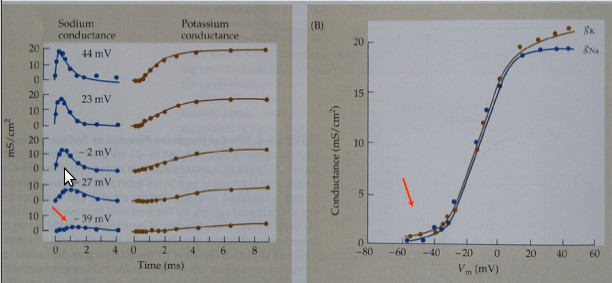
\includegraphics[scale=0.5]{immagine/conduttanze.jpg}
\caption{Grafico della conduttanza in funzione di $V_{m}$ per $K^{+}$ ed $Na^{+}$}
\end{figure}
Se mettiamo i picchi delle conduttanze in funzione del voltaggio, vediamo che le curve per K ed Na sono molto simili: i canali infatti hanno la porzione che risente del voltaggio molto simile tra loro. Non ci stupisce quindi che la dipendenza dal voltaggio sia simile. Notiamo però che le conduttanze per il K a bassi potenziali sono molto lente, mentre quelle di Na sono più precoci.

Se depolarizziamo la membrana, $G_{Na}$ aumenta: aumenta quindi la corrente sodio, che è entrante \lfreccia aumenta la depolarizzaizone (feedback positivo) che opera per produrre variazioni esplosive.

A livello del K, $G_{K}$ produce una corrente uscente che tende a spegnere la depolarizzazione (iperpolarizza \lfreccia feedback negativo).

Una volta fatta una serie di misure, portando il potenziale di membrana da un valore di partenza ad un altro, possiamo studiare l'entità delle correnti e come esse variano. Sapendo che corrente produco in funzione del tempo passando da un potenziale ad un altro, posso convertire la corrente in funizone del tempo in conduttanza, conoscendo la resistenza della membrana. Queste variazioni reciproche vengono conglobate e il modello ci produce un tracciato (V) che è la variazione di potenziale prevista dal modello (è il potenziale di azione dell'assone gigante di calamaro). A destra abbiamo la conduttanza di Na (azzurra) e di K (ritardata). 
Quando viene prodotto un impulso nervoso, si ha aumento transitorio di permeabilità di Na e K (attivazione) a cui segue una riduzione di permeabilità per il Na, poichè il potenziale di membrana non riesce a raggiungere il potenziale di equilibrio del Na, si ferma prima perchè la conduttanza nei pressi del picco si inverte. La conduttanza al K è molto più tardiva e ha un picco nella fase discendente del potenziale di aizone. A questo punto domina solo la conduttanza del potassio: ecco perchè il potenziale di membrana non torna al suo valore ma si avvicina a quello di equilibrio del potassio.

Le due fasi depolarizzanti e ripolarizzanti del potenziale di azione vengono generate dal fatto che \emph{le due conduttanze di Na e K sono sfasate}: se fossero contemporanee, non avremmo la possiblità di generare un impulso.

Possiamo così spiegare diversi parametri descritti dal potenziale di azione.

\subsubsection{Soglia}
La probabilità di apertura di un canale inizia ad aumentare quando raggiungo il valore di potenziale soglia. Questo concetto di valore soglia non è da associare ad un canale ma alla membrana: il valore soglia corrisponde al valore del potenziale di membrana a cui la variazione di $G_{Na}$ si manifesta in modo rilevante e precoce rispetto a $G_{K}$ (quando è appena superiore).

\subsubsection{Periodi refrattari}
Il periodo refrattario \emph{assoluto} si spiega con l'inattivazione del canale Na. Per quanto depolarizziamo, li troviamo inattivati.

Il periodo refrattario \emph{relativo} è più tardivo ed ha a che fare con il valore di $G_{K}$. Essa produce un freno all'eccitazione. La conduttanza del potassio, quando quella del Na torna a livello normale, predomina ed ostacola la membrana in senso depolarizzante.

\subsubsection{Eccedenza positiva}
La membrana dominata da conduttanza del Na (canali Na aperti), tende a raggiungere il potenziale di equilibrio del Na: l'interno diventa positivo (ciò non accade a causa dell'inattivazione).

\subsubsection{Eccedenza negativa}
Perchè in un certo momento è presente solo la conduttanza del K.

\subsubsection{Sfasamento conduttanze}
Serve a poter generare l'impulso.

\subsection{Come si propaga il potenziale di azione}
L'ingresso di Na tende a depolarizzare e la corrente di Na (attiva) esce attraverso i canali passivi. Ciò determina attivazione dei canali di Na voltaggio dipendenti della regione contigua della membrana. all'ingresso di Na serve l'uscita attiva di K nella regione che ha appena ospitato l'entrata di Na \lfreccia quella regione diventa refrattaria: la conduttanza al potassio spegne l'eccitazione. Ciò non significa che il potenziale di azione vada in una sola direzione: è importante con che polarità si genera il potenziale. 

In una fibra amielinica, la velocità di conduizone dipende dal diametro. Nella fibra mielinica, se andiamo a vedere con degli anticorpi che riconoscono i canali Na (verdi) e K (rossi) voltaggio dipendenti, quelli Na hanno alta densità nella regione nodale, mentre K si collocano nella regione adiacente. Anzichè andare per regioni contigue, l'attivazione dei canali di Na avviene tra un nodo e l'altro.

(10.12.2014)
\section{Trasduzione del segnale}
Presuppone un canale di comunicazione (giunzione Gap ecc).

Un segnale elettrico condotto lungo la membrana dell'elemento presinaptico potrebbe fluire nell'elemento postsinaptico. Una corrente depolarizzante, uscente attraverso canali passivi, può fluire attraverso il canale di comunicazione ed uscire dalla membrana del secondo elemento \lfreccia depolarizzazione anche nell'elemento post sinaptico. (\textbf{Sinapsi elettrica})

In una \textbf{sinapsi chimica} (vallo) non c'è collegamento diretto tra i due elementi, e la ripartizione della corrente è nettamente a vantaggio della via che resta nel liquido extracellulare: la membrana dell'elemento post sinaptico infatti ha una resistenza molto alta. Per passarvi, il segnale elettrico deve essere convertito tramite un processo chimico in segnale chimico.

Se registriamo in due cellule accoppiate con giunzioni GAP con 3 elettrodi, due nell'elemento A ed uno nell'elemento B, e applichiamo una corrente. Nell'elemento A si ha una variazione di potenziale maggiore rispetto a quella che troviamo in B, poichè la giunzione GAP la attenua.

\subsection{Sinapsi elettriche}
Caratterizzate da \emph{giunzioni GAP}. Questi accoppiamenti elettrici sono resi possibili dalle \emph{connessine}, costituite da 6 subunità che si dispongono in varie conformazioni: quella aperta (\emph{connessone})lascia un varco di 2 nm (quello di un canale ionico è 0,6 nm!), molto grande rispetto al canale ionico. Se quindi il canale ionico permetteva una certa selettività, nel caso delle connessine ciò non avviene: tutte le specie ioniche possono attraversare il connessone, ma anche nucleotidi \lfreccia comunicazione elettrica e metabolica \footnote{Molti dei nostri epiteli sono tappezzate da cellule a palizzata contigue, molte delle quali sono in comunicazione (metabolica ed elettrica) tra loro.}.

Cellule connesse da giunzioni GAP sono \emph{accoppiate elettricamente e metabolicamente}.

L'apertura o meno dei connessoni dipende da pH e $Ca^{2+}$: se il pH si riduce o il $Ca^{2+}$ si eleva, si ha la chiusura della comunicazione, perchè sono segni di cellule danneggiate. 

Possiamo studiare questi fenomeni con le tecniche \emph{fluorescenti}, ad esempio indicatori per gli ioni di interesse. Ci sono molecole chelanti il $Ca^{2+}$, come Fluo-3: sono \emph{tamponi} per il $Ca^{2+}$, e vengono usati per garantire una concentrazione di $Ca^{2+}$ libero controllata. Quando la molecola lega $Ca^{2+}$ e viene irraggiata a 480 nm, emette a 520 nm (se non lega $Ca^{2+}$, non emette). Per far legare il $Ca^{2+}$, delle esterasi liberano le chele della molecola di Fluo-3 e le permettono di legarlo.

A 4 \textcelsius iniziano a non funzionare più le sinapsi chimiche.

\subsection{Sinapsi chimiche}
Le troviamo nel sistema neuromuscolare e nel sistema nervoso centrale (neuro-neuronali). Questi circuiti di fuga devono garantire una \emph{fedeltà di trasmissione} dalla cellula presinaptica a quella postsinaptica.

Sono stati istituiti due modelli sperimentali: \emph{sinapsi gigante} e \emph{placca motrice}.

\paragraph{Sinapsi gigante}
Possiamo inserire 3-4 elettrodi, due nel pre e due nel post sinaptico, in vicinanza della regione in cui avvengono i fenomeni. Il neurotrasmettitore è il \emph{glutammato}. 

Se mettiamo una coppia di elettrodi stimolanti nell'elemento pesinaptico, insieme ad una pipetta, ed un elettrodo nel post, possiamo registrare nella cellula post sinaptica, con un certo ritardo, una variazione di potenziale graduata, rispetto all'arrivo dello stimolo del pre sinaptico. Il ritardo, nell'uomo, va da 1 a pochi mm.

Se aggiungiamo \emph{tetrorodossina} (TTX), che blocca i canali voltaggio dipendenti, a bassissima concentrazione, in modo da avvelenare lentamente il sistema, l'attivazione del potenziale post-snaptico avviene progressivamente. Il potenziale graduato si riduce perche TTX, agendo lentamente, riduce sempre di più sul lato presinaptico il numero di canali Na ancora non bloccati. 
\begin{figure}[H]
\centering
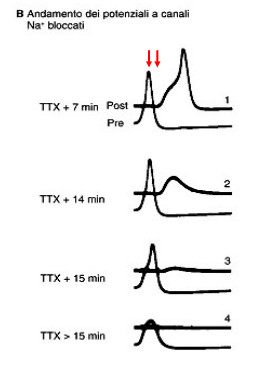
\includegraphics[scale=0.5]{immagine/sinapsi_gigante.jpg}
\caption{Trattamento con TTX}
\end{figure}

Il potenziale post sinaptico inizia ad avere un valore accettabile intorno ai 30-40 mV per quello presinaptico. Il grafico è un'esponenziale.

\paragraph{Placca motrice}
Regione di un motoneurone che perde la guaina mielinica e suddivide l'assone in vari rami che presentano \emph{varicosità}; in ogni varicosità di osserva un'indentazione della membrana sinaptica. 

Il terminale presinaptico è popolato di \emph{vescicole}. Se marchiamo con anticorpi che riconoscono i \emph{canali voltaggio dipendenti per il calcio}, li troviamo in vicinanza delle zone attive, che presentano invaginazioni della membrana postsinaptica. I recettori per l'\emph{acetilcolina} si trovano nella regione della membrana giunzionale, dove non ci sono i recettori si chiama regione extragiunzionale.

Mettiamo un elettrodo in vicinanza della membrana post sinaptica, che non entra nella membrana, ed una pipetta riempita con Ca. Se facciamo uscire una corrente da questa pipetta, esce calcio \lfreccia \emph{iontoforesi}. Mettiamo una coppia di elettrodi stimolanti per stimolare l'assone presinaptico ed un elettrodo nella membrana post-sinaptica. Stimoliamo il nervo ed otteniamo un'appena apprezzabile depolarizzazione (siamo in una soluzione con bassa concentrazione di $Ca^{2+}$).

Se stimoliamo + estrusione di $Ca^{2+}$, la stimolazione aumenta più $Ca^{2+}$ faccio uscire. Deve quindi essere presente $Ca^{2+}$ nel liquido extracellulare.


\paragraph{}
Per deprimere la funzionalità della sinapsi chimica, possiamo sostituire al $Ca^{2+}$ il $Mg^{2+}$. $Ca^{2+}$ è quindi essenziale per produrre la trasmissione sinaptica.

(16.12.2014)

Due elettrodi di voltaggio ed uno di corrente \lfreccia voltage clamp della membrana presinaptica: riusciamo a misurare le correnti nella membrana presinaptica. Quando il terminale viene invaso da un potenziale d'azione, si hanno correnti di Na e K.

In presenza di TTX e TEA, se evochiamo l'eccitazione della membrana presinaptica, le correnti di Na e K vengono bloccate. La presenza di TTX impedisce che la membrana post sinaptica (dove abbiamo un elettrodo) superi la soglia. Se riportiamo i potenziali di comando imposti alla membrana postsinaptica, vediamo nel terminale presinaptico delle correnti residue, che hanno una cinetica molto simile (anche se ribaltate in termini di polarità) alle correnti di K \lfreccia cinetica lenta: sono \emph{correnti di $Ca^{2+}$}.

La necessità di $Ca^{2+}$ extracellulare è importante per lo stabilirsi della corrente nel terminale presinaptico. Il fatto che se depolarizzo mi aumenta la corrente di $Ca^{2+}$, significa che i canali voltaggio dipendenti per il $Ca^{2+}$ si aprono. L'ampiezza delle correnti Na e l'ampiezza del potenziale post-sinaptico sono correlate: il terminale presinaptico, oltre alle correnti Na e K, è interessato anche da correnti \emph{voltaggio dipendenti} di $Ca^{2+}$.

\paragraph{Perchè l'assenza o la bassa concentrazione di $Ca^{2+}$ blocca il potenziale post-sinaptico?}
Queste correnti riescono ad elevare la concentrazione intracellulare del terminale. Si mette in evidenza utilizzando \emph{indicatori per il $Ca^{2+}$}, che hanno una $K_{S}$ elevata, ad esempio la \emph{fotoproteina,} in particolare l'\emph{aquorina}, estratta dai celenterati. 

\begin{figure}[H]
\centering
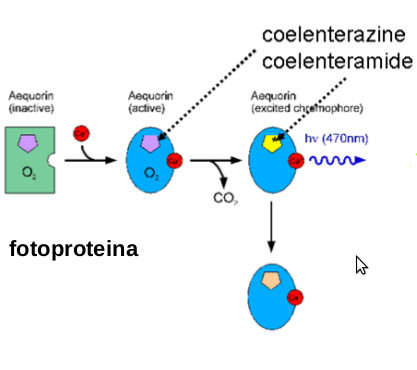
\includegraphics[scale=0.5]{immagine/fotoproteina.jpg}
\caption{Azione della fotoproteina nel legame con il $Ca?{2+}$}
\end{figure}
Il $Ca^{2+}$ permette che \emph{il gruppo prostetico della proteina venga perossidato}: questa condizione molecolare è lo \emph{stato attivo}, che decade allo stato inattivo emettendo fotoni a$\lambda$ 470 nm. Mettiamo tutto sotto un microscopio a fluorescenza: rappresentiamo le intensità di emissione con vari colori, dove verso il blu abbiamo le emissioni più basse ed in rosso quelle più alte. Quanto più $Ca^{2+}$ è presente, tante piu aquorine rilasciano fotoni, cioè un'elevazione di concentrazione intracellulare di $Ca^{2+}$.

\subsubsection{Ruolo del $Ca^{2+}$}
Il complesso sinaptico ha proteine specifiche, \emph{V-SNARE} e \emph{T-SNARE}, queste ultime ancorate alla membrana terminale. Nella zona attiva della sinapsi, le vescicole sono in equilibrio continuo tra alcune legate al citoscheletro ed altre che se ne distaccano ed iniziano ad aderire a regioni prossime alla membrana. Nei complessi proteici importanti per queste operazioni di attracco e ormeggio, c'è un \emph{canale ionico per il $Ca^{2+}$}: sono localizzati proprio in corrispondenza delle zone attive della membrana presinaptica. L'ingresso di calcio è cruciale per l'ultima fase, che vede la vescicola già attraccata al complesso della membrana target, che apre un varco di membrana e il contenuto della vescicola fuoriesce e diffonde.

Diverse tossine bloccano questi processi di trasmissione sinaptica.

\subsubsection{Sinapsi neuromuscolare}
A partire da Acetil-CoA e colina viene sintetizzata \emph{acetilcolina}, che viene incorportata nelle vescicole. Nel momento in cui la depolarizzazione provoca aumento dell'entrata di $Ca^{2+}$ nel terminale presinaptico, aumenterà la concentrazione di acetilcolina riversata nel vallo sinaptico.

L'acetilcolina agisce sui recettori post-sinaptici (hanno siti per legarla transitoriamente) e dopo viene rapidamente idrolizzata: la sua inattivazione avviene ad opera dell'\emph{acetilcolina esterasi}, enzima che si trova nel vallo sinaptico \lfreccia la colina viene recuperata ed internalizzata nel terminale presinaptico.

\paragraph{Acetilcolina esterasi}
Essenziale per l'\emph{interruzione del segnale}. Per l'interruzione concorrono due fenomeni:
\begin{enumerate}
\item{La depolarizzazione presinaptica, una volta manifestatasi, si esaurisce \lfreccia fenomeno secretorio acuto nella fase di depolarizzazione e che ricade in quella di polarizzazione. Ciò non basta per bloccare il segnale perchè il vallo sinaptico è piccolo e la concentraizone di acetilcolina sarebbe ancora elevata da permettere il legame successivo sui recettori}
\item{Azione dell'acetilcolina esterasi. Se essa non idrolizza l'acetilcolina, questa continua a restare legata ai recettori ed il sistema permane nello stato eccitato}
\end{enumerate}

\subsubsection{Recettore Acetilcolina}
Nelle pliche della membrana post-sinaptica abbiamo agglomerati di recettori per l'acetilcolina. La loro presenza sulla membrana post-giunzionale che guarda il terminale presinaptico in modo così addensato impedisce l'inserimento di altre proteine (sul resto della membrana invece ce ne sono meno).

È un \emph{pentamero}: subunità $\alpha$ (2, legano l'acetilcolina), $\beta$ $\gamma$ $\delta$.

Questi canali possono essere sottoposti ad una cinetica di questo tipo: vedi slides.

La transizione da legato chiuso a legato aperto è regolata da due \emph{costanti di probabilità} $\alpha$ e $\beta$. Questi recettori sono di tipo \emph{ionotropici} (ovvero sono anche canali ionici). La costante $\alpha$ indica la velocità di legame dell'agonista, ovvero la velocità di attivazione; la costante $\beta$ ci dice della cinetica di inattivazione. Conoscendole, giustifichiamo il decorso temporale di una corrente macroscopica.

TTX e TEA sono inefficaci su questi canali, mentre la \emph{bungarotossina} li blocca.

Questo canale non distingue granchè tra i cationi, passano più o meno tutti (Na, K, Ca). Quando il canale si apre, contemporaneamente attraverso il varco (non molto ristretto) passano gli ioni. Il flusso di Na e K è opposto: Na entra e la corrente è molto intensa, poichè il Na è ben lontano dal suo potenziale di equilibrio, mentre K esce, ma in modo meno violento. Il Ca entra in modeste quantità perchè la permeabilità è bassa \lfreccia il risultato è una \emph{depolarizzazione}.

Il fatto che il flusso di Na e K sia \emph{simultaneo} implica che manchi una condizione (sfasamento delle correnti) per realizzare un segnale di tipo tutto o nulla: si produce un \emph{evento graduato}. Tanto più sono aperti i canali, tanto più sarà depolarizzata la membrana post-sinaptica.

A questi recettori si associa un complesso di proteine, il \emph{complesso della Distrofina}: esse sono disposte a realizzare una connessione diretta meccanica tra lo spazio extracellulare ed il citoscheletro. Questo complesso protegge la membrana, scarica l'energia degli stress meccanici prodotti dalla fibra muscolare sui componenti extracellulari e citoscheletrici. Quando alcuni di questi elementi vengono alterati, si ha la \emph{distrofia}, una più o meno grave forma.

Questa sinapsi (neuromuscolare) è \emph{ad alto guadagno}, ovvero il potenziale d'azione è sempre così ampio da superare la soglia. In presenza di \emph{curaro}, possiamo far si che il numero di recettori disponibile per il legame dell'acetilcolina diminuisca in modo da produrre comunque un potenziale d'azione che però non raggiunge la soglia. La loro chiusura è scaglionata nel tempo!

\paragraph{Esperimento}
Per definire quali correnti vengono prodotte sulla membrana postsinaptica, mettiamo il voltage clamp nella post sinaptica ed un elettrodo nella presinaptica.

Stimolando, mantenendo il potenziale di membrana post sinaptico, registreremo un potenziale post sinaptico. Se spostiamo questo potenziale in senso depolarizzante o iperpolarizzante prima di stimolare: se iperpolarzziamo, l'ampiezza della depolarizzazione cresce, se facciamo il contrario decresce:

\begin{figure}[H]
\centering
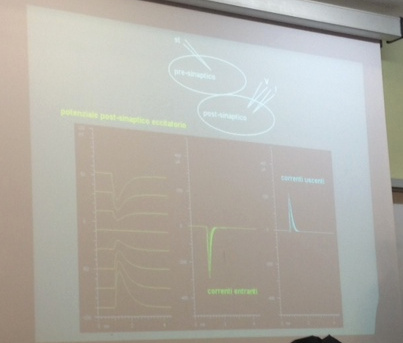
\includegraphics[scale=0.6]{immagine/esperimento.jpg}
\caption{Boh! Che ci scrivo???} 
\end{figure}

Ciò dipende dal fatto che i canali nel terminale presinaptico dipendono dal voltaggio! Tanto più ci allontaniamo dal potenziale $E_{Na}$, tanto più sodio entrerà.

A 0 questo segnale si annulla perchè man a mano che depolarizziamo, aumentiamo la corrente K e diminuiamo la corrente Na: nei pressi di 0 le due correnti sono identiche e quindi la variazione di potenziale è nulla. Questo ci dice qual è il \emph{valore di inversione}: queste correnti sono cationiche, perchè devono azzerarsi proprio nei pressi del valore di potenziale 0.

Se chiudiamo il circuito voltage clamp, la corrente netta di Na (entrante) prevale se l'impulso è depolarizzante mentre prevale quella di K (uscente) se l'impulso è iperpolarizzante.

Nelle condizioni fisiologiche abbiamo una \emph{depolarizzaizone}.

\paragraph{}
Il potenziale graduato decade in ampiezza lungo la fibra: il potenziale di placca non può infatti inluenzare sarcomeri diversi da quelli vicini alla regione della placca.

È lo stesso discorso della costante di spazio: osserviamo una corrente netta entrante di Na, che attraversa la membrana attraverso canali passivi. Tanto più canali passivi ci sono, tanto minore è la resistenza della membrana, tanto meno lontano andrà il potenziale.

Sia la placca motrice che la sinapsi neuromuscolare sono \emph{ad alto guadagno}, poichè la membrana extragiunzionale è caratterizzata da alta densità di canali Na voltaggio-dipendenti.

\paragraph{A che serve il potenziale d'azione nella fibra muscolare striata?}
Serve a generalizzare rapidamente la depolarizzazione sulla superficie dei sarcomeri. Più è veloce, più depolarizza la membrana in maniera pressochè sincrona in tutte le regioni. Se non ci fosse, l'attivazione si limiterebbe alle regioni prossime alla placca. In questo modo invece attiviamo i sarcomeri tutti insieme.

\subsubsection{Rilascio di vescicole}

I potenziali di placca sono eventi casuali. Se vediamo l'ampiezza del segnale, è inferiore al mV \lfreccia \emph{potenziali di placca in miniatura}. Che questi fossero legati all'azione dei recettori di acetilcolina ce lo dice il fatto che se applichiamo \emph{eserina}, che inbisce la colina esterasi, questi eventi diventano più ampi, ma anche più numerosi. Ciò avviene perchè, bloccando la colina esterasi, avremo un legame ripetuto sui recettori.

I recettori acetilcolina vengono cimentati anche in assenza di attività della membrana presinaptica! Questa sarebbe la dimostrazione che il neurotrasmettitore viene rilasciato anche senza stimolazione presinaptica. Il fatto che siano eventi discreti è stato assimilato al fatto che i recettori rispondano così rispetto al rilascio di acetilcolina nel vallo.

Se ciò fosse vero, dovevamo poter produrre un fenomeno scalare che fosse correlato col rilascio di numeri diversi di vescicole. 

In realtà i potenziali in miniatura possono esse prodotti in multipli.
\paragraph{Esperimento}
Mettiamo alto Mg e basso Ca, abbiassando il Ca che entra abbassiamo anche il numero di vescicole che si fondono \lfreccia distinguiamo tra numeri diversi di vescicole che si formano. Dò lo stimolo, ottengo diverse variazioni (vedi slides)(gli stimoli S sono spontanei). Infine prendo queste ampiezze e le distribuisco in un istogramma di frequenza: in ascissa la classe di ampiezza del potenziale di placca e in ordinata il numero di osservazioni che cadono nell'intervallo.

\begin{figure}[H]
\centering
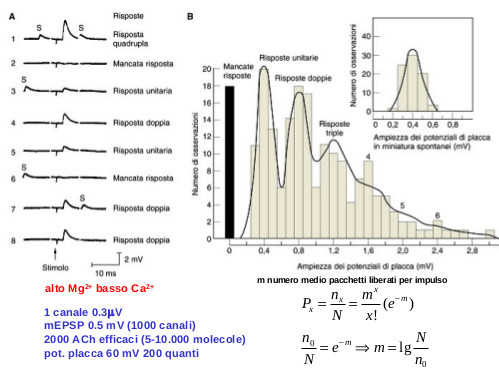
\includegraphics[scale=0.6]{immagine/poisson.jpg}
\caption{Distribuzione di poisson}
\end{figure}

 Avrò un gran numero di risposte mancate, mentre quelle non mancate si distribuiscono in modo simile alla \emph{distribuzione di Poisson}. 

Vediamo che i picchi di ampiezza (multipli) sono doppi, tripli, quadrupli di una risposta unitaria che ha il picco a 0,4 mV.

Anche l'ampiezza media picca a 0,4 mV. Perchè?

Ciò si spiega col fatto che il sito in cui il fenomeno si manifesta è a distanza variabile dall'elettrodo. Se un Meps è prodotto dall'apertura di una singola vescicola, quando le vescicole che si aprono in regime depresso è il doppio, ...?\todo{senti registrazione}.

È quindi plausibile l'ipotesi che un potenziale in miniatura sia prodotto ogni tanto dal rilascio di una vescicola.

Se la media di produzione di vescicole di condizioni di alto Mg e basso Ca è 0,4, potrò averne il doppio, il triplo ecc secondo la distribuzione di Poisson.

\emph{Il potenziale in miniatura è il seguito di un fenomeno sporadico di rilascio di vescicole (secrezione basale), che può essere moltiplicato per 200 dall'arrivo di un potenziale di azione.}

Il contenuto di acetilcolina per vescicola è tra 5000 e 10000 molecole.

(17.12.2014)

\subsection{Sinapsi centrali o neuroneuronali}
I bottoni sinaptici sui neuroni possono localizzarsi in vari punti.
\begin{itemize}
\item{Sinapsi asso-somatica: i terminali prendono contatto con la regione somatica}
\item{Sinapsi asso-dendritiche: si specializzano anche spine dendritiche sulle quali vanno a finire i terminali}
\item{Sinapsi asso-assonica}
\end{itemize}

Le sinapsi che poggiano sul soma hanno un effetto più ravvicinato rispetto a quelle che poggiano sul colletto assonico. 

Le asso-assoniche lavorano a valle del sito di inizio del potenziale di azione. Considerando che il neurone può avere vari rami assonici, è chiaro che questa sinapsi ha azione molto selettiva: modula di fatto solo determinati contatti che il neurone ha con il neurone a valle. Se fosse una sinapsi inibitoria presinaptica, solo la parte che contatta sarebbe inibita, il resto del neurone no. Operano su un sistema già attivo \lfreccia contatto modulatorio.

La vicinanza o lotananza di ciascun bottone rispetto al sito di inizio del potenziale di azione è importante: quelle più vicine al soma pesano di più.
\paragraph{Trasmissione}
L'informazione passa da un elemento eccitabile ad un altro.
\paragraph{Modulazione}
Fenomeno capace di \emph{aumentare o diminuire l'efficacia della trasmissione}. Prendiamo una fibra neuronale e la placca motrice: le fibre provengono da un motoneurone. Accanto ad esso ci sono vari assoni che provengono dal sistema nervoso autonomo ortosimpatico (varicosi), in cui i bottoni sono lontani fra loro rispetto alla classica sinapsi: produzione di \emph{noradrenalina} che agisce sia sul terminale del motoneurone che sulla fibra post-sinaptica aumentando l'efficacia della trasmissione del motoneurone sulla placca motrice.

\paragraph{}
Al cono d'emergenza arriverà un \emph{potenziale sottosoglia} \lfreccia no impulso. 

Se superata la soglia \lfreccia impulso. La soglia inizia a ridursi proprio nella regione d'emergenza, in cui si incrocia un'ampiezza del potenziale sinaptico utile a produrre un potenziale d'azione.

\subsubsection{Recettori eccitatori}
Rispondono al legame con Glu, Gly. Per la sinapsi eccitatoria del SNC abbiamo diversi tipi di recettori noti, due dei quali sono \emph{ionotropici} (sia sito di riconoscimento per neurotrasmettitore che canale ionico). Un terzo recettore è di tipo \emph{metabotropico}.
\paragraph{Recettore metabotropico}
Associato ad una G proteina che opera su un enzima modificatore. Questo, quando lega il Glu cambia conformazione, cambia anche la G proteina che si dissocia ed attiva la fosfolipasi PLC che produce due secondi messaggeri: inositolo 3 P(capace di agire su canali per Ca collocati sul reticolo endoplasmico, li apre ed esce calcio) e DAG.

La funzione ionotropica è affidata ai canali di Ca.

\paragraph{Recettore ionotropico}
Due tipi:
\begin{enumerate}
\item{Non-NMDa}
\item{NMDA: ammette flussi ionici maggiori quando aperto. Fa passare anche discrete quantità di $Ca^{2+}$. Hanno un sito per Mg (circa a metà del canale): esso disturba solitamente i flussi ionici perchè entra nel canale dall'esterno, ma non può passare \lfreccia blocca il flusso di ioni. }
\end{enumerate}

Quando c'è Glu, entrambe i canali legano l'agonista ed aumentano la probabilità di aperturta, ma Non-NMDA si apre subito, mentra l'altro no perchè alloca Mg nel sito. Se facciamo una stimolazione breve presinaptica, la corrente passa prevalentemente attraverso i canali Non-NMDA. I canali NMDa possono essere attivati:
\begin{enumerate} 
\item{se l'eccitazione presinaptica dura nel tempo: i flussi cationici depolarizzano la membrana e il Mg viene sputato fuori}
\item{Se sulla membrana post-sinaptica agiscono altre sinapsi che hanno già depolarizzato la membrana}
\end{enumerate}

Sono quindi dei \emph{rafforzatori della risposta}.

Mentre il sistema sinaptico neuromuscolare prevede solo l'eccitazione, nel SNC esiste uno spegnimento del segnale. Ci sono vari tipi di canali che provvedono a questa inibizione.
\subsubsection{Sinapsi inibitoria}

Canali permeabili al cloro e recettori per il neurotrasmettirore GABA: Cl entra iperpolarizzando la membrana \lfreccia allontanamento dalla soglia \lfreccia inibizione della struttura post-sinaptica.

Alcuni recettori rispondono a neurotrasmettitori inibitori aprendo i canali per K+.


Una corrente entrante depolarizzante viene dispersa attraverso i canali passivi e ne arriva un residuo che, se superiore alla soglia, innesca il potenziale d'azione. Una sinapsi inibitoria comporta un \emph{allontanamento dalla soglia}. Questo se si ha un potenziale prodotto da un solo stimolo presinaptico.

\paragraph{Cosa accade se si hanno più potenziali d'azione in successione?}
Il potenziale presinaptico è breve e tutto o nulla, quello post sinaptico è più lungo (10 ms) e graduato. Se faccio un altro potenziale d'azione presinaptico che abbraccia la durata del primo potenziale post-sinaptico, non ne vedrò effetto. Se però ne faccio un altro più ravvicinato, di durata minore rispetto al primo potenziale post-sinaptico, avrò una \emph{sommazione}. 

Il grado di sommazione se stimolo due volte un ingresso sinaptico è dato dalla costante di tempo della membrana post-sinaptica: tanto più è elevata, tanto più grande sarà la sommazione \lfreccia \emph{sommazione temporale}.

Analogamente, se ho due ingressi sinaptici separati e li attivo in modo ravvicinato, più grande sarà la costante di spazio e più avrò sommazione (\emph{sommazione spaziale}).

\subsubsection{Rilascio vescicole}
Si ha un bilanciamento di aggiunta di membrana (\emph{esocitosi del neurotrasmettitore}) e recupero (\emph{endocitosi clatrina-mediata}).

Il contenuto della vescicola viene secreto, ma a seconda dell'invaginaizone che si forma, quello che è presente all'esterno della membrana viene internalizzato: la presenza di fattori trofici o molecole che hanno importanza nel decidere di una popolazione di cellule in differenziamento quali rimarranno e quali resteranno indifferenziate (sagomatura), fa si che si scelga una delle due vie. Se un terminale è attivo e secerne molto, internalizzerà molto. 

\subsubsection{Neurotrasmettitore}
Per definire una sostanza \emph{neurotrasmettitore}, deve avere 4 caratteristiche:
\begin{enumerate}
\item{RNA legato alla sintesi del trasmettitore}
\item{Vederlo nelle vescicole presinaptiche}
\item{Recettori specifici per il neurotrasmettitore}
\item{Riconoscere gli attori dell'espressione dei neurotrasmettitori}
\end{enumerate}

Ci sono neurotrasmettitori responsabili non solo della trasmissione, ma anche della modulazione, come le \emph{neuroendorfine}, sostanze peptidiche rilasciate da alcuni terminali del SNC che attivano recettori che possono essere attivati anche da sostanze psicoattive.

Un terminale polinergico rilascia acetilcolina e ATP: ATP viene idrolizzato \lfreccia adenosina. Esistono recettori nel terminale per l'adenosina: la loro attivazione comporta la riduzione della quantità di vescicole rilasciate per ogni impulso \lfreccia \emph{autoregolazione} quando la secrezione è eccessiva, il sistema la spegne (\emph{feedback negativo}).

Terminali di tipo varicoso hanno delle varicosità sull'assone, ma accade la stessa cosa che nei polinergici.

\subsubsection{Funzione della Glia}
Il numero di variabili in base alle quali può funzionare una sinapsi cerebrale è enorme! Possono esserci moltissimi stati funzionali per il sistema nervoso.

La glia \emph{collabora tra funzione presinaptica e postsinaptica}: il Glu sintetizzato nel terminale viene rilasciato e ricaptato. Parallelamente il trasportatore per il glu si trova anche sulla cellula gliale: prende Glu, lo modifica il Gln e la cede al terminale, che la riutilizza per la sintesi di Glu. Consideriamo che rispetto all'informaizone nervosa, molto rapida, nella glia ci sono fluttuaizoni della concentrazione di $Ca^{2+}$ molto lente, che hanno quasi la caratteristica di impulsi rallentati \lfreccia la trasmissione sinaptica opera su un tempo breve, e potrebbe esistere una forma ecofunzionale per cui lo stato della glia attorno condizionerebbe la trasmissione.

(16.02.2015)

\section{Canali ionici}
È importante conoscere le proprietà de icanali ionici per le malattie genetiche e perchè è la base per la farmacologia, in modo da trovare farmaci che agiscono dove devono agire con il minor quantitativo di effetti indesiderati.

\subsection{Ipotesi di lavoro di canale ionico}
Attraverso lo strato lipidico  una molecola integrale di membrana si situa a tutto spessore. Essa possiede due gruppi di domini:
\begin{itemize}
\item{Sequenze di aa lipocompatibili : non presentano cariche, si interfacciano bene con la parte lipidica}
\item{Sequenze di aa che sono in buon \emph{equilibrio termodinamico} avendo contatto con acqua}
\end{itemize}

\paragraph{Canale ionico} dispositivo della membrana capace di realizzare un poro persistente acquoso, sempre riempito di acqua e ioni, guardato da \emph{cancelli}.
\begin{figure}[H]
\centering
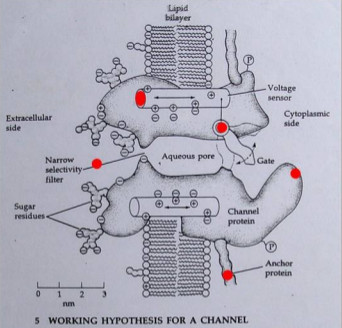
\includegraphics[scale=0.5]{immagine/canali.jpg}
\caption{Rappresentazione di un canale ionico}
\end{figure}

Il versante extracellulare vede gruppi \emph{glicidici}\footnote{i canali sono glicoproteine}, che affacciano verso la parte esterna della membrana. Sono importantissimi come codice di riconoscimento tra le cellule e sono alla base di molti dei fenomeni di \emph{compatibilità} fra tessuti e cellule, così come sono dei siti per il riconoscimento dei canali attraverso la tecnica degli anticorpi.

La parte esterna vede un \emph{vestibolo}, una regione di accesso che ioni extracellulari devono impegnare ancor prima di accedere al vero e proprio canale. Ce n'è uno anche nella parte intracellulare: queste due regioni non sono necessariamente equivalenti per i vari ioni. Questo è alla base del fenomeno di \emph{rettificazione} : passaggio di ioni meglio in una direzione che in quella opposta\footnote{vedi prossima lezione}. 

In un certo punto del poro si delinea una regione, chiamata \emph{filtro di selettività}: è un filtro \emph{sterico}, basa la sua proprietà di filtraggio sull'ingombro che le specie ioniche hanno. I canali ionici sono attraversati da ioni molto diversi ed in condizioni diverse: alcuni ioni attraversano il canale con il \emph{mantello di idratazione} che circonda ogni ioni quando si trova in soluzione, a volte invece devono perderlo e passare come \emph{ioni nudi}.

Il filtro sterico però non basta: in questo modo infatti non si avrebbe selettività per ioni grandi\footnote{Se un setaccio fa passare ioni grandi, passano anche quelli più piccoli}. Il filtro di selettività è quindi caratterizzato anche dalla presenza di \emph{cariche fisse}, disposte singole o in coppia: operano un'ulteriore selettività. 

In base a caratteristiche steriche e di carica, ogni canale accetta alcuni ioni si ed altri no.

Le parti nella regione intracellulare hanno vari domini interessanti:

\begin{itemize}
\item{Siti di attacco per proteine ancoranti : la potenzialità di movimento di una molecola glicoproteica una volta inserita nella membrana si ha lateralmente. Se solo questo fenomeno fosse possibile, si avrebbe una distribuzione ubiquitaria dei canali, ma i canali ionici non sono distribuiti ubiquitariamente. L'interazione tra parti intracellulari del canale ionico e proteine che prendono legame con \emph{elementi citoscheletrici}, e che riconoscono singolarmente le categorie di canali ionici, permette la distribuzione specifica dei vari canali}
\item{Regioni che espongono residui di Ser e Tre, che possono essere fosforilati dalle \emph{protein chinasi A e C}. La fosforilazione del canale equivale al fenomeno di fosforilazione di un enzima: il substrato è lo ione nel versante extracellulare e il prodotto è la traslocazione dello ione nel lato opposto (o viceversa). La funzione del canale ionico è fortemente legata allo stato di fosforilazione/defosforilaizone del canale stesso}
\item{Regioni che presentano un appendice che può essere spostata in chiusura: un \emph{cancello} è il dispositivo che mima il fenomeno di transizione apertura/chiusura. La natura transizione prescinde dalla presenza di uno stimolo: i canali hanno una cinetica molecolare per cui alternano cambi conformazionali che portano allo stato percorribile, a situazioni in cui il canale non è conduttivo. Di solito si ha un solo cancello, a volte anche altri domini della molecola collaborano}
\end{itemize}
Nei canali passivi non ci sono sensori per il voltaggio, nei voltaggio dipendenti si. Ci sono \emph{zone recettoriali} per i canali chimicamente controllati; una regione sensibile alle variazioni di tensione che la membrana riceve nei canali meccanocettori.

\paragraph{Qual è la relazione tra sensore e cancello?}
Nei canali passivi non c'è: la responsabile di apertura e chiusura è l'\emph{agitazione termica}. Ciò può essere alterato dalla presenza dei sensori: i sensori trasducono lo specifico stimolo che controlla la cinetica di \emph{quel} canale ionico, ma la cinetica di base è una proprietà generale di tutti.

Designamo come cancello una regione che può avere due posizioni: una aperta ed una chiusa. In realtà cambi di conformazioni tra aperte e chiuse interessano una larga parte della molecola, non solo quella relativa al cancello.

Applicando le tecniche del voltage clamp abbiamo isolato correnti macroscopiche e abbiamo teorizzato il funzionamento dei canali Na. 

\subsection{Come studiamo un canale ionico?}
Applicando le tecniche di voltage clap siamo stati in grado di isolare le correnti macroscopiche e porre in atto una teorizzazione del funzionamento dei canali.

I canali possono essere studiati grazie a 2 avanzamenti tecnologici:
\begin{enumerate}
\item{Patch clamp. Patch = tassello (di membrana) e clamp = controllo}
\item{Cloning, purificazione, espressione}
\end{enumerate}
L'accoppiamento tra questi due indirizzi (elettrofisiologia molecolare e biologia molecolare) ha aiutato.

\paragraph{Come rappresentiamo un canale ionico?}
Il liquido intracellulare contiene varie specie ioniche, quello extracellulare anche: un canale selettivo per K sarà attraversato solo da K. Troviamo così una specificità per i vari canali \lfreccia selettività della membrana. Abbiamo potuto fare lo schema elettrico della membrana in cui mettevamo in parallelo le varie vie di corrente perchè abbiamo molecole che passano da una parte all'altra. Se non ci fosse questprincipio di selettività, non ci sarebbe potenziale di azione.

Rappresentiamo una resistenza, che è il reciproco della conduttanza del canale (es canale di K), ed una batteria, che è la stessa per ogni canale.

Indichiamo la conduttanza elementare come $\gamma_{k}$, la corrente elementare attraverso un canale come $i_{k}$, e la foza elettromotrice è ($V_{m} - E_{k}$):
\begin{figure}[H]
\centering
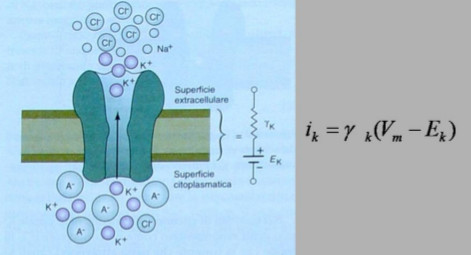
\includegraphics[scale=0.4]{immagine/potassio1.jpg}
\caption{I canali permeabili selettivamente agli ioni $K^{+}$ danno origine ad una forza elettromotrice pari al potenziale di Nernst per i $K^{+}$}
\end{figure}
 
\subsubsection{Patch clamp}
Elettrodi non ad ago\footnote{apertura 100 nm}, ma \emph{conici}:l'apertura è intorno ad 1 $\mu m$. Questi elettrodi possono essere costruiti con vetri particolari, che hanno grossa affinità per il doppio strato lipidico\lfreccia adesione.

Gli elettrodi sarebbero taglienti lungo il margine del distacco, ma vengono arrotondati con un procedimento termico. Essi \emph{poggiano} sulla membrana, non vi penetrano.

Man a mano che l'elettrodo si avvicina alla membrana, misura la resistenza che la membrana offer. La corrente esce liberamente dall'elettrodo, che inzialmente ha una resistenza di 4 $M\Omega$; avvicinandosi,lo spazio di fuga della corrente si riduce e la resistenza aumenta; poi la membrana viene portata a contatto \lfreccia \emph{suzione} \lfreccia la resistenza diventa 1 $G\Omega$.

Se la corrente attraversa la membrana e contatto tra vetro e membrana è piccolo, gran parte di essa entra nella pipetta.
Nel tassello delimitato dalla pipetta a contatto con la membrana c'è un canale ionico attraversato da una corrente, la quale può percorrere la pipetta o essere dispersa. Se quest' ultima via è stretta, gran parte della corrente viene raccolta nella pipetta, dove c'è un elettrodo metallico: questo contatto entra in un circuito, detto \emph{convertitore corrente-voltaggio}, che converte la corrente in un segnale di voltaggio, che può essere letto su un oscillografo.
È un circuito a basso rumore, legge valori di correnti fino a $10^{-12}$ ampère. La batteria mi permette di applicare una ddp tra l'interno della pipetta e l'esterno del bagno: si realizza il fissaggio della tensione tra esterno ed interno della pipetta, ecco perchè si chiama patch clamp.

La dimensione dell'apertura della pipetta e la \emph{densità di canali} nella regione di interesse influenza il numero medio di canali che la pipetta raccoglierà. Si può sagomare la pipetta per raccogliere un solo canale ionico.

\subsection{Come applichiamo questa tecnologia e cosa studiamo?}

\textbf{Cell-attached}: la pipetta è saldata alla membrana e si registra quello che fluisce tra citoplasma e tratto terminale della membrana. Studiamo il canale nella situazione nativa, in cui esso è in connessione con il  citoscheletro (importante per i canali meccanocettivi: avere un tirante nel citoscheletro ne amplifica infatti la sensibilità meccanica). Avere il contatto della proteina canale con un milieu interno ricco dei fattori che lo modulano è diverso dal registrare il canale in \emph{condizione isolata}.

\begin{figure}[H]
\centering
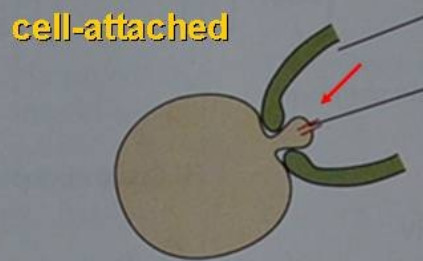
\includegraphics[scale=0.35]{immagine/cell.jpg}
\caption{Tecnica cell-attached}
\end{figure}

Dalla posizione cell-attached, la condizione isolata \textbf{inside out} si realizza tirando via la pipetta\footnote{l'interazione vetro-membrana è superiore a quella doppio strato-doppio strato}: portiamo via un tassello di membrana. 
\begin{figure}[H]
\centering
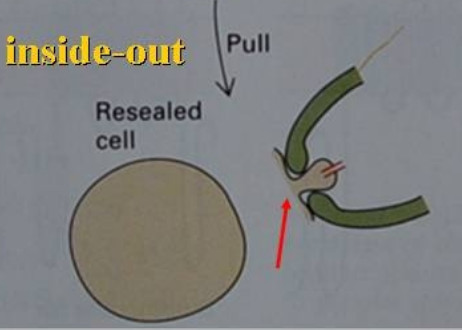
\includegraphics[scale=0.35]{immagine/inside.jpg}
\caption{Tecnica inside-out}
\end{figure}

La membrana si risalda e la parte interna della proteina è out, fuori dalla pipetta. Questa configurazione ci serve per studiare la dipendenza della funzione di una corrente dal pH o dalla concentrazione di Ca intracellulare. 
Farlo in condizione di cell-attached è molto complicato! In questa modalità invece presentiamo alla faccia interna del tassello una soluzione con le caratteristiche da noi desiderate, con varia composizione di pH e Ca. 

Partendo dalla configurazione cell-attached possiamo fare un'ulteriore suzione, rompendo il tassello, per ottenere la configurazione \textbf{whole-cell}: abbiamo accesso completo al citoplasma intracellulare. È una situazione simile al voltage clamp: la corrente che entra o esce dalla pipetta interessa \emph{tutti i canali della membrana}, non pochi come nelle altre due \lfreccia si leggono \emph{correnti macroscpiche}.

Il contenuto della pipetta può essere controllato che a causa della grossa apertura (più di 1 micron) può fluire nel citoplasma: la cellula viene \emph{dializzata}  In pochi minuti il citosol viene sostituito con contenuto della pipetta, che è molto maggiore in volume del citoplasma. Possiamo così studiare correnti macroscopiche e possono essere immesse delle chinasi, e quindi up-regolare il canale, oppure delle fosfatasi, e down-regolare \lfreccia leggiamo la corrente macroscopica controllando il citoplasma.

\begin{figure}[H]
\centering
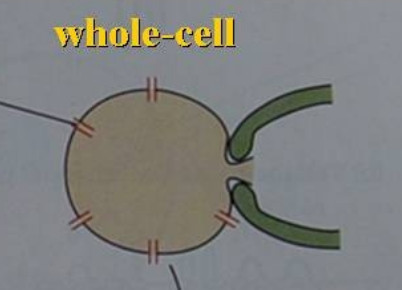
\includegraphics[scale=0.35]{immagine/whole.jpg}
\caption{Tecnica whole-cell}
\end{figure}

Se poi tiriamo via lentamente la cellula, abbiamo isolato un tassello, che però presenterà la parte extra-cellulare all'esterno della pipetta: \textbf{outside-out} (vedi foto su cell).
Come avviene? Quando partiamo da whole cell, se allontaniamo la pipetta, la membrana si tira e dilata e ad un certo punto del tiraggio la membrana \emph{collabirà}\footnote{afflosciare}, quindi la parte esterna alla pipetta sarà quella extracellulare. 

È possibile in questo caso studiare il canale per vedere se c'è un neurotrasmettitore che stimola il canale, quindi presentare diverse concentrazioni di agonista all'esterno della pipetta, mentre misuriamo l'attività del canale.

\begin{figure}[H]
\centering
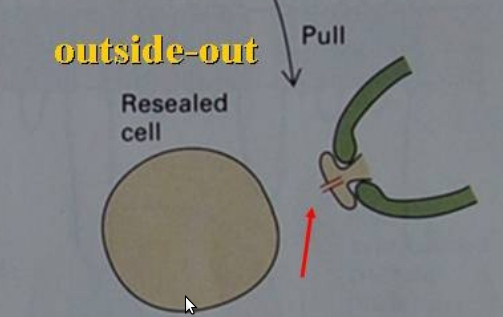
\includegraphics[scale=0.35]{immagine/out.jpg}
\caption{Tecnica outside-out}
\end{figure}

\subsubsection{Inside-out}
È la configurazione più facile per riconoscere le varie categorie di canali ionici.

Controlliamo la differenza tra il liquido nella pipetta e quello all'esterno, che sono isopotenziali. Il clamp di voltaggio riguarda quindi i potenziali ai due lati del canale ionico.

Ponendo una ddp tra quei due punti, possiamo calcolare la corrente come conduttanza di un certo ione moltiplicato per $V_{m}$ ed $E_{k}$:
\begin{figure}[H]
\centering
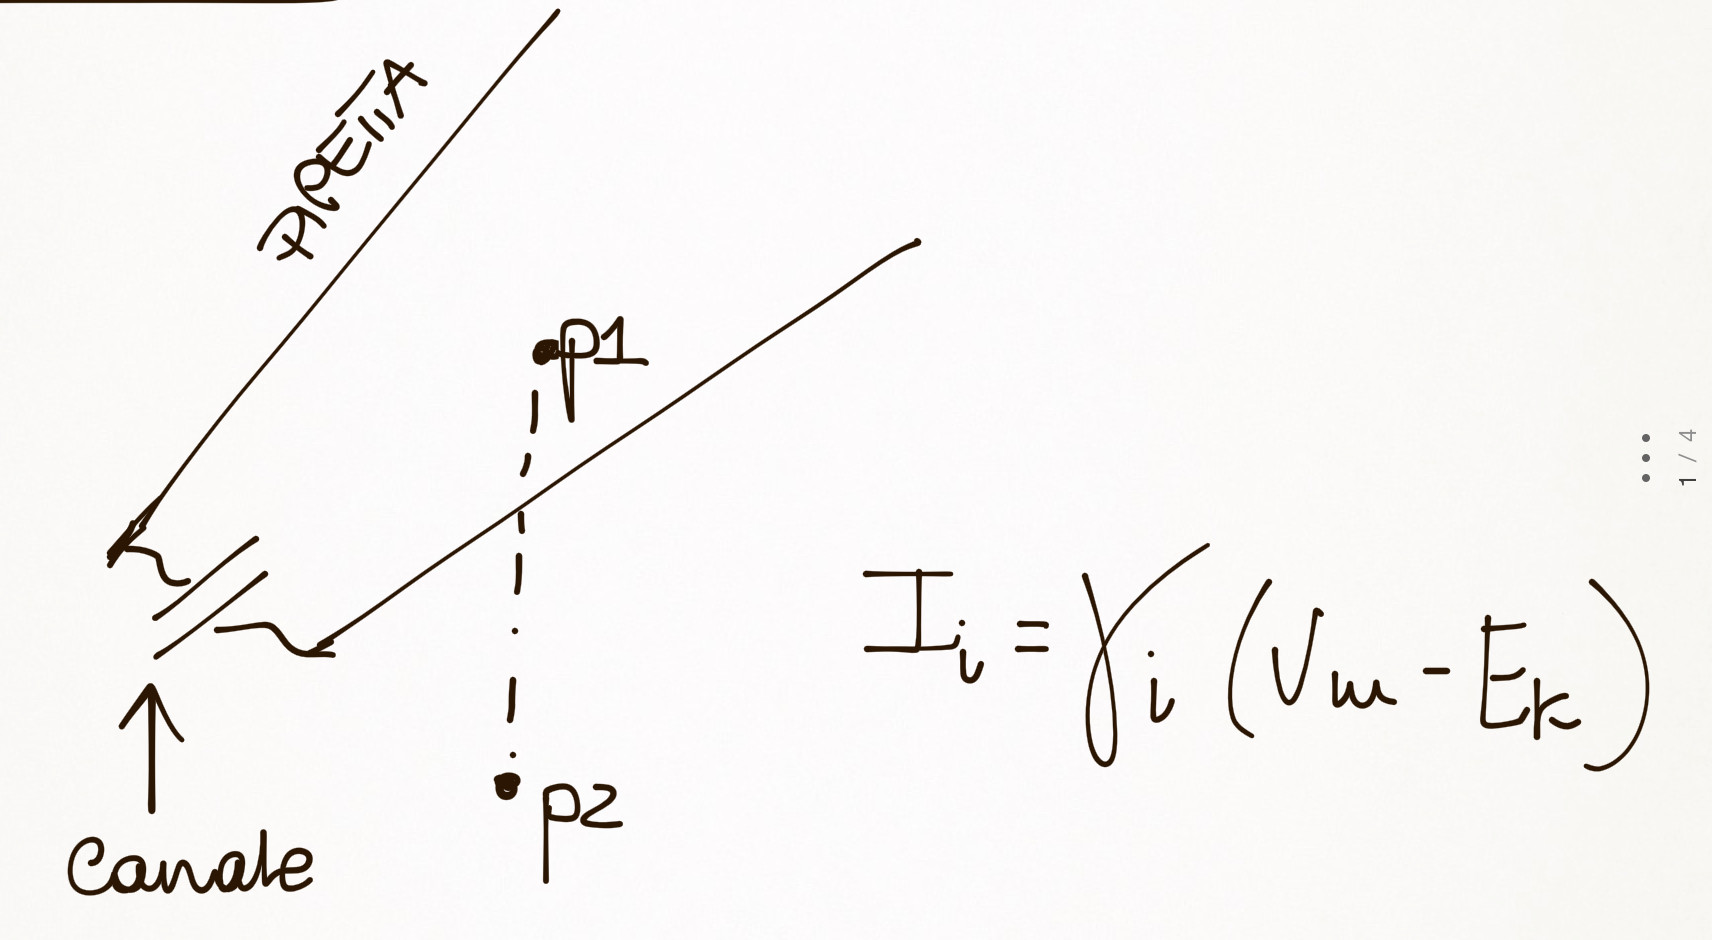
\includegraphics[scale=0.1]{immagine/1.jpg}
\end{figure}
Cosa osserveremmo all'oscillografo?

Come attività di un singolo canale ionco, la corrente balla fra due livelli. 

Se ce ne fossero più di uno, ci sarebbero più pianerottoli di corrente, perchè se metto in parallelo più conduttori dovrò avere salti multipli di corrente. Quando vediamo la corrente saltare da un livello all'altro, ciò appare rapidissimo nella scala temporale dei $\mu s$. Siccome i due livelli corrispondono allo stato \emph{conduttivo} e \emph{non conduttivo} del canale, il salto rapido indica che il cambio di conformazione avviene più velocemente dei $\mu s$. Considerando che le torsioni dei gruppi funzionali della molecola avvengono in ns, il canale, come un coltello a serramanico, se sollecitato può scattare in varie conformazioni. I cambi di conformazione sono molto rapidi e ci appaioni istantanei. Se così non fosse, vedremmo la corrente passare da chiuso ad aperto in molto tempo, e non riusciremmo a distinguere se uno o più canali si addizionano:
\begin{figure}[H]
\centering
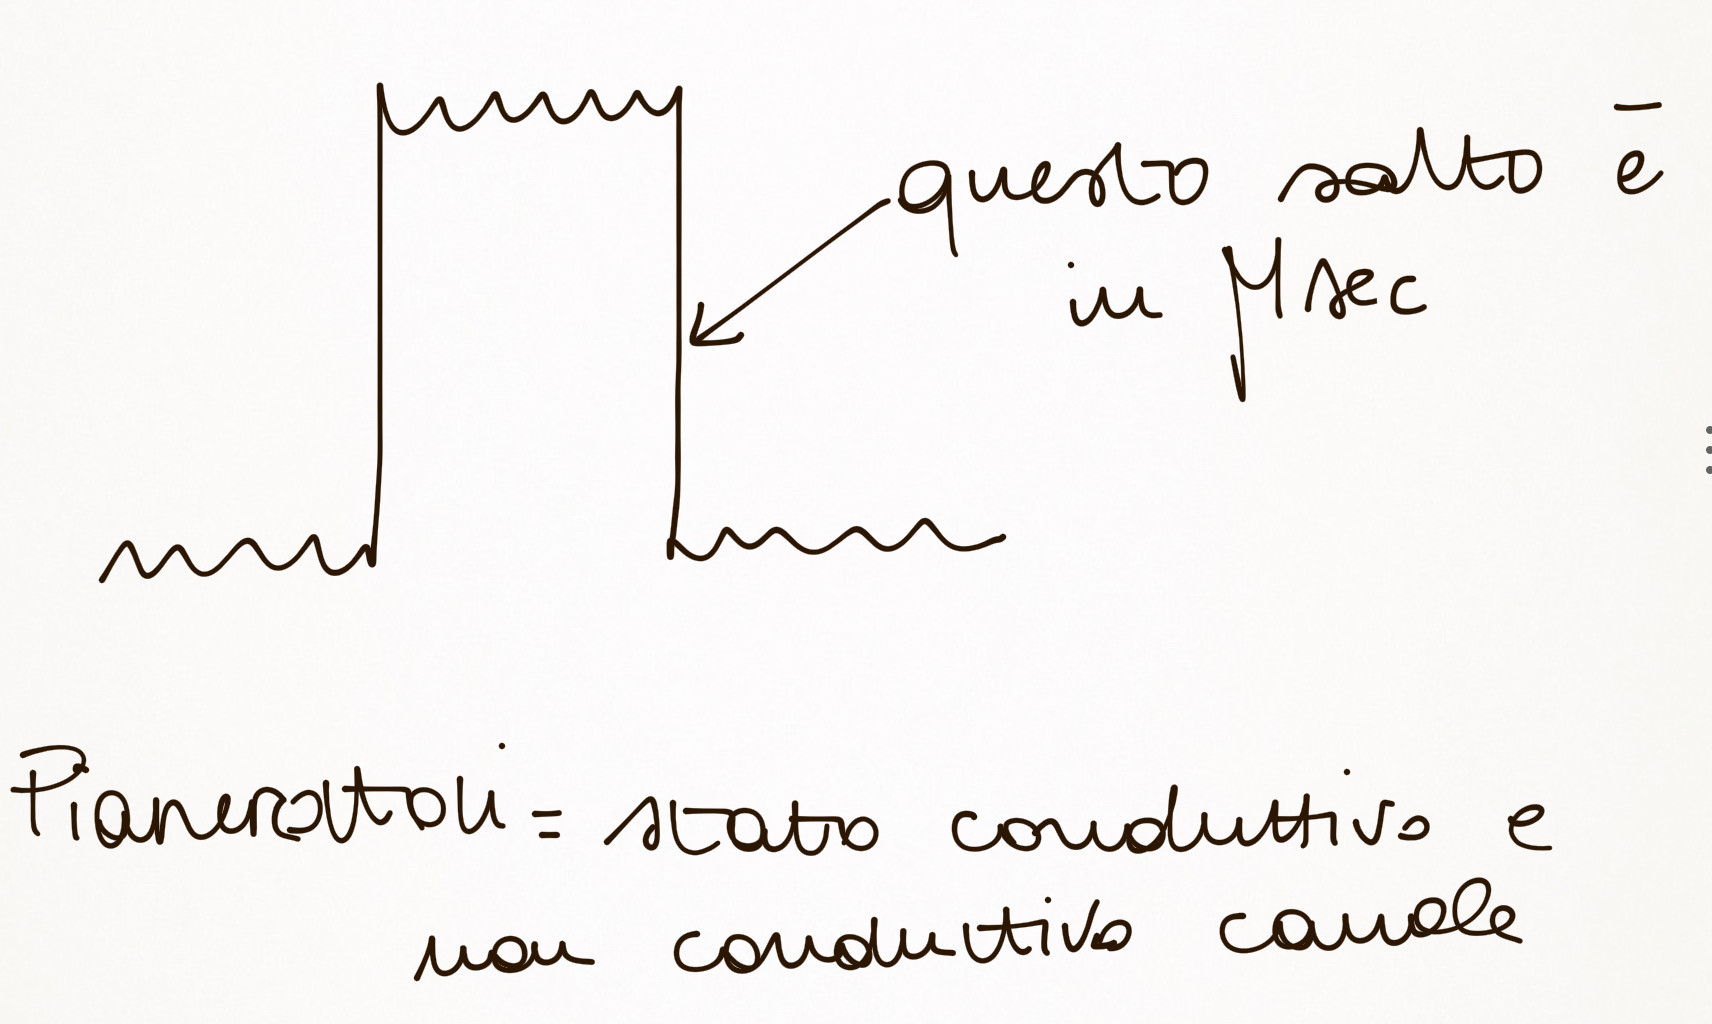
\includegraphics[scale=0.1]{immagine/2.jpg}
\caption{...}
\end{figure}

\paragraph{Rumore}
Varianza\footnote{differenza tra ogni punto e la media} intorno alla media. Il livello inferiore corrisponde al canale chiuso, ma quando ioni passano attraverso il canale fanno più \emph{rumore}, che è la variazione istante per istante degli ioni che stanno passando. Abbiamo tratti in cui passano più ioni e tratti in cui ne passano meno. 
\begin{figure}[H]
\centering
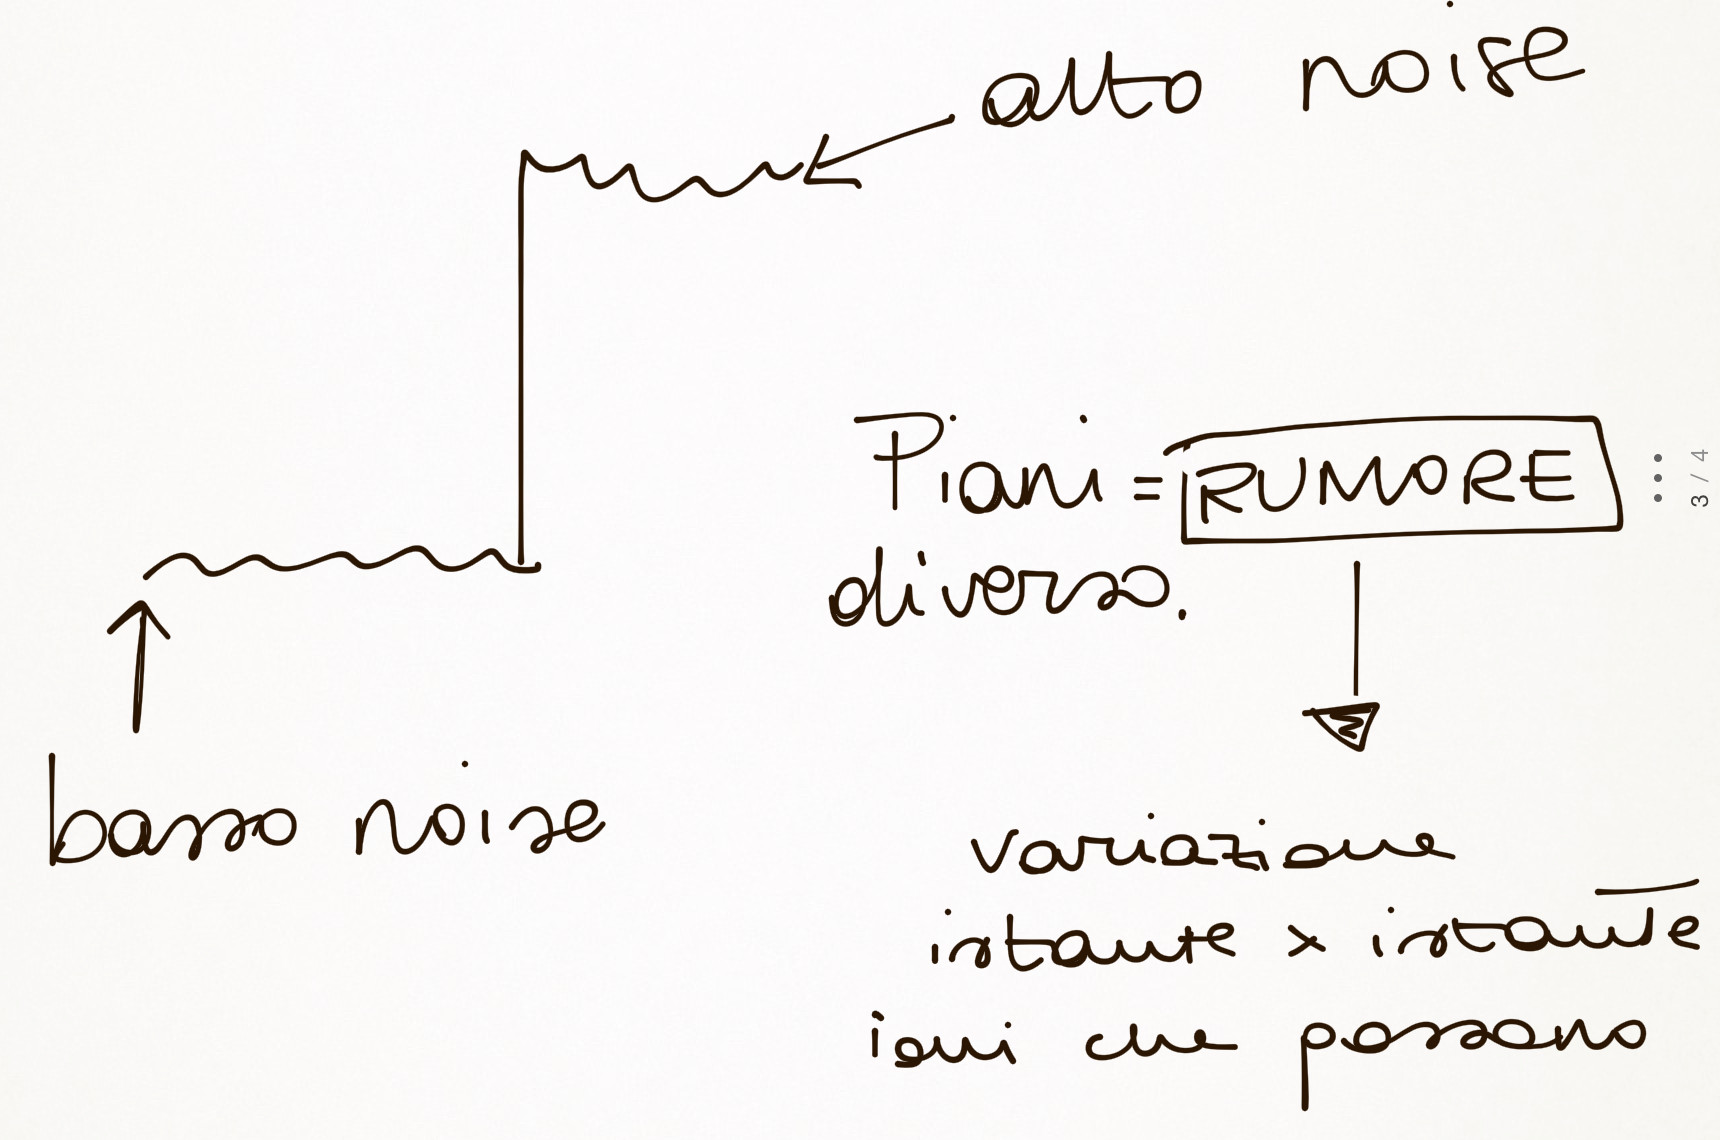
\includegraphics[scale=0.1]{immagine/3.jpg}
\caption{...}
\end{figure}

Ci sono intervalli chiusi brevi o lunghi: non c'è dipendenza tra quando si apre/chiude e dopo quanto tempo si chiude/apre \lfreccia \emph{fenomeno stocastico} o casuale, come prevede la \emph{teoria dell'agitazione termica}.

\begin{figure}[H]
\centering
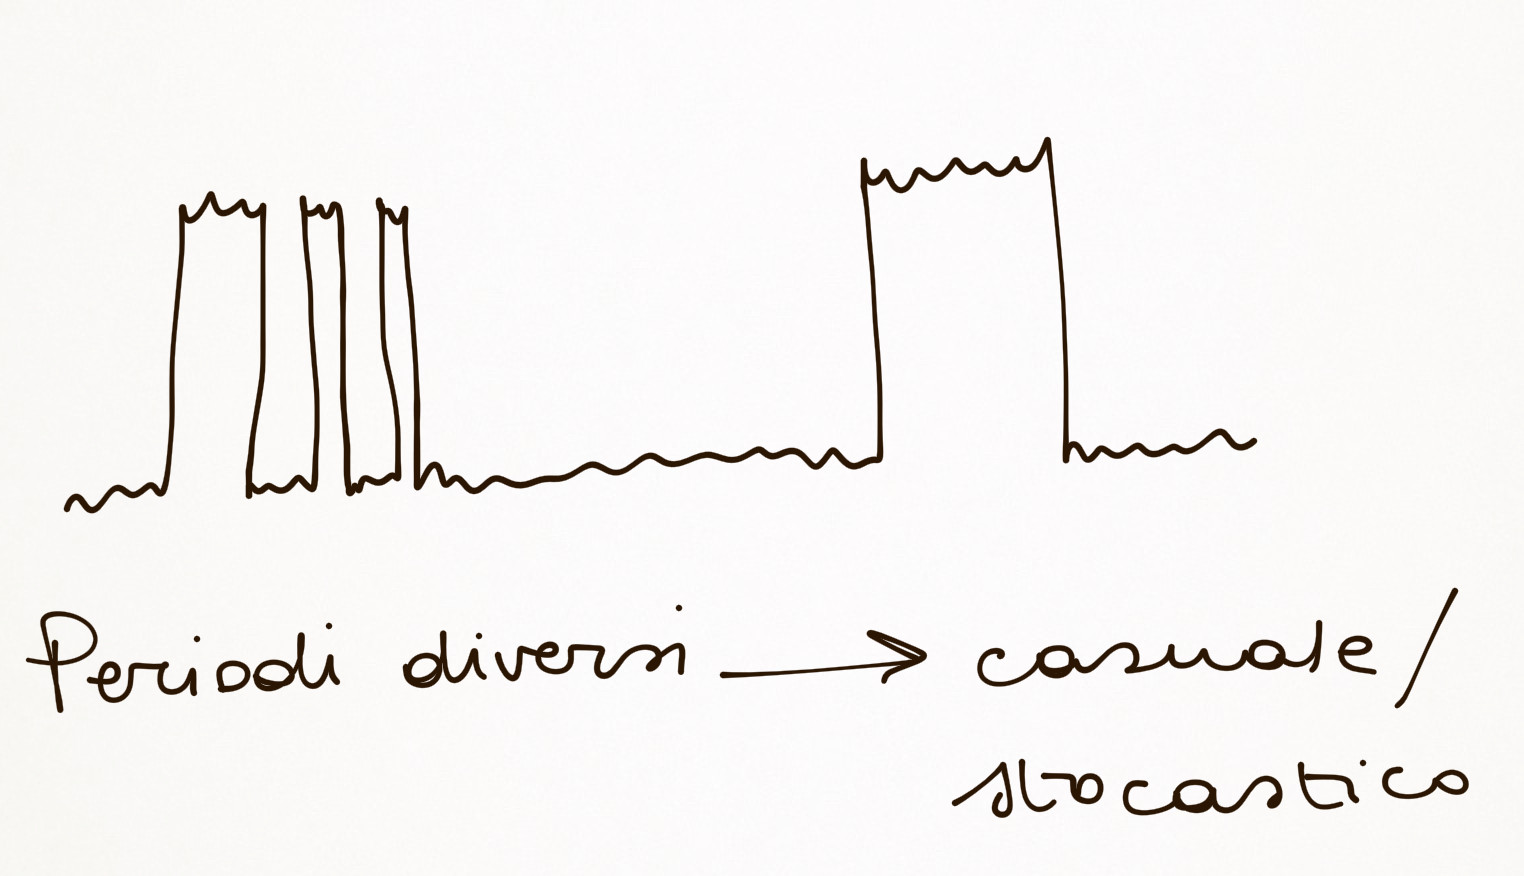
\includegraphics[scale=0.1]{immagine/4.jpg}
\caption{...}
\end{figure}

Il livello della corrente a canale aperto è una costante.

\paragraph{}
Per capire la valenza funzionale dei parametri rilevanti nell'attività di un canale: la traccia con rumore minore (a canale chiuso) è dovuta al fatto che una piccolissima parte di corrente scappa attraverso il sigillo (\emph{corrente di perdita}). Questa corrente è costante. 
\begin{figure}[H]
\centering
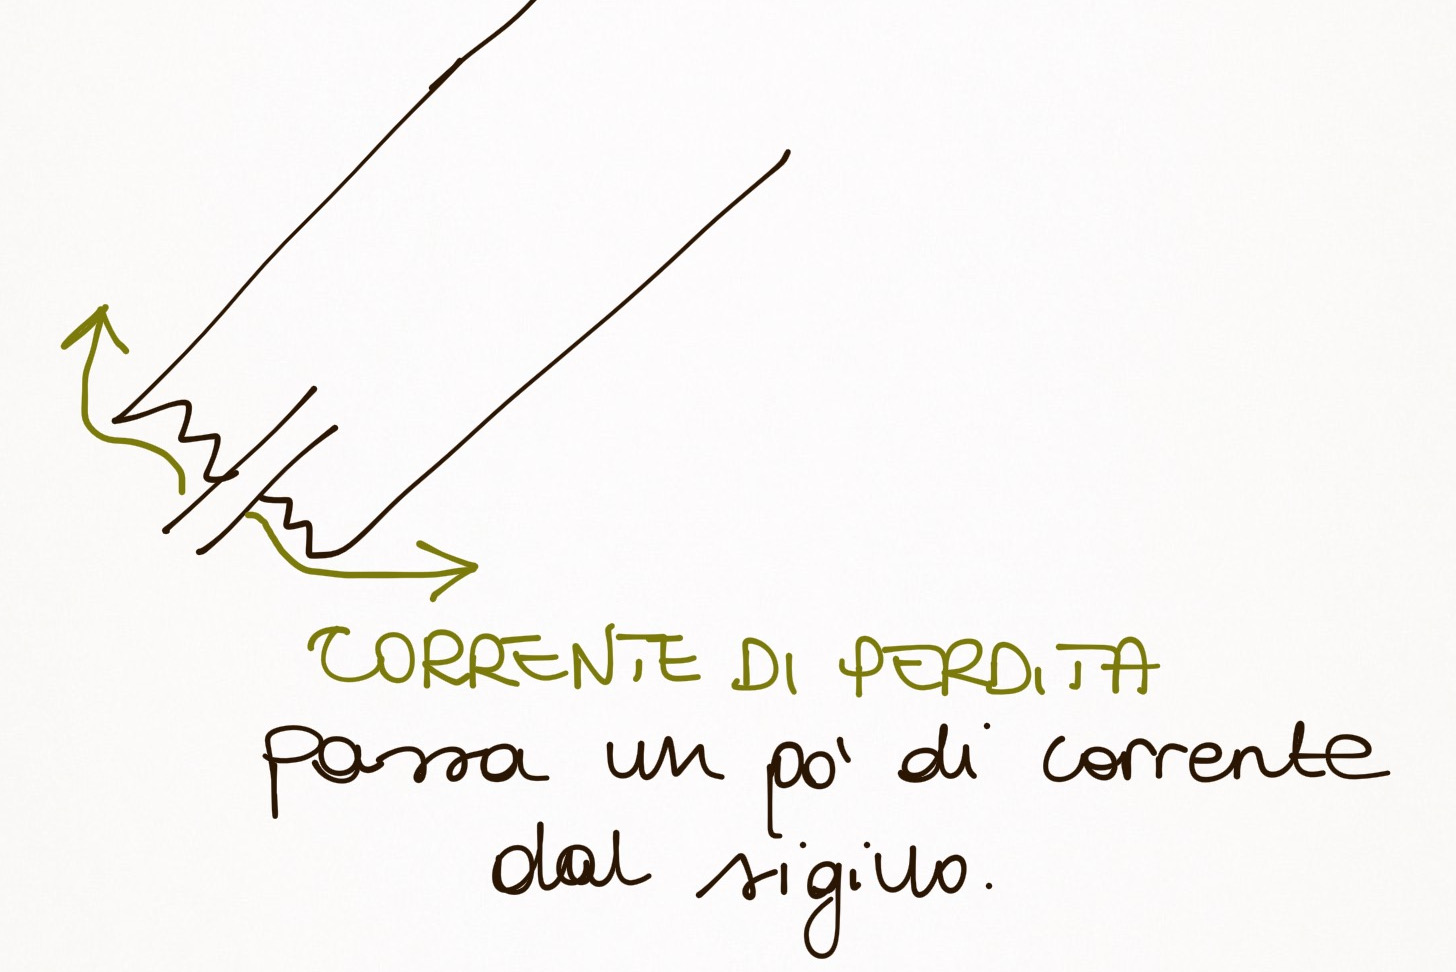
\includegraphics[scale=0.1]{immagine/5.jpg}
\caption{Corrente di perdita}
\end{figure}

Il livello di corrente più basso è dato dalla corrente a canale chiuso, ed è diverso da 0 (corrente di perdita).

Il livello alto è la somma della corrente passiva di perdita e della corrente di canale:

\begin{figure}[H]
\centering
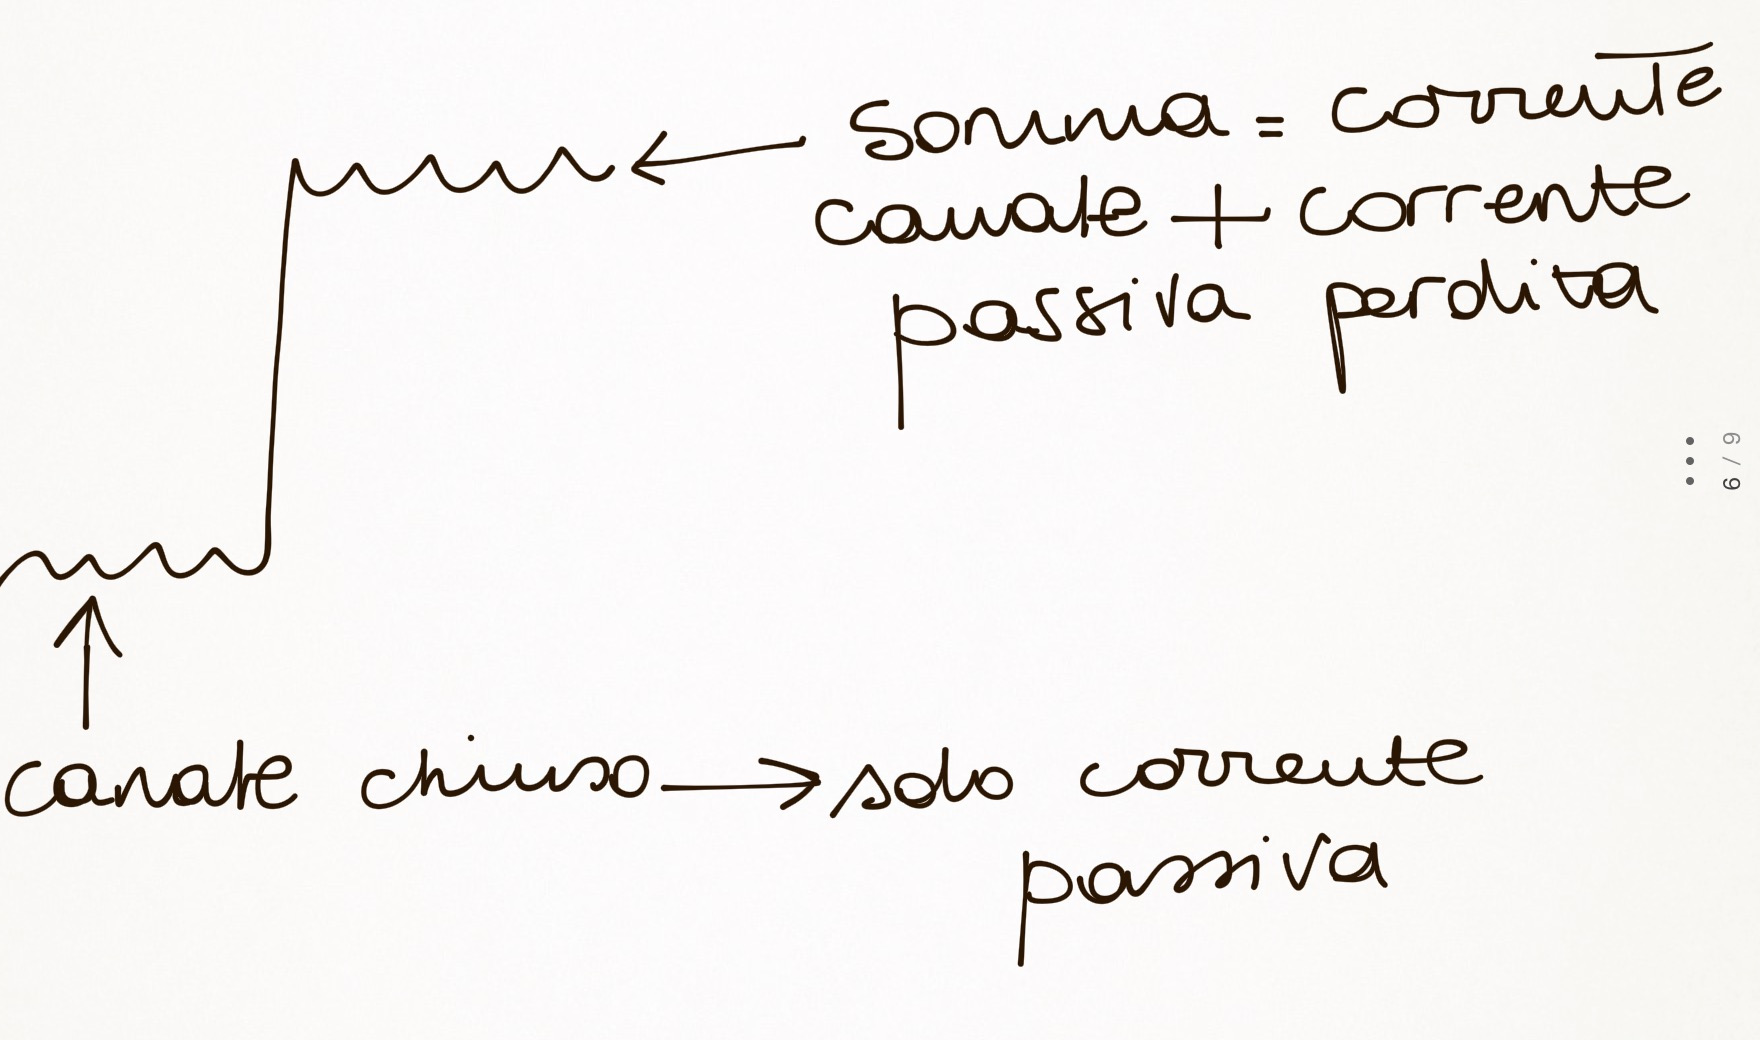
\includegraphics[scale=0.1]{immagine/6.jpg}
\caption{Livelli di corrente}
\end{figure}

La transizione verso l'alto (freccia gialla) corrisponde alla transizione chiuso \freccia aperto. La freccia rossa è il processo opposto:

\begin{figure}[H]
\centering
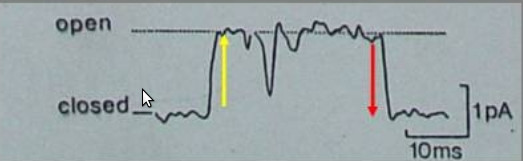
\includegraphics[scale=0.40]{immagine/can.jpg}
\caption{Schema di passaggio da canale chiuso a canale aperto (freccia gialla) e da canale aperto a chiuso (freccia rossa)}
\end{figure}


\paragraph{Come si comporta la registrazione se immettiamo uno stimolo?}

Segnale registrato da canali K degli eritrociti umani: sono a \emph{controllo chimico}, vedono il $Ca^{2+}$ sul versante intracellulare ed tanto più la concentraizone è alta, tanto più i canali sono attivi (vedi slides con Ca 0,1 $\mu M$ e 10 $\mu M$).

A concentrazione più alta, abbiamo un maggior numero di transizioni chiuso/aperto. La durata media delle aperture è cresciuta: il canale si apre più spesso e mediamente per un tempo maggiore. A parità di temperatura, le transizioni sono più facili rispetto al caso in cui si ha una concentrazione più bassa di Ca. Lo stimolo \emph{aumenta la probabilità che il canale, sotto la sollecitazione dell'agitazione termica, si apra}.

Se si hanno \emph{3 canali} nel tassello, il segnale è multilivello e abbiamo 4 livelli di corrente:
\begin{itemize}
\item{Chiuso}
\item{Aperto 1}
\item{Aperto 2}
\item{aperto 3}
\end{itemize}

La velocità di transizione ci permette di vedere quando si passa da 1 canale aperto a 2 aperti a 3 aperti.

\subsubsection{Come analizziamo i segnali?}

\begin{figure}[H]
 \centering
 \subfloat[]%[\emph{Gel 1 con frazioni 28, 29, 30}.]
{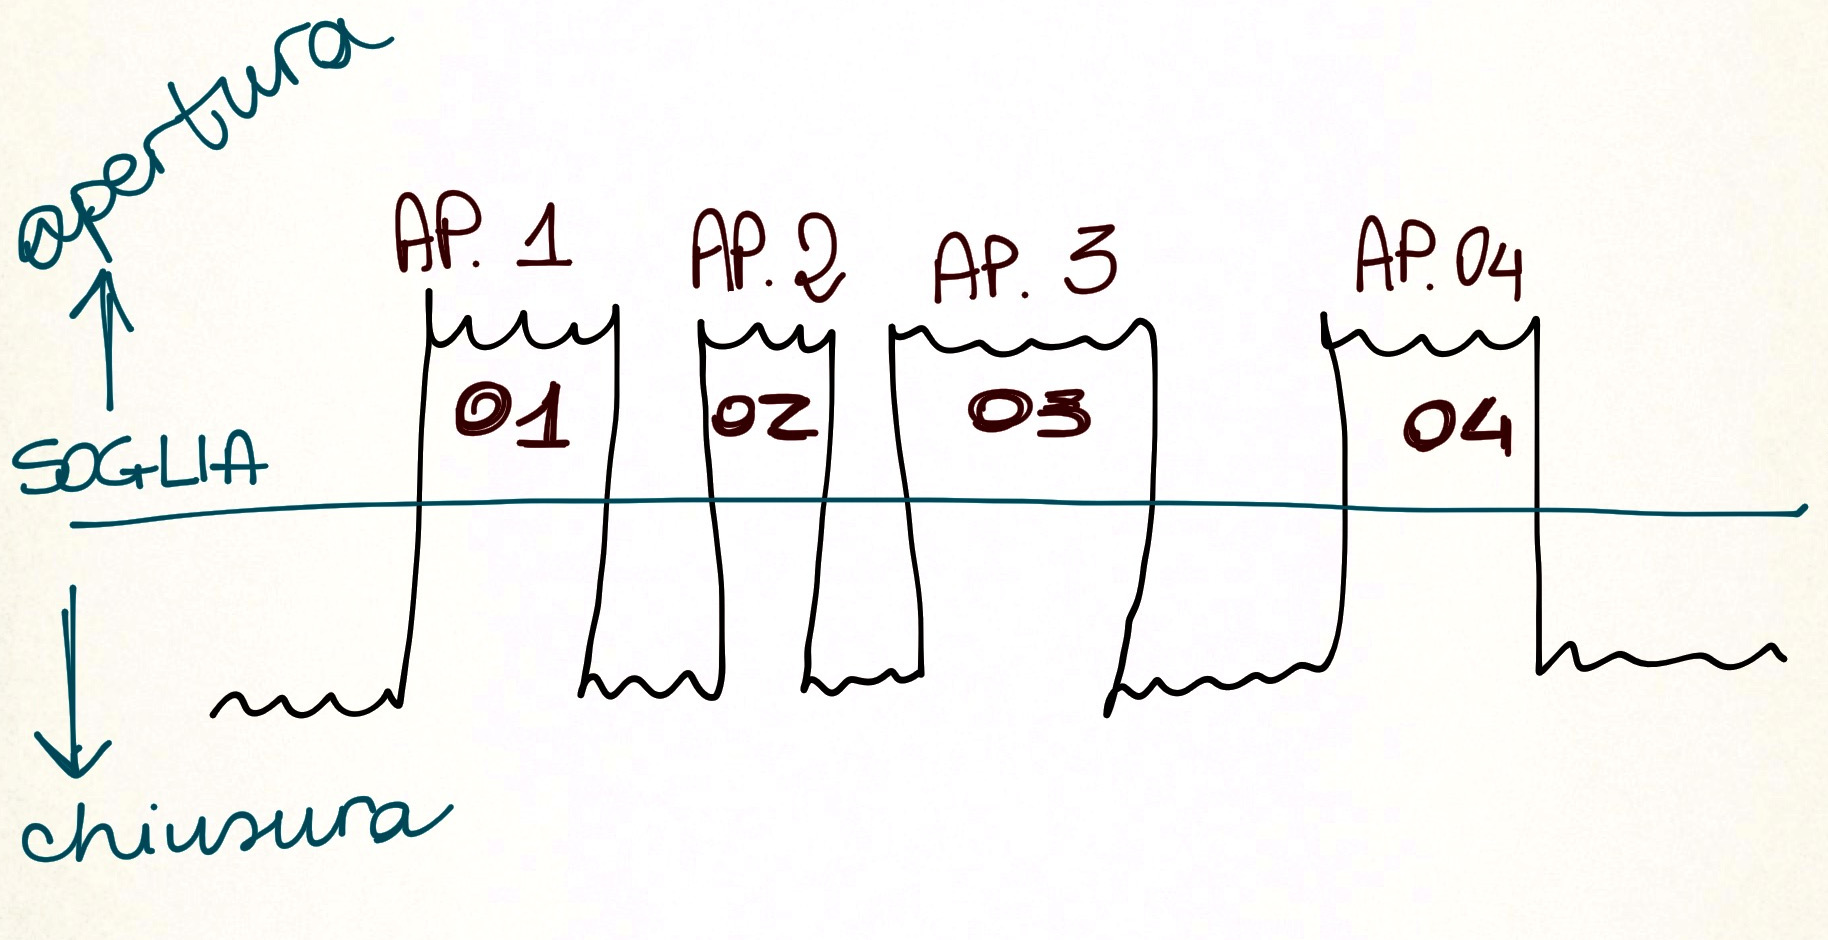
\includegraphics[width=.43\textwidth]{immagine/8.jpg}}
\label{img:a} \quad
\subfloat[]%[\emph{Gel 2 con frazioni 31, 32, 33 e 34}.]
{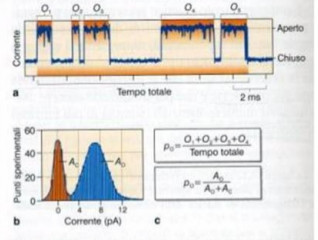
\includegraphics[width=.45\textwidth]{immagine/azzurro.jpg}}
    %\caption{Elettroforesi SDS-PAGE per le $\alpha$-cristalline}
\end{figure}

Il tracciato in azzurro è il livello di corrente a \emph{canale aperto}. Se mettiamo una soglia a metà ampiezza e si considera ciò che è sopra soglia una apertura e ciò che è sotto soglia una chiusura, possiamo misurare quanto tempo  il canale sta aperto sul tempo totale \lfreccia calcoliamo la \emph{probabilità di apertura del canale} (figura b).

Il segnale viene campionato: disponendo i punti che registra il calcolatore nell'istogramma \emph{all points}, troviamo i punti su vari livelli. 
\begin{figure}[H]
\centering
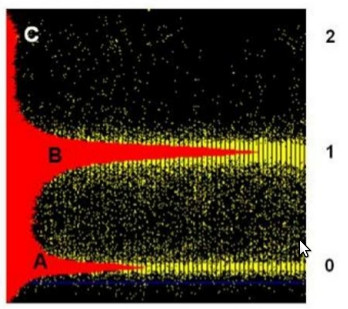
\includegraphics[scale=0.4]{immagine/all.jpg}
\caption{Istogramma all points.}
\end{figure}
Abbiamo una serie di punti sul livello 0 e 1 e qualche punto sul livello 2. Se vediamo la densità di punti in un livello di corrente, il numero di punti che assumono quel valore di corrente li rappresentiamo con un picco rosso: è una \emph{distribuzione di frequenza}. I picchi corrispondono alla \emph{densità} dei punti. Possiamo rappresentare il segnale come una doppia distribuzione gaussiana (vedi immagine precedente): la marrone è il livello chiusura.

calcolando l'integrale di ogni area, troviamo la probabilità di apertura.

La dispersione di rumore è maggiore in apertura come notiamo in figura. Per calcolare la probabilità di apertura possiamo anche fare l'integrale sotto le due curve.

Via via che il segnale scorre, vediamo in $pA$\footnote{pico ampère} l'istogramma:

\begin{figure}[H]
\centering
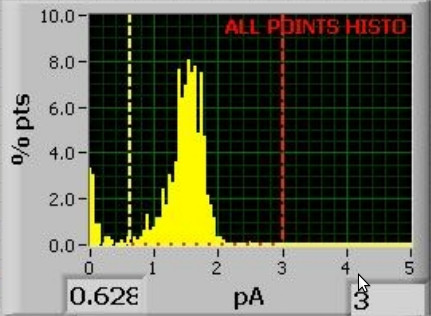
\includegraphics[scale=0.4]{immagine/giallo.jpg}
\caption{Istogramma all points rovesciato}
\end{figure}

Sapendo il valore di ampiezza in pico ampère e $V_{m}$ - $E_{i}$, possiamo calcolare la conduttanza $\gamma_{i}$ del canale: nell'eritrocita è 12 pS (picoSiemens), nel cuore 10 pS:

Possiamo anche calcolare la frequenza di apertura, la probabilità, il tempo medio in cui rimane aperto/chiuso e la corrente media (integrale della somma del tempo in cui è aperto). 

I primi 4 pannelli in basso a destra (quelli colorati) mi indicano la \emph{struttura della corrente} che sto studiando:
\begin{figure}[H]
\centering
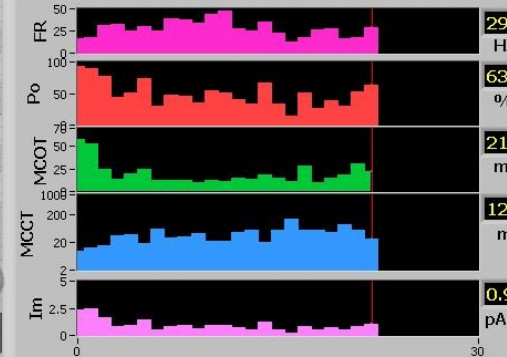
\includegraphics[scale=0.4]{immagine/color.jpg}
\caption{Struttura della corrente}
\end{figure} 
Quello più in basso è la \emph{corrente media}, misurata facendo l'integrale della traccia gialla in alto a sx. Monitorando continuamente l'integrale e sapendo il valore dell'ampiezza, ricaviamo un contributo alla conduttanza del tassello. Il primo in alto invece è la frequenza di transizioni e cambia se cambia la temperatura.
Il secondo dà la probabilità di apertura; il terzo il tempo medio aperto e il quarto il tempo medio chiuso.

Consideriamo un canale che mediamente si apre così:
\begin{figure}[H]
\centering
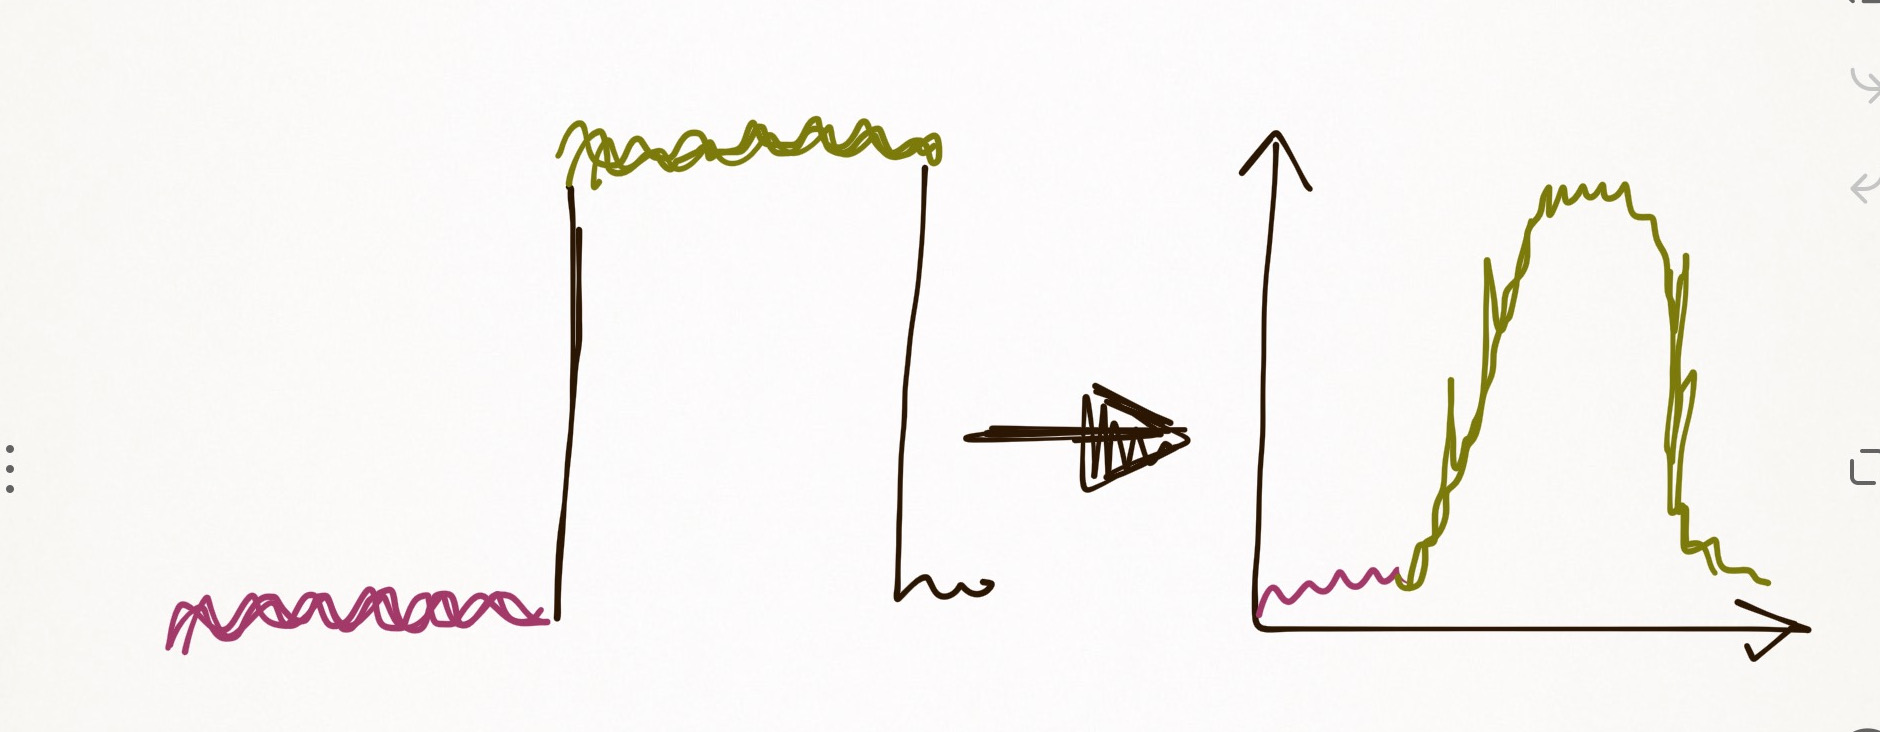
\includegraphics[scale=0.1]{immagine/9.jpg}
\caption{...}
\end{figure} 

Immaginiamo ora di registrarla in presenza di un agente bloccante, che entra nel canale, resta lì per un po' e poi viene staccato dall'agitatore termico. L'apertura con tratto marcato è il risultato dell'ingombro dell'agente bloccante.

\begin{figure}[H]
\centering
\includegraphics[scale=0.1]{immagine/10.jpg}
\caption{...}
\end{figure} 

Alcuni bloccanti realizzano una saturazione temporanea del canale e ne riconosciamo l'attività andando a guardare la struttura della corrente e la probabilità di apertura.
Se correliamo ciò con la frequenza di apertura e con il tempo medio aperto/chiuso, la struttura appare in tutta la sua chiarezza. Ciò si applica nel campo di farmacologia molecolare. Queste molecole entrano ed impegnano per un certo tempo il canale, altri farmaci cambiano completamente il quandro della conduttanza, perchè disturbano continuativamente il passaggio di ioni.

Gli istogrammi in basso a sinistra invece hanno a che fare con le \emph{proprietà cinetiche} : sono le distribuzioni degli intervalli aperti (a sinistra) e chiusi (a destra). Deduciamo i cambi di conformazione da una sola misura, non da una media di misure. 

Nel caso in cui avessimo due canali, avremmo segnali a 3 livelli. I canali si aprono e chiudono indipendentemente gli uni dagli altri o c'è cooperazione tra loro? 

Si guarda allora la \emph{statistica di Poisson}: misuro il tempo totale ai vari livelli, anche al chiuso. Avrò istogrammi fatti così:

\begin{figure}[H]
\centering
\includegraphics[scale=0.4]{immagine/picchi.jpg}
\caption{Apertura e chiusura dei canali}
\end{figure}

Li confronto con la distribuzione di poisson così definita: ammettendo una probabilità individuale che il canale cambi conformazione, ho questa formula:
\begin{equation}
\centering
P(r)={\frac{n!}{(n-r)!}} p^{r} (1-p)^{n-r} 100
\end{equation}
dove n è il numero totale di canali ed r è il numero di canali aperti.

I livelli sperimentali e teorici sono vicinissimi \lfreccia dimostriamo che \emph{un canale si apre e si chiude indipendentemente da un altro}.

\paragraph{Come si fa l'analisi cinetica e cosa vuol dire studiare la cinetica del canale?}
Mettiamo una soglia (linea gialla tratteggiata) a metà dell'ampiezza di apertura, poi conversione del segnale in segnale \emph{dializzato}, ovvero eliminando il rumore, poi si fa un istogramma di frequenza per gli intervalli aperti e chiusi. 

\begin{figure}[H]
\centering
\includegraphics[scale=0.4]{immagine/cinetica.jpg}
\caption{}
\end{figure} 
Otteniamo due istogrammi che hanno la forma di \emph{esponenziale negativo}, dove in ascissa abbiamo le classi di durata delle apertura e in ordinata il numero di aperture: consideriamo un canale allo stato chiuso che passa ad uno stato apertp con una la \emph{probabilità di transizione} $\alpha$: la probabilità di transizione però è anche funzione del tempo:
\begin{equation}
\centering
P_{CO}= \alpha t
\end{equation}
Inizio a contare quando il canale si apre e vedo quanto tempo serve prima che si chiude. Più $\alpha$ è grande, maggiore sarà la probabilità che si passi da chiuso ad aperto e vice versa.

\begin{figure}[H]
\centering
\includegraphics[scale=0.1]{immagine/12.jpg}
\caption{Rappresentazione grafica dell'equazione sopra citata.}
\end{figure} 
Questa probabilità cresce con il tempo. $\alpha$ è la pendenza della retta.

Troviamo moltissimi intervalli brevi e sempre meno intervalli più  lunghi. Dato che tutte queste distribuzioni sono esponenziali, possiamo interpolarle con una certa funzione, \emph{pdf} (funzione di densità di probabilità); ogni interpolazione sarà la linea che passa nel centro delle colonnine dell'istogramma:

\begin{equation}
\centering
pdf= Ae^{\frac{-t}{\tau_{1}}} + Be^{\frac{-t}{\tau_{2}}} \ldots 
\end{equation}

Si tiene conto di quanto velocemente cade l'esponenziale; possiamo avere due possibilità\todo{allega immagine di shut e open}:
\begin{enumerate}
\item{L'esponenziale descrive perfettamente l'andamento}
\item{La prima interpolazione è diversa dalla seconda}
\end{enumerate}

Si può calcolare con procedure di fitting.

Per riconoscere un certo tipo di canale è importante conoscere il $\tau$, la \emph{costante di decadimento}: ogni canale infatti ha una $\tau$ caratteristica. 

Se abbiamo \emph{2 esponenziali} (nel caso di shut) nei canali chiusi? Anzichè avere una sola configurazione chiusa ed una sola aperta, il canale ha \emph{2 configurazioni chiuse}, $C_{2}$ e $C_{1}$. Ogni volta che il canale si chiude potrà o riaprisi o andare in $C_{2}$, e poi per aprirsi dovrà fare un certo numero di transizioni.

Ciò è importante per l'azione degli stimoli che dei bloccanti. Se stimoliamo, le costanti di probabilità cambiano e favoriscono una conformazione $C_{2}$ o $C_{1}$. Agendo con un farmaco, vediamo qual è la conformazione più suscettibile.

(18.02.2015)
\subsection{Studiare il fenomeno di rettificazione}
Proprietà dei circuiti che consiste nel  far passare  meglio il flusso di ioni in una direzione rispetto alla direzione opposta.

Mettiamoci in questa condizione: pipetta patch, canale selettivo al potassio, inside-out. Mettiamo KCl 120 mM nella pipetta e anche all'esterno \lfreccia soluzioni simmetriche.
\begin{figure}[H]
\centering
\includegraphics[scale=0.1]{immagine/14.jpg}
\caption{Condizioni sperimentali.}
\end{figure} 

La corrente di K sarà data dalla solita fomula i = $\gamma (V_{m}-E_{k})$, ma $E_{k}= \frac{RT}{}t$, il termine del logaritmo diventa 1 ed Ek diventa 0, quindi possiamo indurre una corrente proporzionale al Vm ed avere una relazione lineare (se non c'è retificazione).

Se costruiamo un grafico misurando i e variando $V_{m}$, a $V_{m}$=0 abbiamo i=0. Man a mano che $V_{m}$ diventa più depolarizzante, avremo una retta (perchè è una relazione lineare) \lfreccia $\gamma$ è una costante.

Se il canale rettificasse, avremmo dei punti che divergono dai valori lineari: 

\begin{figure}[H]
\centering
\includegraphics[scale=0.1]{immagine/15.jpg}
\caption{Confronto tra andamento lineare e fenomeno di rettificazione}
\label{img:rett}
\end{figure} 

Il fatto che variando $V_{m}$ varia i, non significa che il nostro è un canale voltaggio dipendente. La elazione per cui i varia con $V_{m}$ è data dalla legge di Ohm. Se il canale fosse voltaggio dipendente, varierebbe anche il tempo totale in cui troviamo aperto il canale \lfreccia \emph{aumenta la probabilità di apertura}.

\begin{figure}[H]
\centering
\includegraphics[scale=0.4]{immagine/lineare.jpg}
\caption{Diagramma corrente-voltaggio e segnale ai vari $V_{m}$}
\end{figure}
 
Sul plot, la linea tratteggiata rossa è il comportamento atteso per un comportamento lineare; la deviazione nel terzo quadrante indica la presenza di rettificazione.
Il canale è quindi rettificante e passivo: se confrontiamo lo schema delle correnti a +80 mV e a - 80mV, se fosse non rettificante dovremmo avere la stessa ampiezza, ma le ampiezze sono diverse, quindi è \emph{rettificante}.
Diciamo che è \emph{passivo (voltaggio indipendente)} perchè a +80 mV il canale è aperto all'80 \% (di tempo). A -80 mV la corrente inverte (cambio segno), ma si ha comunque l'80 \% di tempo in cui il canale è chiuso.

\subsubsection{Calcolo del valore di conduttanza}
\begin{equation}
\centering
\gamma_{K}= \frac{i_{k}}{V_{m}}
\end{equation}

Prendiamo un canale \emph{voltaggio dipendente non rettificante}: abbiamo 2 canali, nel pannello B in alto (+60 mV) entrambe i canali hanno alta probabilità di apertura, perchè entrambe i livelli sono attivati spesso. A + 40 il secondo livello è meno attivo, a +20 mV scompare il secondo livello: i due canali non sono mai aperti insieme. A -80 c'è un solo canale aperto una volta: questo canale \emph{modula la probabilità di apertura in funzione del voltaggio}.

\begin{figure}[H]
\centering
\includegraphics[scale=0.4]{immagine/nonret.jpg}
\caption{Canale voltaggio dipendente non rettificante}
\end{figure} 
La probabilità di apertura diminuisce con l'iperpolarizzazione ed aumenta con la depolarizzazione. I canali \emph{funny} invece si comportano in modo opposto.

Prendiamo un canale \emph{meccanicamente attivato}: o si isola come \emph{inside-out} e poi si applca una piccola pressione all'interno della pipetta (in alto a sx)e, facendo una pressione di pochi mmHg all'interno della pipetta, la membrana viene distesa ed il canale si attiva. Se portiamo la pressione a -80 mmHg, abbiamo la massiccia attivazione dei due canali; a -40 mmHg la probabilità di apertura è minore.

Oppure in \emph{cell-attached}, mettendo una soluzione ipotonica che fa un eccesso di acqua esterno, l'acqua tende ad entrare nella cellula e a distendere la membrana.

L'ampiezza della corrente quindi dipende dal voltaggio che mettiamo, ma quella che varia è la probabilità di apertura.

Quando dobbiamo cambiare soluzione all'esterno, usiamo la \emph{microperfusione} e ci mettiamo in inside-out:

\begin{figure}[H]
\centering
\includegraphics[scale=0.4]{immagine/microperfusione.jpg}
\caption{Schema della microperfusione}
\end{figure} 

I capillari di vetro sono percorsi da soluzioni a diversa conduzione, che scegliamo noi: questo dispositivo cambia rapidamente posizione e così cambia rapidamente (2 ms) quale soluzione bagna il tassello (in viola) che si trova nella pipetta. La corrente di soluzione che ogni capillare genera è incontaminata. 

Volendo studiare la sensibilità al Ca della faccia itracellulare, abbiamo un tassello in inside out e facciamo passare soluzioni diverse in termini di concentrazione libera di Ca: mescoliamo i sali di Ca con dei chelanti e con un buffer stabiliamo la pK della soluzione. Possiamo fare la stessa cosa con un tassello outside out, ma per un neurotrasmettitore.

\subsubsection{Selettività del canale}

Per studiare la selettività, prendiamo un canale rettificante passivo e vediamo a cosa è selettivo: registriamo all'inizio con soluzioni di KCl 120 mM all'interno della pipetta e all'esterno. Per vedere se il canale è selettivo al Cl o al K, presentiamo KCl 60 mM all'esterno: non siamo più nella condizione precedente, ma abbiamo una $E_{K}$ o $E_{Cl}$ diverse da 0 perche $E_{K} =$\todo{cerca la formula!!!}.

$E_{K}$ passa da 0 a +17.5 mV. La forza elettromotrice dipende ora da $V_{m}$-$E_{K}$, che è diverso da 0. Se il canale segue l'equazione di Nernst per il K, è selettivo per il K. Sul grafico, dove si annulla la corrente? a +17.5 mV.
\begin{figure}[H]
\centering
\includegraphics[scale=0.4]{immagine/selettivita.jpg}
\caption{Studio della selettività per K e per Cl}
\end{figure} 

Perchè si dice che è selettivo per il K e non per il Cl? Perchè se calcoliamo $E_{Cl}$, e se il canale fosse selettivo per Cl, il valore che vediamo sul grafico, in cui si annulla la corrente, dovrebbe essere -17.5 mV.

E se fosse un canale cationico? Se andasse bene un altro ione monovalente?

Se sostituiamo il K con l'equivalente Na:
\begin{itemize}
\item{O il nuovo catione passa e la corrente di K è trascurabile}
\item{O Na viene filtrato e passa solo K}
\end{itemize}

Se il Na passa, deve essere una corrente misurabile. È quello che vediamo nel diagramma in basso: nei voltaggi positivi, l'esterno è positivo rispetto all'interno della pipetta.

Questo è quindi un canale \emph{cationico altamente selettivo allo ione K}.

\subsection{Canali voltaggio-dipendenti chimicamente-sensibili}
Hanno due tipi di sensori: di voltaggio e chimico. Ad esempio, il sensore per il Ca è situato nella faccia intracellulare. La permeabilità di membrana al K, ovvero quanto la membrana riesce a spostare il sui potenziale di equilibrio verso quello del potassio, è accoppiata all'attività metabolica della cellula, in particolare alla quantità di Ca ionico libero cellulare. Il Ca è un \emph{messaggero intracellulare}.

Canali di questo tipo correlano l'attività elettrica di cellule eccitabili alla situazione specifica di questo messaggero intracellulare. Possiamo studiare questo canale misurando la probabilità di apertura in funzione del voltaggio, otteniamo delle \emph{sigmoidi}.
\begin{figure}[H]
\centering
\includegraphics[scale=0.4]{immagine/sigmoidi.jpg}
\caption{Probabilità di apertura in funzione della concentrazione di Ca}
\end{figure} 

Diminuendo la concentrazione di Ca fino a 0,1 $\mu M$, ottengo una sigmoide slittata sull'asse X e i canali hanno una maggior probabilità di apertura a potenziali più positivi rispetto all'avere una concentrazione di 10 $\mu M$. Supponendo di metteric a +20 mV, con Ca basso la probabilità di apertura è minore rispetto ad una situazione in cui la concentrazione di Ca è più elevata. Il canale ha quindi i due sensori già anticipati.

(23.02.2015)

\section{Correlazioni correnti microscopiche e macroscopiche}
Che rapporto c'è tra un evento legato alla statistica (apertura o meno dei canali ionici) e il profilo temporale delle correnti macroscopiche\footnote{Attraverso l'intera membrana, tramite la tecnica patch clamp. La corrente microscopica è quella che osserviamo attraverso un solo canale}?

In voltage clamp, isolavamo una \emph{corrente di capacità}, che parte da 0, rapidamente si istaura ad un certo valore, poi decade esponenzialmente a 0, e una \emph{corrente di perdita}, che si fa fluire attraverso i cnali passivi e serve per mantenere il voltaggio di comando per un certo tempo ($I_{L}$, corrente di lineage o passiva). Poi una \emph{corrente entrante }con andamento transitorio ($I_{Na}$): pur mantenendo lo stimolo, la corrente si estingue piano piano \lfreccia inattivazione. Poi una corrente potassio ($I_{K}$) che si sviluppa con minore velocità, ma poi permane per tutto il tempo che la depolarizzazione permane. 

\begin{figure}[H]
\centering
\includegraphics[scale=0.1]{immagine/16.jpg}
\caption{Tipi di corrente studiati sinora}
\label{img:corrente}
\end{figure} 

Mentre la corrente Na va incontro ad inattivazione, questa corrente K no.

\emph{Come raccodriamo queste immagini che denotano la corrente che passa \emph{in parallelo} attraverso diversi canali, con i segnali che registriamo da un singolo canale?}

Nel caso dei singoli canali il comportamento è stocastico: solo la probabilità di questo evento stocastico può essere aumentata o diminuita; per le correnti macroscopiche invece il fenomeno è un evento discreto. Eseguendo stimolazioni tutte uguali, otteniamo risposte identiche, con forse l'unica differenza del rumore. 

Come possiamo partire da un singolo canale ed ottenere qualcosa che somiglia alla figura \ref{img:corrente}?

Trasponiamo il fenomeno \emph{dal tempo allo spazio}: 
\begin{figure}[H]
\centering
\includegraphics[scale=0.1]{immagine/17.jpg}
\caption{Voltage clamp con un solo canale}
%\label{img:corrente}
\end{figure} 

Stimoliamo con un certo V di comando e registriamo le correnti in entrata ed uscita che passano attraverso molti canali \lfreccia con un solo stimolo temporale attiviamo molti canali spazialmente distribuiti sulla membrana. Come posso mimare questo, ma lavorando su \emph{un singolo canale?}, quindi con la tecnica del patch-clamp.

Se assumo che la membrana contenga n canali, se registro da un singolo canale e ripropongo lo stesso potenziale di comando, avrò il segnale elementare che passa attraverso un singolo canale.

Se \emph{stimolo un singolo canale n volte}, devo avere la stessa cosa che ho ottenuto stimolando una sola volta gli n canali\footnote{supponendo che le proprietà di canali dello stesso tipo siano uguali}.

\subsection{Canale K passivo}
Posso scegliere in una membrana eccitabile che abbia canali passivi per il K, attivi per il Na, voltaggio dipendenti per il K o per il Na, e fare ciò.

In riferimento alla figura \ref{img:rett}, facendo il rapporto tra corrente e voltaggio nella parte lineare, la conduttanza era circa 100 pS.

Sottoponiamo un tassello con un solo canale ad una depolarizzazione da 0 a +50 mV\footnote{Stiamo lavorando in una condizione in cui la concentrazione all'esterno e all'interno della pipetta è 120 mM di K, ottima per cimentare i canali selettivi al K}:
\begin{itemize}
\item{Se stimolo la prima volta e registro da un canale singolo, a 0 non vedrò nulla e a +50 mV vedrò apertura} 
\item{Se stimolo una seconda volta, l'andamento stocastico sarà diverso dalla prima stimolazione e così via}
\end{itemize}
Stimolando le varie volte, le tracce hanno di simile che, sommando il tempo in cui il canale è allo stato aperto, e mettendolo in relazione con il tempo totale analizzato, è circa l' 85 \% (il tempo che rimane aperto). Siccome le correnti sono in parallelo, faccio una somma di tutti i segnali punto per punto: ottengo il profilo di corrente sotto la linea tratteggiata rossa:

\begin{figure}[H]
\centering
\includegraphics[scale=0.4]{immagine/tempo_d.jpg}
\caption{Apertura e chiusura dei canali in dipendenza dal tempo in condizioni di \emph{depolarizzazione}}
\label{img:a}
\end{figure} 

Perchè?

Perchè poggio e buca fa pari. Se un punto è basso, viene compensato da un punto in alto e così via. Quanto maggiore è il numero di stimolazioni, tanto più sarà regolare questo profilo. Tuttavia, questo profilo è quello che noi abbiamo disegnato nella figura \ref{img:corrente} come corrente di perdita, ovvero il comportamento nel tempo di un canale passivo: un canale passivo non ha un comportamento tempo dipendente, perchè non si attiva e inattiva come fanno i voltaggio dipendenti.

Se invece \emph{iperpolarizzo}, avrò correnti più piccole perchè \emph{il canale rettifica}. 
\begin{figure}[H]
\centering
\includegraphics[scale=0.4]{immagine/tempo_db.jpg}
\caption{Apertura e chiusura dei canali in dipendenza dal tempo in condizioni di \emph{iperpolarizzazione}}
\label{img:b}
\end{figure} 

Se prendo le ampiezze delle correnti nelle figure \ref{img:a} e \ref{img:b} e mi chiedessi quale sarebbe l'ampiezza se non ci fosse nessuna chiusura, il livello sarebbe la linea tratteggiata  rossa (100 \% di apertura).

Se vado a vedere la differenza tra l'ampiezza media misurata e quella se fosse sempre aperto, kmisuro un 85 \% in media di differenza.

Supponendo che questi canali si trovino nella stessa cellula, prendiamo cellule intere e misuriamo la \emph{resistenza di ingresso}\footnote{la resistenza che la membrana opponeva al passaggio di corrente} (vedi current clamp). La resistenza $R$ in ingresso era 50 $M \Omega$. Se esprimiamo questo dato in conduttanza (1/R), abbiamo 20 $nS$: questa membrana, per esprimere 20 nS, quanti canali di 100 pS\footnote{perchè ogni canale ha questa conduttanza} deve avere?

Devono essere \emph{200 canali} di questo tipo per giustificare una corrente di 20 nS di conduttanza. Abbiamo un certo numero n di canali per K che hanno una conduttanza $\gamma_{k}$ di 100 pS. Conoscendo la corrente elementare e la probabilità di apertura e il numero di canali, il loro prodotto ci dà la corrente totale:
\begin{equation}
\centering
I=i N P_{o}
\end{equation}

Se i canali fossero aperti al 100 \% del tempo, basterebbero i 200 canali. Visto che però abbiamo appurato che sono aperti al 85 \% del tempo\footnote{È un dato sperimentale}, i canali dovranno essere 230.

\subsection{Canale K o Na voltaggio dipendenti}
Facciamo la stessa cosa appena fatta per i canali passivi, ma per i \emph{canali voltaggio dipendenti}.

Ripetiamo la stimolazione con il potenziale di comando: abbiamo risposte diverse, ma con caratteristiche comuni. Se manteniamo il comando, tutte le risposte statisticamente stanno nella parte inizale dello stimolo, mentre nel resto non si vedono canali aperti. Se sommiamo, vediamo un andamento identico al profilo della corrente macroscopia Na dipendente in figura \ref{img:corrente}.

\begin{figure}[H]
\centering
\includegraphics[scale=0.4]{immagine/voltaggio.jpg}
\caption{Canali Na e K voltaggio-dipendenti}
%\label{img:volt}
\end{figure} 

Se facciamo la stessa cosa con il canale K, ci sono varie lacune di attività: la corrente risultante è molto simile alla corrente macroscopica di K in figura \ref{img:corrente} in cui vediamo un lento raggiungimento del tempo al picco. Una volta raggiunta l'attivazione viene mantenuta.

Mediamente, la prima latenza a cui il canale rispone è molto minore rispetto al canale Na, che ha un tempo al picco molto rapido.

Possiamo dire che la corrente macroscopica di Na si può anche esprimere come \emph{una curva di probabilità di apertura} dei canali: alto valore = alta probabilità che sia aperta. Gli stimoli quindi \emph{variano la probabilità di apertura} piuttosto che aprire i canali ionici.

Se registriamo l'attività di un \emph{canale Na cardiaco} (quello di prima era neuronale): 

\begin{figure}[H]
\centering
\includegraphics[scale=0.4]{immagine/na_cuore.jpg}
\caption{Probabilità di apertura di canale Na cardiaco wt e mutanti per aritmia cardiaca}
%\label{img:b}
\end{figure} 

Depolarizziamo da -120 a 0 mV, otteniamo più o meno la stessa cosa di prima. Preleviamo quindi qualche canale che origina da mutanti (in Xenopus) che presentano una \emph{patologia cardiaca} (aritmia negli umani): questi canali, oltre ad essere più attivi, hanno un quadro anomalo perchè presentano aperture nella parte tardiva della depolarizzazione,e questo produce una corrente che si intattiva solo parzialmente nonostante il lungo tempo di depolarizzazione (400 ms). Questi pazienti hanno una eccitazione che permane anche quando il tessuto dovrebbe stare a riposo.

\subsection{Tecniche di biologia molecolare}
È possibile individuare dei tessuti che hanno abbondanza di un certo tipo di canali, poi legarli con tossine specifiche e possono essere isolati dalle frazioni proteiche e studiati purificandoli. Alternativamente si può isolare l'RNA specifico codificante parte o un intero canale, e poi codificare un cDNA che ci servirà per l'espressione in \emph{oociti di Xenopus}.

Infine, con \emph{mutagenesi sito-diretta} possiamo modificare fino ad un singolo aa, mirando (dai dati di purificazione) a quelle regioni strategiche per la funzione del canale. Ciò ci permette di fare un rapporto tra struttura e funzione.

\paragraph{Riassumendo \dots}
\begin{itemize}
\item{I segmenti transmembrana sono collegati da vari loop.}
\item{Per il canale Na e Ca vediamo un dominio ripetuto 4 volte, mentre nel canale K solo una volta. Strutturalmente il canale intero può essere garantito da una struttura, mentre al canale K servono 4 strutture a rosetta per garantire un singolo canale}
\item{Vedendo l'omologia di un canale Na e Ca in una specie semplice e poi confrontandolo con una più avanzata, troviamo una omologia altissima: queste strutture, da quando sono comparse evolutivamente, sono state un vantaggio così grande che si sono conservate. Un \emph{progene} ha espresso per primo questo tipo di struttura, che è stata mantenuta e complicata ulteriormente a servizio di varie selettività}
\end{itemize} 


Se estendiamo l'analisi e chiamiamo i canali ionici che chiamiamo \emph{recettori ionotropici}, e li confrontiamo con i voltaggio-dipendenti Na, vediamo che entrambi si compongono di vari domini, che si dispongono a rosetta formando il canale acquoso. Non si ha un solo polipeptide, ma 5 diversi (nei voltaggio dipendenti invece la proteina è una sola). Il canale nello stadio embrionale, quando si realizzano i contatti tra cellule nervose e muscolari, presenta delle subunità diverse.

Stessa cosa per il canale K voltaggio dipendente: deve mettere insieme dei tetrameri generati da proteine diverse. Per quale motivo alcuni canali presentano questa codifica in un solo gene ed altri sono più articolati?

I canali più conservativi sono il canale Na e Ca voltaggio dipendente, mentre più articolati sono quelli sotto controllo chimico e i canali potassio.

Il vantaggio della situazione in cui si compone il canale partendo da più peptidi è che possiamo comporre variamente diverse strutture: possono esistere in molti sottotipi, oltre a quelli generati dallo splicing alternativo ecc.

I canali K possono essere composti o da \emph{omotetrameri} o da \emph{eterotetrameri}, a loro volta molto diversi in termini di subunità. Possono esistere un numero enorme di sottotipi, visto che il canale K è composto.

Per quanto riguarda l'$\alpha$ subunità\footnote{la porzione del canale che ha le proprietà di poro acquoso e di controllo primario}. 
 
\begin{figure}[H]
\centering
\includegraphics[scale=0.4]{immagine/canalopatie.jpg}
\caption{Patologie da cattivo funzionamento dei geni che catalizzano per le subunità recettoriali}
%\label{img:b}
\end{figure} 

Il canale vero e proprio, per funzionare come tale, si complessa con altre subunità del canale voltaggio dipendente del Na, i geni differiscono a seconda delle diverse destinazioni in cui i canali devono essere impiegati. A destra vediamo le canalopatie, ovvero le patologie conosciute la cui  eziologia è legata al cattivo funzionamento del gene corrispondente.

\paragraph{Domini dei canali Na voltaggio dipendenti}
i dati sono prelevati da mutagenesi sito-diretta connessa con un'analisi elettrofisiologica patch clamp.

I canali Na hanno \emph{segmenti S4} che sono i\emph{sensori di potenziale}; poi il \emph{loop S5-S6}, responsabile della \emph{selettività}. Il link che lega il segmento S6 con la successiva struttura è responsabile della \emph{inattivazione del Na di tipo veloce}.


\begin{figure}[H]
\centering
\includegraphics[scale=0.45]{immagine/s4.jpg}
\caption{Domini dei canali Na voltaggio-dipendenti}
%\label{img:b}
\end{figure} 

Si distinguono due tipi di inattivazione:
\begin{enumerate}
\item{Una che porta a velocemente a bassi livelli di corrente dopo il picco}
\item{Una che porta a 0 più lentamente}
\end{enumerate}

Le subunità $\beta_{1}$ e $\beta_{2}$ coadiuvano alla funzione di inattivazione. Nell'immagine sottostante vediamo la disposizione dei vari domini e la sferetta indica il sito di legame della \emph{tetrorodossina}, che agisce tappando il canale e coordinano questi siti rappresentati come sfere ed ingombrando il passaggio.
\begin{figure}[H]
\centering
\includegraphics[scale=0.5]{immagine/domini.jpg}
\caption{}
%\label{img:b}
\end{figure} 

Un filtro di selettività va da 0.3 a 0.4 $nm$ e gli S4 sono i sensori di voltaggio.

\subsubsection{Clonaggio di canali e recettori}
Per purificare un canale servono delle tossine, che hanno:
\begin{itemize}
\item{Legame covalente tenace}
\item{Altissima specificità, perchè alla conservazione della struttura del canale corrisponde una specializzazione sempre maggiore dei veleni}
\end{itemize}

Molte tossine si rivolgono a canali Na voltaggio dipendenti e a canali dei neurotrasmettitori. I canali meccanocettivi sono gli ultimi ad essere stati studiati perchè non sono state specializzate molte tossine contro di essi, poichè non controllano i target delle tossine (respirazione, muscolo cardiaco).

Si può partire da RNA, separarne frazione ed iniettarle negli oociti di Xenopus, i quali esprimono i canali di membrana.

Alternativamente si fabbricano delle \emph{cellule artificiali} che possono essere dei \emph{liposomi}: se vi aggiungiamo proteine canale purificate, la superficie del liposoma diventa una sorta di membrana che può essere studiata con le tecniche di patch clamp. 

Qui vediamo la subunità $\beta$ ed il diverso profilo della corrente:
\begin{figure}[H]
\centering
\includegraphics[scale=0.4]{immagine/beta.jpg}
\caption{}
%\label{img:b}
\end{figure} 

Entrambe le correnti inattivano, ma c'è una parte di attivazione della corrente garantita dalla coespressione della subunità $\beta_{1}$ insieme alla $\alpha$. La alpha è già in grado da sola ad esprimere la funzionalità del canale, mentre la beta contibuisce ad offrire una più rapida inattivazione.

Come si è arrivati a identificare le varie funzioni di una parte del canale? Facendo \emph{sostituzioni mirate}.\subsubsection{Sostituzioni di aa}
Nel segmento S4, ogni 3 aa ce ne era uno di carica positiva (Arg, Lys): se sostituiti con aa neutri\footnote{C'è un modello matematico (Hodgkin e Axle) che esprime il comportamento della corrente Na punto per punto. Il parametro $m^{3 }$ è un coefficiente che denota il grado di voltaggio-dipendenza della corrente.}, registrando la corrente vediamo un andamento con il potenziale di tipo simil-sigmoideo. 

\begin{figure}[H]
\centering
\includegraphics[scale=0.4]{immagine/axle.jpg}
\caption{Modello Hodgkin e Axle per corrente Na in funzione del voltaggio}
%\label{img:b}
\end{figure} 

Una pendenza molto rapida significa che per piccole variazioni di voltaggio $m$ cambia molto, mentre la meno ripida indica che occorre una depolarizzaizone maggiore per portare alla stessa variazione del paramentro $m$.

C'è anche la \emph{carica di gating}:
\begin{figure}[H]
\centering
\includegraphics[scale=0.1]{immagine/18.jpg}
\caption{Corrente di gating}
%\label{img:corrente}
\end{figure} 

Avendo la corrente capacitiva, che esprime le cariche che vanno a caricare il doppio strato (o il condensatore), possiamo fare delle \emph{stimolazioni simmetriche}: se ne facciamo un gran numero si verifica che, siccome il canale sposta le sue cariche in una posizione che corrisponde al canale aperto solo con la depolarizzazione, se facciamo un gran numero di somme di questi due segnali, se fossero uguali dovremmo avere 0. Se invece nel depolarizzare muoviamo delle cariche come in sensore di voltaggio (dipolo sensibile a campo elettrico), variamo la probabilità di apertura dei canali spostando un gran numero di dipoli. Se facciamo un gran numero di stimolazioni avremo delle correnti minuscole, le \emph{correnti di gating} Z, espressione del collettivo spostamento nella membrana dei sensori di voltaggio.

\begin{figure}[H]
\centering
\includegraphics[scale=0.4]{immagine/Z.jpg}
\caption{Corrente di gating in funzione della diminuzione di cariche}
%\label{img:b}
\end{figure} 

Si può misurare questa corrente Z. Sostituendo gli aa positivi con aa neutri, avremo una riduzione della carica netta positiva, e una conseguente riduzione di Z.
\paragraph{}
Il movimento delle parti del canale che risentono del voltaggio è un fenomeno che vede lo \emph{spostamento verso l'esterno e in rotazione dei segmenti S4}.

È stato possibile descrivere questo secondo due tecniche:
\begin{enumerate}
\item{Sostituire con 2 Cys alcuni aa responsabili della regione in grigio della figura \ref{img:met}, che fanno capolino verso la faccia extracellulare. Poi si fanno legare con \emph{metantiosulfonato}: sostituendo aa fino ad una certa lunghezza, vediamo reattività positiva, mentre per i residui più interni no}
\item{FRAT: trasferimento di energia in fluorescenza.}
\end{enumerate}

\paragraph{Metantiosulfonato}

Le Cys fanno reattività con il sulfonato: vedo se la membrana sottoposta a queste mutazioni si comporta in depolarizzazione come siti attivi per il metantiosulfonato. Uso praticamente la reattività come indicatore.

\begin{figure}[H]
\centering
\includegraphics[scale=0.4]{immagine/metantio.jpg}
\caption{Tecnica del metantiosulfonato}
\label{img:met}
\end{figure} 

Sostituiscono aa in posizioni ben definite: per stabilire fino a che profondità l'aa fa capolino all'esterno, uso la reattività come indicatore e la scelta dell'aa per posizionare la Cys, così vedo quale aa sporge.

\paragraph{Frat}
Sono state costruite sonde in cui mettiamo insieme un primo fluorescente, o accettore, ed un secondo, o donatore: uno assorbe una $\lambda$ più bassa e ne emette una più alta, che eccita il secondo fluporescente, il quale emetterà ad una $\lambda$ ancora più alta : questo è il \emph{trasferimento risonante di fluorescenza}.

\begin{figure}[H]
\centering
\includegraphics[scale=0.4]{immagine/frat.jpg}
\caption{Tecnica del FRAT}
\label{img:frat}
\end{figure} 

È possibile quanto più le due parti sono vicine. Per rilevare l'esistenza del fenomeno, vedo se il secondo fluorescente emette quando lo eccito con la lunghezza d'onda del primo. Lego alcuni aa del segmento S4 con una sonda fluorescnete e metto il secondo fluorescente a livello di un aa che fronteggia questa struttura: quando questo ruota e si allontana, non avrò più frat.Oppure faccio la cosa inversa, metto la frat positiva quando la struttura ruota.

\paragraph{}
Grazie alla frat e al metantiosulfonato è stato possibile definire il meccanismo di attivazione del canale Na. Diverse parti del canale Na (in particolar ei 4 domini) sono in movimento per sentire la variazione di campo. Ciò permette un cambio conformazionale che crea la pervietà del poro acquoso, ma ciò è ancora sotto studio.

(29.02.2015)
\subsection{Approfondimenti sulle funzioni dei canali ionici}

Due livelli di complessità ulteriori dei canali:
\begin{itemize}
\item{La localizzazione del canale non è causale\footnote{Già trattato quando parlavamo dell'organizzazione sopramolecolare della membrana}: è ancorata ad un citoscheletro specifico, al quale corrisponde un'organizzazione Raft, in cui il canale è immerso in chinasi, fosfatasi, Ig proteine ecc. La funzione di un canale è \emph{contingente al contesto molecolare} in cui opera}
\item{Il canale può essere \emph{modulato} : la relazione stimolo-risposta può variare in funzione di un terzo evento}
\end{itemize}

\subsubsection{Tipi di interazione chimica per i canali chimicamente controllati}
Distinguiamo il fenomeno della \emph{trasmissione}\footnote{passaggio dell'informazione dall'elemento presinaptico all'elemento postsinaptico} dalla \emph{modulazione}\footnote{variazione di potenza nel passaggio dell'informazione trasmessa}.

La sinapsi neuromuscolare opera riguardo alla trasmissione con l'\emph{acetilcolina}, che agisce sui recettori che sono canali cationici; la modulazione agisce quando i terminali orto simpatici rilasciano \emph{noradrenalina}, la quale modifica caratteristiche della membrana pre e pos sinaptica, rendendo più efficiente ed ampia la risposta post-sinaptica: la funzione è di modulare la prestazione fisica in base al livello di eccitazione dell'ortosimpatico.

Sia trasmissione che modulazione possono usare una modalità di trasmissione \emph{indiretta}, mentre la \emph{diretta}(in alto) è solo per la trasmissione. 

La \emph{trasmissione diretta} opera con la molecola agonista direttamente sullo stesso canale. Questo recettore è \textbf{ionotropico}: risponde al legame con agonista attivando direttamente il flusso ionico.

La trasmissione indiretta ha la funzione recettrice e ionofora distinte in due molecole diverse: l'agonista lega il recettore e il recettore attiva il canale ionico. Si parla di recettore \textbf{metabotropico}.
\begin{figure}[H]
\centering
\includegraphics[scale=0.45]{immagine/metabotropico.jpg}
\caption{Struttura di un canale metabotropico}
%\label{img:frat}
\end{figure} 

Tipici recettori metabotropici transmembrana hanno l'ammino terminale nella parte extra cellulare e il cabossi-terminale nel citosol.  Sui link dal 4 in poi ci sono i domini di legame con \emph{G proteina}, poi ci sono siti di fosforilazione delle chinasi (in verde), poi nella coda C-terminale ci sono vari siti di fosforilazione che sono fosforilati da chinasi associate ad ogni tipi di recettori. Queste fosforilzioni hanno una ricaduta sul fenomeno di \emph{desensitizzazione}: riduzione della risposta del recettore al permanere dello stimolo.  Sono meccanismi che contrastano il permanere della risposta.Questi meccanismi di fosforilazione sono importanti  anche per promuovere una rimozione transitoria del recettore dalla membrana.

\paragraph{Come è legato il recettore alla G proteina?}
\begin{figure}[H]
\centering
\includegraphics[scale=0.45]{immagine/G.jpg}
\caption{Via di trasduzione del segnale di proteine G}
%\label{img:frat}
\end{figure} 

L'associazione tra recettore metabotropico e proteina G fa si che quando transitoriamente l'agonista lega il recettore, esso cambia di conformazione. L'agonista, oltre a far cambiare la conformazione del recettore, attiva la proteina G che libera i due residui, i quali possono agire su un target.

Parlando dei meccanismi indiretti di trasmissione sinaptica, distinguiamo 2 azioni che la proteina G fa sui canali ionici:
\begin{enumerate}
\item{Diretta}
\item{Indiretta}
\end{enumerate}

L'\textbf{azione diretta} della G proteina è ad esempio quella che vendiamo nelle celLule atriali cardiache. Il parasimpatico, che funziona con il neurotrasmettitore acetilcolina, agisce sul cuore inibendo varie attività: l'inibizione poggia sull'apertura di canali K, o canali KM (potassio muscarinico).

L'acetilcolina può agire su diversi recettori: sul muscolo ha agito su recettori ionotropici nicotinici, questi invece sono recettori di tipo muscarinico, attivati da alcaloidi muscarinici. Il recettore metabotropico lega la proteina G; la proteina G attivata rilascia il complesso $\beta \gamma$, il quale va ad agire \emph{direttamente} sul canale \emph{muscarinico}. Questa è la via più breve in cui un meccanismo metabotropico può agire su un canale ionico.

\begin{figure}[H]
\centering
\includegraphics[scale=0.4]{immagine/muscarinico.jpg}
\caption{Meccanismo di azione di un recettore metabotropico muscarinico}
%\label{img:frat}
\end{figure} 

Il meccanismo ionotropico è immediato, quello metabotropico diretto è il più breve e comporta il passaggio tra due complessi molecolari. Questa azione è \emph{delimitata in termini spaziali}: la proteina G agisce sui canali subito contigui\footnote{Molto lontani significa qualche micron}, poiché la subunita $\alpha$ spegne subito il segnale e la $\beta \gamma$ diffonde in tempi utili soltanto a distanze molto brevi\footnote{Non essendo uno ione e quindi non avendo quelle caratteristiche di diffusività},

Per dimostrare l'attivazione diretta del canale da parte della proteina G, prendiamo un tassello escisso in inside-out, e sensori per la $\beta \gamma$ nella faccia intracellulare, quindi al di fuori della pipetta.

\begin{figure}[H]
\centering
\includegraphics[scale=0.5]{immagine/tassello.jpg}
\caption{}
\label{img:frat}
\end{figure} 

A destra abbiamo un'attività di controllo in cui non troviamo quasi aperture del canale. Se mettiamo acetilcolina nella pipetta, sollecitando la faccia extracellulare del recettore, abbiamo \emph{immediata attivazione} dei canali.

Stessa attivazione se non mettiamo acetilcolina nella pipetta mamettiamo all'esterno della pipetta (quindi nella faccia interna del canale) una subunità $\beta \gamma$ della proteina G. È un'attivazione simile a quella dell'acetilcolina. All'interno del tassello della membrana esistono quindi 3 entità: recettore acetilcolina, proteina G e canale ionio.
\begin{figure}[H]
\centering
\includegraphics[scale=0.5]{immagine/ach.jpg}
\caption{}
\label{img:frat}
\end{figure} 

Se si raccolgono tasselli abbastanza ampi da contenere un RAFT o un signalplex, è possibile attivare chinasi e fosfatasi per modulare il canale ionico.

Questo tipo di attivazione è rapida e delimitata: rapida perchè la diffusione avviene in spazi brevi, delimitata perché possiamo metterci in cell-attached. Se mettiamo acetilcolina nella pipetta, attiviamo massivamente 3 canali.
Se mettiamo acetilcolina nel bagno, essa agirà su altri recettori che si trovano in altre regioni di membrana: non si ha però l'attivazione massiccia\lfreccia se attiviamo i recettori extra-tassello, questi recettori producono $\beta \gamma$ subunità, ma la distanza tra la regione fuori della pipetta e quella dentro non è superata dalla diffusione della $\beta \gamma$. Questa è la \emph{dimostrazione che l'attivazione muscarinica è delimitata}.
\begin{figure}[H]
\centering
\includegraphics[scale=0.4]{immagine/acetilcolina.jpg}
\caption{}
\label{img:frat}
\end{figure} 

Altro esempio: esperimento eseguito sui neuroni del simpatico, che hanno come neurotrasmettitore la norepinefrina.
\begin{figure}[H]
\centering
\includegraphics[scale=0.4]{immagine/norepinefrina.jpg}
\caption{Esperimento di modulazione diretta tramite norepinefrina }
\label{img:nor}
\end{figure} 


Si caricano neuroni con norepinefrina radioattiva, si lava e si mette in perfusione\footnote{se le cellule rilasciano il neurotrasmettitore, esso può essere raccolto e contato} il preparato: il neurotrasmettitore può essere raccolto in frazioni temporali ed analizzato al contenuto di radioattività, che riflette la concentrazione. (senti registrazione)
Depolarizzando i neuroni si ha il rilascio del neurotrasmettitore: ciò si ottiene con l'aumento del potassio extracellulare. (vedi equazione di Goldmann)

L'ordinata in figura \ref{img:nor} indica quanta norepinefrina radioattiva viene rilasciata; la barretta grigia è l'inizio della perfusione di K (alto potassio). Da poca norepinefrina, il sistema adesso ne rilascia molto, dopo l'effetto depolarizzante riporta il valore di rilascio normale. Se somministriamo un eccesso di norepinefrina non radioattiva\footnote{La radioattiva, se compare nel bagno, è stata rilasciata dai neuroni}, essa complessa i suoi recettori e li acceca; se riammettiamo una soluzione pulita e depolarizziamo, abbiamo una più alta risposta.
\emph{La norepinefrina presente nel valvo sinaptico inibisce il rilascio della stessa dal proprio terminale}.

A che serve ciò? Costituisce il meccansimo degli \emph{autorecettori}: sono localizzati\footnote{Si vede con la tecnica degli anticorpi fluorescenti} nella membrana presinaptica e sono contigui ai canali calcio responsabili dell'innesco del rilascio del neurotrasmettitore. Questi canali vengonpo inibiti dalla subunità $\beta \gamma$: quando il neurone rilascia norepinefrina, oltre ad eccitare l'elemeno post-sinaptico, si autoinibisce e tanta più norepinefrina viene liberata tanto maggiore è l'inibizione.
Questo fenomeno opera con azione delimitata su un tipo di canale voltaggio dipendente selettivo per il calcio, di \emph{tipo N} (neuronale, regola l'afflusso di calcio sotto depolarizzazione del terminale sinaptico). Se depolarizziamo, otteniamo queste risposte:
\begin{figure}[H]
\centering
\includegraphics[scale=0.5]{immagine/canaliN.jpg}
\caption{Depolarizzazione di un canale N per il Ca}
\label{img:can}
\end{figure} 

Essendo un canale voltaggio dipendente, non abbiamo il fenomeno della inattivazione, ma si ha risposta durante tutto il fenomeno di depolarizzazione. Se mettiamo norepinefrina, si ha inibizione come riduzine del tempo di apertura del canale.

L' \textbf{azione indiretta lenta}: attivazione dei recettorinoradrenilenici nel ventricolo cardiaco. Le cellule del ventricolo cardiaco hanno un plateau di depolarizzazione: il plateau significa anche la corrente Na è convertita in corrente di ingresso di Ca. Il Ca ha azione sulla contrazione muscolare: tanto più calcio c'è nella cellula muscolare, tanto maggiore satà la tensione sviluppata. La norepinefrina attiva quindi l'attività cardiaca \emph{aumentando il plateau} (linea rossa), quindi la quantità di Ca che entra.

\begin{figure}[H]
\centering
\includegraphics[scale=0.5]{immagine/plateau.jpg}
\caption{L'attivazione dei recettori nel muscolo cardiaco aumenta la corrente di Ca}
%\label{img:nor}
\end{figure} 

Se andiamo a vedere come cambia la tensione meccanica nella contrazione in presenza di norepinefrina, vediamo un enorme aumento di tensione. La modulazione dell'attività cardiaca mediante attivazione ortosimpatica viene spiegata attraverso un fenomeno indiretto lento: la norepinefrina lega il recettore\emph{$\beta$ adrenergico}, che è un metabotropico G proteina associato: attiva la proteina G che con la subunità $\alpha$ va su un enzima ampiflicatore, l'Adenilato ciclasi. Il cAMP attiva una protein chinasi A, che va a fosforilare degli altri canali Ca, i canali L cardiaci delle cellule di lavoro: la loro fosforilazione li rende capaci di aprirsi con la depolarizzazione. 

Abbiamo un effetto a tre stadi: proteina G, enzima amplificatore, enzima effettore \lfreccia target. Se mettiamo della norepinefrina esterna alla pipetta in cell-attached abbiamo l'attivazione del canale. L'azione non è delimitata ed è persistente, perchè quando si attivano le cascate, per ogni recettore attivato l'AC produce molti cAMP, i quali attivano molte proteine chinasi A ecc.

Possiamo fare anche una biochimica sul tassello su \emph{membrane artificiali}: purificando un canale e amplificandolo inserendolo in liposomi, possiamo far si con la tecnica delòle membrane scure\footnote{Setti con pori di piccolo diametro}: si fa un'operazione tipo patch clamp, la barriera non fa passare nulla tranne attraverso la barriera del liposoma. 

\begin{figure}[H]
\centering
\includegraphics[scale=0.4]{immagine/membrane.jpg}
\caption{Apertura dei canali durante l'esperimento con membrane artificiali}
\end{figure} 

Se mettiamo due elettrodi metallici dalle due parti del setto e ci colleghiamo ad un amplificatore per patch clamp, leggiamo le aperture e le chiusure del canale.

Possiamo usare una \emph{miscela di fosforilazione}, che deve avere una protein chinasi A attiva e ATP: abbiamo l'attivazione del canale. Il canale, se fosforilato, aumenta molto la sua attività.
	
(2.03.2015)

Esistono casi in cui, anzichè avere un aumento della corrente Ca sotto stimolazione, abbiamo una diminuzione sotto \emph{norepinefrina}: nei neuroni del ganglio delle radici dorsali del pulcino, il potenziale d'azione presenta un certo plateau calcio, che viene depresso. C'è l'enzima modificatore di diverso: invece dell'AC c'è la fosfolipasi.

\begin{figure}[H]
\centering
\includegraphics[scale=0.4]{immagine/n.jpg}
\caption{Azione della norepinefrina sulla corrente Ca}
\end{figure}

La \emph{fosfolipasi} è un enzima che agisce su un substrato che fino a pochi anni fa era ritenuto non attaccabile enzimaticamente: il fosfatidilinositolo 4-5 bisfosfato. Viene attivato dalla fosfolipasi C per produrre DAG (diacilcligerolo) e inositolo 3-P (IP3). Il DAG è attivatore della protein chinasi C\footnote{C perchè Ca dipendente}. IP3 va ad agire su recettori del RE ionotropici: si aprono questi canali e, avendo alta concentrazione di Ca nel RE, il Ca invade il citoplasma.
Si ha fosforilazione Ser-Tre della proteina chinasi C. 

La fosforilazione interessa proteine che vanno a modificare canali Ca: si ottiene la riduzione della probabilità di apertura.

La fosfolipasi A agisce sullo stesso substrato (IP2) per produrre acido arachidonico, che è importante perchè da solo modula alcuni canali ionici, e in più può entrare in due vie delle \emph{liposigenasi}, che producono una serie di diversi cataboliti, attivi su molte proteine di membrana. Quindi un peptide agisce attraverso proteina G che, attivando una fosfolipasi A2 attiva una modulazione che dipende dall'acido arachidonico\footnote{consultare il volume 3 del libretto che abbiamo per le varie vie di trasduzione}.

Il tipo di risposta è dato da:
\begin{itemize}
\item{Il fatto che il recettore sia o metabotropico o ionotropico}
\item{Se metabotropico, può essere associato ad una proteina G, che ha una o più subunità che agiscono su canale}
\end{itemize}

\subsection{Messaggeri cellulari}
Tutti i messaggeri cellulari che abbiamo visto sinora non passano la membrana; l'\emph{ossido nitrico} invece passa liberamente la membrana plasmatica. Riesce a far comunicare cellule diverse: le reazioni di trasduzione che avvengono nella cellula A possono essere trasferite in una seconda cellula attraverso questo messaggero\footnote{fa da navetta}.

Lo schema vede le cellule endoteliali, i vasi sottoposti a variazione di diametro sono le arteriole, il cui calibro determina il flusso attraverso i vari distretti.

\begin{figure}[H]
\centering
\includegraphics[scale=0.4]{immagine/endoteliali.jpg}
\caption{Segnalazione paracrina da rilascio di NO}
\end{figure}

La vasocontrattilità dipende dalla struttura di questi vasi : la parete strutturale ha l'endotelio a contatto con il sangue e fibre muscolari lisce\footnote{vasocontrattilità sotto controllo di ortosimpatico e parasimpatico, ma analizziamo il parasimpatico}. Se moduliamo recettori di tipo muscarinico con ACh (acetilcolina), si ha l'attivazione di una fosfolipasi C che attiva l'IP3 e porta al rilascio di Ca, il quale si lega alla Calmodulina \lfreccia il complesso calmodulina-Ca stimola l'enzima \emph{NOS (ossidonitrico sintasi)}. Se ciò avviene, l'ossido nitrico aumenta la sua concentrazione, passa la membrana e va ad agire sulla cellula muscolare liscia: qui attiva una guanilato ciclasi che aumenta il cGMP. Questo agisce sulla PKG\footnote{dipendente da GMP ciclico}, che provoca un abbassamento di Ca intracellulare e una vasodilatazione (rilassamento della muscolatura liscia).

\emph{L'azione di un trasmettitore su una cellula produce variazoni in una cellula vicina e vede come mediatore diffusibile l'NO}.

Uno dei messaggeri più importanti è il \emph{calcio libero intracellulare}\footnote{Se guardiamo il Ca totale, ne troviamo tantissimo}. È tenuto ad una concentrazione bassissima (100 nM) da tre meccanismi:
\begin{enumerate}
\item{Legame con proteine : dove legano protoni, legano ioni $Ca^{2+}$. Se varia molto la concentrazione intracellulare, aumentando il calcio si ha acidificazione e vengono liberati protoni}
\item{Pompa Ca ATPasi: idrolizza ATP e butta fuori Ca}
\item{Pome Serca : situate sulla membrana del Re, sono ATPasi che catturano il Ca citosolico e lo immettono nei magazzini}
\end{enumerate}


Il Ca può entrare attraverso la membrana: \emph{influsso} di Ca. Se esce: \emph{rilascio} di Ca. Spesso i due fenomeni sono accoppiati: si conosce un processo di \emph{rilascio di Ca indotto dall'influsso di Ca}, ad esempio nei muscoli. Se entra Ca attraverso canali ionici, i canali del reticolo si aprono ed aumenta a dismisura la quantità rilasciata nel citosol.

Si conosce anche il fenomeno di \emph{influsso di Ca indotto dal rilascio di Ca}: molti recettori producono IP3, fanno rilasciare Ca dal RE, e il rilascio di Ca attraverso meccanismi non chiariti agisce su canali TRP, cationici, che attivati fanno entrare Ca. 

Il primo meccanismo è un meccanismo di \emph{amplificazione}: l'ingresso di Ca iniziale, sia nel muscolo scheletrico che nel muscolo caridaco, aumenta di poco il Ca citosolico.

Il secondo meccanismo ha una funzione di \emph{refilling}, rimpiazzo del Ca intracellulare. Quando si ha rilascio dal RE, il Ca viene ripompato dentro o buttato fuori: tutto quello che si butta fuori depaupererebbe continuamente i magazzini intracellulari! Nelle cellule che hanno attività intensa di ripulitura del Ca, questo meccanismo serve a recuperare Ca che, una volta portato dentro, verrà ripompato fuori.

In questo schema vediamo che il Ca può entrare attraverso canali Ca. Può agire su scambiatori, pompe, canali ionici regolati da C (quelli potassio Ca-dipendente), su enzimi, può legarsi a particolari proteine, agire sulla produzione di ossido nitrico ecc.

\begin{figure}[H]
\centering
\includegraphics[scale=0.4]{immagine/calcio.jpg}
\caption{Calcio come messaggero intracellulare}
\end{figure}

Il Ca viene mantenuto così basso perchè un messaggero intracellulare, per poter segnalare, deve essere sempre ad un libello basale di concentrazione bassissimo: il sengale deve essere più che altro spento. Quando viene acceso, questa attivazione è \emph{temporalmente breve e compartimentalizzata} (solo nella regione attivata), tranne in casi particolari come la contrazione muscolare\footnote{Serve un'attivazione di Ca ovunque}.
Se il Ca si eleva per troppo tempo o ad una troppo alta concentrazione, si attivano delle \emph{proteasi} che portano la cellula all'\emph{apoptosi}\footnote{Come fanno i servizi segreti quando stanno per perdere il controllo della sede, tagliano tutti i documenti nelle macchine che servono per fare i coriandoli (battuta non riuscita)}.

Quando le vie di trasduzione vengono ripetutamente attivate o intensamente attivate, è come se in un sistema capace di agire per tempi brevi lasciassimo un'impronta profonda i cui effetti sono più duraturi. Consideriamo quindio tutte le cellule viventi, in particolare le cellule nervose, sottoposte ai processi di \emph{plasticità}: se sollecitate, accumulano una memoria di quello che è accaduto. 

\paragraph{Come fa la cellula a distinguere la relazione stimolo-risposta su tempo breve da quella su tempo lungo (es per la memoria)?}

Le G-proteine controllano una serie di altri enzimi, come l'adenilato ciclasi, la fosfolipasi, altre proteine G monomeriche, che sono interruttori intracellulari, come la Ras, Rac ecc. Tutte queste hanno una caduta di attivazione ad un secondo livello di chinasi: Map-chinasi. PKG, PKA possono essere attivate dopo che le prime sono attivate. Tutte queste attivazioni, se sostenute nel tempo, agiscono su \emph{fattori di trascrizione} i quali, se alterati, alterano la trascrizione della cellula.

\begin{figure}[H]
\centering
\includegraphics[scale=0.4]{immagine/G_p.jpg}
\caption{Vie di trasduzione con intervento di proteine G}
\end{figure}

\subsection{Plasticità nel sistema nervoso}
Nel sistema nervoso, a qualsiasi livello di gerarchia di tessuto nervoso studiamo, se stimoliamo ed abbiamo una certa risposta la prima volta che presentiamo lo stimolo, se lo ripetiamo abbiamo un'alterazione progressiva dell'entità della risposta. Ad esempio, indossando un abito nuovo, inizialmente percepiamo la presenza di questo nuovo indumento perchè ci stimola in maniera nuova somaticamente. Nel portarlo tutti i giorni, questa sensazione scompare. Un altro esempio si ha quando, facendo un rumore nel fondo dell'aula, tutti ci gireremmo: se però si ripetesse e andassimo a calcolare il numero di studenti che girerebbero la testa, si noterebbe un numero sempre minore.

Ciò potrebbe dipendere dal fatto che un recettore che ha proprietà di \emph{adattamento}, continua a rispondere con la stessa efficacia; altri invece vanno scemando, e si dicono \emph{sottoposti ad adattamento}. Oppure potrebbe dipendere dall'affaticabilità della risposta. Quest'ultima ipotesi non è plausibile.

Qual è la vera ragione?

Questa è una proprietà centrale, \emph{sinaptica}: alcune sinapsi interposte tra gli effettori ed i recettori stimolati hanno una plasticità, quindi rispondono differenzialmente riducendo progressivamente la risposta al ripetere dello stimolo. Ciò ha il significato evolutivo ed adattativo seguente: se uno stimolo nuovo compare nell'orizzonte sensoriale di una specie, allarma perchè può essere associato ad una aggressione. Se però inizia a diventare consueto, perde le caratteristiche di aggressività. Questo fenomeno è detto \emph{abituazione}.

Attivare il sistema nervoso e gli effettori a valle ha un costo metabolico, il sistema si difende dallo spendere energia metabolica oltre un certo numero di verifiche. Se però una specie piazzasse un certo numero di stimoli e quello più importante in modo più intenso, andremmo incontro al fenomeno opposto: per fortuna esiste il fenomeno di \emph{sensitizzazione}, in cui particolari regioni del corpo di una specie, se stimolate, pongono l'animale in condizioni di esagerazione della risposta, che denota \emph{allarme}\footnote{La sensitizzazione è un fenomeno specie-specifico}.

Supponiamo di evocare una prima risposta in uno qualsiasi di questi sistemi (figura 19). Se dopo aver abituato la risposta aspettiamo un certo tempo, poi presentiamo lo stesso stimolo, il sistema ripresenta la risposta iniziale: fenomeno di \emph{disabituazione}. Se facciamo a questo punto precedere lo stimolo solito da uno stimolo sensitizzante, la risposta successiva è più ampia e può anche superare l'ampiezza della prima risposta (\emph{fenomeno di sensitizzazione}). La sensitizzazione può servire come meccanismo disabituante, ma le due cose non sono legate perchè se facciamo una sola stimolazione e poi attiviamo il sistema sensitizzare, abbiamo subito un aumento di risposta, così come se precediamo uno stimolo sensitizzante alla prima esposizione.

La sensitizzaizone non è necessariamente dipendente dall'abituazione, ma è un fenomeno presente di per sé. Certi stimoli aumentano la risposta a certi altri.

Quando istauriamo un'abituazione, possiamo farla recuperare o per semplice disabituazione, lasciando il sistema non stimolato per un certo tempo, oppure applicando uno stimolo sensitizzante prima del successivo abituante.

Uno degli organismi più adatti allo studio di questi sistemi è l'\emph{Aplisia Californica}, un mollusco che è una specie di lumacone gigante. 

\begin{figure}[H]
\centering
\includegraphics[scale=0.4]{immagine/lumaca.jpg}
\caption{Anatomia dell'\emph{Aplisia Californica}}
\end{figure}


Se stimoliamo la cute del sifone con uno stimolo tattile, la branchia si retrae. Mettendo un elettrodo su un motoneurone e uno nel neurone sensorio e dando un potenziale d'azione nel sensorio ed uno post-sinaptico nel motoneurone, dopo un certo numero di ripetizioni c'è una diminuzione nella risposta. È coinvolta la sinapsi che va direttamente dal neurone sensorio al motoneurone. 

\begin{figure}[H]
\centering
\includegraphics[scale=0.4]{immagine/lumaca1.jpg}
\caption{Circuito neuronale riferito allo stimolo tattile sulla cute del sifone}
\end{figure}

Possiamo identificare uno stimolo sensitizzante nella \emph{cute della coda}: se stimoliamo sempre la cute del sifone e poi o registriamo dal neurone sensorio o motorio e se stimoliamo prima la coda, abbiamo un aumento della risposta del motoneurone \lfreccia sensitizzazione.
\begin{figure}[H]
\centering
\includegraphics[scale=0.4]{immagine/lumaca2.jpg}
\caption{}
\end{figure}

Questo fenomeno può essere studiato su una scala temporale più lunga: prendiamo un animale e sottoponiamolo ad una serie di sedute. Se facciamo 3-4 sedute al giorno, ogni volta che ricominciamo, in assenza di stimoli sensitizzanti, il sistema parte da un livello di prima risposta sempre minore, come se esistesse un fenomeno a breve termine (nel corso della seduta) ed uno a lungo termine (tra una seduta e l'altra): un sistema precedentemente abituato presenta una risposta attenuata \emph{abituazione a lungo termine}.

Esiste anche una \emph{sensitizzazione a lungo termine}: se diamo più volte uno stimolo sensitizzante e dopo alcune ore vediamo il preparato, quello presenta una risposta di sensitizzazione aumentata.

Questi due tipi di fenomeni differiscono per una proprietà importantissima: queste risposte dipendono esclusivamente dalla biofisica delle membrane o coinvolgono il metabolismo delle cellule? Diamo un bloccante della sintesi proteica, così possiamo sempre indurre abituazione e sensitizzazione a breve termine, ma non a lungo termine.

\subsubsection{Sensitizzazione a breve termine}
A breve termine abbiamo la distribuzione delle vescicole di neurotrasmettitore in due pool: uno pronto al rilascio, vicino alle zone attive delle sinapsi, e uno che è pronto per essere schierato nei siti attivi, ma non lo è. 
Ci sono 3 meccanismi per rilasciare il neurotrasmettitore: il primo è che se mobilizziamo molte vescicole nelle zone attive, quando arriva un potenziale d'azione nel terminale, sono più probabili le fusioni di molte vescicole. Il \emph{numero di quanti}, ovvero il numero di vescicole rilasciate per potenziale di azione aumenta.

Il secondo meccanismo interessa i canali Ca voltaggio dipendenti, controllabili da un meccanismo di fosforilazione. 

Il terzo meccanismo è la presenza di canali del K che sono passivi. I canali passivi determinano la permeabilità a riposo del K; se si aprono o si chiudono, rispettivamente stabilizzano la membrana al potenziale di equilibrio del K e portano la membrana ad essere maggiormente depolarizzata. Questi canali si chiamano \emph{canali KS}, dove S sta per \emph{serotonina}, il neurotrasmettitore che l'interneurone, attivato dallo stimolo sulla coda, fa sul terminale con una sistemazione asso-assonica. Il terminale va ad agire su quello senso-motorio: rilascia la serotonina, la quale agisce attraverso un recettore metabotropico, che attiva la proteina $PLA_{2}$, e un recettore che agisce su una proteina G, che attiva una adenilato ciclasi aumentando l'AMP ciclico: questo attiva la PKA che chiude i canali KS rendendo il terminale più eccitabile e alla fine attiva un maggior numero di canali Ca. Questo è il meccanismo di sensitizzazione.

L'abituazione invece agisce sulle stesse tre componenti: man a mano che si ripete lo stimolo, ci sono più canali KS aperti che, se non stimolati, la frazione di vescicole è minore e l'attivazione dei canali L non è aumentata.

\subsubsection{Effetti a lungo termine}
L'abituazione si può vedere dopo una settimana. Dopo molto tempo la troviamo attenuata, ma poi torna al livello originario.

\emph{Cosa differisce tra lungo termine e breve termine?}

Nella sensitizzazione a breve termine, normalmente si attiva la PKA. Se la stimolazione è più intensa o più prolungata, l'attivazione prolungata della PKA va ad agire sui \emph{fattori CREB}, responsabili dell'espressione di due componenti:
\begin{enumerate}
\item{Irolasi dell'ubiquitina, che tende a modificare la degradabilità della PKA. Ciò porta all'abbondanza di un sottotipo di PKA che è costitutivamente attiva (non attivata da cAMP)}
\item{Aumento dell'espressione di componenti strutturali, che trovano la loro funzione a livello dei contatti sinaptici}
\end{enumerate}

C'è la possibilità di \emph{contare questi contatti}: se si fa in animali sottoposti all'abituazione al lungo termine o alla sensitizzazione a lungo termine, si scopre che il numero dei contatti viene ridotto dopo abituazione a lungo termine, mentre aumenta dopo sensitizzazione a lungo termine. Dunque, \emph{il numero di contatti non è una costante, ma varia a seconda dei livelli di attività pregressi\footnote{se stimoliamo in maniere particolari, non se stimoliamo o meno}}. Il sistema è capace di fare comportamenti plastici a breve termine fondando tutto sulla modulazione delle proprietà biofisiche; esiste una dimensione plastica che vede implicata l'espressione genica e la sintesi proteica (fenomeni a lungo termine). Questto tipo di appredimento abituazione/disabituazione si dice \emph{apprendimento non associativo}, perchè non prevede l'associazione di stimoli diversi per indurre il cambiamento.

Parliamo invece di altri fenomeni di apprendimento, detti \emph{fenomeni associativi}: pubblicità che agisce sulle nostre scelte, il cane che vede la pappa. 
C'è uno stimolo incondizionato associato ad un'altro stimolo: si crea un nesso. I due stimoli devono essere associati ad un \emph{preciso arco temporale} e non devono essere presenti altre azioni non associate.

Se stimoliamo l'involucro del mantello e la cute del sifone e accoppiamo questi stimoli ad uno sulla coda, facendo seguire questi stimoli mantello-coda in un arco temporale preciso e ogni tanto stimolando il sifone, quest'ultimo senza una relazione temporale precisa: nella risposta accoppiata, essa è aumentata. 

\begin{figure}[H]
\centering
\includegraphics[scale=0.4]{immagine/accoppiato.jpg}
\caption{}
\end{figure}


Se non è accoppiata, la risposta non è aumentata. Solo accoppiando due stimoli precisi ottengo un \emph{potenziamento della risposta relativa}. Si hanno sinapsi asso-assoniche su tutti e due i sistemi. Il terminale mantello è facilitato perchè ho creato associazione temporale di attività fra i due terminali. Il teminale del sifone invece non è associato temporalmente e la risposta è minore.


\begin{figure}[H]
\centering
\includegraphics[scale=0.4]{immagine/via.jpg}
\caption{}
\end{figure}

Nella via accoppiata, il terminale del mantello è già stato attivato quando arriva il segnale dal terminale della coda, e quindi tutti i fenomeni visti vengono rinforzati. La scia di attivazione attiva canali Ca e i lterminale presenta Ca più elevato: la calmodulina modula l'attività dell'adenilato ciclasi.

Un fenomeno simile è quello che troviamo nei vertebrati, il \emph{potenziamento post-tetanico}\footnote{niente a che vedere con tetano batterio}: tetano significa stimolaizone ripetuta ad alta frequenza. 



\begin{figure}[H]
\centering
\includegraphics[scale=0.4]{immagine/piramidale.jpg}
\caption{}
\end{figure}
La corteccia dell'ippocampo è coinvolta nella \emph{memoria spaziale}: se stimoliamo ripetutamente e con impulsi ad alta frequenzala via afferente e misuriamo l'ampiezza del potenziale post-sinaptico, vediamo un aumento, che dura per diversi minuti a seconda di quanto intensamente abbiamo stimolato. Se stimoliamo poco o stimoliamo fibre con afferenze più deboli, questo potenziamemnto post-tetanico non si presenta \lfreccia \emph{cooperatività}.


\begin{figure}[H]
\centering
\includegraphics[scale=0.4]{immagine/associativita.jpg}
\caption{}
\end{figure}

Se stimoliamo intensamente sia le afferenze forti che le deboli, tali che il sistema postsinaptico si attiva (puntino rosso), abbiamo il fenomeno di potenziamento in tutte e due le sinapsi (forti e deboli) \lfreccia \emph{associatività}.

Se attiviamo intensamente una sola di queste, ma capace di coattivare intensamente la via post-sinaptica, abbiamo un fenomeno di \emph{Cooperatività}: l'attività pre e post sinaptica devono cooperare.

Se portiamo l'elemento post-sinaptico ad eccitazione intensa, partendo da due diverse vie intensamente attivate, entrambe godranno del fenomeno di potenziamento (associatività).

Se stimoliamo intensamente una sola via, solo quella producono il fenomeno \lfreccia \emph{specificità}.

\emph{Pre e post sinaptico devono essere quindi intensamente coattivati in associazione per avere il fenomeno di associatività.}

Se coattiviamo la via presinaptica e la postsinaptica, possiamo avere il fenomeno dell'associazione. Questo poggia sulle caratteristiche dei recettori \emph{recettori MNDA}: se ho attivata brevemente la via post-snaptica, abbiamo rilascio di Glu che apre i canali NON-NMDA, che fanno passare cationi.

Se facciò ciò mentre o appena dopo che l'elemento post-sinaptico è depolarizzato, la stessa azione del Glu ha una risposta più elevata, perchè il Mg blocca i canali NMDA. Se la membrana viene depolarizzata, si sbloccano e fanno passare più calcio, e si attiva una cascata che in ultima analisi modula i canali Ca aumentando la risposta nella spina dendritica; produciamo anche vari mesaggeri che possono passare la membrana cellulare, come l'ossido nitrico, che va ad agire sul bottone pre-sinaptico, facilitando il rilascio. Queste modifiche, temporalmente perduranti, 

Tutto il SNC ha come assitenti gli \emph{astrociti}, che da una parte rispondono al Glu e producono Glu, dall'altra hanno un intimo rapporto con i vasi sanguigni, che sono dilatati o contratti a secondo dell'attività delle sinapsi. Ad una certa attività neuronale corrisponde una certa attivazione astrocitale.

(4.03.2015)
\section{Apparati} 

Nel sistema nervoso distringuiamo tre parti:
\begin{enumerate}
    \item{Parte che si interfaccia con esterno. Trasdurre e tradurre stimoli ambientali, definiti come variazioni di potenziali energetici che possono essere vari. }
    \item{Recettori: tradurre stimoli in informazione nervosa. Non più intesi come molecole recettrici ma come cellule recettoriali}
    \item{Sistema nervoso centrale : neuroni sensori, interneuroni (integrazione), motoneuroni (funzione di uscita)}
\end{enumerate}

Le tre \emph{funzioni generali} sono quindi:
\begin{enumerate}
\item{Recezione, affidata ai recettori}
\item{Integrazione, affidata all'attività interneuronale}
\item{Controllo dell'uscita, da parte dei neuroni effettori o dei motoneuroni}
\end{enumerate}

\subsection{Cellule recettoriali}

\begin{figure}[H]
\centering
\includegraphics[scale=0.5]{immagine/neuroni.jpg}
\caption{Struttura delle più comuni cellule recettoriali}
\label{img:ner}
\end{figure}

\subsubsection{Struttura}
Le cellule recettoriali costituiscono trasduttori e decifrano il linguaggio degli stimoli, quindi a seconda di quante e quali modalità consideriamo avremo fotorecettori, meccanorecettori, chemiorecettori, se sono in grado rispettivamente di misurare la quantità di fotoni che sbattono sulla superficie sensori, di trasdurre la forza meccanica, di segnalare la presenza di molecole chimiche. 

Abbiamo poi una parte che porta l'info al corpo centrale e alle terminazioni, le quali si connettono a cellule sensoriali.

L'elettrogenesi di questi elementi funziona così: a livello periferico, la regione che di fatto trasduce lo stimolo dà origine a un potenziale di recettore, che è graduato e la cui ampiezza codifica per l'intensità dello stimolo; poi abbiamo una regione subterminale che chiamiamo \emph{encoder}: è un convertitore dell'ampiezza del potenziale graduato in frequenza di scarico che percorre in senso centripeto questo elemento cellulare. Questo va a correre fino ai terminali; i terminali finiscono su cellule sensoriali.

La forma e l'ultrastruttura diverse cellule recettoriale cambia a seconda della specifica modalità sensoriale a cui è deputata la funzione di questa cellula. Nell'immagine \ref{img:ner} a sinistra vediamo delle \emph{terminazioni libere}: si ha uno sfioccarsi della parte terminale del prolungamento, che copre una certa area. Se stimoliamo al di fuori di questa area, non stimoliamo la cellula recettrice. 

Al centro dell'immagine \ref{img:ner} vediamo una cellula che strutturalemnte esibisce le stesse parti, ma la fibra è mielinica anzichè nuda\footnote{Potrebbe essere un recettore del pacini}, c'è una struttura \emph{a cipolla}, ottenuta dall'irrigidimento di una matrice secreta e costituisce una struttura molto rigida che incapsula una terminazione libera. Questa capsula ha la funzione di fare da \emph{filtro di frequenza} per gli stimoli meccanici. Le componenti lente meccaniche vengono assorbite dalla capsula, mentre vengono assorbite ed esaltate le componenti ad alta frequenza. È possibile sperimentalmente rimuovere la capsula e lasciare la terminazione libera: a quel punto la funzione di filtro viene persa. Questa capsula è una specializzazione della cellula che la rende adatta a leggere solo un certo stimolo.

L'immagine a destra nella figura \ref{img:ner}: la cellula equivalente alle altre due si trova in seconda posizione, in prima invece vediamo una cellula altamente specializzata (in questo caso è una cellula meccanosensibile). Queste cellule sono caratterizzate da strutture \emph{a capello}, ciliate\footnote{Anche se strutturalmente non sono ciglia}: hanno un prolungamentio più alto e poi prolungamenti a scalare. L'intera cellula non ha prolungamenti, ma ha una regione che contiene vescicole e che secerne neurotrasmettitore su una specie di \emph{coppa post-sinaptica} che porta i recettori per trasmettere l'effetto della traduzione nella cellula primaria alle cellula secondaria. Tutta la specializzazione legata allo stimolo trasdotto è affidata alla cellula periferica, il \emph{recettore specializzato}: l'altro elemento copre la funzione di codifica in frequenza e di distribuzione dell'effetto della trasduzione. La funzione che prima aveva la capsula ora ce l'ha tutta la cellula.

\subsubsection{Processazione degli stimoli ambientali}

\begin{figure}[H]
\centering
\includegraphics[scale=0.5]{immagine/corteccia.jpg}
\caption{Vie sensoriali}
\end{figure}

Il destino delle diverse afferenze è ben determinato: identificando il tipo di fibra afferente o di superficie sensoria da cui le fibre provengono, possiamo stabilire dove proiettano. Quelle nasali vanno nella corteccia olfattiva; l'organo dell'equilibrio proietta le fibre nel ponte e nel cervelletto; tutte le altre modalità sono proiettate nel \emph{talamo}, che è la stazione obbligatoria di quasi tutte le afferenze sensorie. 

Dal talamo, vengono poi proiettate nelle diverse regioni corticali: le cellule retiniche proiettano prima al talamo e poi alla corteccia specifica per gli stimoli visivi. Le informaizoni primarie visive, che derivano direttamente dalle informazioni che la superficie retinica comunica al talamo, sono tutte proiettate a livello della corteccia occipitale.

Quelle acustiche andranno nel talamo e poi verranno proiettate nella corteccia uditiva.

La nostra sensazione relativa ad un certo stimolo viene creata esattamente in queste specifiche zone di corteccia: se interrompiamo un'afferenza somatica o visiva ad un certo livello, ad esempio raffreddando, e poi stimoliamo la fibra a monte del danno artificialmente, abbiamo una sensazione si un flash di luce (anche se la comunicazione è stata interrotta) o di un suono \lfreccia il tipo di sensazione che otteniamo dipende strettamente dalla localizzazione dei neuroni che mediano questa sensazione.

Non tutti gli stimoli visivi producono unicamente attivazione della corteccia visiva: queste informazioni vanno anche in molte altre regioni che hanno non una specificità sensoria, ma una \emph{specificità associativa}. Nella corteccia immaginiamo che esista una \emph{gerarchia di stimolazione}: l'attività primaria si ha in quella specifica modalità sensoria, poi da queste regioni si proiettano fibre che vanno a co-eccitare in altre zone associative dei neuroni che non ricevono solo le info visive, ma per esempio quelle gustative (vedi ad esempio temperatura misurata e temperatura percepita).

\paragraph{Come vengono codificati in termini \emph{spaziali} le cose dette?}

Abbiamo la \emph{corteccia somato-sensoriale}, a cui arrivano dal talamo info provenienti dai recettori  corporei. Ogni regione del nostro corpo ha una \emph{densità per unità di superficie di punti recettoriali} che è variabile. Se tocchiamo due punti sulla schiena e chiediamo alla sorgente di dirci quanto li sente distinti, poi avviciniamo sempre di più i due stimoli, ad una distanza di 40 mm non si percepiscono più distinti; sui polpastrelli e le labbra  invece abbiamo più sensibilità. Ciò è dato dal fatto che i punti vengono codificati da 2 elementi recettoriali distinti: la \emph{densità di recettori} sulla schiena è bassa, mentre sui polpastrelli e le labbra abbiamo un'alta densita. Si costruisce una mappa somato-sensoriale che rappresenta le varie densità delle varie parti del corpo: si disegna l'\emph{homunculus}, che ha un'anatomia disarmonica:

\begin{figure}[H]
\centering
\includegraphics[scale=0.6]{immagine/homunculus.jpg}
\caption{L'homunculus che rappresenta le varie densità recettoriali nelle varie parti del corpo}
\end{figure}

Molti degli stimoli che per noi hanno valore adattativo vengono esaltati e causano superfici densamente innervate, con un numero di cellule corticali maggiore.

Parlando di densità di innervazione, abbbiamo muscoli che possono essere mossi sviluppando pochi livelli di tensione (es i lombari), mentre un polpastrello è mosso da una piccola muscolatura che però può assumere tanti livelli di tensione: sul versante sensorio l'acuità la finezza è assunta dalla \emph{densità di innervazione} , sul versante motorio è il \emph{numero} delle unità motrici\footnote{un motoneurone con le fibre che innerva}. 

Ovviamente nella nostra corteccia, anche se abbiamo una rappresentazione somatica delle afferenze (homunuclus), non è la singola cellula che parte e arriva , ma ho due fenomeni:
\begin{enumerate}
    \item{Convergenza: molte fibre diverse sinaptano su stesso neurone post sinaptico, anzichè mantenerli separato}
    \item{Divergenza: un neurone che va verso piu collegamenti post sinaptici}
    \end{enumerate}

\subsubsection{Campo recettivo}
Per ogni neurone sensorio primario possiamo definire il \emph{campo recettivo}: è una zona di superficie sensoria stimolando la quale possiamo alterare l' attività di questo neurone (aumentata o diminuita).


\begin{figure}[H]
\centering
\includegraphics[scale=0.4]{immagine/campo.jpg}
\caption{Campi recettivi dei neuroni sensoriali}
\end{figure}


Le zone sono parzialmente sovrapposte: se convergono sul neurone successivo post-sinaptico, il campo recettivo di questo neurone sarà la somma di queste zone. Ecco perhcè per avere acuità il campo di convergenza non deve essere molto grande: nella retina ad esempio, dove ho più convergenza ho più alta sensibilità, perchè attiviamo più bastoncelli, ma i coni mantengono minore la convergenza sulle cellule bipolari.

Campi recettivi individuali che convergono su neuroni di secondo ordine sommano i campi recettivi: la sovrapposizione campi recettivi assicura un intervallo tra uno e l'altro. 

\begin{figure}[H]
\centering
\includegraphics[scale=0.4]{immagine/compasso.jpg}
\caption{Sovrapposizione di campi recettivi e non}
\end{figure}

(9.03.2015)
\subsubsection{Inibizione laterale}
Proseguendo con l'analisi delle proprietà dei recettori esaminiamo una caratteristica che hanno tutti i recettori: quella di presentare un fenomeno di inibizione laterale. 


\begin{figure}[H]
\centering
\includegraphics[scale=0.4]{immagine/inibizione.jpg}
\caption{Co-stimolazione di recettori per il tatto: inibizione laterale}
\end{figure}

I diversi recettori, in questo caso quelli per il tatto, vengono co-stimolati quando una regione di cute viene indentata. Dei 5 recettori, si attivano A B e C: ci sarà un gradiente di pressione che insisterà sulle diverse cellule, dove B sarà più interessata di C e A. 

La proprietà di inibizione laterale consiste nel fatto che ciascun recettore inibisce i due contigui. Evidentemente la cellula B inibirà molto più intensamente A e C di quanto queste due inibiscano B. Di conseguenza la via che nasce dal recettore B verrà maggiormente attivata, mentre le due vie laterali\footnote{che rappresentano tutti i recettori contigui} verranno inibite.

Le vie sensitive non sono mai completamente silenti perché una leggera stimolazione è quasi sempre presente; le vie sensitive quindi hanno una scarica di potenziali di azione a bassa frequenza che può essere aumentata o diminuita. È un vantaggio per il sistema sensoriale rispetto alle vie che si possono solo attivare: perchè qui non leggiamo solo aumenti di una modalità sensoriale, ma ne leggiamo anche le diminuzione.


\begin{figure}[H]
\centering
\includegraphics[scale=0.6]{immagine/inibizione2.jpg}
\caption{Grafico di localizzazione cutanea}
\end{figure}


Nel grafico di localizzazione cutanea si vedono le frequenze di scarica delle diverse vie: vediamo che hanno basilarmente la stessa frequenza a riposo, B la aumenta, C e A non l'aumenterebbero molto se non ci fosse il fenomeno di inibizione laterale; ma essendoci (grafico sotto) questo fenomeno, abbiamo che B aumenta dalla base, mentre A e C vengono diminuite: questo profilo esalta le differenze tra la zona centrale stimolata e quelle contigue; questo determina un aumento della sensibilità del sistema ed porta un vantaggio in termini di sensazioni. Vedremo nel visivo come si realizza questa proprietà della inibizione laterale. 

\subsubsection{Adattamento alla risposta}
Altra caratteristica dei recettori è la proprietà di \emph{adattamento della risposta} di un recettore: è la tendenza a rispondere inizialmente in maniera molto intensa e poi adattare la risposta al permanere dello stimolo. È simile a quello che abbiamo chiamato inattivazione nei canali voltaggio dipendenti. In questo caso è un fenomeno del recettore piuttosto che di un canale e lo rappresentiamo con due diversi tipi di recettori: uno che presenta adattamento lento e un altro che presenta un adattamento rapido.

Prendiamo come esempio una pressione sulla cute: il recettore a \emph{adattamento rapido} risponde al cambio iniziale e al cambio finale ma non mantiene il potenziale di recettore attivato durante lo stimolo:


\begin{figure}[H]
\centering
\includegraphics[scale=0.6]{immagine/rapido.jpg}
\caption{Recettore fasico ad adattamento rapido}
\end{figure}


Viceversa quello ad \emph{adattamento lento} risponde inizialmente più intensamente, mantiene elevato il potenziale di recettore per poi diminuirlo. 


\begin{figure}[H]
\centering
\includegraphics[scale=0.6]{immagine/lento.jpg}
\caption{Recettore tonico ad adattamento lento}
\end{figure}

In termini di risposta pulsiva, quindi a livello della fibra, nel primo caso abbiamo treni di impulsi che corrispondono all'inizio e fine dello stimolo: codifichiamo quindi solo i transienti (o transitori); nel secondo caso avremo la segnalazione dell'inizio, poi per tutto il tempo dell'applicazione dello stimolo avremo la risposta della fibra. Esistono non solo i due estremi: il primo estremo è l'adattamento molto rapido con recettori buoni per codificare le variazioni di un potenziale energetico, il secondo estremo è l'adattamento molto lento che è un monitor continuo del livello di quella proprietà. 

\paragraph{Esempi} I propriocettori muscolari che segnalano il livello di allungamento delle fibre muscolari: quel tipo di recettore deve segnalare continuamente per non interrompere attività riflesse, quindi in questi casi non abbiamo praticamente adattamento, questi recettori scaricano con una frequenza continuamente proporzionale al grado di sollecitazione che si esercita sulle fibre. 

Altro estremo, la sensibilità tattile: se stimoliamo un recettore tattile, questo segnala l'inizio del tocco e la fine, ma non segnala durante l'applicazione dello stimolo. Al contrario, i recettori pressori, codificano non solo per l'inizio e la fine dello stimolo, ma anche per il valore di pressione che noi stiamo esercitando sulla superficie pressoria.
\paragraph{}
Esistono poi tutti gli intermedi che esibiscono un grado diverso di adattamento. La superficie sensoriale della cute è servita da diversi tipi di recettori, sia schierati sulla superficie sia associati a formazioni pilifere, sia collocati al di sotto della superficie.
  
Se vediamo le caratteristiche di adattamento, vediamo che i diversi tipi di recettori che rispondo a diversi sottotipi di stimolo meccanico, che hanno una collocazione diversa, hanno un \emph{adattamento variabile}, rapido o lento. Dal complesso delle sensazioni che ci derivano dai diversi recettori, noi segnaliamo in parallelo l'inizio e la fine del tocco e la pressione che è stata esercitata, ovviamente queste informazioni vengono integrate. 

Questi recettori hanno la caratteristica di essere dispersi su un'ampia superficie sensoria; abbiamo poi organi deputati a raccogliere recettori che mediano una certa sensazione: orecchio per la sensazione dell'udito e occhio per la fotorecezione. Questi due ci permettono di seguire tutta la via di senso dalla ricezione fino alla integrazione centrale e ci permettono di capire come viene processata l'informazione sensoriale. 

\section{Orecchio}

L'udito è deputato a raccogliere informazioni su una modalità energetica meccanica. La meccanica è generata a distanza rispetto al nostro sistema sensoriale. L'orecchio è un \emph{telecettore} ed è in grado di trasdurre e analizzare informazioni generate anche lontano; quindi la sorgente non deve essere a contatto con la superficie sensoria.

Il \emph{suono} consiste in un pattern di pressione variabile a livello del mezzo in cui si propaga (più spesso veniamo cimentati da stimoli che si propagano nell'aria, ma anche sott'acqua possiamo ricevere queste variazioni energetiche anche se con qualche differenza). Il suono viene rappresentato con un diapason che se fatto vibrare è in grado di imprimere un movimento sinusoidale (tempo sulla x e ampiezza di oscillazione sulla y); invece dell'ampiezza dell'oscillazione potremmo anche metterci la pressione generata nel tempo, questo perché se analizziamo le particelle del mezzo in cui si propaga il suono, avremo delle fasi alterne di compressione e di rarefazione del suono. 


\begin{figure}[H]
\centering
\includegraphics[scale=0.6]{immagine/suono.jpg}
\caption{Onde sonore}
\end{figure}

Analizziamo uno stimolo regolare, un tono puro (anche se raramente i suoni reali sono toni puri). Le caratteristiche importanti per quanto riguarda lo stimolo sonoro:
\begin{itemize}
\item{Ampiezza: la distanza sull'asse y che va da un picco positivo rispetto al picco negativo, quindi l'ampiezza da picco a picco} 
\item{Frequenza (reciproco del periodo) o periodo o lunghezza d'onda: la distanza tra due picchi positivi. Si può misurare da qualsiasi punto noi partiamo purché si arrivi al corrispondente punto sull'onda successiva o precedente}
\end{itemize}

Nel caso del suono, così come noi lo sentiamo, cosa significa variare ampiezza e frequenza? Se vario l'ampiezza \emph{vario l'intensità} (sussurro o suono di campana); se vario la frequenza significa che \emph{variamo l'acutezza o la gravità} di un suono (note basse con frequenza minore o note acute con frequenza maggiore). Distinzione che noi possiamo fare se abbiamo sorgenti pure, normalmente però abbiamo un mescolamento di diverse componenti a diversa frequenza.
 
\paragraph{Come si misura l'intensità o ampiezza?}
 Si usa una scala logaritmica che viene espressa in \textbf{Decibel} (dB): è una scala \emph{relativa}; pone una soglia di ripidità che fisicamente corrisponde a 20 $\mu Pa$. Il Pascal è l'unità di misura pressoria, quindi una compressione di 20 $\mu Pa$, corrisponde alla minima ampiezza che possiamo udire partendo da qui possiamo classificare i vari suoni in funzione di questa vedendo ogni suono come in rapporto rispetto a quello e facendone 10 volte il logaritmo in base 10. 
 
\begin{equation}
\centering
A_{dB}=10 log_{10} \frac{N_{1}}{N_{2}}
\end{equation}

Queste sensazioni modificano il nostro sistema uditivo e ci danno poi la sensazione del suono.

\subsection{Anatomia dell'orecchio}
L'orecchio lo distiguiamo in tre sezioni: la prima sezione la chiamiamo orecchio esterno, un'altra che chiamiamo orecchio medio e infine l'orecchio interno. 

\begin{figure}[H]
\centering
\includegraphics[scale=0.6]{immagine/orecchio.jpg}
\caption{Anatomia dell'orecchio}
\end{figure}


\subsubsection{Orecchio esterno}
L'orecchio esterno è deputato a incanalare e convogliare le onde sonore a livello della prima superficie che impatta le onde sonore oscillando, la \emph{membrana timpanica}. Solitamente ha dei padiglioni più o meno estesi, che servono a poco. Il canale uditivo convoglia le onde sonore per permettere l'incidenza sulla membrana timpanica. La membrana timpanica, che è connessa a un sistema di tre ossicini facenti parte dell'orecchio intermedio, sotto l'azione dell'onda sonora \emph{oscilla} e oscillando mette in rotazione i tre ossicini che sono connessi; la staffa, l'ultimo dei tre ossicini, è solidale con la \emph{finestra ovale}, che immette nel sistema dell'orecchio interno un oscillazione secondaria. 
\begin{figure}[H]
\centering
\includegraphics[scale=0.6]{immagine/esterno.jpg}
\caption{Orecchio esterno}
\end{figure}

La catena dei tre ossicini può essere vista come un sistema di leve che combinata con la differenza di superficie del timpano rispetto alla finestra ovale, costituisce un  \emph{adattatore di impedenza} (figura a destra). Questo sistema è necessario perché vediamo che arrivano onde di pressione e rarefazione di aria. All'interno della \emph{coclea}, con cui comunica la finestra ovale, abbiamo invece una linfa, un liquido: per realizzare le oscillazioni corrispondenti a quelle dell'aria nel sistema costituito da un liquido, che ha impedenza maggiore ad essere posto in movimento, ha bisogno di un' \emph{amplificazione} (sistema di leve + superficie + differenza delle due superfici di oscillazioni).
 
\subsubsection{Orecchio interno}
Comunica col faringe attraverso la tuba di Eustachio; questo sistema delle tube di Eustachio funziona da \emph{decompressore dell'orecchio interno}: quando nell'orecchio interno si creano pressioni anomale, si preferisce equilibrare il sistema idealmente alla stessa pressione della cavità faringea (motivo per cui avviene la compensazione delle orecchio chiudendo le vie aeree). Vediamo come si collocano i tre ossicini, martello incudine e staffa, inoltre vediamo rapporto tra superficie della finestra ovale e del timpano, quest'ultima è circa ventidue volte la prima.

\begin{figure}[H]
\centering
\includegraphics[scale=0.45]{immagine/corti.jpg}
\caption{Dettaglio dell'orecchio interno}
\end{figure}

La pressione della linfa sulla finestra ovale la calcoliamo mediante la leva (che nel nostro caso è neutra): questa pressione risulta, rispetto a quella timpanica, essere $P_{fo}=21x1.3x2$ volte: amplificazione sufficiente per far in modo che le oscillazioni nell'aria vengano riprodotte in termini di oscillazioni nella linfa. 

Se andiamo a vedere come è organizzato l'orecchio interno vediamo due porzioni: una di competenza dell'apparato vestibolare e una di pertinenza uditiva. 

La \emph{porzione uditiva} è costituita dalla \emph{coclea} o chiocciola ed è un sistema che possiamo analizzare facendo una sezione trasversale. Il tubicino che si avvolge a spirale lo tagliamo trasversalmente in una regione e vediamo che è composta da tre dotti: 

\begin{itemize}
\item{Vestibolare}
\item{Cocleare}
\item{Timpanico}
\end{itemize}

Interessante è la formazione situata tra membrana basilare e tettoria a livello del dotto cocleare: c'è una formazione, l'\emph{organo del Corti}, costituito da un complesso di cellule, alcune delle quali sono cellule di sostegno; poi nella palizzata di sostegno vengono inserite delle cellule ciliate o \emph{capellute} che presentano formazioni importantissime per la traduzione. 

\begin{figure}[H]
\centering
\includegraphics[scale=0.45]{immagine/corti1.jpg}
\caption{Organo del corti}
\end{figure}

A questo sistema arrivano fibre del ganglio del Corti che vanno a innervare i meccanorecettori. Le fibre fanno una specie di calice (il calice è la regione post sinaptica); le cellule capellute sono dei recettori fortemente modificati proprio per essere in grado di rispondere al meglio a stimoli di tipo uditivo. Se distendiamo la formazione della chiocciola vediamo che le le dimensioni assolute tra le zone variano ma le proporzioni rimangono costati. 

\paragraph{Come si possono cimentare queste cellule?}

Il sistema è tale per cui sia la membrana basilare che la tettoria sono elastiche, quindi possono essere messe in vibrazione. Le cellule ciliate poggiano le loro ciglia sulla membrana tettoria. Se metto in oscillazione tutto il sistema, oscillazioni di questo sistema si ripercuoteranno sulle ciglia delle cellule capellute. Vediamo come questi tre dotti si comportano relativamente allo stimolo: rilasciamo uno stimolo a livello della finestra ovale, e nella finestra ovale vediamo che il suono entra nel liquido linfatico del dotto vestibolare ed è in grado di sollecitare il dotto cocleare; dopo di che le oscillazioni che si comunicano al dotto cocleare vengono scaricate nel dotto timpanico e da qui si scarica alla finestra rotonda. La pressione agisce e poi viene scaricata a livello della finestra rotonda.

\paragraph{Come agisce l'onda sonora sulle relazioni tra membrana basilare e tettoria?}

È un sistema per cui ciò che si crea livello del dotto cocleare è una relativa oscillazione della membrana basilare rispetto alla tettoria. In regioni diverse interessate da picchi di pressione o da cali di pressioni avremo in alcune regioni le ciglia non stimolate, in altre stimolate in un senso e in altre stimolate nell'altro. È importante distinguere le diverse figure di eccitazione. 
\begin{figure}[H]
\centering
\includegraphics[scale=0.45]{immagine/onda.jpg}
\caption{Trasmissione dei suoni attraverso l'orecchio}
\end{figure} 

Quando le ciglia sono dritte vuol dire che le cellule rimangono con attività inalterata. 
Ci sono cellule meccanocettive che per essere tali posseggono canali meccanocettivi del tipo TRP sottotipo $A_{1}$ e sono canali sensibilissimi agli stimoli meccanici, questi sono sistemati in maniera da essere connessi tra ciglia contigue da ponti proteici. Normalmente, con le ciglia dritte, la cellula presenta alcuni canali già aperti; si tratta di canali cationici che adducono Sodio, Calcio e fanno uscire Potassio e tendono quindi a depolarizzare la membrana. 

\begin{figure}[H]
\centering
\includegraphics[scale=0.6]{immagine/ciglia.jpg}
\caption{Trasduzione del segnale nelle cellule cigliate}
\end{figure} 

Se andiamo a vedere il potenziale di recettori, lo troviamo già piuttosto depolarizzato intorno a -30 mV: questo è indice del fatto che a cellula non cimentata abbiamo corrente cationica che entra e depolarizza. 

Se andiamo a registrare dalla fibra afferente che riceve la sinapsi dal recettore, avremo una certa scarica a riposo. Se facciamo piegare le ciglia verso il ciglio più alto, abbiamo la trazione dei ponti proteici che apre molti canali: l'aumento del numero di canali cationici aumenta la depolarizzazione a livello del potenziale di membrana della cellula del Corti, a cui corrisponde un aumento della frequenza di scarica sulla fibra. 

Se pieghiamo le ciglia in maniera opposta, la trazione tra i ponti proteici si riduce e quindi riduciamo il numero di canali aperti, quindi chiudiamo non solo quelli che abbiamo aperto deflettendo le ciglia, ma addirittura ne chiudiamo di più di quanti ce n'erano in condizioni di ciglia dritte. La riduzione del potenziale di membrana, quindi di iperpolarizzazione, si accompagna con \emph{rallentamento della frequenza di scarica afferente}. Vediamo l'utilità di un sistema che invece di essere \emph{silente a riposo}, ha già un segnale minimale; abbiamo un più alto range di intensità leggibili e guadagniamo sia l'informazione dell'aumento sia della riduzione della pressione di stimolo. 

Più delicato è il problema della frequenza dei suoni impuri e il riconoscimento delle componenti del suono. Quando 
sentiamo un suono, implicitamente analizziamo le sue componenti. Questo viene fatto con un doppio meccanismo:
\begin{itemize}
\item{Meccanismo di frequenza}
\item{Meccanismo di risonanza acuta}
\end{itemize}

Come possiamo comporre, a partire da suoni puri, dei suoni impuri? 
(video)\todo{allega immagini tratte dal video} 

Immaginiamo di avere tre oscillatori puri di cui possiamo variare l'ampiezza e la frequenza della emissione. Pongo un primo oscillatore che oscilla intorno a 25 Hz (=cicli per secondo) con l'ampiezza pari a 1; poi scegliamo una seconda sinusoide che questa volta ha la sua frequenza a 100 Hz e ampiezza a 0,4 e una terza a circa 400Hz con ampiezza 0,1. In giallo in basso ho la somma delle tre. Se diminuiamo la seconda componente ad esempio a 0,2, vediamo che la sinusoide cambia, se la elimino vedo una complicazione in meno nel suono; se io metto a 0 anche la terza, abbiamo che l'oscillazione gialla è identica a quella del primo oscillatore. 

Se aggiungo ora di nuovo la seconda armonica, viene distorta l'armonica fondamentale (quella gialla) di una certa quantità, e viene distorta tanto di più quanto maggiore è il contributo. Riaggiungo la terza e vedo che sulla seconda perturbazione se ne crea una ancora più frequente. Cosi come possiamo comporre il suono rappresentato dalla curva gialla, possiamo avere anche il procedimento inverso: dato un suono con le caratteristiche del suono giallo, noi possiamo derivare da qui, con l'analisi di Fouriere, quante componenti ho e ciascuna componente quanto è ampia. Lo vediamo riassunto nel diagramma rosso: in ordinata abbiamo l'ampiezza e sull'ascissa le frequenze. Vediamo che i picchi hanno le caratteristiche di ampiezza e frequenza che avevamo appunto inserito. L'analisi rossa è sensibile ai cambiamenti, se variamo le ampiezze vediamo che il picco della componente nell'analisi rossa si abbassa o alza, se variamo la frequenza, questi picchi si spostano a destra o a sinistra. Una qualsiasi onda sonora la possiamo dedurre come somma di componenti. 

Questa stessa analisi, il nostro orecchio la fa basando il sistema di defezione su un'altra proprietà acustica, che è la \emph{risonanza acustica}. Quando emettiamo un suono puro con una certa intensità, tutti gli oggetti che intorno a questa sorgente sono presenti e che hanno una frequenza di risonanza simile a quella dell'emissione, entreranno nell'oscillazione. Se facciamo un suono molto acuto i vetri vibreranno, se facciamo dei suoni molto gravi oscilleranno gli oggetti di legno preferenzialmente. Ciò si basa sul fatto che ogni oggetto presenta una frequenza ottimale di sua vibrazione. 
\subsubsection{Codificazione del suono}

Se osserviamo come è costituita la coclea, ci accorgiamo che ha delle proprietà che hanno a che vedere con questo: se distendiamo la coclea e vediamo come si comportano le varie parti, dalla base all'apice, relativamente alle proprietà di risonanza, scopriamo che la parte basale risponde bene, quindi è risonante, alle alte frequenza; all'apice abbiamo invece risonanza a basse frequenze; nei punti intermedi vediamo che c'è un gradiente della frequenza di risonanza a partire dalla  zona prossimale elettiva per le alte frequenze e via via elettiva per frequenze sempre minori fino all'apice che presenta risonanza a più bassa frequenza.

\begin{figure}[H]
\centering
\includegraphics[scale=0.45]{immagine/frequenza.jpg}
\caption{Codificazione sensoriale dell'altezza del suono}
\end{figure} 

Quando un onda sonora composta da più componenti di frequenza, percorre il percorso visto, e va a incidere sulla membrana, avremo che \emph{la membrana basilare oscilla preferenzialmente}, nella parte distale seguendo le componenti più lente quindi a frequenze più basse e farà oscillare molto di più la parte intermedia o prossimale seguendo le componenti a più alta frequenza. Attraverso la \emph{risonanza zona specifica}, di fatto la membrana basilare realizza quello che abbiamo realizzato analizzando l'analisi di Fourier. Accadrà che di un suono con diverse componenti, noi faremo oscillare zone discrete e diverse nella membrana basilare che corrispondono a frequenze di risonanza diverse.  Se pensiamo all'intero spettro udibile di frequenze, possiamo dire di disporre sulla membrana basilare, di una sorta di decodificatore di frequenza che è riconosciuto dal SNC attraverso una tonotopia simile a quella che usiamo per localizzare le fibre che derivano da certe zone del corpo.

Così come la corteccia somatosensoriale organizza tute le afferenze somatiche secondo una certa mappa, e quindi attivando una certa regione sappiamo di stimolare quella certa zona periferica, così per quanto riguarda le componenti di un suono, il SNC stabilisce le diverse componenti di frequenza in base alle regioni della coclea da cui derivano le fibre afferenti attivate. Si parla di tonotopia parlando di queste fibre che dal ganglio del Corti proiettano centralmente, vanno a finire nel talamo nel nucleo mediale, da qui sono mandate terminali nella corteccia acustica. 
Adiacente al sistema cocleare, sempre nell'orecchio interno, abbiamo un altro organo di senso: il \emph{sistema vestibolare}.
\subsubsection{Sistema vestibolare}
Il sistema vestibolare serve a darci la sensazione della testa rispetto allo spazio e anche delle variazioni della testa rispetto allo spazio. Questo presenta due sottoporzioni:

\begin{itemize}
\item{Tipo dinamico : la componente dinamica è legata a strutture chiamate \emph{canali semicircolari}: formazioni che hanno una parete ossea o cartilaginea, e all'interno di questi canali è inserito un liquido che scorre nel canale; nell'ampolla troviamo creste dentro le quali abbiamo la stessa struttura dell'organo del Corti. In questo caso non abbiamo una membrana tettoria ma ciglia libere, inoltre abbiamo una soluzione gelatinosa dentro la quale sono immerse le ciglia. Queste cellule hanno caratteristiche di meccanorecezione simili a quelle acustiche (il solito discorso dell'inclinazione delle ciglia). Quando noi muoviamo la testa in una direzione, la linfa si muove nel canale, a livello dell'ampolla questo movimento della linfa sposta la sostanza gelatinosa sulle ciglia e sposta queste in maniera inerziale, ovvero in direzione opposta rispetto al movimento. Il liquido quindi deflette le ciglia in maniera opposta al movimento. Lo spostamento delle ciglia eccita le cellule ciliate e da qui deriviamo la sensazione di movimento. Anche in questo caso la localizzazione delle cellule che trasducono il segnale, tipizzano il tipo di segnale che noi deduciamo. Ad esempio, se ruoto la testa a destra e sinistra, dal basso all'alto, in tutta questa fase ho dei recettori che mi trasmettono questa sensazione}
\item{Tipo statico : la sensazione statica la deriviamo da cellule che sono la parte di \emph{utricolo e sacculo}, due camere in cui abbiamo cellule organizzate diversamente. Sono cellule che hanno sempre sostanza gelatinosa in cui ho ciglia immerse, poi al di sopra della sostanza gelatinosa si collocano dei cristalli che chiamiamo \emph{otoliti}. Ad esempio, se mantengo la testa inclinata secondo una certa posizione, mantenendo questa posizione sollecito recettori vestibolari di competenza statica e di competenza dinamica.}
\end{itemize}

\begin{figure}[H]
 \centering
 \subfloat[][\emph{Canali semicircolari della porzione dinamica dell'apparato vestibolare}.]
{\includegraphics[width=.35\textwidth]{immagine/semicircolari.jpg}} \quad
\subfloat[][\emph{Otoliti nelle camere utricolo e sacculo nella porzione statica dell'apparato vestibolare}.]
{\includegraphics[width=.35\textwidth]{immagine/otoliti.jpg}}
    \caption{Componenti dell'apparato vestibolare}
\end{figure}

Lo spostamento degli otoliti avviene in base alla gravità: quando la testa ruota, la gravità determina lo scivolamento degli otoliti, spostando le stereociglia delle cellule cigliate dalla loro posizione verticale e aumentando i potenziali di azione dei neuroni sensoriali.

\begin{figure}[H]
\centering
\includegraphics[scale=0.45]{immagine/otoliti1.jpg}
\caption{Comportamento degli otoliti secondo la gravità}
\end{figure} 

Questo tipo di sensazione vestibolare è legata strettamente a quella propriocettiva: se degli otoliti si spostano, iniziano a muoversi nel sistema in maniera non più prevedibile e ciò comporta sensazioni alterate dette \emph{sindromi vestibolari}. Queste sindromi innescano risposte vagali molto intense: il soggetto oltre a perdere orientamento nello spazio, somatizza attivando il parasimpatico e quindi questo crea delle complicazioni. Un altro tipo di sollecitazione anomala si ha quando nei sistemi che cooperano col sistema vestibolare, si creano delle alterazioni e perturbazioni del senso dell'equilibrio. 	

(11.03.2015)

\section{Sistema visivo}

Uno dei meglio studiati, seguiremo il processo dell'informazione visiva dalla fototrasduzione fino all'interpretazione di questa a livello della corteccia. 

\begin{figure}[H]
 \centering
 \subfloat[][\emph{Schema del sistema visivo}.]
{\includegraphics[width=.40\textwidth]{immagine/occhio1.jpg}} \quad
\subfloat[][\emph{Anatomia dell'occhio}.]
{\includegraphics[width=.35\textwidth]{immagine/occhio.jpg}}
    \caption{Componenti del sistema visivo}
    \label{img:oc}
\end{figure}

A destra nella figura \ref{img:oc} ho come appare schematicamente il sistema visivo. Ho il \emph{corpo oculare}, il \emph{tratto ottico}, propriamente detto nervo (è infatti un tratto che fa parte del SNC). Dall'occhio l'informazione via tratto ottico si porta al nucleo genicolato laterale del \emph{talamo} che è di competenza visiva, da qui i neuroni del talamo proiettano direttamente ad una regione corticale localizzata nella zona occipitale: la corteccia visiva.

Questa è la via diretta che va dalla superficie sensoria (retina) fino alla corteccia che processa le informazioni visive. Le informazioni visive vengono analizzate da corteccia visiva e poi distribuite a diverse regioni corticali che realizzano associazioni tra diverse modalità di stimolo (esempio: vedo qualcosa che ha anche un profumo, ho coattivazione di corteccia visiva e corteccia olfattiva). Ci sono regioni diverse della corteccia non deputate primariamente a processare la singola qualità sensoria, ma di associarne le qualità di stimolo. 

Esiste non solo una relazione tra zona corticale di preminenza pura per una modalità sensoriale e aree associative, ma esistono anche relazioni tra modalità sensorie e organizzazione movimenti. Le \emph{stazioni del tetto ottico} ricevono info corticali per controllare il movimento dei muscoli oculari. Tra le stazioni importanti per la visione ci sono anche stazioni del tetto ottico che ricevono informazioni corticali che servono non per analizzare l'immagine ma a controllare il movimento dei muscoli oculari. Il lobo oculare è sostenuto da un serie di muscoli che ne determinano la rotazione e quindi il puntamento del sistema visivo su un punto remoto che scegliamo.

\paragraph{Bulbo oculare}: grossa camera con due sistemi diottrici, in particolare è importante la lente, il cristallino perchè può avere variazione sul raggio di curvatura\footnote{Si parla di lente variabile}: questo ci serve perchè la parte sensibile dell'occhio, la retina, è posta sul fondo. Se incurviamo la lente interposta tra la lente e la superficie rivelatrice, allora possiamo mettere a fuoco l'immagine sulla superficie ideale della retina. La proiezione dell'immagine avviene proiettando l'oggetto rovesciato sul fondo. La funzione della lente è quindi fondamentale.

L'occhio può avere due difetti: 

\begin{itemize}
\item{Ipermetropia: vede male da vicino. Per la conformazione del bulbo oculare, abbiamo il fondo dell'occhio troppo avanzato rispetto all'immagine e il fuoco è lungo}
\item{Miopia: vede male da lontano; qui succede il contrario dell'ipermetrope e il fuoco è corto}
\end{itemize}

\begin{figure}[H]
\centering
\includegraphics[scale=0.30]{immagine/difetti.jpg}
\caption{Difetti dell'occhio}
\end{figure} 

Il bulbo oculare è sostenuto da una serie di muscoli attivati con modalità varie (movimenti molto rapidi che tendono a non mantenere la stessa immagine sulla stessa regione di retina e movimenti molto lenti che sono di inserimento dell'immagine). La nostra sensibilità, la nostra acquità, non è identica su tutta la superficie sensoria della retina, ma esistono regioni a più alta acuità (centrali) e regioni più periferiche con risoluzione minore, ma che hanno una maggiore sensibilità all'intensità. Vediamo quindi che abbiamo due proprietà:
\begin{enumerate}
\item{Sensibilità all'intensità : quanto fioca può essere una luce che vediamo}
\item{Acuità : legata al fatto che due punti luminosi li possiamo distinguere come distinti pur essendo molto vicini}
\end{enumerate}

Nella periferia della superficie sensoria abbiamo massima sensibilità all'intensità e minima risoluzione spaziale mentre nel centro, man mano che ci muoviamo verso dentro, abbiamo massima acuità e minima sensibilità all'intensità. 

Come si possono evidenziare i movimenti oculari che tendono a coadiuvare l'analisi dell'immagine? Due immagini sottoposte ad un soggetto mentre con elettrodi sui muscoli oculari ricostruiamo il punto che viene fissato. Vediamo che di fronte a queste immagini, i movimenti oculari percorrono certe traiettorie, e alcuni particolari (occhi e bocca) sono particolari molto fissati.

I bulbi oculari fanno in modo che alcune regioni dell'immagine che abbiamo davanti vengano di più visitate. Su forme senza significato non avremo la stessa situazione, ma si guarderà particolarmente il profilo. 

\subsection{Retina}
Schiera gli elementi fotorecettori in ultima fila di cellule: un primo strato (a partire dal fondo) di cellule pigmentate (pigmento nero) che hanno la funzione si assoribre la luce e non rifletterla. Nel secondo strato dal fondo troviamo i \emph{fotorecettori}, coni e bastoncelli: hanno la stessa struttura ma non la stessa forma e proprietà. 

\begin{figure}[H]
\centering
\includegraphics[scale=0.45]{immagine/retina.jpg}
\caption{Strati della retina}
\end{figure} 

Dai coni e dai bastoncelli, che hanno un brevissimo prolungamento e un piede sinaptico, non si proitettano fibre lunghe: il contatto sinaptico è direttamente fatto su brevi prolungamenti sul terzo strato di cellule, costituito da cellule dette \emph{cellule bipolari}, le quali hanno una escrezione che raccoglie il bottone sinaptico del fotorecettore e un altro processo che sinapta sul quarto strato di cellule, dove si trovano le \emph{cellule ganglionari}: queste sono le uniche con un assone vero e hanno segnali elettrici di tipo potenziale e di azione (le altre hanno potenziale graduato).

Gli assoni delle cellule ganglionari si riuniscono e costituiscono le fibre del tratto ottico, quelle che poi vano a sinaptare con il neurone del genicolato laterale. Questa regione è cieca, contiene le fibre e i vasi e viene detta macula cieca: non ha sensibilità alla luce. La massima sensibilità alla luce è nella \emph{fovea}, che ha massima densità di fotorecettori, in prevalenza coni.

Se andiamo a esaminare la costituzione dello strato recettoriale, quindi vediamo come sono organizzati coni e bastoncelli in senso laterale, vediamo che coni sono sempre più concentrati verso la fovea, mentre i bastoncelli crescono verso la periferia della retina. La parte periferica della retina è sensibile all'intensità, la parte centrale è ad alta acuità. 
L'informazione raccolta da coni è quindi di intensità più bassa ma acuità più alta.  

L'epitelio pigmentato abbraccia il fotorecettore e:
\begin{itemize}
\item{Partecipa al reciclaggio dei fotopigmenti}
\item{Assorbimento della luce}
\end{itemize}

Quando la luce ha eccitato un fotorecettore, dopo aver fatto questo si spegne perdendosi sull'epitelio pigmentato, se questo non avesse queste proprietà, avremmo una riflessione e un immagine distorta.

\subsubsection{Fotorecettore}
Distinguiamo un segmento esterno, un segmento interno ed un piede sinaptico.

\begin{figure}[H]
\centering
\includegraphics[scale=0.45]{immagine/foto.jpg}
\caption{I fotorecettori: bastoncelli e coni}
\end{figure} 

Nel segmento esterno presenta una formazione lamellare: la membrana viene inizialmente invaginata a costituire una vescicola appiattita, che perde contatto con la membrana e si impila con altre. Si formano dei \emph{dischi}, che vengono via via rimossi e rigenerati. Sono importantissimi perchè ci sono immerse nelle membrana le molecole di fotopigmento, la \emph{rodopsina}, formata da opsina e retinale. Questi sono visti come recettori che captano fotoni: la cascata di informazione anche qui usa la proteina G. 

I fotoni determinano la fotoesterificazione del retinale e il distacco di questo dall'opsina: \emph{sbiancamento del fotopigmento}, che va incontro ad un riciclio \lfreccia riassociazione delle molecole di retinale e rimesse nella configurazione, capaci di riunire nuovamente all'impatto con i fotoni.

Questa parte del segmento esterno confina col segmento interno: segmento interno è la parte piu convenzionale di una cellula (mitocondri, nucleo etc...): troviamo membrane con caratteristiche particolari. L'ultima parte è \emph{la terminazione sinaptica} che rilascia neurotrasmettitore glutammato quando la cellula è depolarizzata, perchè entra Calcio col meccanismo solito delle sinapsi convenzionali. 

\subsubsection{Cosa ha di particolare il fotorecettore?}

Se andiamo a vedere quando il neurotrasmettitore è prodotto in alta quantità, vediamo che ciò avviene \emph{al buio}, mentre alla luce si ha un rilascio minore. Il fotorecettore, come caratteristica peculiare, mostra \emph{canali cationici per Na e Ca}, controllati da un ligando, il cGMP\footnote{GMP ciclico}: esso lega il canale e lo mantiene aperto, permettendo l'entrata di Na e Ca che tendono a depolarizzare la membrana del fotorecettore (siamo al buio) fino a circa -40 mV. Ciò crea un rilascio di neurotrasmettitore nel piede sinaptico che è tonico, continuo, generato da un meccanismo non intermittente. 

Il Na che entra vien estruso da una pompa Na/K; il Ca viene estruso da un co-trasportatore che utilizza il gradiente Na come motore ed estrude K e Ca. Il K si estrude anche con canali passivi. Al bucio quindi la membrana è depolarizzata a -40 mV e sul piede sinaptico si ha un rilascio continuo di Glu.  

\begin{figure}[H]
\centering
\includegraphics[scale=0.45]{immagine/fototrasduzione.jpg}
\caption{La fototrasduzione nei bastoncelli}
\end{figure} 

Quando illuminiamo il fotorecettore, il fotopigmento va incontro al distacco del retinale: questo cambio conformazionale del recettore si ripercuote sulla proteina G, detta \emph{trasducina}, che va a bersaglio su un enzima, una \emph{fosfodiesterasi}, che tende a demolire le molecole di cGMP portandole a GMP. Calando la concentrazione di cGMP, il canale cationico, da aperto al buio, viene chiuso. L'adduzione di Ca si interrompe mentre il trasportatore di Ca continua a lavorare e ad estrudere Ca: ciò produce una progressiva riduzione della concentrazione di Ca intracellulare. Questa riduzione dell'attività dei canali cationici si ripercuote in un'\emph{iperpolarizzazione della membrana}: da -40 mV passa a -70 mV. Iperpolarizzandosi, il neurotrasmettitore non viene più rilasciato in grande quantità, ma il rilascio viene ridotto.

\begin{figure}[H]
\centering
\includegraphics[scale=0.45]{immagine/foto2.jpg}
\caption{Comportamento dei fotorecettori al buio e alla luce}
\end{figure} 

In questo modo, il recettore rimarrebbe così fino a che non ci sarà di nuovo buio. In realtà non è così, perchè abbiamo il meccanismo di \emph{adattamento}\footnote{endenza di un recettore di rispondere a uno stimolo, poi se lo stimolo si mantiene attivo, la risposta si riduce fino a cessare}: se accendo una luce e la mantengo a lungo, il sistema inizia a rispondere ma in breve tempo, nonostante che i fotoni continuino ad arrivare, abbiamo che il sistema non risponde piu e torna a una polarizzazione come quella al buio. 

\begin{figure}[H]
 \centering
 \subfloat[][\emph{Arrivo della luce}.]
{\includegraphics[width=.40\textwidth]{immagine/buio.jpg}} \quad
\subfloat[][\emph{Ritorno al buio}.]
{\includegraphics[width=.35\textwidth]{immagine/buio2.jpg}}
    \caption{Comportamento dei fotorecettori}
\end{figure}

L'attivazione della fosfodiesterasi fa ridurre il cGMP e questo fa ridurre il calcio, mentre continua l'espulsione col trasportatore. Quando il Ca citosolico si riduce, la guanilato ciclasi, che produce il cGMP. Il cGMP quindi è prodotto dalla guanilato ciclasi e demolito dalla fosfodiesterasi: questo è controllato da proteina inibitoria legante Calcio che sequestra la guanilato ciclasi. Con la riduzione del calcio cessa l'inibizione, la guanilato ciclasi ricomincia a produce cGMP, questo aumenta e rilascia il canale cationico, cosi la membrana si depolarizza.

I fotorecettori sono recettori a rapido adattamento. La persistenza di una immagine non corrisponde alla stimolazione degli stessi recettori a lungo nel tempo. Di fronte a un'immagine fissa muoviamo la nostra retina impercettibilmente per rinnovare continuamente la popolazione di fotorecettori che traduce l'informazione. 

I tre elementi cellulari descritti: 
\begin{enumerate}
\item{Fotorecettori}
\item{Cellule Bipolari}
\item{Cellule Ganglionari}
\end{enumerate} 

\begin{figure}[H]
\centering
\includegraphics[scale=0.4]{immagine/tipi.jpg}
\caption{I tre elementi cellulari}
\end{figure}

Possiamo avere un \emph{grado di convergenza} diverso: più bastoncelli vanno a sinaptare sul singolo bipolare. Per i coni, addirittura uno solo può sinaptare su una cellula bipolare, mentre i bastoncelli devono convergere sulla bipolare: ciò giustifica gran parte della maggiore sensibilità della retina bastoncellare all'intensità di luce.

Oltre a coni/bastoncelli, cellule bipolari e cellule ganglionari, responsabili del passaggio verticale dell'informazione, si hanno altri due elementi che servono al controllo orizzontale: \emph{cellule orizzontali propriamente dette}, che prendono rapporto con diversi recettori, e \emph{cellule amacrine}, che sinaptano con diverse cellule bipolari. 

(16.03.2015)
\subsection{Costruzione dell'immagine}
Abbiamo iniziato a vedere la connessione dei vari elementi che compongono la retina. Riguardo a ciò abbiamo descritto la connettività verticale: i primi elementi a essere eccitati sono i fotorecettori, poi le cellule bipolari e poi le ganglionari. Solo queste ultime producono potenziali di azione, le altre cellule producono potenziali graduati. La luce iperpolarizza la membrana del fotorecettore. Dobbiamo capire come questa iperpolarizzazione del fotorecettore si ripertcuote sull'attività delle altre cellule.

La retina è considerata una porzione del SNC posta in periferia: perchè i fotorecettori non proiettano direttamente al talamo nella corteccia? 

Questa disposizione è ottimale per non avere interferenze nella trasmissione dell'immagine dovuto a \emph{rumore di trasmissione}. Se i fotorecettori si iperpolarizzano sotto luce, secernono neurotrasmettitori sui terminali delle bipolari maggiormente al buio, quindi la luce riduce il livello di secrezione.

Le cellule bipolari rispondono al glutammato secreto dai fotorecettori in maniera duplice, poiché alcune hanno un certo recettore per il glutammato, altre hanno un altro recettore. Questi recettori possono rispettivamente:

\begin{itemize}
\item{Rispondere al Glu con una depolarizzazione della membrana}
\item{Rispondere al Glu con una iperpolarizzazione}
\end{itemize}

Ciò significa che esistono \emph{due popolazioni di cellule bipolari} che esprimono due recettori diversi: alcune mantengono uno stato iperpolarizzato (quelle che si legano attraverso recettori iperpolarizzanti), altre restano depolarizzate\footnote{Quando sono in bombardamento sinaptico}. Quando dal buio si passa alla luce, si ha il fenomeno inverso: le cellule che mantenevano una iperpolarizzazione vengono rilasciate e diventano depolarizzate e viceversa le altre.

Le bipolari con una sinapsi tipica producono neurotrasmettitore sulle ganglionari: se una bipolare è depolarizzata, depolarizzerà maggiormente una ganglionare e viceversa.
\paragraph{}
Come studiamo l'analisi delle immagini? Cosa producono le cellule recettoriali e bipolari nelle ganglionari? Cosa invia al talamo la cellula ganglionare?

Si studia ciò andando a vedere la struttura e le proprietà dei \emph{campi recettivi} di una cellula ganglionare, ovvero l'area di retina stimolando la quale produciamo un' alterazione dell'attività delle cellule ganglionari. Le cellule ganglionari non sono silenti, ma in uno stato di depolarizzazione per cui sulle fibre del nervo corrono sequenze di potenziali d'azione detti \emph{scarica basale}. Stimolando un campo recettivo, come rispondono le cellule canglionari?

Le cellule ganglionari hanno un caratteristico campo recettivo di forma \emph{rotondeggiante}: stimolando nel circoletto, possiamo alterare l'attività della cellula:
\begin{figure}[H]
\centering
\includegraphics[scale=0.4]{immagine/cerchio.jpg}
\caption{Cellule centro ON e cellule centro OFF}
\end{figure}

Se stimoliamo all'esterno di questa area circolare, non c'è risposta.

Se all'interno dell'area stimoliamo la parte centrale (in  azzurro), alcune delle cellule ganglionari con attività di base rispondono con un aumento di frequenza dei potenziali d'azione. Se stimoliamo sulla periferia del campo, abbiamo l'effetto opposto: la cellula sospende o riduce la scarica invece di aumentarla. Parliamo quindi di una \emph{struttura del campo con un centro e una periferia ed effetto antagonistico}: è un campo a struttura concentrica. Se invece di stimolare una piccola area nel centro stimoliamo \emph{tutta} l'area centrale, abbiamo una massima risposta; se inibiamo \emph{tutta} la periferia, abbiamo massima inibizione. Stimolando sia centro che periferia, la cellula non  risponde.
 
La cellula risponde quindi con diversi gradi di eccitazione se noi illuminiamo aree sempre più grosse nel centro, fino al massimo di risposta quando illumino tutto il centro. Se illumino parte della periferia ho inibizione crescente illuminando sempre più periferia fino al massimo dell'inibizione illuminando tutta la periferia. 

Esistono diverse cellule ganglionari:
\begin{enumerate}
\item{Cellule di centro ON : quelle appena viste}
\item{Cellule di centro OFF : si comportano in modo opposto}
\end{enumerate}

A cosa serve questa struttura?

È ottimale per far si che le cellule rispondano non ai livelli di luminanza ad intensità di luce che interessa i campi recettivi, bensì al \emph{contrasto} ovvero alla differente intensità. Sono due concetti molto differenti! Se da buio vado a un certo livello di illuminazione, chiamo contrasto questa differenza. Il sistema non tiene conto del livello di luminanza, ma codifica per il contrasto, non per le singole intensità. La retina opera differentemente da una pellicola fotografica la quale opera codificando livelli di luce in vari punti.

Questa struttura viene generata dalla connettività che dicevamo ad inizio lezione: 
\begin{figure}[H]
\centering
\includegraphics[scale=0.4]{immagine/antagonista.jpg}
\end{figure}

A sinistra ho le bipolari con recettori di primo tipo e che rispondono quindi con una\emph{depolarizzazione} al glutammato, a destra abbiamo bipolari che rispondono con recettori del secondo tipo, quindi con una \emph{iperpolarizzazione}. Sotto stimolo luminoso ho iperpolarizzazione del fotorecettore: questa si riflette sulle bipolari che si iperpolarizzano, mentre la cellula del secondo tipo che normalmente veniva inibita ora viene disinibita e quindi si depolarizza \lfreccia abbiamo quindi una \emph{inversione del potenziale} del fotorecettore nel secondo tipo di bipolari e stesso andamento di iperpolarizzazione nel primo tipo. 

Questa duplicità di comportamento nelle bipolari ci serve perchè ci sono due tipi di cellule ganglionari: le ON e le OFF:
\begin{itemize}
\item{Le ganglionari \emph{centro ON} alla luce rispondono con aumento di scarica, sono connesse alle bipolari che si depolarizzano sotto luce}
\item{Le ganglionari \emph{centro OFF} sono responsabili in una via in cui sono presenti le bipolari del primo tipo che si iperpolarizzano alla luce}
\end{itemize}

Visto che l'azione dei campi recettivi è antagonista, le cellule ganglionari centro ON hanno la periferia OFF e cellule che hanno il centro OFF hanno la periferia ON. 

\textbf{Perchè i campi recettivi di centro e periferia sono antagonisti?}
Abbiamo due coni. Il fenomeno alla base del campo recettivo ganglionare è l'\emph{inibizone laterale}: due campi recettivi di due coni contigui si inibiscono e questa inibizione è mediata dalle \emph{cellule orizzontali}, che hanno una sinapsi di tipo eccitatorio. Esse ricevono da un recettore e producono effetto su recettori contigui ed inibiscono. 

\begin{figure}[H]
\centering
\includegraphics[scale=0.4]{immagine/A.jpg}
\caption{Stimolazione del cono centrale con luce diretta}
\end{figure}

Se illuminiamo il cono che direttamente si connette con una bipolare (centro ON), ecciterà una ganglionare se stimoliamo il cono corrispondente: se illuminiamo il centro, la parte periferica non si attiva. Si iperpolarizza il cono, si depolarizza la bipolare, si depolarizza la ganglionare; stiamo attivando una centro on nel centro.

Se stimoliamo l'altro (periferia):
\begin{figure}[H]
\centering
\includegraphics[scale=0.4]{immagine/B.jpg}
\caption{Stimolazione del cono in periferia}
\end{figure} 

Le orizzontali si iperpolarizzano, questa inverte la polarizzazione del recettore (quindi depolarizza il cono), quindi iperpolarizza la bipolare e la ganglionare. 

Stessa cosa, ma opposta, per centro ON e periferia OFF. Esiste quindi un circuito che inverte la risposta di un cono nel cono contiguo. Inibire, in un cono, significa depolarizzare, ovvero che codifica per la luce quando iperpolarizza. 

Se costimolo entrambe, si bilanciano i due effetti, non ho nessuna uscita dalla ganglionare e la frequenza di scarica rimane la stessa. Giustifichiamo la struttura del campo recettivo come un campo recettivo che è di tipo antagonistai due effetti si bilanciano e non ho nessuna uscita dalla ganglionare.

\paragraph{Perchè esistono cellule ganglionari centro ON e centro OFF?} Questo sistema serve a segnalare le \emph{variazioni di luminosità}: questo significa, in senso spaziale, che noi abbiamo dei punti più e meno illuminati, e il sistema sa segnalare tali differenze. La stessa cellula non può segnare aumento o diminuzione nello spazio di una illuminazione, ecco perchè si realizzano due diversi tipi specializzati. Le centro ON sono efficaci nel vedere l'\emph{aumento di luminosità}, le centro OFF vedono la \emph{diminuzione di luminosità}.
\paragraph{}
Basta questo a fornirci delle immagini? No ovviamente, è tutto molto più complesso.
Non abbiamo segnali stazionari che proiettano sulla retina, ma anche stimoli di movimento. Il globo oculare realizza movimenti continui per far si che parti diverse della retina vengano influenzate anche da un'immagine fissa. Come facciamo a codificare il movimento di un punto o di una barra luminosa? Punti e barre fanno riferimento a stimoli artificiali che a loro volta fanno riferimento a stimoli più complessi.

Il sistema visivo codifica per punti o aree in movimento: il sistema lo rileva utilizzando le \emph{cellule amacrine}, che prendono sinapsi dalle bipolari, con un orientamento dei prolungamenti in orizzontale che vanno ad abbracciare molte cellule ganglionari. 

\begin{figure}[H]
\centering
\includegraphics[scale=0.4]{immagine/amacrina.jpg}
\caption{Codificazione del sistema visivo}
\end{figure} 
 
Di amacrine ce ne sono almeno due sottotipi con geometria e neurochimica distinte. Lo stimolo in movimento eccita in sequenza temporale: i recettori vengono attivati, le bipolari in basso andranno a interessare una o più amacrine che poi andranno a coattivare le ganglionari contigue. È il motivo per cui la retina può inviare ai neuroni del corpo genicolato laterale delle sequenze di attivazioni sinaptiche che provengono da ganglionari contigue.

Ma quanto del campo visivo è binoculare o monoculare? Le info che dalla retina vanno al corpo genicolato sono unilaterali, anche quelle provenienti dalle regioni in cui i due campi visivi sono sovrapposti (regioni costimolate). Il lato destro dell'immagine viene presentanta sulla retina nella regione nasale del lato destro e sulla temporale del lato sinistro, e viceversa.

\begin{figure}[H]
\centering
\includegraphics[scale=0.4]{immagine/campo_visivo.jpg}
\caption{Visione binoculare}
\end{figure} 

Se andiamo nel settore in cui entrambe vengono stimolate, abbiamo una sovrapposizione dei campi visivi. Tutto ciò che possiamo stimolare, viene mandato al genicolato come contributo separato. Se prendo genicolato laterale e faccio stimolazione unilaterale e poi marchiamo le cellule del genicolato laterale con un metabolita, ad esempio il \emph{deossiglucoso}, questo entra nella cellula e non viene degradato. Se lo irradiamo, stabiliamo, chiudendo un occhio ed eccitando l'altro, quali cellule ricevono da questo. 

Si ha per il genicolato laterale una \emph{mappa a zebra}\todo{manca la figura}: le cellule attivate in un occhio non sono attivate nell'altro  quindi il genicolato laterale contiene solo interneuroni che codificano solo per la visione monoculare. detti \emph{neuroni unioculari}. Le fibre ganglionari che dall'occhio destro decussano, vediamo che decussano nella regione nasale, mentre non decussano le fibre temporali. Se ho immagine sulla destra, ho tutta la rappresentazione nel genicolato sinistro, questi hanno neuroni unioculari, quindi non si fondono ancora le informazioni che provengono dalle due parti. 

Dire che il campo visivo di destra viene veicolato al genicolato sx e viceversa, comporta che non esiste nessun neurone nel genicolato che combina le informazioni dai due occhi: per avere neuroni centrali che riconscono stimoli bioculari, dobbiamo andare in alcune zone specifiche della corteccia. Stimoli binoculari vengono codificati da neuroni binoculari nella corteccia. 

\subsubsection{Campo binoculare}
La parte binoculare ci dà il senso della \emph{profondità} perchè cambia l'angolo di proiezione sulle due retine: le cose più vicine proiettano sulla retina diversamente dalle più lontane. 

Le cellule del genicolato laterale hanno struttura del campo molto simile alle ganglionari e ci fanno capire che passano informazione strutturata così come le ganglionari la forniscono. La necessità di questa periferizzazione è legata al fatto che questa struttura complessa di analisi si realizza a ridosso del fotorecettore e quindi con minima incidenza degli errori possibili nello stadio successivo. 

A livello della corteccia troviamo 3 tipi di cellule. Esse rispondono a stimoli non in un campo rotondo antagonista, ma a stimoli allungati, \emph{barre}, che hanno una struttura di tipo antagonistico. Abbiamo quindi cellule corticali che rispondono quando c'è la barra luminosa orientata secondo un certo angolo.  Se registriamo una cellula corticale, illuminiamo la retina con una barra inclinata, la cellula cessa di rispondere se la barra si presenta con un angolo diverso. Se registriamo cellule contigue, vediamo che le cellule si dispongono secondo una distribuzione colonnare: ogni colonna contiene cellule che rispondono ad un certo orientamento della barra. 

\begin{figure}[H]
\centering
\includegraphics[scale=0.6]{immagine/barre.jpg}
\caption{Barre antagoniste}
\end{figure} 

Questa è un'attuazione di tipo \emph{epigenetico}: cellule attivate dallo stesso tipo di stimolo possono iperpopolare una certa regione.
Le cellule sono orientate al loro target attraverso una miscela di fattori di crescita di cui si approvigionano in base all'attività che svolgono. I primi neuroni corticali li troviamo verticali, poi piano piano vanno inclinandosi ; inoltre le colonne sono relative a occhio sinistro, occhio destro, occhio sinistro etc.
Sono contigui i neuroni che hanno una piccola differenza di angolo: l'immagine viene scomposta e viene proiettata su regioni che solo parzialmente rispecchiano i punti luminosi e quelli scuri, ma rappresentiamo le differenze di luminanza spaziali. 

\subsubsection{Cellule corticali}
L'immagine viene scomposta e viene proiettata su regioni che parzialmente rispecchiano punti luminosi e punti oscuri, rappresentiamo invece la differenza di luminanza secondo pattern precisi. La corteccia visiva ha tre regioni successive: area 17 – 18 – 19; troviamo via via che ascendiamo sempre meno cellule semplici e sempre più cellule complesse.
\begin{figure}[H]
\centering
\includegraphics[scale=0.5]{immagine/corticali.jpg}
\caption{Campi delle cellule corticali}
\end{figure} 

\paragraph{Cellule corticali semplici}  
 hanno una struttura sinaptica di decodifica dello stimolo più semplice. Poniamo la barra in una certa posizione sulla retina: se la cambiamo di poco non ho più stimolazione. Queste cellule quindi vogliono la barra in una certa posizione sulla retina.
 
Se la spostiamo di poco o cambiamo orientamento, non abbiamo più stimolazione. Derivano il loro campo da una serie di \emph{campi di tipo circolare antagonista} che siano allineati. Si otterrà una specie di barra allineando i centri, così avremo circa una cellula con centro on e periferia off; stessa cosa vale per centro off e periferia on. La struttura di un campo recettivo si costruisce dalla convergenza di vari neuroni che hanno campi recettivi circolari allineati. 

\paragraph{Cellule corticali complesse}
Le complesse invece hanno campi a barra. Se stimoliamo in un'area più grande di campo, mi risponde comunque; è come se la cellula complessa astraesse la qualità dello stimolo che è inclinazione di un certo tipo ma presentata in una posizione molto diversa nello stesso campo visivo. Insomma astrae l'obliquità di questo tipo e la riconosce su un campo più ampio. 

Per la costruzione campo complesso: abbiamo più cellule corticali semplici, che quindi hanno in diverse regioni di un campo più grande il loro campo recettivo a barra, e queste confluiscono su una complessa. La complessa risponderà se noi attiviamo qualsiasi neurone presinaptico, quindi la risposta partirà in qualunque parte io stimoli. Abbiamo la generalizzazione della verticalità. 

\paragraph{Cellule corticali ipercomplesse}
Le cellule \emph{ipercomplesse} sono di complessità crescenti fino a neuroni che scaricano solo quando viene presentata una certa silouhette. Scaricano unicamente quando vedono le valenze dello sperimentatore. Come la riconosciamo sperimentalmente? Dobbiamo, all'interno del campo recettivo, muovere parti discrete, stimoli in movimento e compiendo interruzioni. Esigono un'articolazione del campo. Li troviamo nella zona corticale.

\begin{figure}[H]
\centering
\includegraphics[scale=0.5]{immagine/ganglionari.jpg}
\caption{Campi delle cellule ganglionari e delle varie cellule corticali}
\end{figure}

\paragraph{}
A livello corticale come si distribuisce l'imput monoculare di destra, monoculare di sinistra e binoculare? 

Se si chiude un occhio per un certo tempo nell'età critica e si va a vedere qual è la distribuzione degli imput mono e binoculari, vediamo che si sbilancia la distribuzione normale. Cellule corticali confermano le sinapsi solo se queste sono sollecitate, se non sono sollecitate abbiamo una perturbazione della distribuzione.

La connettività nei primi periodi di sviluppo determina il complesso di proiezioni sinaptiche sulle varie corticali. Possiamo verificare ciò con un esperimento: nel periodo critico, dei gattini venivano allevati in uno spazio in cui vedevano solo linee orizzontali o solo verticali, un terzo gruppo di controllo poteva vedere entrambi gli orientamenti. Se dopo il periodo critico stimolavo il gatto che aveva visto le linee orizzontali con linee orizzontali, questo rispondeva, se lo stimolavamo con linee verticali, lui non giocava più. La dipendenza tra sviluppo del sistema e stimolazione è quindi profondissima. 

N.B. \emph{Tutte le cellule viste fino ad adesso hanno un campo recettivo concentrico}. 

\subsubsection{Codificazione dei colori}
Li codifichiamo attraverso la retina grumosa. I coni sono deputati alla visione colorata: essi contengono tre tipi di pigmento e presentano un' organizzazione a livello corticale che riproduce la codifica. Orizzontalmente nella corteccia vediamo una mappa di orientamento, una mappa di colori e una codifica della direzione di movimento: l'insieme di ciò ci dà, dopo il semplice imput sensorio, applicando una interpretazione, la \emph{percezione}. Soggettivamente interpretiamo lo stimolo che ci viene dato dall'occhio. 

L'insieme di orientazione, colore e decodifica, ci dà l'immagine.

Esempio: il quoziente intellettivo veniva studiato e si concludeva che alcune popolazioni avessero un QI inferiore ai metropolitani; alcune culture sono elettivamente circolari, mentre i metropolitani, avendo in testa lo schema della città, sono elettivamente lineari. Se facciamo test con molte informazioni di tipo circolari, le popolazioni rurali rispondevano molto meglio. È la stessa cosa dell'esperimento del gattino. 

\subsection{Percezione}
\emph{Neuroni specchio}: sono in grado di evocare lo stesso tipo di messaggio nella nostra corteccia sia che snoi facciamo l'azione sia che vediamo farla a qualcun altro.

La percezione differisce dalla sensazione. Costruiamo una percezione nostra del mondo in base alla nostra \emph{esperienza}. Per giustificare il comportamento percettivo, dobbiamo immaginare che l'elaborazione complessiva dell'immagine codificata in tutte le sue parti si confronti con quella che è l'esperienza. Quindi è \emph{l'interpretazione della sensazione facendo i conti con la propria soggettività ed esperienza}. La sensazione non è soggettiva. Nella percezione predomina l'individualità. 

Fino a poco tempo fa si immaginava che la parte sensoria e motoria fossero separate, che quindi analizzassimo sensorialmente e poi organizzassimo il tutto informando la corteccia motrice e compiessimo il movimento. Studiando le aree associative frontali e temporali, aree che raccolgono più di una modalità sensoriale, si è visto che c'è una \emph{commistione tra neuroni sensori e motori}. Questo è stato visto con le scimmie. Se l'animale prende una banana abbiamo accensione di una attività: abbiamo acceso la attività associata al movimento.

La cosa interessante è che la stessa regione si attiva se lo sperimentatore prende la banana mentre la scimmia non fa movimento. Anziché registrare singoli neuroni che rispondono, localizza zone che si accendono mentre si realizza qualcosa. Sono neuroni già interpretativi. Questo comportamento ha portato a chiamare questo gruppo di neuroni \emph{neuroni specchio}.


\begin{figure}[H]
\centering
\includegraphics[scale=0.5]{immagine/scimmia.jpg}
\caption{Commistione tra neuroni sensori e motori}
\end{figure}

Ciò ha un'implicazione evolutiva enorme. I primi movimenti che ha un bimbo sono di pura imitazione nei confronti dei genitori, prima di compiere i primi movimenti motori i piccolini fanno dei movimenti che delimitano lo spazio in cui compiere tali movimenti. Questo spazio è quello che noi chiamiamo \emph{spazio peripersonale}: attenzione particolarmente elevata di tutti i movimenti che gli altri fanno in uno spazio in cui noi siamo a tiro, al di fuori di questo spazio le nostre risposte cambiano. 

Tutto ciò lo interpreto come la capacità del sistema di selezionare movimenti attorno a noi interpretandoli per quanto riguarda la finalità (uno stesso movimento può sembrare minaccioso o amichevole, con piccole variante: questi neuroni sanno discriminare questa cosa). Interpretazione di stimoli visivi su una chiave di stretta esperienza. Sarebbe il grado associativo che va oltre quello percettivo e ovviamente oltre a quello visivo sensorio.   

(18.03.2015)
\section{Apparato motorio}
Ci sono 3 tipi distinti di tessuto muscolare: 
\begin{itemize}
    \item{Muscolatura scheletrica striata : inserisce gli estremi tendinei dell'organo muscolare su particolari zone ossee. Questo tessuto governa la posizione statica e lo spostamento}
    \item{Cardiaca, una particolare muscolatura intermedia tra la striata scheletrica e la liscia. Delimita delle cavità, quindi applica le tensioni sviluppate su del tessuto connettivo in parte e massa muscolare ed elementi elastici in altra parte: non muove oggetti rigidi, ma piuttosto comprime un liquido all'interno delle cavità}
    \item{Muscolatura Liscia: opera in due modi diversi, ma fondamentalmente opera contrazioni a livello dei visceri, dei cvvasi, in un contesto simile alla cardiaca: non presentà però una vettorialità di movimento, che ha come substrato necessario l'organizzazione di sarcomeri}
    \end{itemize}


\begin{figure}[H]
\centering
\includegraphics[scale=0.4]{immagine/muscoli.jpg}
\caption{I tre tipi di tessuto muscolare}
\end{figure}
    
Nel muscolo striato scheletrico e cardiaco c'è un allineamento ben preciso degli elementi contrattili, che in realtà è uno slittamento gli uni sugli altri. Il fatto che questo citoscheletro differenziale sia organizzato secondo un asse ben preciso fra i due tendini nel primo caso e seconod l'orientamnto dell'asse lungo delle fibre nel secondo, ha come conseguenza che  lo slittamento dei filamenti provoca una contrazione orientata; ciò non avviene nel muscolo liscio, dove la contrazione deforma la cellula muscolare liscia, ma non ha un vettore preferenziale di movimento.

Mentre le fibre striate scheletriche sono entità separate, quindi prevendono un controllo distinto da parte degli elementi nervosi, nella muscolatura cardiaca abbiamo un travaso continuo di info metabolica e di contrazione tra  le varie fibre contigue, grazie a giunzioni GAP: esse fanno passare liberamente ioni. Si parla di \emph{sincizio funzionale}, un tessuto in cui gli elementi contigui sono coattivati o corilassati.

Nella muscolatura liscia esistono due diverse possibilità: o fibre separate o accoppiate elettricamente (ci torneremo più avanti).

\subsection{Muscolo scheletrico}
Ogni articolaizone è controllata da due gruppi di muscoli, i \emph{muscoli antagonisti}: chiamiamo flessore un muscolo la cui attivazione produce una flessione dell'articolazione,  mentre estensore quello antagonista. 

\begin{figure}[H]
\centering
\includegraphics[scale=0.5]{immagine/antagonisti.jpg}
\caption{Muscoli antagonisti}
\end{figure}

Contrendosi, i muscoli possono fare trazione sul segmento osseo: essi hanno quindi inserzioni differenziali.

Il muscolo scheletrico può essere eccitato, ma non inibito: le placche motrici, che esercitano il controllo nervoso, sono sinapsi di tipo \emph{eccitatorio}. Non esiste una inibizione sul muscolo (nei crostacei invece si). Nel controllo motorio possiamo quindi eccitare alcuni muscoli o creare un'inibizione centrale sui motoneuroni: l'unica inibizione possibile avviene quindi sul SNC.

I muscoli operano con logica meccanica basata sulle \emph{leve}. La contrazione del bicipite realizza una contrazione isotonica, e l'estremità della mano si muove con un fattore di amplificazione 5. Le amplificazioni sono molto diverse nei vari sistemi muscolari e riflettono il tipo di carico e di lavoro a cui sono sottoposti i muscoli.

\subsubsection{Struttura}
Circondati dal \emph{perinerio}, una matrice fibrosa. All'interno c'è il \emph{tessuto contrattile}, organizzato in fasci di fibre: la singola fibra è articolata in miofibrille, le quali presentano una parte centrale che è occupata dai filamenti di actina e miosina\footnote{vedi citologia}: i fasci di miosina espongono le teste, tutte parallele nella parte dell'asse e sporgono in fuori. 

Se partiamo dalla superficie della fibra e ci addentriamo, c'è un reticolo ricco rappresentato dal RE (reticolo endoplasmico): il citoscheletro e il RE sono strutturati in modo particolare rispetto al resto delle cellule. L'orientamento degli elementi proteici contrattili segue l'asse della lunghezza maggiore della fibra e tutto il complesso degli elementi contrattili è avvolto dal \emph{reticolo sarcoplasmatico}.

Il reticolo sarcoplasmatico in una regione si giustappone con i \emph{tubuli T}. I tubili T sono pori aperti alla superficie della fibra, che si addentrano prendendo contatto con le espansioni, o \emph{cisterne}, del reticolo sarcoplasmatico.
\begin{figure}[H]
\centering
\includegraphics[scale=0.4]{immagine/T.jpg}
\caption{Sarcomeri}
\end{figure}

Il tubulo T fiancheggiato da due espansioni di due sarcomeri contigui si chiama \emph{triade}: è la regione che realizza accoppiamento tra i fenomeni elettrici che avvengono sulla membrana e gli eventi molecolari della contrazione (accoppiamento elettromeccanico).

Oltre alle proteine actina e miosina esistono moltissime altre proteine accessorie, come la \emph{nebulina}, che è responsabile dell'allineamento dell'actina e la \emph{titina}, che permette l'allineamento della miosina. 

\begin{figure}[H]
\centering
\includegraphics[scale=0.5]{immagine/nebulina.jpg}
\caption{Proteine accessorie}
\end{figure}

Inoltre l'interazione tra la miosina e i siti dell'actina è guardata da altre 2 proteine: i siti attivi dell'actina sono mascherati dalla \emph{tropomiosina}, mentre la \emph{troponina}, una proteina legante Ca, se lega il Ca smaschera i siti dell'actina per la miosina.

\begin{figure}[H]
\centering
\includegraphics[scale=0.5]{immagine/troponina.jpg}
\caption{Troponina e tropomiosina}
\end{figure}

Se guardiamo un sarcomero a livello di sezione trasversale, troviamo nelle varie regioni un allineamento longitudinale e un'equidistanza tra i vari fasci di filamenti: ciò ottimizza l'interazione tra actina e miosina. 

\subsubsection{Eccitazione del muscolo scheletrico}
Lo vediamo disponendo di un preparato così fatto:

\begin{figure}[H]
\centering
\includegraphics[scale=0.4]{immagine/eccitazione.jpg}
\caption{Eccitazione del muscolo scheletrico}
\end{figure}

Prendiamo una terminazione nervosa, possiamo registrare i potenziali di membrana nel riquadro in alto a destra. Inseriamo un secondo elettrodo in una regione un po' lontana dalle placche, dove si realizza l'elettrogenesi (pannello in basso a destra). Inoltre, abbiamo un sistema per misurare la variazione di lunghezza del muscolo, e se abbiamo un carico possiamo misurare la tensione sviluppata. 

Se attiviamo la fibra motrice, c'è la produzione di un potenziale d'azione nella fibra afferente, e il potenziale di placca produce un circolo di corrente cationica che viene diperso attraverso i canali passivi. Ciò produce una depolarizzazione della membrana e, poichè subito accanto alla zona post-sinaptica giunzionale, che è piena di recettori per acetilcolina, c'è la zona extra-giunzionale, troviamo canali voltaggio dipendenti per Na e K. L'attivazione del potenziale di placca ad una certa distanza la vediamo come una depolarizzazione della fibra e produzione di un potenziale d'azione della fibra muscolare.

Se andiamo a vedere l'\emph{evento meccanico}, vediamo che i tre segnali sono allineati temporalmente, quindi il ritardo della punta del potenziale d'azione muscolare rispetto a quella della fibra motrice è legato ad uno sviluppo più lento del potenziale di placca (ritardo sinaptico).
\begin{figure}[H]
\centering
\includegraphics[scale=0.4]{immagine/eccitazione1.jpg}
\caption{Eccitazione del muscolo scheletrico: tensione sviluppata nel tempo}
\end{figure}

L'evento meccanico ritarda rispetto a quello elettrico di un certo tempo, detto \emph{periodo di latenza} (in azzurro): segue la fase di contrazione fino al picco, a cui segue una fase di rilassamento. Questa si chiama \emph{risposta meccanica sotto forma di scossa semplice}. La scossa semplice è la minima risposta meccanica che possiamo registrare da un muscolo scheletrico. 

Questo evento è un evento non naturale: le tensioni muscolari si sviluppano in modo più complesso. Questo è il risultato di un intervento sperimentale, perchè mai la fibra motrice scarica un singolo potenziale d'azione nella realtà.

Se registriamo l'attività sulla fibra motrice nel corso della normale attività, troveremo al posto di un singolo potenziale d'azione dei \emph{treni di potenziali d'azione} a frequenza diversa. A muscolo apparentemente fermo, troveremo comunque un'attività a bassa frequenza, perchè i muscoli non hanno mai le fibre completamente rilassate. Ogni muscolo deve mantenere un \emph{tono posturale} e quindi ha una minima tensione anche quando non si realizzano movimenti attivi. Per ogni treno d'impulsi sulla fibra motoria abbiamo un treno d'impulsi sulla fibra muscolare, perchè questa è una sinapsi ad alto guadagno: per ogni potenziale d'azione sulla fibra motoria ne abbiamo uno sulla fibra muscolare.

Se andiamo a vedere lo sviluppo della tensione nella fase di contrazione, il muscolo scheletrico raggiunge velocemente il picco e decade rapidamente, mentre quello liscio ha un tempo di contrazione molto più lento.
\begin{figure}[H]
\centering
\includegraphics[scale=0.4]{immagine/tensione_muscolare.jpg}
\caption{Tensione muscolare sviluppata dai vari tipi di tessuto muscolare}
\end{figure}

Normalmente i potenziali d'azione si succedono ad un intervallo tra loro che è inferiore rispetto alla durata della singola scossa semplice: è la stessa situazione trovata nel fenomeno di \emph{sommazione} a livello sinaptico. L'evento meccanico, quando raggiunto da un secondo evento eccitatorio nel momento in cui la fibra è ancora contratta, somma l'effetto. 

Se ravviciniamo i potenziali d'azione, otteniamo un \emph{scala} (fenomeno di \emph{tetano incompleto}): se la frequenza è molto alta, questi gradini si fondono, la contrazione diventa liscia e raggiunge un livello di tensione massimale. 
\begin{figure}[H]
\centering
\includegraphics[scale=0.4]{immagine/scala.jpg}
\caption{Sviluppo reale della tensione in fase di contrazione}
\end{figure}
È un fenomeno di \emph{tetano completo}. Risposta tetanica significa risposta fusa. In attività normale, l'attività del muscolo è sempre organizzata in tetani, più o meno fusi. 

Nel tetano completo raggiungiamo una tensione che non viene sviluppata né dalla scossa semplice né dai tetani incompleti.

\subsubsection{Modalità di contrazione}
Un muscolo isolato deve essere mantenuto in trazione: se lo liberassimo dai capi tendinei e lo lasciassimo in una soluzione compatibile con la funzione, assiteremmo alla disorganizzazione dei sarcomeri. Vediamo un vincolo fermo e un'estremità con un carico (20 Kg) possiamo stimolare il muscolo attraverso le fibre motrici (attivazione transinaptica), oppure stimolando in maniera diretta il muscolo.

\begin{figure}[H]
\centering
\includegraphics[scale=0.4]{immagine/contrazione.jpg}
\caption{Contrazione del muscolo scheletrico}
\end{figure}

 Se usiamo la maniera diretta, abbiamo nel caso più semplice che il muscolo si contrae ed è in grado di spostare il carico: la tensione aumenta e raggiunge il livello di tensione di 20 Kg e trascina in alto il carico.
\begin{figure}[H]
\centering
\includegraphics[scale=0.4]{immagine/isometrica.jpg}
\caption{Sviluppo di tensione nella contrazione isotonica}
\end{figure}

Supponiamo di aumentare il carico e stimolare nella stessa condizione: lo facciamo gradualmente fino a raggiungere il carico massimo oltre il quale il muscolo non riesce a spostarlo. 

\begin{figure}[H]
\centering
\includegraphics[scale=0.4]{immagine/isotonica.jpg}
\caption{Sviluppo di tensione nella contrazione isometrica}
\end{figure}

Il muscolo sviluppa una \emph{tensione massimale} che ha un limite: i vari muscoli hanno livelli diversi e ciò dipende da numero e tipologia di fibre. Assistiamo comunque alla contrazione, tuttavia il carico non viene spostato e viene sviluppata una tensione inferiore rispetto al carico. 

Ci sono quindi due modalità di contrazione:
\begin{itemize}
\item{Contrazione isotonica: il muscolo si contrae ed è in grado di spostare il carico}
\item{Contrazione isometrica: il muscolo si contrae, ma non riesce a spostare il carico}
\end{itemize}

La vera contrazione naturale ripete una successione nel tempo di queste due fasi. Abbiamo nella figura un muscolo, rappresentato con un sistema che simula gli elementi che sviluppano tensione (filamenti di actina e miosina) ed in sede a questi ci sono delle componenti che sono elastiche: un oggetto elastico sviluppa tensione crescente man a mano che viene deformato. Quando inizia la contrazione, inizia lo scorrimento dei filamenti, che inizialmente non riesce a muovere i capi tendinei perchè deve prima distendere gli elementi elastici. Quando la tensione elastica degli elementi è della stessa entità del carico, i due capi tendinei vengono avvicinati. 
\begin{figure}[H]
\centering
\includegraphics[scale=0.4]{immagine/contrazione1.jpg}
\caption{Contrazione muscolare reale}
\end{figure}

Quindi prima si ha una contrazione isometrica, poi una contrazione isotonica (se il peso è inferiore rispetto alla massima tensione che il muscolo può sviluppare). 

Nella scossa semplice invece abbiamo un passaggio rapidissimo dalla situazione di riposo alla contrazione isotonica: non c'è tempo per mettere comletamente in estensione gli elementi elastici, ecco perchè la tensione siluppata in tetano è maggiore rispetto alla scossa semplice. La dimostrazione si può fare così: se una scossa semplice viene preceduta da un prestiramento attivo, essa raggiunge la tensione massimale del tetano. Dimostriamo quindi che la scossa semplice non ha il tempo di stirare completamente gli elementi elastici.

A questa variazione di tensione la fibra risponde scaricandola sulla membrana: a questo provvede il \emph{complesso della distrofina}, che mette in relazione la matrice extracellulare con il citoscheletro. 
\begin{figure}[H]
\centering
\includegraphics[scale=0.4]{immagine/distrofina.jpg}
\caption{Complesso della distrofina}
\end{figure}

Gran parte della tensione viene dissipata tra citoscheletro e matrice e così si evita la lacerazione della fibra sarcolemmale. Questa è la ragione per cui le distrofie muscolari sono malattie che, per cattiva espressione o mancanza di elementi di questo complesso, distruggono le fibre muscolari.

\paragraph{Come valutiamo la tensione che è sviluppabile da un muscolo?}
Mettiamoci in condizione isometrica e in tetano massimale, in modo che tutta la tensione sia misurabile attraverso il carico.

Se facciamo uno stimolo diretto massimale, che raggiunge la massima tensione del muscolo, vediamo che questa non è costante, ma varia a seconda della lunghezza iniziale che il muscolo presenta prima dello stimolo.
\begin{figure}[H]
\centering
\includegraphics[scale=0.4]{immagine/var_ten.jpg}
\caption{Variazione di tensione muscolare in funzione all'allungamento del muscolo}
\end{figure}

A riposo il muscolo è leggermente trazionato per avere la lunghezza ottimale di pre-contrazione. Dopo aver dato lo stimolo massimale e misurata la tensione, allunghiamo un pochino il muscolo e ristimoliamo, oppure lo rilasciamo un pochino e misuriamo: vediamo quindi la tensione sviluppata in varie condizioni di allungamento pre-stimolo.

Rappresentando in ascissa la lunghezza iniziale, dove il livello della banda rosa corrisponde all'inserzione dell'articolazione, e in ordinata la tensione massimale, vediamo che il massimo valore di tensione è sviluppato quando il muscolo parte da una lunghezza pari a quella che troviamo nell'articolazione ($L_{0}$). 

Se allunghiamo di più il muscolo, la tensione decade; se lo accorciamo, comunque decade. La causa è rappresentata negli schemi che accompagnano ogni grado di sviluppo di tensione: al picco, dove c'è massima tensione, c'è una giustapposizione del maggior numero di interazioni tra actina e miosina. Sia che stiriamo che ipersovrapponiamo abbiamo un ammanto progrssivo del numero di interazioni actina-miosina. È una proprietà che non ha ripercussioni per quanto riguarda il muscolo scheletrico: il massimo di tensione però coincide con l'inserimento nell'articolazione. 

Più importante questa proprietà è nel muscolo cardiaco: visto che delimita una camera, se questa camera (atrio e ventricolo) viene riempita di più o di meno di sangue, il grado di allungamento delle fibre miocardiche viene aumentato o diminuito: il muscolo opera una regolazione che dipende dal grado di estensione delle pareti (fenomeno di scatting).

(23.03.2015)
\subsubsection{Proprietà meccaniche}

Relazione tra la velocità di contrazione in funzione del carico: 
\begin{figure}[H]
\centering
\includegraphics[scale=0.4]{immagine/curva.jpg}
\caption{Relazione carico-velocità nel muscolo scheletrico}
\end{figure}

Questa curva descrive l'accorciamento man a mano che carichiamo: possiamo mettere un carico passivo. Con carico 0 si ha massima velocità, man a mano che carichiamo la velocità di accorciamento si riduce fino a 0 perchè abbiamo raggiunto la condizione isometrica.

\subsubsection{Accoppiamento elettromeccanico}
L'innervazione del muscolo avviene nella placca motrice, dove produciamo potenziale post-sinaptico eccitatorio e nella membrana contigua extragiunzionale attiviamo canali voltaggio dipendenti responsabili della genesi di potenziali di azione sul sarcolemma. Il potenziale di azione serve ad attivare in rapida successione tutti i sarcomeri, dalle placche motrici alle estremità tendinee. 

Se andiamo a guardare la situazione delle membrane dei compartimenti attorno ad ogni fibrilla, descriviamo l'enorme ricchezza del reticolo sarcoplasmatico: avvolge l'intera fibrilla, prende rapporti con il tubulo T schierando le cisterne.
\begin{figure}[H]
\centering
\includegraphics[scale=0.4]{immagine/sarco.jpg}
\caption{Il reticolo sarcoplasmatico avvolge ogni singola miofibrilla. Il sistema del tubuli T è strettamente associato al reticolo sarcoplasmatico}
\end{figure}
Le due cisterne dei due sarcomeri adiacenti fronteggiano la membrana del tubulo T. Lo scorrimento del potenziale d'azione lungo il sarcolemma serve ad attivare quasi in sincronismo i vari segmenti. 

A cosa serve? 

Tutto l'apparato del sarcolemma serve a \emph{trasdurre il segnale elettrico in segnale di tipo dinamico molecolare} (il motore molecolare dato dai filamenti di actina e miosina vengono attivati traducendo i segnali elettrici sulla membrana in eventi meccanici). 

La membrana del tubulo T non ha canali voltaggio dipendenti per Na e K, quindi il potenziale d'azione scorrendo lungo il sarcolemma, tentando di interessare la membrana del tubulo T, non riesce a produrre in questa sede un potenziale d'azione come sul resto del sarcolemma: ci sono però canali \emph{voltaggio dipendenti per il Ca}, di tipologia L, farmacologicamente riconosciuti perchè bloccati dalle diidropiridine\footnote{li chiamiamo anche recettori per le diidropiridine}. Quando questa membrana è depolarizzata, questi canali cambiano conformazione: fanno entrare poco Ca ma hanno una relazione importante, data la continuità della membrana della triade, con un altro canale, riconosciuto dalla rianodina, detti \emph{Canali Ca recettori per la rianodina}. Sono localizzati sulla membrana del reticolo\lfreccia controllano il passaggio di Ca attraverso la membrana del reticolo. A causa della concentrazione elevata di questo canale nel reticolo e bassa nel lume del citoplasma, se questi canali si aprono, la forza elettromotrice fa uscire Ca dal reticolo.
\begin{figure}[H]
\centering
\includegraphics[scale=0.4]{immagine/ryr.jpg}
\caption{Accoppiamento elettro-meccanico}
\end{figure}
DHPR e RYR sono correlate: i canali RYR hanno una espansione che si lega ai canali DHPR, il \emph{piede}, che risente dei cambi conformazionali del canale DHPR. Quando il canale DHPR cambia conformazione, ciò si ripercuote sul piede \lfreccia questa modificazione viene trasmessa al canale RYR che cambia conformazione ad aumenta la sua probabilità di apertura.

La depolarizzazione passiva del potenziale d'azione non interessa il tubulo T ma apporta una depolarizzazione locale, che sposta il sensore di voltaggio sul canale DHPR e fa si che il canale RYR aumenti la probabilità di apertura: rilascio di Ca dal lume del reticolo verso il citosol. Aumenta la quantità di Ca per tutto il tempo che la depolarizzazione è mantenuta: ciò attiva la contrazione.

La relazione fra le teste della miosina e i filamenti di actina vede i siti di legame sull' actina coperti dalla tropomiosina e, a sua volta, la tropomiosina controllata dalla troponina. Quando il Ca si eleva nel citosol, abbiamo il legame con la troponina, che cambia conformazione e sposta il filamento di tropomiosina, rendendo accessibili i siti sull'actina per la testa della miosina.
\begin{figure}[H]
\centering
\includegraphics[scale=0.4]{immagine/siti.jpg}
\caption{Regolazione siti di legame}
\end{figure}

Il motore molecolare dipende dall'ATP. In assenza di ATP il muscolo presenta il \emph{rigor}: ciò è rimuovibile solo con l'apporto di ATP, che diventa il fattore \emph{miorilassante}\footnote{Ecco perchè sotto affaticamento si ha il fenomeno della contrattura}. L'ATP favorisce il distacco del filamento di actina dalla testa di miosina \lfreccia idrolisi ATP \lfreccia viene rilasciato il fosfato e si ha rotazione della testa da 45\gradi a 90\gradi, con spostamentoverso sinistra del filamento di actina \lfreccia il distacco di ADP + rilascio fosfato riflettono la testa di 45 \gradi.
\begin{figure}[H]
\centering
\includegraphics[scale=0.4]{immagine/motore.jpg}
\caption{Motore molecolare della contrazione del muscolo scheletrico}
\end{figure}

Il filamento di miosina ha molte teste, che agiscono in maniera temporalmente in fase: questo movimento è di avanzamento progressivo del filamento, dato dal colpo di testa, e la somma della tensione è data da quella sviluppata da tutte e 4 le teste.

\subsubsection{Studio della dinamica}
Ci sono vari tipi di miosine. La miosina 1 e 5 hanno funzione nella dinamica vescicolare e nella dinamica degli organelli. La miosina di tipo 2 lavora nel muscolo. 

Lo studio della dinamica si fa ricorrendo ad una proprietà della luce: con luce laser, quando la luce batte su una superficie realizza un'\emph{onda di pressione luminosa}. La pressione è di natura meccanica e l'impatto dei fotoni è associato ad un'onda pressoria. Se sagomiamo un raggio luminoso in maniera che il suo profilo di intensità sia minimo in periferia e massimo al centro (figura 21), e andiamo ad illuminare una sferetta di polistirene, accade che abbiamo delle componenti diverse di due forze: una tende a spostare la sferetta nella direzione di propagazione del raggio detta \emph{forza di scattering}, la seconda tende a spostarla verso il centro, detta \emph{forza di gradiente}. Se quest'ultima prevale, si ha una \textbf{trappola ottica}: è come se la pallina fosse vincolata da una forza elastica, che dipende dall'intensità e dal profilo di gradiente del raggio laser.

\begin{figure}[H]
\centering
\includegraphics[scale=0.4]{immagine/trappola.jpg}
\caption{Schema di una trappola ottica} 
\end{figure}

Conoscendo $k_{trap}$ e lo spostamento, possiamo risalire alla forza che ha agito per spostarla.  In questo modo è stato misurato il \emph{colpo di forza}: il sistema di misura prevede due trappole ottiche con due sferette tra cui c'è un filamento di actina, poi si lasciano agire altre sfere che sono decorate all'esterno con teste di miosina.

\begin{figure}[H]
\centering
\includegraphics[scale=0.4]{immagine/trappola1.jpg}
\caption{Schema di una trappola ottica per misurare il compo di forza}
\end{figure}

Accade che per interazioni spontanee, ogni tanto le sferette interagiscono con il filamento di actina: ogni volta che c'è un'interazione le palline si muovono dal centro delle trappole. Conoscendo la relazione tra pressione e forza, mettiamo lo spostamento in ordinata e otteniamo:

\begin{figure}[H]
\centering
\includegraphics[scale=0.4]{immagine/miosina2.jpg}
\caption{Mediante la tecnica della trappola ottica è possibile misurare l'ampiezza di un passo e la processività di una singola molecola di miosina e la forza che essa genera.}
\end{figure}

Abbiamo dei colpi discreti dai quali le palline tornano alla posizione precedente: le interazioni sono temporanee e prevedono il distacco delle teste di miosina.

Nella \emph{miosina 5}, se facciamo lo stesso esperimento, abbiamo dei colpi di forza e dei pianerottoli: è un \emph{fenomeno processivo}, ovvero l'interazione tra due filamenti avviene mantenendo il contatto, non come nella miosina 2 che c'è contatto e distacco.
\begin{figure}[H]
\centering
\includegraphics[scale=0.5]{immagine/miosina5.jpg}
\caption{Mediante la tecnica della trappola ottica vediamo chiaramente l'alta processività della miosina 5, che si muove in tappe successive di 36 nm.}
\end{figure}

Si può anche marcare con una molecola fluorescente una delle teste: possiamo distinguere tra un movimento di tipo \emph{verme}, strisciante, e un movimento in cui si alterna il \emph{contatto delle teste}.
\begin{figure}[H]
\centering
\includegraphics[scale=0.4]{immagine/marcatura.jpg}
\caption{La miosina 5 compie passi da 36 nm, nonostante ciascuna testa di sposti durante ciascun passo di 72 nm, quindi la miosina 5 ha un movimento di tipo alternato delle due teste.}
\end{figure}
\subsubsection{Motore biochimico}
\begin{figure}[H]
\centering
\includegraphics[scale=0.4]{immagine/motore_biochimico.jpg}
\caption{Funzionamento del motore biochimico}
\end{figure}

L'assorbimento del glucosio è il maggior apporto di energia per il funzionamento muscolare: abbiamo glicogeno epatico, così come tessuto di reserva, adiposo, pronto a rilasciare acidi grassi. In funzione del tempo di attività del muscolo, usiamo diverse forme di energia: per piccole attività usiamo il glucosio, lo inseriamo nel ciclo della fosforilazione ossidativa, trasformandolo in $CO_{2}$ e acqua, fino a che c'è apporto di ossigeno. 

Nel momento in cui l'attività si prolunga e si intensifica, abbiamo un \emph{debito} di ossigeno. Il muscolo scheletrico può contrarre un debito molto ampio: passa da una modalità di glicolisi aerobica ad una anaerobica, la quale ha una produzione di ATP modesta. Si ha accumulo di lattato, il quale entra in circolo: si ha produzione di glucosio a partire dal glicogeno epatico e, se l'attività non è di intensità molto alta, si ha rilascio di acidi grassi dal tessuto adiposo. 
L'accumulo di acido lattico regola l'omeostasi dello scambio dei gas: l'acidificazione del plasma produce dispnea.

Il \emph{creatin-fosfato} è una riserva aggiuntiva di ATP, a cui si attinge nel momento in cui il valore dell'ATP si riduce. La caduta della concentrazione di ATP e la riduzione del pH intracellulare fanno si che il fenomeno di interazione tra actina e miosina rimanga in alcune teste \lfreccia contrattura.

\subsubsection{Tipi di fibre}
Nel muscolo ci sono diversi tipi di fibre, non equivalenti: 
\begin{figure}[H]
\centering
\includegraphics[scale=0.5]{immagine/fibre.jpg}
\caption{Tipi di fibre}
\end{figure}

I muscoli possono essere suddivisi in muscoli bianchi, o prevalentemente a fibre bianche, o rosse: un muscolo non è mai completamente composto da un solo tipo di fibra, il che significa che sia il comportamento relativamente al consumo di ATP sia la meccanica che possono generare è molto varia.

\subsection{Muscolatura liscia}
\begin{figure}[H]
\centering
\includegraphics[scale=0.4]{immagine/liscia.jpg}
\caption{Anatomia della fibra muscolare liscia.}
\end{figure}

Ha una differenza fondamentale con quella scheletrica: perde orientamento vettoriale dei sarcomeri e presenta orientamento dei filamenti di actina e miosina di tipo \emph{obliquo} e \emph{periferico}.
Esistono i corpi densi da cui questi fasci originano l'orientamento, che è comunque abbastanza regolare. La contrazione di queste cellule muscolari anzichè ottimizzare l'avvicinamento dei capi tendinei, si trasforma in una deformazione della fibra, che comunque varia le sue dimensioni.

Queste fibre appartengono a due tipologie generali. Troviamo un muscolo liscio \textbf{unitario}: nel tratto gastrointestinale, uretera, vescica, sono cellule accoppiate elettricamente, fusiformi, che realizzano una \emph{contrazione sincrona}, perchè il travaso elettrico attraverso le giunzioni GAP fa si che se un elemento è eccitato, tutti gli altri attorno vengono co-eccitati. Si parla di \emph{sincizio funzionale}, come nel cuore.
\begin{figure}[H]
\centering
\includegraphics[scale=0.4]{immagine/unitario.jpg}
\caption{Muscolo liscio unitario}
\end{figure}
C'è la presenza di \emph{pacemaker}, o cellule segnapassi: queste cellule, anzichè avere un potenziale stabile di riposo, hanno un potenziale che continuamente si depolarizza, quindi si autoeccitano ripetutamente con una sequenza temporale abbastanza lenta. 

Ecco perchè nella mucosa gastrica e nella parete dell'organo gastrico, la parete è costellata da muscolatura liscia, che autonomamente, senza essere comandata dal sistema nervoso, dà luogo ad onde di contrazione con una certa fraquenza. Dire che l'attività è miogena\footnote{origina dalle cellula muscolari} non significa che il sistema nervoso autonomo non abbia azione su questo processo: il sistema nervoso autonomo (orto e parasimpatico) fa decorrere gli assoni post-ganglionari in vicinanza il tessuto. Non c'è una vera e propria localizzazione sinaptica, ma si hanno varicosità lungo la fibra che hanno il ruolo di \emph{siti di rilascio}: il rilascio del neurotrasmettitore avviene quindi a lunga distanza, l'azione è lenta e ed influenza molte fibre. 

Le conseguenze funzionali sono varie:
\begin{itemize}
\item{Azione lenta}
\item{ogni terminale influenza molte fibre}
\end{itemize}

Il neurotrasmettitore quindi non induce ma \emph{modula} l'attività.

Nel muscolo \textbf{multiunitario} abbiamo fibre singole, non accoppiate da GAP, singolarmente contattate dal sistema nervoso autonomo: non abbiamo contrazioni massive, ma zonalmente più ristrette.
\begin{figure}[H]
\centering
\includegraphics[scale=0.4]{immagine/multiunitario.jpg}
\caption{Muscolo liscio multiunitario}
\end{figure}
La caratteristica distintiva del processo di scorrimento dei filamenti del muscolo liscio  che  non abbiamo la limitazione spaziale del sarcomero: le teste della miosina sono distribuite lungo tutto il filamento, quindi il numero di interazioni miosina-actina può essere più cospicuo. 
\begin{figure}[H]
\centering
\includegraphics[scale=0.4]{immagine/mio_liscio.jpg}
\caption{Disposizione delle teste di miosina lungo tutta la sua lunghezza}
\end{figure}

Il Ca è l'interruttore, come nel muscolo scheletrico, ma qui c'è anche l'azione importante della \emph{Calmodulina}, che è capace di controllare una chinasi della testa leggera della miosina.
\begin{figure}[H]
\centering
\includegraphics[scale=0.4]{immagine/interruttore.jpg}
\caption{Interruttore Ca.}
\end{figure}

Quando Ca entra attraverso i canali Ca o viene rilasciato dal reticolo, attiva la calmodulina, che attiva l'MLCK \lfreccia attivazione della miosina, si ha aumento di tensione muscolare e poi lo spegnimento quando, per l'azione di una fosfatasi, abbiamo il rilascio del fosfato e il ritorno della miosina allo stato di riposo. Tutto questo processo è più lento rispetto alla contrazione nel muscolo scheletrico.

Gli eventi elettrici che corrispondono alla generazione di forza nella muscolatura liscia sono vari: 
\begin{itemize}
\item{Muscoli multiunitari: potenziali di azione sulla membrana e fenomeno della scala, ovvero fusione degli eventi meccanici}
\item{Onde lente, su cui si iscrivono dei potenziali di azione. La forza è proporzionale alla depolarizzazione, all'evento graduato}
\item{Muscoli unitari, in cui non si hanno potenziali di azione: sono le onde elettriche di depolarizzazione che innescano il fenomeno}
\item{Recettori metabotropici: non c'è variazione del potenziale di membrana\footnote{Alcuni farmaci e neurotrasmettitori rilasciano direttamente Ca nel reticolo attraverso un fenomeno mediato da recettori metabotropici}}
\end{itemize}
\begin{figure}[H]
\centering
\includegraphics[scale=0.4]{immagine/contrazioneliscio.jpg}
\caption{Vari tipi di eventi elettrici}
\end{figure}

\subsection{Controllo motorio}
\begin{figure}[H]
\centering
\includegraphics[scale=0.35]{immagine/corteccia_motoria.jpg}
\caption{Aree motorie della corteccia}
\end{figure}

Nella figura vediamo le tipiche aree motorie della corteccia, poi diverse localizzazioni del tronco dell'encefalo che hanno competenza motoria, e una sezione del midollo in cui si collocano i fasci discendenti.

Quasi la totalità delle sensazioni convergono nel talamo. Per le vie motorie, dalla corteccia abbiamo fibre che vanno direttamente nel \emph{midollo spinale} e fanno una sinapsi con in motoneuroni interessati. L'attività muscolare è associata strettamente all'attività del motoneurone spinale: la logica è di poter contattare direttamente con fibre i neuroni spinali. Esiste una seconda via, in cui le fibre sono interrotte in alcuni nuclei, per poi vedere proiezioni agli interneuroni del midollo.

La terza importante localizzazione è il \emph{cervelletto}. 
\begin{figure}[H]
\centering
\includegraphics[scale=0.4]{immagine/cervelletto.jpg}
\caption{Struttura e cablaggio del cervelletto}
\end{figure}
Il cervelletto ha una corteccia regolamente cablata, riceve fibre afferenti da recettori muscolari e articolari, dal senso vestibolare (otriculo e sacculo) e dalla corteccia motoria e premotoria. Ciò significa che \emph{il controllo che la corteccia motoria fa sui motoneuroni ha una copia nella corteccia cerebellare}: la corteccia motoria, oltre a mandare ordini direttamente alla muscolatura, manda una copia di questa attività alla corteccia cerebellare. L'uscita della corteccia cerebellare è solo \emph{inibitoria} e interessa i nuclei vestibolari, la formazione vestibolare, talamo e corteccia (a ritroso). Sembra una ridondanza di connessioni: in realtà il cervelletto ha una funzione, non esclusiva ma importantissima, nel regolare la \emph{finezza} dei movimenti. I soggetti che hanno difetti nella corteccia cerebellare presentano difetti nell'esecuzione precisa dei movimenti. Il cervelletto ha una funzione di controllo che si esercita attraverso il confronto tra la copia che la corteccia manda ai motoneuroni e il risultato di quello che è accaduto in conseguenza del movimento.

Corteccia comanda, movimento avviene: le afferenze informano continuamente il cervelletto di come sta avvenendo il movimento, e attraverso l'uscita inibitoria il movimento può essere corretto.

\paragraph{Cosa arriva in termini di controllo ai singoli muscoli?}
I singoli muscoli sono costituiti da \emph{unità motrici}, perchè ogni fibra motoria controlla un certo numero di placche motrici. Le unità motrici sono quindi formate da una fibra motoria, che controlla molte fibre muscolari.
\begin{figure}[H]
\centering
\includegraphics[scale=0.4]{immagine/unita_motoria.jpg}
\caption{Un muscolo può contenere molte unità motorie di tipo diverso}
\end{figure}

Il numero di queste unità motrici può essere alto o basso: questo numero ci informa circa la \emph{finezza} del movimento che il muscolo può compiere. Quanto più un muscolo deve compiere movimenti discriminabili a diversi livelli di tensione (contrazione), tanto maggiore dovrà essere il numero di unità motrici. Troveremo un gran numero di unità motrici, in cui una fibra controlla poche fibre muscolari, in muscoli che hanno elevati livelli di raffinatezza. Nei muscoli che devono sviluppare molta tensione invece ci sono poche unità motrici, ma una fibra vede più fibre muscolari.

Nel primo caso, l'articolazione della contrazione serve a produrre vari livelli di tensione; nel secondo caso abbiamo poche unità motrici con molte fibre, e queste unità motrici si alternano nel tempo pur non eseguendo movimenti attivi (ad esempio i muscoli posturali). Queste muscolature infatti lavorano ininterrottamente intercambiando queste poche unità motrici. 
In generale, il grado di tensione di un muscolo è funzione di:
\begin{itemize}
\item{Variazione del numero di unità motorie attive: \emph{reclutamento}. Quando è richiesta una tensione maggiore, reclutiamo un maggior numero di unità motrici}
\item{Regolazione della frequenza di scarica di ciascuna unità motrice attraverso l'aumento della frequenza dei potenziali di azione}
\end{itemize}

Normalmente i nervi, le fibre motrici, sono attivati a bassa frequenza. ciò ci indica che i muscoli non sono mai completamente flaccidi, ma possiedono un certo \emph{tono}.

\subsubsection{Come avviene la regolazione periferica del movimento?}

Sono fondamentali due tipi di recettori, i meccano-recettori che sono anche dei propriocettori, che non si adattano:
\begin{itemize}
\item{Organo tendineo del Golgi: si colloca nei pressi dell'estremità tendinea}
\item{Fuso neuromuscolare : collocato all'arpione del ventre del muscolo}
\end{itemize}

\begin{figure}[H]
\centering
\includegraphics[scale=0.4]{immagine/propriocettori.jpg}
\caption{Struttura e cablaggio del cervelletto}
\end{figure}

L'organo tendineo è posto \emph{in serie} rispetto alla fibra: se la fibra tende a spostare il tendine, mette in tensione l'organo tendineo.

Il fuso neuromuscolare invece è posto \emph{in parallelo} rispetto alla fibra.

Entrambe i recettori rispondono aumentando la frequenza di scarica sulla fibra afferente se stiriamo il muscolo. La differenza sta nel segnale: l'accorciamento (contrazione) attiva l'organo tendineo e disattiva il fuso neuromuscolare, e viceversa. Se distendiamo il muscolo, entrambe si attivano (allungamento passivo); se c'è accorciamento, si attiva l'organo tendineo e disattiva il fuso neuromuscolare.
\begin{figure}[H]
\centering
\includegraphics[scale=0.4]{immagine/tendineo.jpg}
\caption{Accorciamento e distensione del muscolo ed effetto su organo tendineo e fuso neuromuscolare}
\end{figure}

Il fuso è una modificazione di fibre depauperate molto dell'apparato contrattile, che hanno dei terminali che sono fibre afferenti dei neuroni a T dei neuroni gangliari spinali. Oltre ad avere fibre afferenti, sono innervate anche da fibre efferenti: abbiamo una situazione che ci presenta un\emph{controllo efferente} del sistema nervoso, ovvero fibre dal centro (midollo) vanno ad innervare degli organi sensori. Per quanto povero l'equipaggiamento contrattile, queste fibre intrafusali possono contrarsi, tendondo ad accorciarsi: quando il muscolo è stirato, l'afferenza, costituita da fibre 1A, molto veloci, portano al centro informazioni CNS; quando si contrae, questa informazione si riduce.

\begin{figure}[H]
\centering
\includegraphics[scale=0.4]{immagine/1A.jpg}
\caption{Attività della fibra 1A.}
\end{figure}

Dal centro abbiamo motoneuroni $\gamma$\footnote{Per distinguerli dagli $\alpha$ che fanno placca motrice sulle fibre extrafusali, di lavoro} che, quando attivi, portano ad una riduzione della lunghezza dei fusi.

Abbiamo nello schema il muscolo stirato passivamente, fibre extrafusali e in parallelo la fibra intrafusale: se registriamo la intrafusale sotto stiramento, abbiamo elevazione della frequenza di scarica del fuso. Se facciamo contrarre il muscolo, abbiamo un rilasciamento della tensione del fuso neuromuscolare, e un conseguente accorciamento e riduzione della frequenza di scarica afferente.

Per l'organo tendineo, lo stiramento fa aumentare la scarica afferente; durante la contrazione, la stimolazione del motoneurone $\alpha$ che conduce la contrazione induce l'accorciamento e l'attivazione dell'organo tendineo.
Quindi a che serve questo recettore, che quando il muscolo si contrae non trasmette più?

A questo servono i $\gamma$ motoneuroni, neuroni più piccoli degli $\alpha$ che vengono regolarmente coattivati rispetto agli $\alpha$ motoneuroni. 

Se viene stimolato solo il motoneurone $\alpha$ \lfreccia contrazione \lfreccia allentamento della tensione \lfreccia silenzio del fuso.

Se costimolati, il $\gamma$ metterebbe in tensione il fuso e quindi seguirebbe continuamente la contrazione del muscolo. 

\begin{figure}[H]
\centering
\includegraphics[scale=0.4]{immagine/gammaalfa.jpg}
\caption{Attività di motoneurone $\alpha$ da solo e di $\alpha$ e $\gamma$ insieme.}
\end{figure}

\paragraph{Caso 1} i due motoneuroni hanno un livello di attività simile \lfreccia l'accoricamento del fuso è pari all'accorciamento delle fibre extrafusali \lfreccia non viene modificata la scarica.

\paragraph{Caso 2} Se la contrazione dele fibre extrafusali non riesce a spostare più bene il carico, ovvero il $\gamma$ prevale, il fuso, che non partecipa al sostegno del carico, si contrae di più, ed è come se si allungassero le fibre extrafusali \lfreccia la scarica aumenta.

\paragraph{}
La scarica dal fuso diventa quindi un misuratore della \emph{disparità} tra l'allungamento delle fibre di lavoro\footnote{Dato dal motoneurone $\alpha$} e quello che dovrebbero avere.

Le fibre afferenti sinaptano direttamente sull'$\alpha$-motoneurone, da cui provengono le fibre del fuso. Queste operano con una sinapsi eccitatoria (figura 22)\todo{allega figura 22}: il comando a muoversi viene dato in parallelo ad $\alpha$ e $\gamma$. Se $\alpha$ attiva il muscolo e il muscolo è in grado di muovere il suo carico, l'accorciamento della fibra intrafusale è parallelo a quello della fibra extrafusale, dunque la scarica afferente che va a fare sinapsi eccitatoria sul motoneurone $\alpha$ non varia, e non aumenta la tensione sviluppata. Se il carico invece \emph{impedisce un accorciamento del muscolo} mentre la fibra extrafusale è trattenuta, la fibra intrafusale può comunque contrarsi ed è come se si allungasse la fibra extrafusale: aumenterà quindi la frequenza di scarica afferente e l'effetto post-sinaptico del motoneurore $\alpha$. 

Il fuso serve a \emph{rinforzare la scarica del motoneurone $\alpha$} unicamente quando la fibra extrafusale non ha potuto accorciarsi come si è accorciato il fuso (ovvero la fibra intrafusale).

In termini posturali, questo è un recettore capace di aumentare la tensione sviluppata quando il muscolo è sollecitato ad allungarsi: è una regolazione a feedback della lunghezza delle fibre muscolari.


\paragraph{Riflesso miotattico}
o riflesso da stiramento. 
\begin{figure}[H]
\centering
\includegraphics[scale=0.35]{immagine/stiramento.jpg}
\caption{Riflesso da stiramento (monosinaptico)}
\end{figure}
Stirando il muscolo, attivo le fibre in rosso (afferenze), che vanno a facilitare gli $\alpha$ motoneuroni sia del muscolo da cui provengono i fusi sia quelli sinergisti. Vanno invece, attraverso un interneurone inibitorio, ad inibire i muscoli antagonisti sulla stessa articolazione. La risposta riporta alla lughezza posturale l'articolazione.

\paragraph{Feedback per la tensione} ovvero il ruolo degli organi tendinei dl golgi. Non è importante la lunghezza del muscolo, ma viene preservato il livello di tensione.
\begin{figure}[H]
\centering
\includegraphics[scale=0.4]{immagine/feed_tensione.jpg}
\caption{Feedback negativo per la tensione}
\end{figure}

 Hanno una sensibilità più bassa: mentre i fusi lavorano in tutti i nostri movimenti, gli organi tendinei lavorano solo quando la tensione eccede: le fibre afferenti vanno ad attivare interneuroni, che vanno a rompere la tensione sviluppata dal muscolo omonimo. È una salvaguardia a che la tensione non sviluppi valori non corretti. 

\subsubsection{Regolazione di movimenti complessi}
Si potrebbe pensare che ogni movimento sia impostato dalla corteccia motrice. In realtà, essa invia informazioni sulla successione temporale delle varie attivazioni. Esistono poi due meccanismi, il \emph{meccanismo cerebellare}, che corregge durante l'esecuzione,  e il \emph{meccanismo spinale}, che poggia sul controllo del carico: il fuso neuromuscolare adatta la tensione sviluppata al carico esistente. Il ervelletto controlla che l'esecuzione rispecchi esattamente il comando. Moltissime delle attività sono intrinseche alla natura delle reti di interconnessione dei neuroni spinali: quando corriamo o camminiamo, dovremmo comandare ogni volta in alternanza tutti i gruppi di muscoli di un lato e dell'altro. in realtà nel midollo spinale ci sono già interconnessioni che favoriscono il movimento della corsa e della camminata. 

Il \emph{riflesso flessorio} è un riflesso polisinaptico: quando andiamo con un piede su una puntina da disegno, ritraiamo subito il piede. Se non avessimo l'altra gamba puntata a terra, cadremmo. 
\begin{figure}[H]
\centering
\includegraphics[scale=0.4]{immagine/flessorio.jpg}
\caption{Riflesso flessorio}
\end{figure}

È un riflesso polisinaptico perchè abbiamo una divergenza e ripetizione di varie sinapsi. Nasce da recettori cutanei: se stimolati, si ha attivazione diffusa polisinaptica che alla fine si riflette nell'attivazione dei flessori fisiologici e nell'inibizione dell'estensore. I muscoli dell'arto opposto invece vedono un'inversione delle connessioni. Il midollo spinale è quindi già predispostio al fatto che le interconnessioni tra un arto e l'altro avvengano in controfase.

(25.03.2015)

\section{Omeostasi}
Chiamiamo vita di relazione quella che mantiene le relazioni con l'ambiente e media le interazioni rapide; vita vegetativa invece quella che lentamente regola variazioni lente a stimoli ambientali. 
 
Alla base c'è il concetto di \emph{omeostasi}, ovvero la tendenza del nostro organismo a mantenere entro un certo range di riferimento certi parametri, nonostante questi varino di molto (ad esempio la temperatura). Alla base del processo di omeostasi c'è un \textbf{feedback negativo}:
 
\begin{figure}[H]
\centering
\includegraphics[scale=0.35]{immagine/retroazione.jpg}
\caption{Meccanismo a feedback-negativo che regola l'omeostasi}
\end{figure}

Chiamiamo \emph{effettore} una parte dell'organismo che provoca un effetto, quindi agisce su un parametro (ad esempio organi che regolano la temperatura), poi dei \emph{recettori} che leggono direttamente questo parametro, la loro informazione entra in una localizzazione del sistema nervoso, nel sistema \emph{integratore} che legge un livello di riferimento. La retroazione va a regolare dei fattori, parametri più importanti che determinano l'uscita dell'effetto: se l'effetto è la temperatura e il muscolo è l'effettore, un fattore positivo sarà il controllo motorio che lo attiva.

La fisiologia generale è definita la \emph{fisiologia dell'omeostasi}. 

\begin{figure}[H]
\centering
\includegraphics[scale=0.35]{immagine/fisiologia.jpg}
\caption{Apparati omostatici}
\end{figure}

Nello schema vediamo l'apparato circolatorio, il liquido interstiziale, il sistema linfatico e i tessuti; abbiamo delle interfacce artificiali in cui vediamo l'apparato locomotore, gastroenterico, respiratorio, renale: molti hanno rapporti con il liquido interstiziale da una parte e con l'ambiente esterno dall'altra. Questa è una finestra in grado di scambiare con l'esterno e l'interno. Il concetto di omesostasi si riduce a questo: \emph{l'ambiente esterno varia e i meccanismi omeostatici tendono a mantenere l'ambiente interno entro range di valori compatibili con la vita.}

Possiamo identificare ciascun apparato o gruppo di apparati come un sistema omeostatico: l'apparato locomotorio e la cute sono deputati all'omeostasi termica; l'apparato gastro-enterico è deputato all'omeostasi dei componenti orgnanici, che hanno un certo turnover; l'apparato respiratorio serve per l'omeostasi dei gas respiratori, ovvero regola la pressione parziale di $CO_{2}$ ed $O_{2}$; l'apparato renale è alla base sia dell'omoestasi idrica, ovvero la quantità di acqua che manteniamo nell'organismo, che dell'omeostasi $\pi$\footnote{pressione osmotica o osmolarità}, il rapporto tra acqua e componenti disciolte. 

Questi livelli di funzionamento sono controllati dai sistemi di comunicazione: sistema nervoso e sistema endocrino. Vediamo quindi come il sistema endocrino si interfaccia con tutti gli organi e come il sistema nervoso mantiene il controllo su esso. I due sistemi sono indipendenti, ma hanno una stretta correlazione a livello dell'\emph{asse ipotalamo-ipofisario}.

\subsection{Ipotalamo}
Deputato al controllo della \emph{vita vegetativa}. Questa realizzazione del SNC è il varco di comunicazione tra sistema nervoso e sistema endocrino. Importante è l'\emph{asse ipotalamo-ipofisario}: si intende il complesso di quella parte dell'ipotalamo che prende strette relazioni con l'ipofisi. L'asse ipotalamo-ipofisario:
\begin{enumerate}
\item{Regola la secrezione della maggior parte degli ormoni}
\item{Rende conto di come le condizioni ambientali registrate dal SNC possano influenzare la secrezione ormonale attraverso meccanismi nervosi}
\end{enumerate}

\begin{figure}[H]
\centering
\includegraphics[scale=0.5]{immagine/asse.jpg}
\caption{Asse ipotalamo-ipofisario}
\end{figure}

L'ipotalamo è localizzato nel diencefalo ed è un sistema regolatore autonomo che coordina tutti i processi vegetativi. È suddiviso in diversi nuclei, i quali hanno diversa competenza per comportamenti diversi. L'ipotalamo dorsale attiva  il \emph{nucleo dorso-mediale}, che controlla l'alimentazione (la sua attivazione aumenta la pressione sanguigna, l'attività intestinale, l'apporto ematico intestinale e diminuisce l'apporto ematico ai muscoli), ovvero sposta il destino prevalente dell'irrorazione agli organi deputati a digestione ed assorbimento. 
\begin{figure}[H]
\centering
\includegraphics[scale=0.5]{immagine/alimentazione.jpg}
\caption{Ruolo dell'ipotalamo dorsale nell'attivazione del nucleo dorso-mediale nell'alimentazione}
\end{figure}

Qui vediamo come l'attivazione dell'ipotalamo ventrale invece regola le azioni di attacco e fuga: 
\begin{figure}[H]
\centering
\includegraphics[scale=0.7]{immagine/attacco.jpg}
\caption{Ruolo dell'ipotalamo ventrale nell'attivazione del nucleo ventro-mediale}
\end{figure}
È esattamente l'opposto del precedente, l'attivazione del \emph{nucleo ventro-mediale} aumenta la pressione sanguigna, la frequenza di contrazione del cuore, la frequenza del respiro, aumenta l'irrorazione di cuore, cervello e muscoli, mentre diminuisce l'apporto ematico alle regioni gastro-enteriche.

Ad esempio, per quanto riguarda la  temperatura, l'ipotalamo ha dei centri deputati a mantenerne l'omeostasi: viene trasdotta da sensori cutaei e plasmatici all'ipotalamo, il quale regola gli effettori che a loro volta realizzano accumulo o dispersione. Ciò retroagisce e mantiene costante la temperatura.

\begin{figure}[H]
\centering
\includegraphics[scale=0.5]{immagine/cutanea.jpg}
\caption{Ruolo dell'ipotalamo nel mantenimento della temperatura corporea.}
\end{figure}

Si ritiene che nell’ipotalamo esista un valore di riferimento, \emph{set point} che, sulla base dell’informazione
diretta della T del sangue e di quella indiretta, fornita dai recettori termici della cute, controlla i meccanismi di
riscaldamento e raffreddamento dell’organismo, in modo da mantenere la T corporea in vicinanza a
quella di riferimento.

L'ipotalamo agisce attraverso fibre simpatiche sulle arteriole cutanee e sulle ghiandole sudoripare: ecco perhcè quando siamo irritati abbiamo pallore.
\begin{figure}[H]
\centering
\includegraphics[scale=0.5]{immagine/calore.jpg}
\caption{Meccanismi fisiologici per la dispersione o accumulo di calore}
\end{figure}

\subsection{Ipofisi}
Tra parte alta dell'ipotalamo e ipofisi c'è relazione di stretta vicinanza: si parla di \emph{sistema portale}.

\begin{figure}[H]
\centering
\includegraphics[scale=0.4]{immagine/ipotalamo-ipofisario.jpg}
\caption{Struttura e localizzazione dell'asse ipotalamo-ipofisario}
\end{figure}

L' ipofisi è divisa in adenoipofisi (anteriore) e neuroipofisi (posteriore).
\begin{figure}[H]
\centering
\includegraphics[scale=0.35]{immagine/ipofisi.jpg}
\caption{Struttura dell'ipofisi}
\end{figure}

Il primo meccanismo dell'asse ipotalamo-ipofisario è quello della \emph{neurosecrezione}: è un'attività molto simile a quella caratteristica dei neuroni, i quali sono tipicamente cellule secretorie. Uno dei metodi per riconoscere le cellule neuronali è infatti rivelare la \emph{sostanza tigroide}, reticolo rugoso ricco di ribosomi, la tipica struttura che presentano le cellule ad alta attività secretoria. Vediamo che alcuni neuroni dell'ipotalamo mandano il loro assone attraverso il peduncolo ipofisario nell'adenoipofisi: questi non liberano neurotrasmettitore ma un \emph{neuro-ormone}, lo liberano nel torrente sanguigno a livello del circolo capillare. Da questa localizzazione capillare, l'ormone entra in circolo ed agisce direttamente sugli organi bersaglio.

Il secondo fenomeno dell'asse sta nell'organizzazione della sua circolazione. 
\begin{figure}[H]
\centering
\includegraphics[scale=0.4]{immagine/portale.jpg}
\caption{Sistema portale ipotalamo-ipofisario}
\end{figure}
Definiamo in genere un'arteriola afferente, poi una capillarizzazione e da questa il sangue viene raccolto in venule e poi vene. Questo si realizza in genere una sola volta in ogni ditretto irrorato.

Qui invece il sangue arterioso viene dall'arteria ipofisaria superiore, un ramo della carotide interna, entra nel peduncolo ipofisario e capillarizza, fa un \emph{plesso capillare}, dal quale vengono fuori dei vasi che non sono funzionalmente delle venule, ma sono dei rami che congiungono il primo letto capillare con un secondo. La pecularità sta nel fatto che abbiamo \emph{due letti capillari}.

Dopo aver creato il secondo plesso a livello dell'adenoipofisi, che è popolata da diversissimi tipi cellulari, il sangue esce dalle vene ipofisarie. Questa disposizione serve ai neuroni che a loro volta producono la secrezione in questi capillari per secernervi dei fattori peptidici, i quali possono proseguire la via delle vene lunghe e influenzare direttamente, in alta concentrazione, le cellule bersaglio, ovvero quelle dell'adenoipofisi: piccole concentrazioni di fattori rilasciati sono sufficienti ad attivare le cellulle.


\begin{figure}[H]
\centering
\includegraphics[scale=0.4]{immagine/magnoparvi.jpg}
\caption{}
\end{figure}

Distinguiamo neuroni più grandi, il \emph{nucleo magicellulare}, i cui neuroni fanno secrezione nella neuroipofisi, mentre il \emph{nucleo parvicellulare} rilascia neurormoni nel primo plesso: questi neurormoni vanno ad agire sulle cellule dell'ipofisi, le quali rilasciano il secreto nelle cellule endocrine del secondo plesso. 

\paragraph{}
\subsubsection{Ormoni}
\begin{figure}[H]
\centering
\includegraphics[scale=0.4]{immagine/ipofisari.jpg}
\caption{Panoramica generale degli ormoni ipofisari}
\end{figure}
Gli \emph{ormoni ipotalamici}, che sono fattori di rilascio, prendono il nome simile all'ormone che l'ipofisi anteriore rilascia in risposta a questi fattori (il TRH, fattore di rilascio dell'ormone tireotropo, fa si che le cellule dell'ipofisi anteriore producano il TSH, tireo-stimolante che atrtaverso le vene ipofisarie va in circolo e va a trovare come bersaglio le cellule tiroidee, le quali a loro volta producono il TRH). Abbiamo un livello di regolazione strettamente ipotalamico (sitema nervoso e ormonale), poi l'ipofisi anteriore, che è la consolle in cui si controlla la secrezione di vari ormoni (TRH, androgeni, estrogeni ecc). Questo sistema a più livelli prevede un sistema di feedback: la \emph{concentrazione} di ciascun ormone viene segnalata dalle cellule sia dell'ipofisi anteriore (ramo breve di feedback)\footnote{Se TRH cala di concentrazione, le cellule che producono TSH aumentano la sua produzione e così le cellule tiroidee sono stimolate} che dell'ipotalamo, che rilasciano più o meno ormone stimolante la ghiandola che produce l'ormone stesso.
\begin{figure}[H]
\centering
\includegraphics[scale=0.44]{immagine/an.jpg}
\caption{Ormoni adenoipofisari e neuroipofisari}
\end{figure}

Gli ormoni della neuroipofisi sono l'ossitocina, che ha un ruolo nel parto, e l'ormone antidiuretico, o vasopressina. L'aumento della concentrazione di quest'ultimo ormone ha 2 ricadute:
\begin{enumerate}
\item{Regola la quantità di acqua che emettiamo con le urine : nel rene gestiamo una quantità di acqua enorme, ma di questa ne restituiamo nell'ambiente molto poca, perchè questo meccanismo ci permette di trattenere l'acqua. Questo ormone è chiamato antidiuretico perchè la sua concentrazione più alta permette un recupero di acqua}
\item{Il nome di vasopressina è perchè quando riteniamo più acqua, abbiamo un volume ematico (volemia) più alto. Se abbiamo un volume più alto, essendo il sistema circolatorio un compartimento chiuso, abbiamo una distensione maggiore delle pareti dei vasi ed una pressione maggiore}
\end{enumerate}

(30.03.2015)

\section{Sistema circolatorio}
\begin{figure}[H]
\centering
\includegraphics[scale=0.4]{immagine/circolo.jpg}
\caption{Anatomia generale del sistema circolatorio}
\end{figure}

Tutto il circolo viene distinto in due sezioni: la parte rossa è la sezione \emph{arteriosa}, mentre quella blu è la sezione \emph{venosa}. Tra le due sezioni c'è un \emph{letto capillare}, tranne alcuni casi. A livello dei reni, la prima capillarizzazione è nei glomeruli renali, la seconda è tra un'arteriola efferente e(non capisco cosa dice). Abbiamo anche dei sistemi corrispondenti a questa doppia capillarizzazione che riguardano il sistema venoso in particolare il sistema portale epatico: prima capillarizzazione a livello del digerente e poi il sangue refluo dall'assorbimento digerente va nelle cellule del fegato.

Distinguiamo due sezioni generali (miste): il sistema completo di arterie e vene viene visto in una sezione superiore ed una inferiore come \emph{circolo sistemico}: quello inferiore (organi, addome e arti inferiori) viene raccolto dalla vena cava inferiore, quello superiore dalla vena cava superiore. Le due vene cave entrano nell'unico organo del sistema, il cuore. Tutti quelli che abbiamo visto sinora sono \emph{condotti} che distribuiscono il sangue nei vari distretti.

Gli unici distretti che conducono e scambiano sono i \emph{distretti capillari}. Arterie e vene conducono, ma non scambiano. 

Chi muove il sangue all'interno del circolo è la pompa cardiaca che è costituita da 4 cavità, a due a due comunicanti, le superiori sono gli atri e le inferiori sono i ventricoli. Il cuore destro riceve dalle vene cave superiori a livello dell'atrio e inietta sangue dal ventricolo alle arterie polmonari, dalle quali a valle dei capillari il sangue va nelle vene polmonari, che si immettono nell'atrio di sinistra. Il ventricolo di sinistra immette il sangue nell'aorta.

La sezione arteriosa è rossa perchè porta sangue ossigenato, ma nel polmone l'afflusso è venoso, perchè le arterie polmonari sono presentate in blu perchè portano il sangue ricco di $CO_{2}$.
Le arterie sono dotate di parete con molte fibre elastiche: la loro caratteristica principale è che da una parte sopportano pressioni\footnote{Rapporto forza-superficie} elevate, dall'altra rispondono alla dilatazione provocata dal sangue immesso sviluppando una \emph{tensione elastica}\footnote{forma di accumulo di energia potenziale che al cessare della forza pressoria può essere restituita dall'oggetto elastico; più spostiamo gli estremi di un elastico, maggiore sarà la forza elastica di questa struttura}.

Le vene hanno una struttura più essenziale e hanno la proprietà di comportarsi come una \emph{capacità}: un recipiente capacitivo è infatti in grado di ricevere volume. Le vene sono viste come un serbatoio capacitivo; esse sopportano molto peggio pressioni elevate e, se sottoposte a una dilatazione, cedono accumulando volume, contrariamente alle arterie che rispondono in maniera elastica.

In entrambe i casi abbiamo una complessa struttura della parete, che non permette scambi: dove corre il sangue non ci può essere scambio con il liquido circostante. I capillari invece hanno una parete essenziale, ovvero che è composta da un solo \emph{endotelio}: l'endotelio dei capillari è \emph{fenestrato} in modo diverso a seconda dei distretti in cui osserviamo i capillari. Nell'encefalo i capillari hanno poverissime fenestrature: si parla infatti di barriera emato-encefalica alludendo al fatto che molte particelle esogene non riescono a passare liberamente dal distretto capillare al liquido extracellulare (protezione dell'encefalo nei confronti di sostanze esogene che potrebbero alterarne la funzionalità). In altri distretti, tipicamente quelli epatici o renali, i capillari invece presentano una fenestratura tale per cui la parete di questi vasi non diventa più una barriera per ioni o molecole, ma diventa una barriera solo per grosse proteine ed elementi figurati, quindi cellule del sangue. Solo queste componenti non possono passare, altrimenti nelle fenestrature passa acqua insieme a quasi tutti i soluti. In questa parete, che è la sede degli scambi tra circolatorio e liquido extracellulare, gli scambi non sono selettivi, ma sono \emph{scambi di massa}: passa il solvente (acqua) con grandissima parte dei soluti.

Il sangue che irrora il cuore direttamente dall'aorta costituisce un piccolo circolo locale importantissimo: il \emph{circolo coronarico}. Il cuore si approvvigiona direttamente, nella parte più alta dell'albero arterioso. Come l'encefalo, \emph{il cuore non può contrarre un debito d'ossigeno}: brevissimi periodi di ipossia comportano danni irreversibili, tanto maggiori quanto maggiore è la pausa dalla corretta ossigenazione, ragione per cui questi distretti sono irrorati abbondantemente. Nei distretti corpuscolari invece ciò non avviene: possono contrarre debito d'ossigeno e lavorare a vari livelli di irrorazione. L'irrorazione infatti viene destinata ad alcune regioni e, per permettere ciò, viene tolta ad altre.

\subsection{Vasi}
Considerando tutto il circolo, osserviamo che questo è un \emph{sistema di condutture chiuso}. Ciò ha due conseguenze:
\begin{enumerate}
\item{Se nei condotti immettiamo una quantità maggiore o minore di volume di sangue (\emph{volemia}), avremo una diversa pressione all'interno del sistema, poiché la pressione viene esercitata dall'energia cinetica delle molecole presenti all'interno, sull'unità di superficie dei vasi. Maggiore è la concentrazione di queste molecole, maggiore sarà la pressione esercitata sull'unità di superficie e la dilatazione che questi vasi ricevono. Immettendo più fluido, la pressione media cresce}
\item{Il liquido si sposta per ogni sezione diversa spostando una quantità di liquido uguale. In un sistema chiuso, se noi spostiamo un volume di sangue in un certo distretto, in un altro distretto (immaginando il sistema come un unico condotto) avremo che la quantità di sangue che vi giunge è la stessa. Sappiamo che nelle diverse sezioni del sistema abbiamo dei diametri totali (totali perché è la somma dei diametri dei vari piccoli capillari) diversi. Se noi ogni distretto lo consideriamo unitariamente (sommando quindi tutti i rami in parallelo) e ci ricordiamo che il volume di sangue nell'unità di tempo è uguale in una sezione più grande e in una più piccola, allora deve variare la velocità. La velocità è il rapporto tra il volume di flusso e l'area di sezione. Nella sezione minore la velocità è maggiore}
\end{enumerate}

\begin{figure}[H]
\centering
\includegraphics[scale=0.4]{immagine/velocita.jpg}
\caption{Relazione tra volume di flusso e velocità di flusso}
\end{figure}

È importante considerare la velocità perché un distretto a diametro totale maggiore\footnote{NB.totale, ovvero la somma dei diametri dei vari capillari}, che è il circolo capillare, vede un rallentamento del flusso rispetto alle arterie in cui il flusso è molto alto. Questo è vantaggioso per una totale estrazione dei principi nutritivi e dell'ossigeno dai capillari e per l'immissione nel sangue venoso dei cataboliti e della $CO_{2}$. Un flusso rallentato nei vasi capillari garantisce il raggiungimento di un corretto scambio.
\section{Sistema circolatorio}
\begin{figure}[H]
\centering
\includegraphics[scale=0.4]{immagine/diametro.jpg}
\caption{Diametro vasale, area della sezione trasversa totale e velocità del flusso.}
\end{figure}

Nel primo grafico vediamo l'\emph{area di sezione trasversa totale} nei vari distretti: in ascissa abbiamo aorta, arterie, arteriole, capillari, venule, vene e vene cave (vene e vene cave sono i due ritorni). Se andiamo a vedere la sezione totale e le rispettive velocità (secondo grafico), abbiamo massima velocità all'uscita dell'aorta e minima a livello degli scambi capillari. Nei capillari la sezione totale è maggiore e la velocità minore.


\paragraph{Pressione idrostatica e vasi comunicanti} se mettiamo un serbatoio principale con del liquido e poi lo raccordiamo con un condotto di uscita e varie altre colonne piezometriche e tappiamo l'uscita, a liquido fermo, per il principio dei vasi comunicanti, la pressione in ogni distretto di questo sistema rimane la stessa ed è determinata dall'altezza della colonna del liquido.

\begin{figure}[H]
\centering
\includegraphics[scale=0.4]{immagine/pressione.jpg}
\caption{Principio dei vasi comunicanti}
\end{figure}

\paragraph{}
Un liquido fermo sperimenta solo la pressione, invece un liquido in movimento sperimenterà anche l'attrito delle pareti. Come calcoliamo il flusso attraverso un condotto?

Supponiamo di avere un tratto di condotto di lunghezza L e raggio r. Il flusso nella sezione si calcola con la \emph{Legge di Poiseuille}:
\begin{equation}
\centering
F=\frac{1}{R} \Delta P
\end{equation}

dove $\frac{1}{R}$ indica la resistenza al passaggio, ovvero la facilità con cui il flusso può scorrere. Parliamo di gradiente pressorio perché non basta la pressione nel condotto a far alzare il liquido, ma è necessaria anche una differenza di pressione ai due estremi: questa differenza è data da $\Delta P$. Il flusso è quindi inversamente proporzionale alla resistenza del condotto ed è direttamente proporzionale alla differenza di pressione per unità di lunghezza, che è il \emph{gradiente pressorio}.

Esplicitando in questo sistema che cosa contribuisce alla resistenza:
\begin{equation}
\centering
R=\frac{8 L \eta}{\pi r^{4}}
\end{equation}

Sostituendo nell'equazione del flusso, ricaviamo:
\begin{equation}
\centering
F=\frac{\Delta P \pi r^{4}}{8 L \eta }
\end{equation}

dove $\eta$ è l'attrito. Dove notiamo potenze alte vuol dire che la relazione non è lineare, ma è esponenziale; 4 significa che al variare di poco di r, varia di molto il flusso. $\eta$ è al denominatore perché contribuisce direttamente alla resistenza perché è la forza di attrito, o \emph{viscosità}; più è lungo il tratto che consideriamo, più a lungo il liquido sperimenta l'attrito sulla parete. Nel sistema circolatorio, $\eta$ viene calcolata sulla densità del sangue, che è considerata costante; non lo è ad esempio negli atleti che fanno uso di EPO perché gli eritrociti potenziano molto l'ossigenazione e influenzano la resistenza sui vasi. 

\paragraph{Gradiente pressorio $\Delta P$} se ho la pressione più alta da un lato del condotto e una più bassa dall'altra, il flusso va dalla regione a più alta pressione a quella a più bassa pressione. Il valore assoluto della pressione nel condotto non è rilevante, quello che interessa è il gradiente pressorio. La velocità di flusso dipende dal gradiente pressorio.

\begin{figure}[H]
\centering
\includegraphics[scale=0.4]{immagine/pressione1.jpg}
\caption{Gradiente di pressione dei vasi sanguigni}
\end{figure}

\paragraph{Lunghezza del condotto L} se passiamo dal piezometro a liquido fermo e stappiamo l'uscita, facendo fluire il liquido, si accumula resistenza per attrito, non perché fluendo il liquido cede pressione nel serbatoio, ma perché se misuro il livello dei vari piezometri, vedo che c'è un progressivo decadimento. La ragione di questo è l'attrito, tanto più corre il liquido, tanto maggiore sarà la resistenza. Nel sistema circolatorio, possiamo chiederci chi genera la pressione, ovvero chi mette in movimento il sangue, ad esempio a liquido fermo dipende dalla quantità di volemia (al variare della volemia, varia la pressione), poi esiste una componente pressoria aggiuntiva data dalla dinamica della pompa cardiaca. Come la pressione si distribuisce lungo l'albero circolatorio è prevedibile: dove è generata sarà molto alta e diverrà molto bassa allontanandoci progressivamente. La pompa cardiaca non genera pressione continua, ma va incontro a fasi di rilassamento (diastole) e di contrazione (sistole); essendo quindi discontinua la somministrazione di pressione al sistema, è chiaro che avremo una pressione aggiunta a quella volemica che presenterà un massimo (pressione sistolica) ed un minimo (pressione diastolica). Nel grafico vediamo la pressione media.

Scorrendo le arterie, vediamo una caduta di pressione perché si ha una caduta di attrito.  A questo fenomeno partecipa l'attrito e inoltre anche il fatto che le vene tendono a dilatarsi con l'aumento di pressione. Il residuo gradiente pressorio a livello delle vene cave appena appena riesce a rimettere sangue nel cuore (lato destro): questo è chiamato \emph{problema del ritorno venoso}.

\paragraph{$r^{4}$} per spiegare questo comportamento usiamo un serbatoio che immette in due condotti: uno che ha un raggio 1 e l'altro con raggio doppio. 
\begin{figure}[H]
\centering
\includegraphics[scale=0.4]{immagine/raggio.jpg}
\caption{Effetto del raggio sulla resistenza al flusso}
\end{figure}

Misuriamo il volume emesso dai due sistemi a parità di $\Delta P$: vediamo che il volume eiettato dal sistema con raggio doppio è 16 volte rispetto all'altro (ovvero $2^{4}$). Il flusso è l'inverso della resistenza e avremo quindi un flusso di 16 volte maggiore. Considerando che r è inversamente proporzionale a questo valore, $r^{4}$ gioca un importante ruolo di regolazione (troveremo questo sopratutto sulle meta-arteriole dove si hanno molte fibrocellule lisce muscolari). Le fibrocellule lisce vengono comandate a contrarsi dall'ortosimpatico, quando viene rilasciata noradrenalina queste fibre si contraggono e vasocostringono: una piccola vasocostrizione ha un effetto sul flusso molto potente.

\subsection{Cuore}
L'organo cardiaco è disposto nella cavità toracica, poggia sul diaframma, viene a contatto con il polmone sinistro che lo alloggia in una speciale cavitazione della parete. Il cuore è composto da quattro condotti principali. L'organo è circondato dal pericardio fibroso ed è innervato da due componenti:
\begin{itemize}
\item{Componente ortosimpatica}
\item{Componente parasimpatica o vagale}
\end{itemize}

L'innervazione estrinseca del cuore serve solo a \emph{modulare} l'attività cardiaca. L'attività cardiaca infatti non dipende dall'innervazione estrinseca, ma è di origine \emph{miogena}. L'innervazione estrinseca quindi serve solo a diminuire l'attività, ma non a terminarla. 
\begin{figure}[H]
\centering
\includegraphics[scale=0.4]{immagine/cuore.jpg}
\caption{Anatomia del cuore}
\end{figure}

Le parti destra e sinistra non comunicano, mentre comunica temporaneamente ogni atrio con il rispettivo ventricolo: tra atri e ventricoli si trovano delle valvole\footnote{in idraulica è un dispositivo capace di rettificare il flusso, quindi di farlo passare in una specifica direzione} tricuspide (sinistra) e bicuspide (destra), i cui lembi sono spostati dal ventricolo verso l'atrio e sono trattenuti (quindi non possono ribaltarsi nell'atrio) dai muscoli papillari che sono delle formazioni tendinee. La dinamica delle valvole atrio-ventricolari è determinata essenzialmente dal gradiente pressorio: quando il gradiente pressorio (quindi vado a fare la differenza tra pressione nell'atrio e pressione nel ventricolo) è a vantaggio dell'atrio: quando la pressione dell'atrio è maggiore di quella del ventricolo, la valvola è aperta; appena la pressione ventricolare supera quella atriale abbiamo la chiusura della valvola. Le aperture sono ampie e comportano delle vibrazioni delle pareti; il flusso di sangue assume un andamento rumoroso. Questo interessa sia cuore destro che il cuore sinistro.  

L'atrio di destra riceve il sangue refluo da due parti: da tutti i distretti superiori del corpo che vengono addotti dalla vena cava superiore destra e riceve anche tutto il sangue refluito dalle parti inferiori che viene portato dalla vena cava inferiore. L'atrio destro è quindi la sede che riceve il sangue venoso e potremmo collocarci dei sensori del volume di sangue con cui potremmo vedere se la volemia dovesse crescere o decrescere.

Dai ventricoli dove va il sangue? Il sangue va alle \emph{arterie polmonari} dal ventricolo destro e all'\emph{aorta} dal ventricolo sinistro. Questi due varchi (uscita arteriosa che va ai polmoni e uscita arteriosa che va all'aorta) sono guardati da valvole \emph{a nido di rondine}. La dinamica di queste valvole è la stessa delle altre: quando la pressione del ventricolo supera quella dei vasi arteriosi, abbiamo apertura valvole, quando invece la pressione diventa minore nel ventricolo, abbiamo la chiusura.

Questo sistema di valvole crea un \emph{flusso unidirezionale}, nonostante la dinamica della pompa cardiaca. In ogni fase il sangue segue il gradiente pressorio: non si può mai avere il reflusso di sangue. In alcuni casi, come quando le valvole non chiudono molto bene, si ha una incompleta interdizione e si può avere un fenomeno noto come soffio cardiaco, il quale crea un rumore nel battito cardiaco. Se si creano delle strettoie, poiché dove il diametro è molto piccolo (qui piccolissimo) il sangue accelera moltissimo, la velocità nel fluido raggiunge una velocità elevata, per questo motivo si passa da un regime di flusso laminare a uno di flusso turbolento, il quale per sua natura è rumoroso. 

La parete ventricolare si ispessisce se ci sono problemi pressori. La parete del ventricolo sinistro è più spessa rispetto alla destra: questo perché fra le due parti ci sono differenze tra i valori assoluti dei gradienti pressori. 

Osserviamo le varie sezioni del cuore. Le pareti muscolari sono fatte da miocardio, formato da miociti: hanno, a differenza dei miociti scheletrici, un solo nucleo, ma hanno la tipica striatura dei muscoli striati.
Hanno caratteristiche differenziali rispetto ai semplici muscoli striati: hanno un'ampia comunicazione tra elementi contigui, dove ci sono aree di ampio scambio, queste aree sono collocate a livello di \emph{dischi intercalari}.
\begin{figure}[H]
\centering
\includegraphics[scale=0.35]{immagine/miociti.jpg}
\caption{Muscolo cardiaco}
\end{figure} 
A livello dei dischi intercalari ci sono giunzioni GAP che possono permettere il travaso del potenziale e di correnti ioniche tra un elemento e l'altro. Questi elementi muscolari non vengono innervati tipicamente, ma vengono innervati solo dall'innervazione vegetativa che non fa sinapsi ma che fa decorrere in prossimità delle varicosità che rilasciano neurotrasmettitore. La presenza di un'ampia comunicazione ionica e metabolica fa sì che questi elementi si comportino come un \emph{sincizio funzionale}: attivando un elemento, a macchia d'olio, gli elementi contigui vengono attivati.

Altro elemento importante è la disposizione dei \emph{desmosomi}, che assicurano la saldatura tra cellule e cellule. Svolge praticamente la funzione che ha il complesso distrofinico nei muscoli scheletrici, ovvero scaricare la tensione ed evitare che questa si realizzi sulla membrana esterna.

Vedendo quanto dura il potenziale d'azione compreso il periodo refrattario, nel muscolo scheletrico (10 ms) è infinitesimale rispetto alla scossa semplice: possiamo quindi, dopo il periodo refrattario, immaginare un secondo impulso che quindi porta alla sommazione dell'evento meccanico, questo evento lo abbiamo chiamato tetano muscolare.
\begin{figure}[H]
\centering
\includegraphics[scale=0.4]{immagine/refrattario.jpg}
\caption{Periodi refrattari nel muscolo scheletrico e cardiaco}
\end{figure}
 Ciò non può essere presente nel miocardio: il potenziale di azione delle fibre cardiache ha un picco dal quale però non ricaviamo subito un potenziale di membrana a riposo ma dal quale  si sviluppa un plateau. La durata del potenziale di azione compreso il periodo refrattario nelle fibre caridache è di circa 250 ms. È quindi impossibile avere una fusione degli eventi meccanici. Se noi ripetessimo a scadenza molto ravvicinata degli stimoli, avremmo la caduta del periodo refrattario e quindi l'elettrogenesi della fibrocellula muscolare non si sentirebbe. Da non confondersi con le aritmie: possono esistere disturbi nel ciclo di eccitazione a rilascio lento, ma la loro causa non è quella di poter rieccitare la fibra a causa del fenomeno sopracitato.

\subsubsection{Potenziale di azione nelle cellule miocardiche}
Distinguiamo due tipi di miocardio:
\begin{itemize}
\item{Miocardio specifico, che si divide in \emph{cellule pacemacker o segna passi} e \emph{fibre di conduzione}}
\item{Miocardio aspecifico o di lavoro: costituito da tutte le fibre, rappresenta la massa muscolare e le pareti di atri e ventricoli}
\end{itemize}

Le fibre del miocardio specifico (due gruppi) si trovano uno a livello del \emph{nodo senoatriale}, quindi vicino all'entrata delle due vene cave: sono cellule embrionali, che non hanno sviluppato un enorme apparato contrattile e sono sede del fenomeno primario di autoeccitazione; il secondo gruppo si trova alla base (verso l'alto) del setto interventricolare, ovvero a livello del \emph{nodo atrioventricolare}: ci sono cellule pacemacker e fibre di conduzione rapida che dalla base del setto interventricolare si irradiano (una branca destra e una sinistra) ad avvolgere tutta la massa ventricolare. Queste fibre sono ad alta velocità di conduzione e sono il terzo elemento del miocardio specifico.

Il miocardio aspecifico o di lavoro è formato dal tessuto muscolare che sviluppa tensione.
\begin{figure}[H]
\centering
\includegraphics[scale=0.5]{immagine/potcard.jpg}
\caption{Potenziale d'azione del muscolo cardiaco}
\end{figure}
Nella figura vediamo il potenziale d'azione in un miocita di lavoro: rapida salita, plateau di discesa a livello sostenuto e ritorno al potenziale di riposo (piuttosto elevato: -90 mV). Vengono riassunte le variazioni di permeabilità e in rosso vediamo i tipi di canali ionico responsabili delle variazioni di permeabilità: apertura di un canale ionico Na voltaggio-dipendente che genera un aumento della permeabilità per il Na, di conseguenza il potenziale tende a raggiungere quello di equilibrio del Na, ma non lo raggiunge perchè si ha:
\begin{itemize}
\item{Inattivazione canali Na}
\item{Apertura di particolari canali per il Potassio, i $K_{A}$.}
\end{itemize}

Si sono attivati i canali per il $Ca_{L}$ (L sta per long lasting) che rimangono aperti per molto tempo non presentando inattivazione; quindi aumenta la permeabilità per il Ca, ma diminuisce la permeabilità per il K, perchè pur essendosi aperti i canali $K_{A}$ che inattivano rapidamente, si sono anche chiusi i canali \emph{rettificatori anomali}. I canali rettificatori anomali sono aperti a membrana iperpolarizzata, quindi li troviamo aperti a giustificare un potenziale di -90 mV).
Se depolarizziamo la membrana, questi canali si chiudono anziché aprirsi: ecco perché sono detti anomali. Si chiamano rettificatori perchè, se vediamo come si comporta un canale voltaggio dipendente ordinario (ad esempio un canale Kv-LQT) vediamo che a potenziali iperpolarizzanti la corrente è zero e cresce man mano che depolarizziamo. Se osserviamo lo stesso grafico (corrente in funzione del voltaggio) nei rettificatori anomali notiamo che per valori iperpolarizzanti i canali conducono corrente e nel momento in cui depolarizziamo, il canale si chiude: qui sta l'anomalia dei rettificatori.
\begin{figure}[H]
\centering
\includegraphics[scale=0.5]{immagine/ltq.jpg}
\caption{Canali voltaggio dipendenti vs canali rettificatori anomali}
\end{figure}
Il meccanismo che li fa chiudere in depolarizzazione è magnesio-dipendente: essendo il magnesio elevato nel distretto intracellulare, tende ad uscire dal canale, mentre può guadagnare il vestibolo del canale, ma non può passarlo, ragione per cui quando abbiamo interno più negativo, il magnesio non è forzato e può passare; quando al contrario depolarizziamo e rendiamo più positivo l'interno rispetto all'esterno, il magnesio va a tappare il canale.

Questi canali quindi sono aperti nella zona 4 del grafico del potenziale e giustificano gran parte del valore del potenziale di riposo; nel momento in cui prima si depolarizza ad opera del Na e poi si sostiene la depolarizzazione grazie ai canali Ca, questi canali si chiudono e quindi facilitano il fatto che poca corrente che entra dai canali calcio possa mantenere il plateau. Il plateau cessa quando si attivano i \emph{canali delayed-rettifyed}, ovvero i rettificatori ritardati: questi si aprono con ritardo rispetto all'inizio della depolarizzazione e sono responsabili della nuova elevazione della permeabilità al potassio per cui dal plateau si decade e man mano che si decade, sempre meno vengono attivati i canali calcio voltaggio-dipendente; in definitiva si ha sia un aumento della permeabilità al potassio che una riduzione della permeabilità al Ca. A questo punto si riaprono i canali rettificatori anomali e quindi mantengono il potenziale di -90 fino alla successiva eccitazione.

Su queste manifestazioni elettriche agisce la \emph{noradrenalina}: agisce sui recettori $\beta$-adrenergici. La norepinefrina aumenta il plateau, quindi aumenta la tensione sviluppata (azione legata a una proteina Gs che ha come target l'adenilato ciclasi e quindi la consolidazione dei canali calcio che risultavano maggiormente attivati). La norepinefrina ha attivazione ortosimpatica.

Abbiamo inoltre un'azione dell'\emph{acetilcolina} (azione parasimpatica del vago), che viene riconosciuta da recettori muscarinici che attivano una G proteina e questa va direttamente sui canali K muscarinici. Questi effetti sono rapidi.

\subsection{Elettrogenesi}
È miogena, quindi è parte propria dei nodi senoatriali. Le cellule del nodo del seno atriale hanno la caratteristica di canali ionici per cui anzichè presentare potenziale di riposo stabile, presentano un \emph{potenziale di riposo variabile}.
\begin{figure}[H]
\centering
\includegraphics[scale=0.4]{immagine/miogenesi.jpg}
\caption{Conduzione elettrica nelle cellule miocardiche}
\end{figure}

 Abbiamo un potenziale instabile che tende continuamente a depolarizzare la membrana; la membrana si depolarizza grazie alla presenza di canali ionici molto particolari, detti \emph{canali della corrente IF} (F sta per funny) che si aprono in iperpolarizzazione e si chiudono in depolarizzazione, come gli anomali. Il potenziale in queste cellule è molto più depolarizzato di -90 mV (ci aggiriamo intorno a -40 mV). I canali IF, dal potenziale di -90 mV, aprendosi ai cationi, tendono a depolarizzare la membrana verso 0. In queste membrane esistono inoltre canali Ca voltaggio-dipendenti i quali, quando si raggiunge la loro soglia di attivazione, producono un potenziale di azione da cui si decade senza plateau; questi quando tornano alla normalità, riaprono i canali IF (funny). Questa caratteristica attività continua e spontanea prende il nome di \emph{pacemaking o attività segnapassi} e il potenziale che prepara la generazione di una punta dovuta alla corrente cationica prende il nome di\emph{potenziale segnapassi}.

Il passaggio dell'eccitazione dalle cellule del nodo senoatriale alle prime cellule di lavoro del distretto atriale avviene grazie a giunzioni GAP per producono il travaso della depolarizzazione di elementi autoeccitabili nelle cellule di lavoro e dalle prime a contatto, il travaso avviene per passaggi successivi, costituendo un'onda progressiva che si propaga a macchia d'olio in tutte le direzioni all'interno del miocardio. 

(20.04.2015)

Il cuore è un organo capace di un'attività autonoma pur essendo innervato. L'organo cardiaco è innervato dal sistema orto e parasimpatico. L'innervazione estrinseca non serve ad attivarlo, ma a modularne l'attività che è di origine endogena, precisamente miogena. Questa attività miogena nasce dal fatto che, se consideriamo il miocardio, distinguiamo due gruppi di cellule: 
\begin{itemize}
\item{Cellule del \emph{miocardio aspecifico} o di lavoro, costituito dalla gran parte della massa muscolare che tappezza le camere cardiache} 
\item{Cellule del \emph{miocardio specifico}: costituito da una serie di piccoli gruppi di elementi eccitabili che troviamo a partire dalla confluenza dalla parete atriale destra (dove confluiscono le due vene cave: qui parliamo di nodo senoatriale), e da un altro gruppo di cellule alla base del setto interventricolare. Questi due gruppi di cellule prendono il nome di \emph{cellule pacemaker o segnapassi}. A congiungere questi due nodi ci sono elementi che costituiscono le vie veloci internodali.}
\end{itemize}

A partire dal nodo atriovetricolare vediamo il fascio di His distinto in due rami, branca destra e branca sinistra, e altri elementi che sono le fibre del Purkinje che penetrano nello spessore del tessuto aspecifico.
\begin{figure}[H]
\centering
\includegraphics[scale=0.5]{immagine/nodi.jpg}
\caption{Elementi dell'attività miogena}
\end{figure}
Le componenti aspecifiche o di lavoro non hanno capacità di autoeccitazione e non hanno una speciale velocità di conduzione dell'eccitazione.

Il miocardio specifico, nei due nodi atrio-ventricolare e seno-atriale, vede autoeccitazione (sono all'origine del battito cardiaco); ci sono anche altri elementi specializzati per l'alta velocità di conduzione; questi nodi sanno quindi irrorare l'eccitazione e diffonderla rapidamente secondo una speciale sequenza. Non basta che il cuore faccia contrarre prima gli atri e poi i ventricoli, ma occorre che sia gli atri che i ventricoli vengano contratti secondo una sequenza temporale e spaziale ben determinata.

Tutti i grossi rami arteriosi sono nella parte basale (alta) dei ventricoli: se il ventricolo si contraesse tutto insieme, creerebbe delle sacche di sangue. È bene che venga contratto operando una specie di “spremitura” dall'apice alla base, così l'eiezione nelle arterie avviene in maniera ottimale. Per questa e per ragioni analoghe, è importante che il miocardio venga attivato secondo una sequenza ben precisa.

Chi provvede a questo?

Il miocardio specifico è incapace di generare tensione, infatti la tensione generata dalle pareti del cuore non è a carico dell'attività delle cellule specifiche, ma queste (le cellule specifiche) hanno un ruolo sia nel generare il ritmo cardiaco sia nel distribuire spazialmente e temporalmente secondo un piano ottimale.

Vediamo come l'attività originata nel nodo senoatriale viene comunicata alla muscolatura aspecifica: tra elementi autoeccitabili ed elementi passivamente eccitabili (quindi aspecifici) esistono comunicazioni dello stesso tipo di quelle che avvengono tra i miociti. Queste giunzioni, i \emph{dischi intercalari}, sono ricchi di giunzioni GAP e, qualunque elemento eccitabile venga depolarizzato, travasa la depolarizzazione (ovvero l'eccitazione) ad elementi contigui. Partendo da un punto, avanza e si distribuisce a tutti gli elementi successivi, si parla di distribuzione a macchia d'olio. Se andiamo a vedere l'attività elettrofisiologica di senoatriale e muscolatura aspecifica, troviamo un'attività ritmica, ma con caratteristiche completamente diverse.

\subsubsection{Autoeccitabilità del miocardio specifico}
Osserviamo l'attività ritmica di una cellula del nodo senoatriale: partiamo da -60 mV, abbiamo un potenziale che anziché essere stabile è continuamente variante in \emph{depolarizzazione}. La membrana si depolarizza fino ad una soglia a cui è prodotto un potenziale di azione, che poi si ripolarizza e quando la membrana si ripolarizza, anzichè rimanere stabile, ricomincia un ciclo di lenta depolarizzazione: questa lenta depolarizzazione descrive un pre-potenziale che prende il nome di \emph{potenziale pacemaker o potenziale segnapassi}. 
\begin{figure}[H]
\includegraphics[scale=0.5]{immagine/ritmo.jpg}
\caption{Potenziali d'azione delle cellule autoritmiche cardiache}
\end{figure}

Alla soglia abbiamo invece un profilo del tutto simile a molti tessuti eccitabili, detto \emph{impulso}.

Il pre-potenziale origina da canali particolari, definiti responsabili della corrente $I_{f}$, dove F sta per funny: apparvero insoliti perchè dalle registrazioni in voltage clamp, i canali si aprivano non durante la depolarizzazione come i voltaggio dipendenti, ma durante la iperpolarizzazione della membrana. Sono canali cationici, che quindi fanno passare sia Na che K; sono attivati dalla iperpolarizzazione e si chiudono con la depolarizzazione; sono anche attivati da un agonista, il \emph{cAMP}. 

Sia se iperpolarizziamo che se iniettiamo direttamente cAMP nel canale, il canale si attiva. Questi canali sono responsabili del \emph{ritmo cardiaco} e quindi della frequenza con cui il battito cardiaco si ripete. La frequenza cardiaca è sotto il controllo sia dell'orto che del parasimpatico.

A -60 mV questi canali sono attivi, entra Na ed esce K, ma poiché la fem (forza elettromotrice) è maggiore per il Na, si ha un netto ingresso di Na nelle fibre. Se entra Na si ha una depolarizzazione. Nella fase più tardiva iniziano ad aprirsi canali voltaggio dipendenti per Ca: al livello soglia si supera quel livello di attivazione dei canali Ca per cui moltissimi canali Ca si attivano sempre di più con un \emph{feedback positivo} simile a quello per i canali Na voltaggio dipendenti. Si arriva al picco in cui inizia a crescere una conduttanza per il K che ripolarizza il potenziale di membrana. 

N.B. questo potenziale di azione è \emph{interamente a carico di Ca}, contrariamente alla fibra aspecifica in cui il Na partecipa nella parte principale. In questa fase i canali F sono deattivati. 
\paragraph{} 
\textbf{Come agisce la innervazione estrinseca su questi canali?}

La \emph{norepinefrina} nella cellula di lavoro aumenta l'ampiezza e la durata del plateau, quindi la quantità di Ca che entra nella fibra; concomitante con questo evento c'è un aumento significativo della tensione sviluppata. Nella fibra di lavoro abbiamo così che la depolarizzazione, data da un elemento contiguo eccitato, apre i canali per il Ca; la quantità di Ca che entra innesca il fenomeno di \emph{rilascio di Ca Ca-indotto}: è l'aumento della presenza di Ca sulla superficie del reticolo che fa si che si aprano canali del reticolo che rilasciano Ca. Un 5-10\% di Ca utile per innescare la contrazione viene dall'ingresso, mentre il restante 90-95\% viene dal rilascio. È abbastanza quello che entra dalla fibra per modulare significativamente l'intensità di contrazione e quindi la tensione sviluppata dalla parete delle camere ventricolari.

Il ritorno vede un rilasciamento dato dal calo del Ca citosolico, perchè pompe sul reticolo ricatturano nel reticolo parte del Ca, e questo viene scambiato con Na grazie ad uno scambiatore che utilizza il gradiente del Na; infine il Na viene estruso dall'ATPasi K-Ca.

Invece l'\emph{acetilcolina} agisce sulle cellule cardiache attraverso recettori muscarinici per l'acetilcolina: questa attivazione è un caso particolare delle cascate indirette che vede la G-proteina agire direttamente sul canale. Quindi è un effetto metabotropico, ma con effetto diretto della proteina G attivata che andava ad aprire canali muscarinici per il K.

L'effetto sul cAMP è contrapposto tra acetilcolina (parasimpatico) e norepinefrina (ortosimpatico): differisce la natura della G-proteina: nella norepinefrina abbiamo la Gs che aumenta l'attività dell'AC (adenilato ciclasi), mentre l'acetilcolina lavora con una G inibitoria dell'AC. Quindi se attiviamo in maniera ortosimpatica abbiamo una elevazione del cAMP, mentre se diamo acetilcolina, attivazione parasimpatica vagale, abbiamo un calo del cAMP. Le cellule pacemaker sono sensibili al cAMP, quindi riusciamo a vedere come l'innervazione estrinseca agisce sulla frequenza.

La muscarinica va ad agire anche su canali K e quindi questi modulano il \emph{grado di eccitazione}.

Se osserviamo il grafico:
\begin{figure}[H]
\centering
\includegraphics[scale=0.5]{immagine/stimolo.jpg}
\caption{Modulazione della frequenza cardiaca da parte del sistema nervoso}
\end{figure}

La traccia nera è l'attività normale, invece quella rossa è quella successiva alla sotto-stimolazione ortosimpatica. In questo secondo caso accadono 2 cose:
\begin{enumerate}
\item{Il potenziale di membrana è leggermente depolarizzato rispetto all'andamento normale nero (partiamo da un livello più depolarizzato di -60 mV)}
\item{L'aumento di cAMP attiva più canali responsabili della corrente $I_{F}$, questo porta ad una depolarizzazione più rapida \lfreccia viene raggiunta prima la soglia e, visto che la durata del potenziale d'azione è costante, dove avevamo un solo ciclo di eccitazione adesso ne abbiamo circa 2. Abbiamo quindi una pendenza maggiore del potenziale pacemaker che raggiunge prima la soglia e si ripercuote su un \emph{aumento di frequenza dell'eccitazione}}
\end{enumerate}
Esattamente al contrario agisce la stimolazione parasimpatica: abbiamo minore quantità di cAMP, quindi il potenziale parte da un potenziale più iperpolarizzato e si ha un numero di canali attivati minore \lfreccia abbiamo una pendenza più lenta, raggiungerà il livello soglia più tardi e quindi si ha un rallentamento del battito cardiaco.

\subsubsection{Timing e distribuzione spaziale}
\begin{figure}[H]
\centering
\includegraphics[scale=0.5]{immagine/sequenza.jpg}
\caption{Conduzione elettrica nel cuore: sequenza di eventi}
\end{figure}

Il nodo senoatriale è il primo ad attivarsi, da esso, con un percorso privilegiato l'eccitazione viene portata al nodo atrio-ventricolare e insieme tutta la muscolatura atriale viene interessata progressivamente dall'eccitazione. Alla base del setto si ha un caratteristico \emph{ritardo}: nella prima fase si ha l'invasione degli interi atri e quindi la contrazione degli atri, questa non è contrastata dall'inizio della contrazione ventricolare. Dopodiché inizia l'attivazione del setto interventricolare e poi, con una progressione dalla base alla punta e poi dalla punta alla base, seguendo la distribuzione del fascio di His e delle cellule di Purkinje, si ha l'invasione dell'intera muscolatura ventricolare. Abbiamo una caratteristica attivazione delle cellule di lavoro, che fa si che le prime cellule ad essere depolarizzate sono anche le prime a ripolarizzarsi: ciò opera una contrazione progressiva che opera una spremitura del sangue dall'apice alla base in ogni camera ventricolare. Dopo di che si ha il rilasciamento ventricolare là dove non è ancora depolarizzato.
\subsubsection{Elettrocardiogramma}
Per rilevare l'attività elettrica del cuore senza ricorrere a un metodo invasivo, si usa l'\textbf{elettrocardiogramma}: registriamo sulla superficie del corpo delle perturbazioni elettriche che in realtà sono al centro della nostra cavità toracica. La possibilità di registrare tali eventi è dovuta al fatto che siamo ottimi conduttori\footnote{Perchè i liquidi che costituiscono il nostro organismo sono ottimi conduttori}. Quindi possiamo parlare di un \emph{volume conduttore} che circonda gli elementi che sono sorgente dei segnali.  

Quali sono gli elementi che danno un segnale utile per la registrazione dell'elettrocardiogramma? L'elettrocardiogramma consiste in una serie di onde caratteristiche che vengono registrate quando noi mettiamo in due punti caratteristici della superficie corporea due elettrodi metallici. Le cellule, nel momento in cui sono inattive, presentano una carica uniforme. (figura 23) Normalmente abbiamo l'interno della cellula negativo e l'esterno positivo. Se tutto è attivato, cambia la distribuzione delle cariche, ma dall'elettrodo è percepito sempre un singolo polo. Questo oggetto è letto dall'elettrodo come un dipolo quando abbiamo un parte di cellula a riposo e una parte della cellula già attivata. 
\begin{figure}[H]
\centering
\includegraphics[scale=0.4]{immagine/dipolo.jpg}
\caption{Dipolo}
\end{figure}

Il flusso entrante è dato da cationi, l'uscente è quello del K e il fronte di eccitazione avanza man a mano che questo circuito avanza lungo la fibra. 

Un oggetto del genere appare come un dipolo solo quando consideriamo l'elemento \emph{parzialmente attivato}\footnote{non importa se si sta attivando o si sta depolarizzando, l'essenziale è che abbia due parti che non hanno cariche omogeneamente distribuite}: devono esserci due parti in cui le cariche non sono omogeneamente distribuite.

Possiamo identificare in un qualsiasi istante della rivoluzione elettrica cardiaca, una superficie ideale che ci descrive questo dipolo: ogni regione sede di una variazione di livello di attività identifica un suo dipolo locale. Per rappresentare il dipolo medio, portiamo i 3 vettori con cui rappresentiamo i dipoli alla stessa origine ed applichiamo la regola del parallelogramma. Durante tutta la rivoluzione elettrica cardiaca, abbiamo che questi vettori parziali hanno le più varie direzioni e versi. 

Come gli elettrodi vedono un vettore? 

Un vettore è un \emph{oggetto fisico che separa cariche}, le quali sono ad una certa distanza (d). Chiamiamo \emph{modulo del dipolo} il prodotto q x d. Sistemiamo due elettrodi, identifichiamo un asse tra gli elettrodi e un asse del vettore rappresentato dalla direzione vettoriale, tra queste due dimensioni abbiamo un angolo $\alpha$. Gli elettrodi leggono la differenza di potenziale che è data dal modulo del vettore moltiplicato il coseno dell'angolo $\alpha$. 
\begin{figure}[H]
\centering
\includegraphics[scale=0.4]{immagine/vettori.jpg}
\caption{Vettori dei dipoli}
\end{figure}
Avremo ottima lettura se gli elettrodi sono orizzontali, mentre pessima lettura se abbiamo i due elettrodi ortogonali. Se il vettore è orientato con il segno + verso l'elettrodo positivo, abbiamo  elevazione del potenziale; se prendiamo un elettrodo che allontana dalla carica positiva, abbiamo una riduzione del segnale; se abbiamo un vettore ortogonale, non abbiamo variazione del potenziale raccolto dagli elettrodi. L'angolo si crea tra l'asse fra i due elettrodi e il vettore distanza (è il dipolo medio).

I due elettrodi sono connessi con un amplificatore differenziale che ha un ingresso + ed uno -: leggiamo un potenziale in uscita che sarà crescente se potenziale di + è maggiore di -, decrescente se - è maggiore di + e 0 se sono uguali. Questo sistema legge in funzione di come spazialmente ogni coppia di elettrodi è posizionata rispetto al dipolo medio che in quell'istante si manifesta.

Il segnale di uscita fa la differenza tra il + e il – e il cambio va nella direzione del potenziale maggiore: se il potenziale è maggiore sul morsetto +, il segnale di uscita aumenta. L'elettrodo rosso e blu sono connessi in due punti diversi; il rosso leggerà positivo, l'elettrodo blu leggerà negativo, quindi la differenza di potenziale sarà se ortogonale 0 (ovvero cos90°), man mano che ruotiamo gli elettrodi con un angolo minore fino a che saranno uno su +q e uno su -q, leggerà il massimo del modulo che vale 1.

Una coppia di elettrodi viene messa ai due polsi, questi due elettrodi leggono ingressi di amplificatori diversi. Metto positivo sul braccio sinistro sulla prima derivazione e il braccio destro come negativo (sempre sulla prima derivazione); il braccio destro negativo (sia sulla prima che sulla seconda derivazione) provoca l'arrivo sul piede sinistro come positivo; dal piede sinistro metto positivo sulla terza derivazione che arriva sul braccio sinistro, ma questa volta ci arriva come negativo. 
\begin{figure}[H]
\centering
\includegraphics[scale=0.4]{immagine/derivazione.jpg}
\caption{Triangolo di Einthoven}
\end{figure}
Abbiamo l'inizio della depolarizzazione atriale; i soli segnali generati vengono generati dal limite di separazione tra la zona tutta depolarizzata (attiva) e la zona tutta ripolarizzata (non ancora attiva). Per ogni lembo di tessuto possiamo rappresentare un vettore, componendo questi possiamo ricavare il vettore medio. 
Il \emph{triangolo di Einthoven} mima le posizioni degli elettrodi: il cuore è all'interno del triangolo e presenta (come abbiamo visto) un vettore medio in un certo istante. Gli elettrodi vedranno il vettore orientato come la proiezione sull'asse rispettivo.

Sulla prima derivazione\footnote{le derivazioni sono i lati del triangolo}, gli elettrodi vedranno il vettore che punta sul positivo col valore positivo e al negativo col negativo. C'è però un'inclinazione di cui tener conto, inclinazione però già considerata nella regola della proiezione in base al cos$\alpha$. La prima derivazione vedrà quindi un aumento. Sulla seconda derivazione si vedrà un aumento maggiore, dato che la proiezione è quasi parallela. Infine, sulla terza derivazione si vedrà un aumento, ma di minima entità. Intorno alla posizione analizzata prendiamo la punta del vettore medio e descriviamone le evoluzioni nel tempo: l'evoluzione è data dalla curva gialla. Quando l'eccitazione procede, abbiamo tutta la massa atriale depolarizzata attiva e la ventricolare tutta ripolarizzata a riposo.
\begin{figure}[H] 
\centering
\includegraphics[scale=0.4]{immagine/dodici.jpg}
\caption{Depolarizzazione atriale}
\end{figure}
Il vettore descrive quasi un cerchio (in verde).
\begin{figure}[H]
\centering
\includegraphics[scale=0.4]{immagine/tredici.jpg}
\caption{Ritardo al nodo atrio-ventricolare}
\end{figure}

Nell'invasione del setto, la prima derivazione vede il vettore rovesciato rispetto ai suoi capi positivo/negativo, quindi legge un \emph{diminuzione del potenziale d'uscita}. Anche R vedrà puntare sul negativo. Viceversa, il terzo asse vede il vettore puntare sul positivo, quindi si ha un aumento.
\begin{figure}[H]
\centering
\includegraphics[scale=0.4]{immagine/quattordici.jpg}
\caption{Depolarizzazione del setto}
\end{figure}

Le tre derivazioni nascono dal fatto che \emph{l'asse medio varia nel tempo e nello spazio}: quindi ci saranno dei momenti in cui il vettore punta ortogonalmente verso un certo asse, in quel caso avremo un \emph{silenzio elettrico} pur essendo presente un fenomeno elettrico. Come se mettessimo tre punti di osservazione, due dei quali comunque riescono a vedere il vettore medio.

Nella depolarizzazione apicale, abbiamo il vettore medio che punta decisamente verso l'eccitazione della punta del cuore, il vettore aumenta di molto perché è aumentato il numero di elementi attivi.
\begin{figure}[H]
\centering
\includegraphics[scale=0.4]{immagine/quindici.jpg}
\caption{Depolarizzazione apicale}
\end{figure}
Vediamo il vettore positivo in I, in II e in III.
Vediamo qui il ritorno, abbiamo un piccolo ritardo tra ventricolo destro e sinistro e una riduzione dell'onda principale. 

Nella depolarizzazione ventricolare, abbiamo una situazione molto simile a quando avevamo gli atri tutti depolarizzati e i ventricoli ripolarizzati; qui è l'opposto ma il risultato è lo stesso.
\begin{figure}[H]
\centering
\includegraphics[scale=0.4]{immagine/sedici.jpg}
\caption{Depolarizzazione dl ventricolo sx}
\end{figure}
In questa fase, quando tutto ventricolo è attivo, abbiamo un tratto che è zero. 
\begin{figure}[H]
\centering
\includegraphics[scale=0.4]{immagine/diciannove.jpg}
\caption{Depolarizzazione di tutto il ventricolo}
\end{figure}

Questo è importantissimo clinicamente. Abbiamo l'onda di ripolarizzazione che viene letta sempre nel positivo in I e II e invertita in III. Nel \emph{tracciato elettrocardiografico} tipico viene in genere riportata la seconda derivazione perché ha tutte le onde ben definite.

Onda P: attivazione degli atri, quindi la loro depolarizzazione.

Onda Q: attivazione del setto interventricolare. 

QRS: attivazione, quindi depolarizzazione, dei ventricoli. Quando tutti i ventricoli sono attivi ho zero segnale; quando poi inizia la ripolarizzazione, osservo vettori uguali a quelli di andata rovesciati di orientamento.

Onda T: positiva perchè le prime ad essere depolarizzate sono anche le prime a essere ripolarizzate.

Sono molto importanti i \emph{tratti isopotenziali} (quindi quelli zero). 
\begin{figure}[H]
\centering
\includegraphics[scale=0.4]{immagine/boh.jpg}
\caption{Correlazione tra depolarizzazion e ripolarizzazione nel cuoren e tracciate dell'ECG}
\end{figure}

Osserviamo tre tratti isopotenziali: il primo, prima del picco, è l'intervallo di attività; il secondo, quello subito dopo il picco, è l'intervallo in cui tutto l'atrio è depolarizzato e il ventricolo non è ancora depolarizzato; infine il terzo, ovvero il tratto centrale, è l'intervallo in cui tutto il ventricolo è depolarizzato e l'atrio è già depolarizzato da molto\todo{Che vuol dire?}.

Se il segmento tra QRS e onda T (quindi il secondo tratto isopotenziale) non è 0? (figura 25) Se andiamo a sovrapporre ad un ECG gli eventi elettrici di una singola fibra di lavoro, vediamo che quando il secondo tratto isopotenziale dell'ECG è 0, la fibra è costantemente depolarizzata; quando il tratto isopotenziale non è zero, significherebbe che alcune fibre sono parzialmente eccitate. È quello che avviene durante l'ischemia o infarto, è segno di sofferenza ventricolare.

La successione delle onde deve essere corretta! 
\begin{figure}[H]
\centering
\includegraphics[scale=0.4]{immagine/qrs.jpg}
\caption{Corretta successione delle onde}
\end{figure}

In alcuni casi si vedono onde T non seguite da tratti QRS: in questi casi si ha un blocco atrio-ventricolare: il seno atriale è attivo, depolarizza gli atri, ma l'eccitazione non riesce a passare. Altre variazioni possono essere quelle che vengono chiamate di Long QT: presentano un intervallo temporale tra onda Q (depolarizzazione) e onda T (ripolarizzazione) anormalmente lungo; quando canali di ripolarizzazione lenti sono difettosi, si ha questo allungamento dell'intervallo QT.

\subsubsection{Eventi meccanici della contrazione cardiaca}
\begin{figure}[H]
\centering
\includegraphics[scale=0.4]{immagine/meccanici.jpg}
\caption{Il ciclo cardiaco}
\end{figure}

Eventi meccanici conseguenti a quelli elettrici e sono molto rilevanti perchè determinano anche la dinamica dell'apparato valvolare. 
\begin{enumerate}
\item{Diastole tardiva ventricolare: camere con una pressione livellata tra atrio e ventricolo e il sangue che viene immesso con una pressione residuale (perché abbiamo percorso tutto l'albero circolatorio) molto piccola ha un ritorno venoso che immette nell'atrio e l'atrio che immette nel ventricolo: \emph{riempimento lento del ventricolo}}
\item{Sistole atriale: \emph{riempimento rapido del ventricolo} che continua fino a quando l'atrio è contratto. Abbiamo il massimo volume assunto dalla camera ventricolare perché abbiamo avuto il riempimento lento e in più abbiamo avuto il riempimento rapido}
\item{Contrazione ventricolare: inizia a produrre una pressione ventricolare maggiore rispetto a quella atriale, chiusura delle valvole atrio-ventricolari. Nel momento in cui si chiudono le valvole atrio-ventricolari, la contrazione della parete ventricolare avviene contro un liquido fermo, perché le valvole aortiche o polmonari sono ancora chiuse, non c'è ancora pressione sufficiente ad aprirle: la contrazione della parete ventricolare si traduce non in cinetica del sangue, ma in \emph{energia potenziale}}
\item{Contrazione isometrica con massima escursione di pressione, che inizia a vincere le valvole aortica e polmonare, queste si aprono}
\item{Eiezione del sangue nelle arterie, fino a che la sistole ventricolare non si estingue; appena inizia il rilasciamento del ventricolo si ha un gradiente pressorio opposto alle valvole aortica e polmonari, per cui queste si chiudono e la pressione nella aorta o nelle polmonari non cade a zero.}
\end{enumerate}

Riassumendo la rivoluzione cardiaca: in ascissa il volume del ventricolo sinistro e in ordinata la pressione del ventricolo sinistro. 
\begin{figure}[H]
\centering
\includegraphics[scale=0.4]{immagine/ventricoli.jpg}
\caption{Grafico pressione-volume del ventricolo sinistro durante un ciclo cardiaco}
\end{figure}

\begin{enumerate} 
\item{In A abbiamo un volume di circa 65 cc nel ventricolo, il ventricolo accoglie sangue $\rightarrow$ abbiamo variazione volumetrica con un ridicolo aumento di pressione perché stiamo risentendo unicamente della piccolissima pressione che fa la contrazione atriale}
\item{Inizia la contrazione ventricolare: tutta la camera è chiusa perché ancora non sono aperte le valvole di eiezione e sono già chiuse quelle atrioventricolari: tutta l'energia della contrazione si traduce in variazione pressoria e zero variazione volumetrica}
\item{Si aprono le valvole aortiche, si ha l'inizio dell'eiezione che riporta circa 70 ml di sangue (in condizioni normali) nell'aorta. La pressione del ventricolo porta ad un valore minore rispetto a quello aortico (la pressione aortica rimane alta)} 
\item{Si ha il rilasciamento a valvole tutte chiuse e quindi isovolumetrico e da qui il ciclo ricomincia.}
\end{enumerate} 

\subsubsection{Ritorno elastico delle arterie} 
La pressione nell'aorta rimane elevata. Le grosse arterie infatti rappresentano un serbatoio di pressione. L'attività cardiaca è discontinua, il cuore immette sangue nell'aorta o nelle arterie unicamente durante la sistole: solo una parte del sangue immesso nell'aorta può avanzare nel resto del circolo delle arterie, parte di questo sangue va ad insistere sulle pareti elastiche delle arterie, l'aorta allora risponde a questo dilatandosi. 

Possiamo quindi considerare la pressione di eiezione come \emph{energia potenziale} che si traduce in parte in energia cinetica di avanzamento del sangue, ma gran parte di questa viene immagazzinata come energia potenziale elastica nelle pareti delle arterie; essendo elastica, al cessare della fase di eiezione abbiamo una restituzione di questa in energia cinetica per il sangue. Se non avessimo questo \emph{sistema di buffer pressorio} avremmo un flusso discontinuo, con tutto ciò che poi comporterebbe negli scambi.

Questo sistema fa anche sì che la pressione non vada mai a zero e che si comporti seguendo un profilo del genere :
\begin{figure}[H]
\centering
\includegraphics[scale=0.4]{immagine/ritorno.jpg}
\caption{Ritorno elastico delle arterie}
\end{figure}
Diastole in alto e sistole in basso (nel ventricolo sinistro). Appena andiamo nelle arterie il minimo si alza, il che vuol dire che le oscillazioni, pur presenti per l'attività non simmetrica di eiezioni e restituzione elastica, sono tutte sollevate rispetto allo zero.
\begin{figure}[H]
\centering
\includegraphics[scale=0.4]{immagine/oscillazioni.jpg}
\caption{Pressione lungo il sistema circolatorio}
\end{figure}
 Questo ci porta a parlare di \emph{pressione arteriosa}: pressione che troviamo nel sistema arterioso e che è importantissima per alimentare gli scambi.

\paragraph{Diagramma di Wippers}\footnote{agli esami il digramma ci viene messo davanti e ci viene chiesto di commentarlo!}
In basso mostra le fasi della rivoluzione meccanica cardiaca. In alto mostra le fasi dell'elettrocardiogramma.
\begin{figure}[H]
\centering
\includegraphics[scale=0.4]{immagine/wippers.jpg}
\caption{Diagramma di Wippers}
\end{figure}

Nel secondo grafico dall'alto ci mostra 3 valori di pressione: 3 sensori messi idealmente nell'orta, nel ventricolo e nell'atrio. Il terzo diagramma è quello acustico che rappresenta quello che sentiremmo mettendo un orecchio sul torace: i due rumori $S_{1}$ ed $S_{2}$, preceduti da rumori piccolissimi che noi non percepiamo, sono generati dalla vibrazione delle valvole. Una valvola si chiude quando la pressione a valle supera quella a monte. Guardando il secondo grafico: la pressione dell'atrio sinistro (linea blu) aumenta un po' quando si depolarizza l'atrio e alla depolarizzazione dell'atrio corrisponde il riempimento rapido.  L'ultimo è il grafico del volume ventricolare: vediamo il riempimento lento (giallo) e il riempimento rapido sotto contrazione atriale (rosso).

Inizia a depolarizzarsi il ventricolo, chiude le valvole e si ha il primo tono di rumore; a volume isometrico si ha tutta la contrazione che aumenta la pressione verticalmente non potendo muovere sangue; poi si ha l'apertura delle valvole semilunari, la pressione supera quella aortica in fase di eiezione fino a che inizia il rilasciamento ventricolare, la pressione scende nel ventricolo e si chiudono le valvole atrioventricolari. Troviamo anche la situazione speculare. 

\paragraph{Legge di Starling}
Il volume che il ventricolo assume alla fine di una diastole (volume telidiastolico) rappresenta la massima quantità di sangue contenuta nel ventricolo e che quindi può essere eiettata. 

Come si comporta il ventricolo se variamo la quantità di sangue che il ventricolo accoglie prima della eiezione? 

Mettiamo un serbatoio incanulato in maniera da consentire una variazione di pressione di riempimento dell'atrio e sopratutto del ventricolo in fase di riempimento lento. Se mettiamo il serbatoio ad una certa altezza, esercitiamo una certa pressione e produciamo un certo volume; se invece lo mettiamo più in alto, riempiamo il ventricolo con pressione maggiore e la parete del ventricolo si dilaterà di più. 
\begin{figure}[H]
\centering
\includegraphics[scale=0.3]{immagine/starling.jpg}
\caption{Legge di Starling}
\end{figure}

Il volume di eiezione quindi aumenta, come se il ventricolo buttasse fuori una quantità di sangue proporzionale a quanto ne riceve. Importante perché il circolo destro e sinistro sono in parallelo e si possono avere variazioni di calibro dei vasi nei due distretti che però non sono necessariamente parallele: questo sistema garantisce che se nel circolo polmonare ho un accumulo, questo viene smaltito immediatamente. Crea un adattamento della tensione sviluppata dalla parete ventricolare e quindi della quantità di sangue immesso per battito, in funzione di quando ne è stato ricevuto dalla stessa cavità. L'\emph{output}, cioè l'uscita del sangue in eiezione, la chiamiamo \emph{volume/minuto o gittata sistolica}: il volume sistolico è di circa 70 ml per battito, essendo la frequenza del battito intorno a 72 al minuto, abbiamo un output che può variare da 5 a 25 litri al variare di frequenza e volume sistolico. 

Quindi la variazione ortosimpatica è in grado di produrre una significativa variazione. In assenza di attivazione ortosimpatica, abbiamo semplicemente la legge di Starling: più aumenta il volume teliadiastolico, più aumenta il volume di eiezione; se stimoliamo il simpatico, tutti i valori diventano più alti: è ancora valida la legge di Starling, ma su volumi molto più alti. 

 
(22.04) 

\subsection{Pressione arteriosa}
\begin{figure}[H]
\centering
\includegraphics[scale=0.35]{immagine/pompa_cardiaca.jpg}
\caption{La pressione arteriosa media è funzione della gittata cardiaca e della resistenza nelle arteriole}
\end{figure}


A sinistra vediamo rappresentata la pompa cardiaca sotto forma di pistone e un generatore di pressione. Se le pareti del ventricolo si contraggono, esercitano una pressione sul liquido contenuto nel ventricolo. Fino a che la camera è chiusa, si parla di \emph{contrazione isometrica} e questa si manifesta aumentando il numero di urti sulle pareti; quando le valvole aortiche si aprono, abbiamo una conversione di questa energia potenziale (=la pressione sviluppata) in \emph{energia cinetica di movimento}. Il liquido si sposta dalla cavità ventricolare al primo tratto dell'aorta.

L'\emph{aorta} è il più grosso vaso arterioso e ha una parete elastica: se deformata, accumula energia potenziale elastica, che viene restituita quando cessa l'azione di pompaggio sistolico; le valvole si chiudono e nell'aorta, cessando l'ulteriore spinta della contrazione ventricolare, viene restituita l'energia elastica accumulata. In sistole il vaso si dilata elasticamente, in diastole questa energia viene restituita come energia cinetica di movimento, movimento del sangue dal distretto aortico verso le arterie di migliore calibro.

Accade che la distribuzione di questa energia può essere convertita in energia cinetica di movimento (a destra) nella misura in cui i vasi in cui vengono immesse quantità di sangue permettono lo scorrimento: se questi vasi presentano una certa resistenza al flusso, una porzione maggiore o minore dell'energia potenziale elastica si tradurrà in movimento o verrà trattenuta come \emph{pressione potenziale}. Questa pressione potenziale residuale agirà sulle pareti delle arterie e genererà una pressione, la pressione che si genera sulle pareti delle grosse arterie viene detta \emph{pressione arteriosa}.

La pressione arteriosa dipende da 4 fattori\footnote{domanda molto frequente agli esami: da cosa dipende la pressione arteriosa?}:
\begin{enumerate}
\item{Il liquido}
\item{Volume-minuto}
\item{Resistenze periferiche}
\item{Volemia}
\end{enumerate}

Il \emph{primo fattore} che determina la pressione arteriosa, anche a pompa ferma, è il liquido. 

Il \emph{secondo fattore}, dinamico, è la quantità di sangue che nell'unità di tempo il ventricolo immette nell'aorta, e questa quantità di liquido viene detta \emph{volume/minuto o output cardiaco}. Esso si compone di due parti:
\begin{enumerate}
\item{Gittata sistolica: volume di sangue eiettato dal ventricolo nell'aorta per ogni sistole}
\item{Frequenza cardiaca: numero di battiti al minuto}
\end{enumerate}

Moltiplicando queste due componenti otteniamo il volume/minuto. Dinamicamente, maggiore quantità di sangue viene eiettato nel sistema arterioso, maggiore è la distensione delle sue pareti.

Il \emph{terzo fattore} sono le \emph{resistenza periferiche}, che troviamo a livello delle arteriole: queste sono dotate di muscolatura liscia.

Il \emph{quarto fattore} è la \emph{volemia}: letteralmente è il \emph{volume di sangue circolante}. È uno dei fattori che determina la pressione arteriosa perché il sistema circolatorio è un sistema chiuso, quindi la pressione media che si genera al suo interno è proporzionale a quanto liquido sosta nel sistema. Se vi immettessimo una quantità aggiuntiva di sangue, avremmo una maggiore pressione media.

\subsubsection{Volemia}
Il sistema circolatorio ha delle proprietà molto diverse a seconda che consideriamo il setto arterioso o venoso. Il sistema arterioso ha un comportamento elastico, ma il sistema venoso no. 

L'arterioso è considerato come un \emph{serbatoio pressorio}, il venoso è detto \emph{serbatoio capacitivo}: se immaginassimo un processo che riversa la maggior parte del sangue nella parte venosa, avremmo una caduta della pressione arteriosa. La distribuzione tra i due settori fa sì che la massa di sangue circolante (la volemia) eserciti la sua azione maggiormente capacitiva o maggiormente elastica. La componente elastica è quella più incidente nella genesi della pressione. Nel distretto arterioso, la quantità di sangue genera subito pressione; nei distretti venosi, se viene accolto più sangue, non essendoci le pareti elastiche, si ha cedimento. 

Il fattore volemico dipende da alcune considerazioni fatte ad inizio corso: 
\begin{figure}[H]
\centering
\includegraphics[scale=0.5]{immagine/endotelio.jpg}
\caption{Schema rappresentativo delle barriere endotelio capillare e membrana cellulare}
\label{img:endo}
\end{figure}
A sinistra c'è il plasma, nella parte intermedia il liquido interstiziale, a destra il liquido intracellulare. Esaminando a livello dei capillari abbiamo una quasi equivalenza tra la composizione del liquido intraplasmatico e di quello extracellulare o interstiziale. Le differenza stanno nelle componenti cellulari del sangue: il plasma differisce dal liquido interstiziale per la quantità di proteine, infatti nel liquido extracellulare ci sono piccole proteine perché le grandi non passano le pareti dei capillari che per altro sono le uniche permeabili\footnote{arterie e vene sono impermeabili}. 

Altra importante differenza: il liquido extracellulare è ricco di Na, il liquido intracellulare è ricco di K. Il livello di K all'interno della cellula è determinato dalla concentrazione di anioni proteici all'interno della cellula (effetto Donnan) e dalla maggiore permeabilità della membrana al K rispetto al Na.

Il Na viene trattenuto all'esterno della cellula, mentre K viene accolto nella cellula. Se vogliamo trovare gli ioni responsabili dell'osmolarità, dobbiamo rivolgerci al Na; abbiamo pochissimo K extracellulare (circa 4 mM), mentre abbiamo circa 150 mM di Na; il contrario nel liquido intracellulare. A noi interessa la quantità di sangue (plasma) che alberga nel circolo: dobbiamo vedere i soluti che trattengono una quantità osmoticamente equivalente di acqua. Il responsabile di questa acqua trattenuta è il \emph{NaCl}. 

I meccanismi di regolazione che agiscono per mantenere entro limiti fisiologici il fattore volemico, che determinano piccole variazioni nei volumi di sangue, si rivolgono al \emph{controllo della quantità di Na trattenuto nel liquido extracellulare}. Non potremmo operare la stessa regolazione regolando la quantità di K, perché riguarderebbe il distretto intracellulare e non quello extracellulare. 

Le due pareti, endotelio capillare e membrana plasmatica, sono diversissime in termini di proprietà di permeazione: la membrana plasmatica è selettivamente permeabile, l'endotelio invece prevede lo scambio con un'azione di massa.

La volemia fa sì che la quantità di Na che viene riassorbito sia controllato: c'è una regolazione ormonale che regola la quantità di Na riassorbito. Se riassorbiamo più Na, riassorbiremo anche più acqua: quindi avremo un volume della soluzione presente che è maggiore.

\subsubsection{Resistenze periferiche}
Vengono variate variando il diametro delle arteriole. Questa variazione di diametro avviene ad opera della contrazione della muscolatura liscia di cui sono dotate le pareti di queste regioni. Secondo la legge di Poiseuille, abbiamo che il flusso, e di conseguenza la resistenza, è proporzionale alla quarta potenza del raggio: quindi se variamo di poco il diametro, variamo di molto la resistenza.

Chi controlla il diametro di questi vasi?

Questi vasi sono innervati da terminali ortosimpatici: rilasciano norepinefrina o noradrenalina. La noradrenalina riduce il calibro: la resistenza periferica si eleva, il che aumenta la pressione arteriosa. Se la scarica rallenta si ha il contrario e quindi diminuisce la pressione arteriosa.
\begin{figure}[H]
\centering
\includegraphics[scale=0.5]{immagine/orto.jpg}
\caption{Controllo tonico del diametro arteriolare}
\end{figure}

Non abbiamo il muscolo rilasciato o contratto, ma abbiamo un muscolo \emph{variamente attivo}, quindi possiamo sia vasodilatare che vasocostringere. È un'azione generata dal sistema nervoso, seppure dall'ortosimpatico (vegetativo). Abbiamo anche un'azione \emph{locale}: il sistema cardiovascolare deve garantire due grosse omeostasi riguardo alla pressione e ai flussi. Si hanno quindi 2 esigenze:
\begin{enumerate}
\item{La pressione all'interno del sistema arterioso deve non elevarsi troppo e non abbassarsi troppo, pur variando fra sistole e diastole\footnote{alla nostra età, la minima, quindi la diastolica, è di circa 80 mmH, in fase sistolica è circa sui 120 mmHg}}
\item{Far sì che tra regioni diverse il sangue venga distribuito a seconda delle esigenze metaboliche}
\end{enumerate}

La quantità di sangue presente non deve mai servire a tutte le funzioni che possiamo svolgere: abbiamo sempre attività che sono maggiormente deputate o al mantenimento dell'apparato vegetativo (es. reni, digestione) o ad altre che servono alla vita di relazione. In genere, queste due attività sono alternative, come nel sonno e la veglia. Parallelamente si alternano le quantità di sangue che irrorano una parte o l'altra. La massa sanguigna viene quindi distribuita da una parte o dall'altra in proporzione all'attività metabolica. Solo la parte maggiormente cimentata in quel momento viene irrorata di più. 

Per queste due esigenze abbiamo dei controllori centrali, poi ci sono meccanismi locali: sono fattori che vengono messi in gioco in concomitanza con l'attività metabolica.

C'è un'attività miogena che fa sì che tutti i vari arteriolari, se vengono cimentati da una pressione maggiore, rispondono con una contrazione maggiore: tanto più il vaso viene cimentato, tanto più resiste il vaso.
\paragraph{Controllo del diametro arteriolare}
\begin{itemize}
\item{Diminuzione dell'ossigeno}
\item{Aumento della pressione parziale di anidride carbonica}
\item{Aumento dell'acidosi}
\item{Aumento della concentrazione di K: dove l'attività è più intensa, ad esempio quella nervosa}
\end{itemize}
Tutti questi fattori \emph{vasodilatano} e permettono di accogliere maggiori quantità di sangue in quei distretti maggiormente cimentati da attività.

\subsubsection{Misurazione pressione arteriosa}
Di routine, si usa un metodo non invasivo, detto metodo di Riva-Rocci. Si basa sul fatto che se in un condotto scorre un fluido, il fluido non raggiunge velocità superiori ad un certo livello critico, detto \emph{livello di Reynolds}. Il flusso è silenzioso e si dispone in un profilo che vede il cilindro centrale più veloce e quelli via via più periferici sempre più lenti, fino ad avere uno strato fermo, che risente massimamente dell'attrito sulla parete, questo rallenta in maniera scalare. Se mettessimo un sistema acustico per rivelare i rumori, su un condotto del genere non sentiremmo nulla. Dato che il sistema è chiuso, sappiamo che la portata di una sezione deve essere uguale alla portata dell'altra. Se restringiamo questo condotto, in questa sezione ristretta, per mantenere la stessa portata, dobbiamo accelerare il flusso. Se viene raggiunto il numero di Reynolds, si ha all'uscita della restrizione una \emph{vorticosità}, che è rumorosa.

La misura della pressione secondo Riva-Rocci: si prende un manicotto di gomma e lo si pone al di sopra della regione che accoglie l'arteria brachiale; insufflando il manicotto comprimiamo la parete dell'arteria dall'esterno; comprimo fino ad ostruirla; quando ostruisco inseriamo sotto al manicotto uno stetoscopio che amplifica i rumori che ci interessano. Appena è tutto occluso, non sentiamo di nuovo rumore perché non ho flusso. La pressione oscilla da un minimo di circa 80 mmHg a un massimo di circa 120 mmHg; mettiamo la pressione del manicotto ad un valore maggiore della pressione arteriosa massima.

Se cominciamo a calare la pressione nel manicotto, arriveremo a una pressione in cui solo la sommità della pressione arteriosa sistolica riesce ad aprire un varco: questo sarà rumorosissimo e si sentirà nello stetoscopio la comparsa di un rumore discontinuo che corrisponde alle fasi della pressione arteriosa che supera il varco: quindi la comparsa del rumore, guardando il manometro, corrisponde alla pressione massima o sistolica. Il suono diventerà sempre più lungo perché superiore sarà la grandezza del varco. Il suono poi tenderà a diminuire perché la velocità sarà sempre minore: a un certo punto sentiremo un rumore continuo e poi più nulla, qui prendiamo la pressione minore o diastolica guardando il manometro.

\subsubsection{Regolazione da retroazione}
Come viene regolata l'omeostasi generale della pressione?\footnote{ricordarsi bene di questi schemi!!}
\begin{figure}[H]
\centering
\includegraphics[scale=0.35]{immagine/retro.jpg}
\caption{Schema della regolazione da retroazione della pressione}
\end{figure}

L'effetto è la pressione arteriosa; l'effettore è il serbatoio pressorio. Teniamo presente che per omeostasi intendiamo comunque una regolazione retroattiva, quindi a feedback. L'effetto deve essere immediatamente letto da dei sensori: sono \emph{barocettori}. I barocettori sono recettori (per la precisione meccanocettori) che non si adattano, perché devono monitorare un parametro in maniera continua.  I barocettori agiscono su un reattore contenuto in alcuni centri nervosi; questo reattore produce effetti sui fattori. I fattori, agendo sull'effettore, determinano l'effetto: il volume/minuto (+: se aumenta, aumenta l'effetto) e la vasodilatazione (-). I barocettori, quando leggono un eccesso di pressione arteriosa, vanno a inibire il volume/minuto e ad aumentare la vasodilatazione; in questa maniera abbiamo azione negativa di feedback comunque.

(27.04)

I barocettori sono meccanocettori privi di adattamento, e devono monitorare costantemente i valori di pressione. Sono stimolati dlla deformazione meccanica della membrana.

Scaricano sulla loro fibra potenziali di azione, la cui frequenza codifica per il valore assoluto di presisone di questi vasi: sono i vasi in cui la pressione è più alta. Si trovano quindi nell'arco aortico e nel seno carotideo: la pressione viene trasdotta e abbiamo una soglia di attivazione al di sotto di 60 mmHg. Da 60, man a mano che aumenta la presisone, aumenta la frequenza tonica di scarica, fino a saturazione a 180 mmHg. Queste fibre sono portate al bulbo dalla parte sensitiva del glossofaringeo e raggiungono il \emph{centro di controllo cardiovascolare}. In questo centro abbiamo neuroni di duplice competenza:
\begin{enumerate}
\item{Ortosimpatica: controllono il sistema ortosimpatico che proietta sia al cuore che ai vasi arteriolari}
\item{Parasimpatica: innervano prevalentemente il cuore, poi le arteriole}
\end{enumerate}

L'effetto che la scarica dei barocettori determina in questi neuroni: il segno del contatto sinaptico è oposto. Inibiscono il parasimpatico (-) e attivano l'ortosimpatic (+). Un aumento di pressione preduce aumento di scarica: l'aizone dei barocettori tende quindi a facilitare l'azione parasmpatica e, in maniera omeostaica, inibire l'ortosimpatica.

Nelle escursioni normali di presisone, abbiamo comunque attività di questi rami nervosi (scarica tonica basale), che può essere aumentata o diminuita a seconda delle condizioni. Ad aumento di pressione corrisponderà riduzione dell'attività ortosimpatica sul cuore e vasodilatazione periferica. 

Il centro bulbare distribuisce l'attività orto e parasimpatica: da una parte controlla la frequenza cardiaca diminuendola (parasimpatica) e dall'altra la aumenta (ortosimpatica).

Le due azioni compaiono solo in regime di variazione o sono sempre presenti? Il cuore viene mantenuto attravero due attività sempre presenti. Normalmente troviamo 70 battiti al minuto. Se stimoliamo le afferenze parasimpatiche abbiamo crollo fino a 30 battiti al minuto. Se attiviamo l'afferenza ortosimpatica, si raggiunge 120 battiti al minuto. Se tagliamo via l'attività ortosimpatica, raffreddandone le afferenze, abbiamo un calo della frequenza. In condizioni normali quindi c'è un'attività ortosimpatica di base. Se inibiamo l'attività parasimpatica, si ha un'elevazione del ritmo! O.O

In condizioni normali, il cuore viene \emph{frenato} dal parasimpatico: si parla di \emph{freno vagale}. L'attività parasimpatica quindi frena il ritmo da 100 a 72 battiti/minuto e prevale sull'attività ortosimpatica.

Le oscillazioni di pressione dovute alla dinamica discontinua di pompaggio del cuore, man a mano che andiamo avanti nel letto circolatorio diminuiscono fino a scomparire immediatamente prima dei letti capillari. Nella zona adibita agli scambi quindi la pressione non fluttua più, ma ha un certo valore che cade man a mano che andiamo dentro il letto capillare (c'è l'attrito!). La presisone cade a valori preoccupanti: quella che troviamo a livello della congiunzione tra vene cave ed atrio destro è molto bassa \lfreccia problema del \emph{ritorno venoso}: questa pressione sarebbe insufficiente a far ritornare il sangue al cuore.

Come si compensa questo problema?

Il distretto venoso degli arti inferiore ha una struttura particolare: vasi che si dilatano capacitivamente, ovvero accolgono la deformazione. Sono dotati di valvole \emph{a nido di rondine} che facilitano il passaggio dalle sezioni superiori a quelle inferiori e impediscono il riflusso in basso. Questi vasi, essendo collocati in mezzo al tessuto striato, sono facilmente perturbati dall'attività muscolare: \emph{l'attività muscolare aiuta il ritorno venoso}.

Un altro fattore che aiuta il ritorno venoso è dato dalla \emph{dinamica respiratoria}. Nella fase di inspirazione abbiamo diminuzione della pressione endopleurica e aumento di quella intra-addominale porta ad un effetto pompa come quello di prima del muscolo.

Percchè la pressione arteriosa è meritevole di un'omeostasi diretta?
Perchè è alla base del fenomeno di \emph{circolaizone di sangue e linfa} e a due livelli i gradienti pressori determinano l'entità degli \emph{scambi tra distretto sanguigno ed altri distretti}.

\subsection{Scambi capillari a livello dei tessuti}
Le arteriole, rappresentate come fibre muscolari, essendo comandate dal bulbo sia da fenomeni locali (metaboliti, $CO_{2}$, acidosi tendono a vasodilatare)...

Letto arteriolare costituito da arteriole e venoso da venule. NEl mezzo abbiamo un sistema ramificato e uno diretto, il \emph{bypass arterovenoso}, che è sempre attivo. Il resto è controllato dall'attività metarteriolare, controllata a sua volta da sfinteri capillari. se sono rilasciati, rendono pervia tutta la rete capillare; se parzialmente dilatati, utilizzeranno una frazione della rete capillare; se completamente contratti, l'unico varco posibile è il bypass arterovenoso.

<3

Come viene utilizzata la pressione arteriosa per gli scambi capillari?

I capillari sono guardati dall'endotelio, che è fenestrato. La permeabilità non è quindi selettiva quanto una membrana plasmatica. Attraverso le fenestrature passa acqua, soluti (liberamente) e piccole proteine. Non passano grandi proteine ed elementi figurati del sangue.

Per il fatto che solo piccole proteine possono guadagnare lo spazio extracelulare, abbiamo accumulo di soluti proteici che dà luogo ad una pressione osmotica, detta \emph{pressione oncotica}, dovuta alle proteine plasmatiche. All'intrno del vaso si avrebbe un richiamo d'acqua: nel fluore tra l'estremo arterioso e quello venoso non c'è variazione significativa della concetrazione proteica oncoticamente attiva, avremmo una tendenza costante lungo tutto il tratto di pressione oncotica a 25 mmHg. A questo si oppone il fatto che a livello del letto capillare abbiamo una presisone differenziale diversa, 32 per il lato arterioso e 15 per quello venoso. Essendo una presisone idrostatica, tenderebbe a spingere liquido verso l'esterno del capillare: abbiamo due vettori pressione. Nel tratto arterioso il liquido tende ad uscire verso l'interstizio, nella parte venosa invece c'è riassorbimento. Si ha estrusione per flusso di massa, detta \emph{ultrafiltrazione}, una filtrazione fatta sotto gradiente pressorio.

Questi due flussi non sono equivalenti: abbiamo maggior estrusione rispetto al riassorbimento ciò tenderebbe ad accumulare liquido nella parte interstiziale (come quando abbiamo l'edema). I fattori che determinano il bilanciamento è legato all'attività dei \emph{vasi linfatici}: ciò che eccede dai vasi capillari è riassorbito dai vasi linfatici. I capillari terminali linfatici sono ampiamente forati ed assorbono tutta la componente proteica, oltre ad una lenta aspirazione di liquido (sempre per flusso di massa).

I vasi linfatici hanno una progressione nel liquido interno che è determinata dall'attività muscolare. Quando c'è un danno meccanico, i più suscettibili sono proprio i vasi linfatici.

Considerando che i fattori di regolazione agiscono non solo in modo generale, centrale, ma anche in modo locale, come per i tessuti che hanno attività metabolica elevata, quelli maggiormente attivi sono maggiormente irrorati.

Cuore e cervello sono come le regioni a statuto speciale, prendono tutto il sangue che gli serve anche in condizioni di estrema necessità, perchè sono avidi di ossigeno e se l'ossigenazione cessa o si riduce, si va incontro alla distruzione degli elementi essenziali di questi organi. Ogni volta che un flusso viene ridotto, si aumentano i flussi per gli altri.

\section{Apparato respiratorio}
Primo fenomeno: scambio di gas tra atmosfera e polmoni. Trasferimento di una miscela di gas tra un distretto aeriforme e uno equivalente, gli alveoli polmonari.

Secondo fenomeno: scambio di gas tra polmoni e sangue. È un processo che coinvolge il passaggio da un mezzo aeriforme, l'area alveolare, ad un mezzo liquido, il plasma sanguigno. 

Terzo fenomeno: trasporto dei gas nel sangue. Deve fare i conti con fattori di solubilità dei vari gas di interesse respiratorio.

Quarto processo: scambio tra sangue e liquido extracellulare e cellule utilizzatrici.

Abbiamo vie di conduzione e zone di attivo scambio.Il parenchima plmonare si interfaccia con la parete toracica e non c'è nesso diretto, ma mediato da un doppio foglietto, la pleura (viscerale e parietale). Tra i due foglietti è contenuto il liquido pleurico. L'attvità è autonoma, ritmica. I centri nervosi inducono muscoli a muovere la gabbia toracica e il diaframma e ciò si ripercuote sulla dinamica del parenchima. Il liquido pleurico, essendo inestensibile ed incomprimibile, ogni volta che una plaura si muove, l'altra deve seguire. Se l'attività muscolare cambia il volume della cassa toracica, cambia anche il volume de parenchima polmonare. Abbiamo la possibilità di accoppiare meccanicamente la dinamica indotta dai muscoli della parete toracica con quella del parenchima.

Questo accoppiamento è vantaggioso perchè qualsiasi altra disposizione di tendini e legamenti inferirebbe su dei punti precisi dei polmoni. Se andiamo a misurare la pressione del liquido pleurico, questa non è mai 0, ma è sempre negativa. Ciò significa che il sistema è lontano dall'equilibrio elastico: parete toracica e parenchima tendono a \emph{separarsi}. 

La prima forza è legata al fatto che nel corso dello sviluppo la parete toracica si accresce di più rispetto al parenchima.

Il secondo fattore è opposto: all'interno degli alveoli esiste una tensione che tende a far si che la superficie cumulativa di tutti gli alveoli tenda a ridursi.

La gabbia toracica è sotto l'azione di diversi muscoli, i più importanti per la respirazione sono 3:
\begin{itemize}
\item{Muscoli intercostali esterni}
\item{Muscoli ntercostali interi}
\item{Diaframma}
\end{itemize}

L'espansione del volume della gabbia toracica può avvenire in due modi:
\begin{itemize}
\item{Sollevamento delle coste e dello sterno grazie ai muscoli intercostali esterni}
\item{Allargamento delle coste}
\end{itemize}

Anche il diaframma fa la stessa cosa: agisce come uno stantuffo in un pistone. Questi 3 meccanismi fanno si che in fase respiratoria il volume della gabbia toracica aumenti, e viene espanso il parenchima polmonare: per la legge di Boyle, otteniamo che aumentando il volume diminuisce la pressione negli alveoli.

In fase di respirazione abbiamo un \emph{ritorno elastico} di tutto il sistema con l'espirazione. La quantità d'aria che normalmente muoviamo è detta \emph{volume corrente} ed è pari a circa 500 mL d'aria. Esiste una muscolatura espiratoria, costituita dagli intercostali interni (forzano la compressione del sistema) e dal diaframma. Questa muscolatura viene attivat aquando passiamo da respirazione tranquilla a respirazione forzata.

\subsection{Vie aeree}
L?area di sezione degli alveoli è enorme: se si valuta la superficie totale poi!

Il lobulo polmonare è costituito dall'insieme degli alveoli, che vengono riccamente irrorati. Un alveolo è costituito da cellule di tipo 1, che costituiscono l'epitelio alveolare. Abbiamo le cellule di tipo 2 deputate a produrre una fosfolipoproteina, il \emph{surfattante}, una sostanza tensioattiva. A livello dell'alveolo abbiamo un'interfaccia, l'aria ispirata e il liquido che umetta la superficie. Questa interfaccia è ampia quanto gli alveoli. NEll'interfaccia aria-liquidi si ha la tensione superficiale, perchè l'interazione dele molecole d'acuqa all'interno dello strato o sulla superficie è diversa. Il minimo energetico si otterrebbe con la minima pressione possibile.
 
Questa, sommata su tutta la  sperficie, è una forza enorme. Il surfattante rompe gran parte della tensione superficiale.

È interessante il rapporto dell'aveolo con il circolo:  abbiamo una membrana basale fusa sia per l'emdotelio che per l'eppitelio alveolare, e questi due strati sono di dimensioni minuscole. Il percorso breve favorisce il flusso dei gas respiratori nelle due direzioni.

Le vie aeree sono tappezzate da un epitelio costituito da \emph{cellule caliciformi}, produttori di muco, e le \emph{cellule epiteliali colonnari ciliate}. Il movimento delle ciglia è finalizzato a muovere il muco dalle parti interne verso la faringe. Questo movimento è facilitato dallo strato acquoso e viene spostato il fluido mucoso: poichè è molto adesivo e cattura tutto il pulviscolo che inspiriamo, viene spostato continuamente verso la glottide; a quel punto si riversa nel circuito gastroenterico e viene inghiottito.

\subsubsection{Alveoli}
 Sedi della tensione superficiale, che è ridotta dal surfattante, il quale inoltr ebilancia la pressione tra i diversi alleli.
 
Gli alleli possono essere di dimensioni diverse e maggiormente o minormente dilatati dalla posizione che assumiamo. Occorre che tra alleli di diverse regioni si equilibrino alcuni parametri. Il primo fenomeno è questo: la pressione dell'alveolo è data dalla lege di Laplace. Se la tensione di superficie fosse identica in alveoli più grandi e più piccoli, si avrebbe maggior presisone in quelli piccoli. A questo provvede il surfattante, che è maggiore in quelli piccoli e la sua secrezione si stabilisce su una superficie minre: ciò varia la tensione superficiale e la compensa.
 
 Il secondo fenomeno è il flusso ematico: si possono avere alveoli più ventilati di altri....
 
 (29.04.15)
 

 Per tutto il ciclo abbiamo pressione negativa nel liquido pleurico. Ciò è responsabile della distensione del parenchima polmonare. La locale zona di parenchima collassa : fenomeno detto \emph{pneumotorace}.

Man a mano che inspiriamo, la gabbia toracica si espande e il diaframma viene messo in tensione: si stabilisce un gradiente pressorio di pochi mmHg (legge di boyle) che porta la cavità delle vie aeree ad una pressione minore rispetto a quella atmosferica. La pressione intrapleurica aumenta in valore assoluto, ma permane negativa. Il volume d'aria spostato, per tutto il tempo in cui abbiamo la pressione in aumento, otteniamo un gradiente pressorio e avviene lo spostamento di una quantità d'aria in entrata, rappresentata in termini di 500 mL. Questo è il volume d'aria che inspiriamo nella respirazione tranquilla (parte gialla).

Tutto si inverte quando, in base a forze elastiche, il sistema ritorna su se stesso (espirazione): abbiamo la pressione intrapleurica in valore assoluto più piccola (parte verde)
 
Quando siamo sollecitati a respirare con ritmo e profondità maggiore, come quando facciamo attività muscolare, vediamo che il ritmo respiratorio aumenta: aumentano frequenza e profondità (quanto spostiamo la gabbia toracica). Con un maggiore ingresso d'aria, \emph{iperventilazione} o dispnea\footnote{Eupnea è la respirazione tranquilla}, possiamo fare una forzatura, anche volontaria: possiamo inspirare la massima quantità d'aria ed espirare la massima quantità d'aria. Questi volumi si misurano attraverso lo \emph{spirometro}: campana che galleggia su un volume d'acqua. 

La curva spirometrica appare così: (immagine) 

In fase di eupnea siamo nella fascia blu, abbiamo uno spostamento di 500 mL per atto respiratorio. Si può inspirare di più (in viola), attingendo al \emph{volume di riserva respiratorio}. Si può anche attingere ad una riserva espiratoria, ma non nella stessa misura di quella inspiratoria: \emph{capacità vitale} è definito il salto dalla massima inspirazione alla massima espirazione.

Nelle regolazioni, quando spostiamo 500 mL di aria, non tutta l'aria che espiriamo va a scambiarsi, perchè abbiamo un certo volume occupato dalle vie aeree, le quali non scambiano. Se andiamo a vedere qunato è contenuto in vie aeree ed alveoli, nelle vie aeree abbiamo solo 150 mL, negli alveoli 350 mL. Paghiamo quindi una sorta di tassa: quei 150 mL non sono adibiti allo scambio.

Accanto ad una frequenza maggiore quindi abbiamo un aumento o diminuzione della profondità, in modo tale che la ventilazione negli alveoli aumenti di più rispetto allo stato in cui abbiamo solo l'attività normale.

\subsection{Gas in soluzione}
Un problema che la respirazione deve risolvere è convertire una concentrazione di gas nella miscela ambientale in una concentrazione di gas all'interno del plasma.

Il primo contatto della miscela che respiriamo con un liquido avviene nell'alveolo, il quale sulla parete ha un liquido: è l'inteerfaccia in cui i gas sono esposti alla dissoluzione nel liquido. Quando parliamo di una miscela gassosa, dobbiamo considerare che componenti di vari gas si comportano, in condizioni ideali e fisiologiche, in maniera \emph{indipendente} nella miscela. Se la miscela di gas ha una certa pressione, significa che quanto più è concentrato il gas, maggiore sarà il numero di urti e quindi la pressione. Il fatto che siano indipendenti significa che ciascun gas definisce una sua pressione, detta \emph{pressione parziale}. La pressione totale della miscela equivale la somma di tutte le pressioni parziali dei componenti.

Quando mettiamo a contatto una miscela che abbia l'ossigeno a 100 mmHg con un liquido che non contiene ossigeno, avviene una \emph{dissoluzione} di alcune molecole di ossigeno nel liquido.

Definiamo la pressione parziale di un gas in un liquido relativamente a questo fenomeno: definiamo la pressione parziale di ossigeno di 100 mmHg, quella quantità di ossigeno che si mantiene dissolta in equilibrio con una miscela gassosa che ha 100 mmHg di ossigeno. Ciò non significa che la quantità di ossigeno è uguale nel liquido e nella miscela, perchè ogni gas ha una solubilità diversa in un diverso  fluido.

L'arricchimento di umidità dell'aria inspirata è realizzato partendo da acqua che sta nell'organismo (ovviamente l'umidità ambientale contribuisce): quando espiriamo, specialmente in aria secca, perdiamo acqua, acqua che va reintegrata. 

Vediamo come si tracciano le curve della ventilazione alveolare: in L/min la ventilazione alveolare sulla x. Man mano che iperventiliamo, cade la pressione parziale della $CO_{2}$ ed aumenta quella dell'$O_{2}$.

Se andiamo a vedere la pressione parziale nei distretti di scambio, che sono la regione alveolare e quelli a livello dei tessuti, così come in una miscela gassosa abbiamo un flusso d'aria che segue il gradiente pressorio, nella stessa misura i gas respiratori si muovono secondo \emph{gradiente di pressione parziale}.

La composizione dell'aria alveolare sarà ipoossica ed ipercarnica dovuto al fatto che per ogni atto respiratorio perdiamo 150 mL, e quidni dobbiamo mescolare ai 350 mL nuovi 150 mL di quelli residui dall'atto respiratorio precedente. QUESTO LASCIALO COSÌ CHE È IL RIASSUNTINO ;)

Il sangue che lascerà il sito di scambio ed entrerà nell'arco delle vene polmonari sarà passato da 40 mmHg a 100 mmHg. 
 
 
 
 
 
 
\end{document}

